\documentclass[a4paper,12pt,russian]{extarticle}
\usepackage[T2A,TS1]{fontenc}
\usepackage[russian]{babel}
\usepackage[lmargin=25mm,rmargin=25mm,tmargin=25mm,bmargin=30mm]{geometry}
\usepackage[onehalfspacing]{setspace}
\RequirePackage{caption}
\usepackage{graphicx}
%\usepackage{showkeys}
%\newcommand*{\hm}[1]{#1\nobreak\discretionary{}%
%{\hbox{$\mathsurround=0pt #1$}}{}}
\usepackage{lipsum}
\newcommand{\Mark}{\{(\Gamma_i, \varkappa_i); \hm{} i \geqslant 0\}}
\newcommand{\MarkThree}{\{(\Gamma_i, \varkappa_{3,i}); \hm{} i \geqslant 0\}}
\makeatletter
\newcommand{\rmnum}[1]{\romannumeral #1}
\newcommand{\Rmnum}[1]{\expandafter\@slowromancap\romannumeral #1@}
\makeatother
\newcommand{\No}{\textnumero}
\newcommand{\ml}[1]{\begin{multline}#1\end{multline}}
\newcommand{\mll}[1]{\begin{multline*}#1\end{multline*}}
\usepackage[noadjust]{cite}
\usepackage[Magistr]{../../../MyPackages/ptvstyle}
%\selectlanguage{russian}
\title{Вероятностная модель тандема управлящих систем обслуживания по циклическому алгоритму с продлением}
\author{аспирант \\ Кочеганов В.~М.}
\advisor{к.ф.-м.н., доцент \\ Зорин А.~В.}
\chief{д.ф.-м.н., профессор \\ Федоткин М.~А.}
\date{2014}
\usepackage{multicol}
\geometry{top=2cm}
\geometry{bottom=2cm}
\geometry{left=3cm}
\geometry{right=2cm}

\renewcommand{\baselinestretch}{1.5}
\begin{document}

\tableofcontents

\setcounter{page}{2}
\numberwithin{equation}{section}
\section*{Введение}
\addcontentsline{toc}{section}{Введение}
Теория массового обслуживания является прикладной дисциплиной, использующей методы теории вероятностей и случайных процессов для  изучения математических моделей многих реальных технических комплексов, телекоммуникационных систем и организаций обслуживания потребителей. 
Первичными понятиями теории массового обслуживания являются заявка (требование, потребитель, вызов), очередь (бункер, накопитель), обслуживание требований, обслуживающее устройство.
Отличительной особенностью моделей теории массового обслуживания является как случайный характер поступления требований, так и случайные длительности ожидания в очереди и актов обслуживания.
Особую роль играет изучение систем обслуживания, в которых обслуживающее устройство несет управляющую функцию.

Первые работы по теории массового обслуживания принадлежат А.К.~Эрлангу, \cite{Erlang:1909, Erlang:1917}, и Ф.~Поллачеку, \cite{Pollaczek:1934}, в которых методами теории вероятностей из физических соображений были составлены и решены дифференциальные и интегральные уравнения для функции распределения времени ожидания и числа занятых линий на телефонной станции. 
Становлением и расцветом в 20-м веке теория массового обслуживания обязана трудам крупных отечественных математиков 
 А.Н.~Колмогорова, А.Я.~Хинчина,Б.В.~Гнеденко, Ю.В.~Прохорова, А.А.~Боровкова, Г.П.~Климова, И.Н.~Коваленко, А.Д.~Соловьева, Г.П.~Башарина,  Ю.К.~Беляева, Б.А.~Севастьянова,
а также зарубежных ученых T.~Саати, Л.~Такача, Д.Р.~Кокса, У.Д. Смита, Л.~Клейнрока, Д.Дж.~Кендалла, Дж.Ф.~Кингмэна,  М.С.~Бартлетта и др. 
Классические методы построения моделей системы обслуживания и фундаментальные результаты анализа широко представлены в монографиях \cite{Hinchin:2010, Klimov:1966, Gnedenko:2012, Saati:1971, Bocharov:1995, Asmussen:2008, Borovkov:1972, Borovkov:1980}.

В настоящее время известны достаточно сложные технические системы, в которых требования неоднородны и потоки требований разных типов оказываются конфликтными. Конфликтность означает, что в каждый момент времени могут обслуживаться требования не более чем из одного потока. Примерами таких систем являются пересечение транспортных магистралей --- перекрестки, взлетно-посадочные комплексы в аэропортах, локальные вычислительные сети и сети передачи данных. В~конфликтных системах обслуживания обслуживающее устройство с необходимостью выполняет функцию управления потоками. В существующей литературе алгоритмы управления конфликтными потоками делятся на два типа: независящие от состояния системы \cite{Darroch:1964,Neymark:Fedotkin:1967} и зависящие от нее \cite{Neymark:Fedotkin:1968, Fedotkin:1976, Ferguson:1985, Takagi:1985}. В частности, в работе Ю.И.~Неймарка и М.А.~Федоткина (\cite{Neymark:Fedotkin:1967}) строится модель перекрестка, для которого длительности сигналов светофора фиксированы, и находятся вероятностные характеристики стационарного режима. В работе \cite{Neymark:Fedotkin:1968} авторы изучают алгоритм, учитывающий информацию о количестве машин в очередях в момент принятия решения. Обобщение на случай произвольного числа конфликтных потоков впервые было осуществлено в \cite{Yakushev:1990}. В этой работе рассматривается система обслуживания с произвольным конечным числом пуассоновских входных потоков и найдены оценки для средней задержки заявки в системе, а также оценки оптимальных параметров алгоритма управления. 

В связи со стремительным ростом числа машин в современных городах, все больший интерес стала представлять теория потоков транспортных средств. Результаты ранних исследований по этой тематике собраны, например, в книгах \cite{Haight:1963, Drew:1968, Inose:1975}. В этих монографиях потоки машин моделируются с помощью традиционных стохастических потоков событий, весьма полно изученных в классической теории массового обслуживания. Однако классические модели не удается использовать для адекватного описания реальных потоков машин \cite{Bartlet:1963}. В работах
\cite{Fedotkin:2009,Fedotkin:Kudryavcev:Rachinskaya:2010, Rachinskaya:Fedotkin:2011:1,Rachinskaya:Fedotkin:2011:2, Fedotkin:Kudryavcev:Rachinskaya:2011, Rachinskaya:Fedotkin:2012, Rachinskaya:Fedotkin:2013, Rachinskaya:Fedotkin:2014} предлагается учитывать не только вероятностные свойства последовательности моментов пересечения машинами так называемой виртуальной стоп-линии, но и определять свойства случайных конфигураций автомобилей на дороге. В указанных работах изучается возникновение так называемых пачек машин. Каждая пачка состоит из медленной головной машины и ожидающих возможности обгона машин за ней. Динамика длины пачки определяется возможностью обгона машинами из хвоста всей пачки. Другая динамика, обусловленная возможностью съезда машин с трассы, рассматривается в \cite{Afanasyeva:Bulinskaya:2013:1,Afanasyeva:Bulinskaya:2010,Afanasyeva:Bulinskaya:2013:2}. Основным объектом изучения в этих работах является плотность потока машин как функция от расстояния, на основе которой делаются выводы о пропускной способности перекрестков.

Тандемы систем массового обслуживания широко используются при моделировании компьютерных и коммуникационных систем, колл-центров, аварийных служб, при планировании их мощностей, производительности и последующей оптимизации работы. 
Тандем является простейшей сетью из нескольких приборов, в которой заявка после обслуживания на одном устройстве  поступает в очередь на обслуживание следующим устройством.
Одной из первых работ, посвященная тандемам систем массового обслуживания, является работа \cite{Reich:1957}. В ней изучается распределение времени пребывания требования в системе с двумя обслуживающими устройствами. В предположении, что промежутки времени между поступлением заявок в систему и времени обслуживания независимы и имею экпоненциальные законы распределения, было показано, что время ожидания требования в очереди первого прибора стохастически не зависит от его времени ожидания в очереди второго прибора. 

Основные результаты теории тандемов в случае простейших стационарных входных потоков и экспоненциального времени обслуживания широко представлены, например, в работах \cite{Balsamo:2003, Gnedenko:Konig:1983, Perros:1994, Perros:1989}. Модели с неэкспоненциальным временем обслуживания рассмотрены в \cite{Gomez:2002:1, Gomez:2002:2, Gomez:2002:3}. Более общие модели включают в себя так называемые BMAP (Batch Markovian Arrival Process) входные потоки, особенностью которых является наличие корреляции количества пришедших требований в различные моменты времени. Такие потоки рассмотрены, например, в работах \cite{Klimenok:Dudin:2005,Klimenok:Dudin:2004, Klimenok:2010, Klimenok:2011, Klimenok:2015}, где проведены аналитические рассчеты условий стационарности и изучено поведение некоторых характеристик обслуживания для некоторых частных видов входных потоков и распределений времени обслуживания для двухфазных (тандемных) систем, в том числе с повторными попытками и нетерпеливыми требованиями. 
Модель последовательных перекрестков с немгновенным перемещением машин между ними была впервые предложена в работах А.В.~Зорина (\cite{Zorine:2010, Zorine:2011:2, Zorine:2012}). В них динамика перемещения машин от одного перекрестка к другому задается бернулиевской случайной величиной: каждая машина с некоторой фиксированной вероятностью $0<p<1$ успевает доехать до следующего перекрестка и с противоположной вероятностью $1-p$ остается <<между>> ними.

Целью настоящей работы является расширение тандемных моделей для задач исследования транспортных сетей. 

%\section{Постановка задачи и построение математической модели}
\newpage
\section{Построение вероятностной модели тандема}
В разделе~1.1 задача управления системой ставится на содержательном уровне. На первом этапе задача формулируется в терминах теории массового обслуживания: описываются входных потоки, вид имеющихся очередей, обслуживающее устройство и т.п. Особое внимание уделяется описанию графа переходов обслуживающего устройства, имеющий нетривиальный характер. В качестве наглядной интерпретации системы приводится тандем перекрестков. 

Раздел~1.2 содержит построение строгой математической модели для системы, которая была представлена в предыдущем разделе. Данный этап является основополагающим для всего дальнейшего анализа  При построении модели существенно используется кибернетических подход и его основные принципы: наблюдение за системой совершается в дискретные моменты времени,  строятся функциональные и вероятностные соотношения между блоками функционирования системы, а также описание блоков системы производится нелокально.
\subsection{Постановка задачи на содержательном уровне}
Рассмотрим систему массового обслуживания следующего вида (Рис.~\ref{SystemScheme}).
\begin{figure}[h]
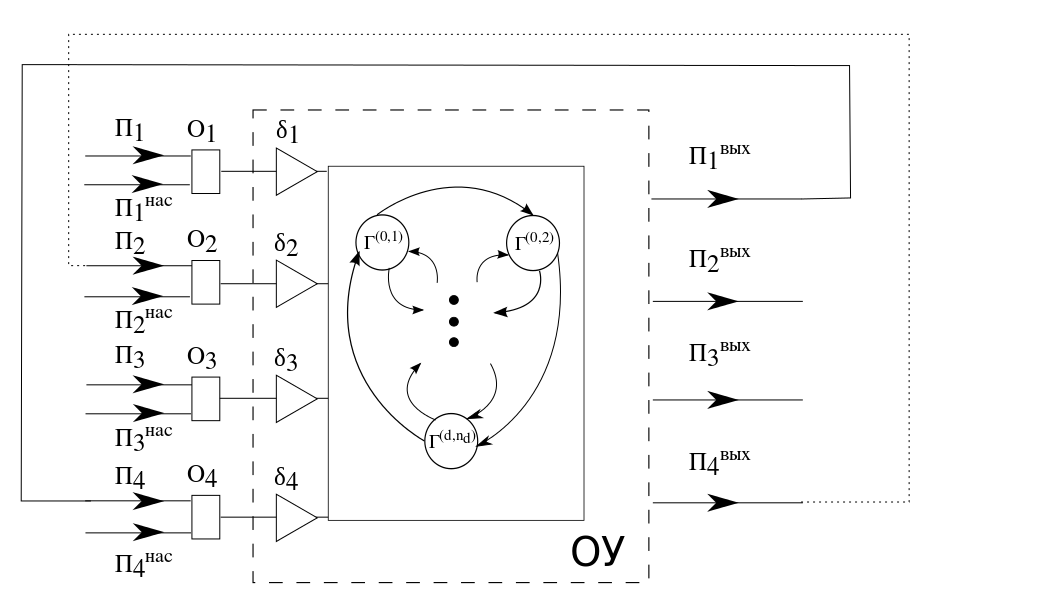
\includegraphics[scale=0.45]{SystemScheme.png} 
\caption{Структурная схема системы обслуживания}
\label{SystemScheme}
\end{figure}
Пусть в систему с одним обслуживающим устройством поступают потоки $\Pi_1$, $\Pi_2$, $\Pi_3$  и $\Pi_4$. Требования по потоку $\Pi_j$ становятся в соответствующую очередь $O_j$ с неограниченной вместимостью, $j\in \{1, 2, 3, 4\}$. Для $j \in \{1, 2, 3\}$ дисциплина очереди $O_j$, поддерживаемая устройством $\delta_j$, имеет тип FIFO (First In First Out). Таким образом, для обслуживания из соответствующей очереди выбирается то требование, которое пришло раньше. Дисциплина очереди $O_4$ будет описана ниже. Входные потоки $\Pi_1$ и $\Pi_3$ формируются внешней средой, которая, будем предполагать, имеет только одно состояние, то есть вероятностная структура потоков не меняется с течением времени. Требования потоков $\Pi_1$ и $\Pi_3$ формируют независимые между собой неординарные пуассоновские потоки, то есть  стационарные, без последействия и ординарные потоки групп требований. Интенсивности соответствующих простейших потоков для $\Pi_1$ и $\Pi_3$ будем обозначать $\lambda_1$ и $\lambda_3$, а распределение числа заявок в группе по потоку $\Pi_j$ будем описывать производящей функцией
\begin{equation}
f_j(z) = \sum_{\nu=1}^{\infty} p_{\nu}^{(j)} z ^{\nu}, \quad j\in \{1,3\},
\label{GeneratingFunc}
\end{equation}
которая предполагается аналитической при любом $z\in \mathbb{C}$ таком, что $|z|<(1+\varepsilon)$, $\varepsilon>0$. Величина $p_{\nu}^{(j)}$ определяет вероятность того, что по потоку $\Pi_j$ число требований в группе равно $\nu$. Обслуженные требования потока $\Pi_1$ поступают на повторное обслуживание, формируя на выходе поток $\Pi_4$. Обслуженные требования потока $\Pi_4$ в свою очередь поступают на повторное обслуживание, формируя при этом поток $\Pi_2$. Потоки $\Pi_2$ и $\Pi_3$ являются конфликтными, что означает запрет на одновременное обслуживание требований этих потоков и, следовательно, исследование системы не может быть сведено к задаче с меньшим числом потоков. 

В каждый момент времени обслуживающее устройство находится в одном из конечного множества состояний $\Gamma=\{\Gamma^{(k,r)} \colon k=\overline{0,d}; r=\overline{1,n_k}\}$ с заданными натуральными числами $d$, $n_0$, $n_1$, $\ldots$, $n_d$. В каждом состоянии $\Gamma^{(k,r)}$ обслуживающее устройство находится в течение времени $T^{(k,r)}$. Введем множества $\Gamma^{\mathrm{I}}$, $\Gamma^{\mathrm{II}}$, $\Gamma^{\mathrm{III}}$ и $\Gamma^{\mathrm{IV}}$ следующим образом. В состоянии $\gamma \in \Gamma^{\mathrm{\Rmnum{1}}}$ обслуживаются только требования из очередей $O_1$, $O_2$ и $O_4$.
В состоянии $\gamma \in \Gamma^{\mathrm{\Rmnum{2}}}$ обслуживаются только требования из очередей $O_2$ и $O_4$.
В состоянии $\gamma \in \Gamma^{\mathrm{\Rmnum{3}}}$ обслуживаются только требования из очередей $O_1$, $O_3$ и $O_4$.
В состоянии $\gamma \in \Gamma^{\mathrm{\Rmnum{4}}}$ обслуживаются только требования из очередей $O_3$ и $O_4$.
Тогда множество $\Gamma$ есть объединение $\Gamma = \Gamma^{\mathrm{I}} \cup \Gamma^{\mathrm{II}} \cup \Gamma^{\mathrm{III}} \cup \Gamma^{\mathrm{III}}$ непересекающихся подмножеств. Также в дальнейшем нам понадобятся множества ${}^1\Gamma=\Gamma^{\mathrm{\Rmnum{1}}} \cup \Gamma^{\mathrm{\Rmnum{3}}}$, 
${}^2\Gamma=\Gamma^{\mathrm{\Rmnum{1}}} \cup \Gamma^{\mathrm{\Rmnum{2}}}$,
${}^3\Gamma=\Gamma^{\mathrm{\Rmnum{3}}} \cup \Gamma^{\mathrm{\Rmnum{4}}}$. 

Смена состояний обслуживающего устройства осуществляется по следующему правилу. Множество состояний $C_k = \{\Gamma^{(k,r)} \colon r=\overline{1,n_k}\}$ будем называть $k$-м циклом, $k=\overline{1,d}$ (Рис. \ref{GraphScheme}). Состояние вида $\Gamma^{(0,r)}$ будем называть состоянием продления, $r=\overline{1,n_0}$. Положим $r \oplus_k 1 = r+1$ для $r=\overline{1,n_k-1}$ и $r \oplus_k 1 = 1$ при $r=n_k$, $k = \overline{0,d}$. В цикле $C_k$ выделим подмножества $C_k^{\mathrm{O}}$ выходных, $C_k^{\mathrm{I}}$ входных и $C_k^{\mathrm{N}} = C_k \setminus (C_k^{\mathrm{O}} \cup C_k^{\mathrm{I}})$ нейтральных состояний. Тогда после состояния $\Gamma^{(k,r)} \hm\in C_k\setminus C_k^{\mathrm{O}}$ обслуживающее устройство переходит в состояние $\Gamma^{(k,r \oplus_k 1)}$ того же цикла $C_k$. При $\Gamma^{(k,r)}$ принадлежащем множеству $C_k^{\mathrm{O}}$ прибор переходит в состояние $\Gamma^{(k,r \oplus_k 1)}$, если число требований в очереди $O_3$ в момент переключения больше заданного порога $L$. В противном случае, то есть если число требований в очереди $O_3$ меньше либо равно $L$, новое состояние прибора будет состоянием продления $\Gamma^{(0,r_1)}$, где $r_1=h_1(\Gamma^{(k,r)})$ и $h_1(\cdot)$~--- заданное отображение множества $\bigcup\limits_{k=1}^d C_k^{\mathrm{O}}$ во множество $\{1,2,\ldots, n_0\}$. После состояния $\Gamma^{(0,r)}$ выбирается состояние того же вида $\Gamma^{(0,r_2)}$, если число требований в очереди $O_3$ меньше или равно $L$, где $r_2=h_2(r)$ и $h_2(\cdot)$~--- заданное отображение множества $\{1,2, \ldots, n_0\}$ на себя; в противном случае включается входное состояние $\Gamma^{(k,r_3)} \in C_k^{\mathrm{I}}$, где $\Gamma^{(k,r_3)}=h_3(r)$ и $h_3(\cdot)$~--- заданное отображение множества $\{1,2, \ldots, n_0\}$ на множество  $\bigcup\limits_{k=1}^d C_k^{\mathrm{I}}$. Считается, что все состояния продления $\Gamma^{(0,r)}$ принадлежат множеству ${}^2 \Gamma$, а также верны соотношения $C_k^\mathrm{O}\subset {}^2 \Gamma$ и $C_k^\mathrm{I}\subset {}^3 \Gamma$. Также будем предполагать, что все циклы имеют ровно одно входное и одно выходное состояние. И последним предположением является то, что все вершины продления образуют один цикл, то есть можем положить $h_2(r)=r\oplus_0 1$.

\begin{figure}[h]\centering
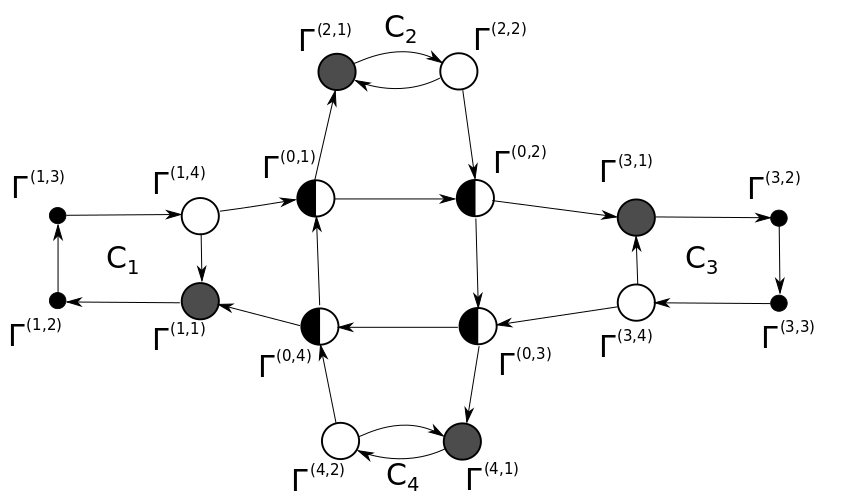
\includegraphics[scale=0.5]{GraphScheme3_grayscale.png} 
\caption{Класс графов переходов. Незакрашенные вершины являются выходными вершинами, Большие черные вершины --- входные, небольшие черные --- нейтральные, наполовину закрашенным вершинам соответствуют состояния продления}
\label{GraphScheme}
\end{figure}
%\subsection{Допустимые графы переходов состояний ОУ}

Таким образом, смена состояний обслуживающего устройства задается соотношением:
\begin{equation}
h(\Gamma^{(k,r)},y) = 
\begin{cases}
\Gamma^{(k,r \oplus_k 1)},& \quad \text{ если } (\Gamma^{(k,r)}\in C_k\setminus C_k^{\mathrm{O}}) \text{ или } (\Gamma^{(k,r)}\in C_k^{\mathrm{O}} \text{ \& } y>L);\\
%\Gamma^{(k,r \oplus_k 1)},& \quad \text{ если } \Gamma^{(k,r)}\in C_k^{\mathrm{O}} \text{ и } y>L;\\
\Gamma^{(0,h_1(\Gamma^{(k,r)}))},& \quad \text{ если } \Gamma^{(k,r)}\in C_k^{\mathrm{O}} \text{ и } y\leqslant L;\\
\Gamma^{(0,r \oplus_0 1)},& \quad \text{ если } k=0 \text{ и } y\leqslant L;\\
h_3(r),& \quad \text{ если } k=0 \text{ и } y > L.
\end{cases}
\label{hLaw}
\end{equation}

Рассмотрим введеные обозначения на примере рис.~\ref{GraphScheme}. Входными состояниями обслуживающего устройства являются $\Gamma^{(1,1)} \in C_1^{\mathrm{I}}$, $\Gamma^{(2,1)} \in C_2^{\mathrm{I}}$, $\Gamma^{(3,1)} \in C_3^{\mathrm{I}}$ и $\Gamma^{(4,1)} \in C_4^{\mathrm{I}}$, выходные состояния~--- $\Gamma^{(1,4)} \in C_1^{\mathrm{O}}$, $\Gamma^{(2,2)} \in C_2^{\mathrm{O}}$, $\Gamma^{(3,4)} \in C_3^{\mathrm{O}}$ и $\Gamma^{(4,2)} \in C_4^{\mathrm{O}}$, нейтральные состояния~--- $\Gamma^{(1,2)}, \Gamma^{(1,3)} \in C_1^{\mathrm{N}}$ и $\Gamma^{(3,2)}, \Gamma^{(3,3)} \in C_3^{\mathrm{N}}$. Состояния продления на графе представлены вершинами $\Gamma^{(0,1)}$, $\Gamma^{(0,2)}$, $\Gamma^{(0,3)}$ и $\Gamma^{(0,4)}$. Далее, отображение $h_1(\cdot)$ на графе задано таким образом, что оно переводит, например, выходное состояние $\Gamma^{(1,4)}$ в число $1$~--- номер состояния продления $\Gamma^{(0,1)}$, то есть $h_1(\Gamma^{(1,4)})=1$. Аналогично, например, $h_2(1)=2$ и $h_2(3)=4$. Примером отображения $h_3(\cdot)$ является $h_3(2)=\Gamma^{(3,1)}$.


Предполагается, что длительности обслуживания различных требований могут быть зависимыми и иметь различные законы распределения, поэтому вместо классического способа, состоящего в указании функции распределения длительности обслуживания произвольного требования, будут использованы потоки насыщения. Потоки насыщения $\Pi^{\mathrm{\text{нас}}}_j$, $j=\overline{1,4}$, определяются как виртуальные выходные потоки при условии максимального использования ресурсов обслуживающего устройства, а для $j=\overline{1,3}$ еще и при условии максимальной загрузки соответствующих очередей. 
Поток насыщения $\Pi^{\mathrm{\text{нас}}}_j$, $j=\overline{1,3}$, будет содержать неслучайное число $\ell(k,r,j)$ требований, обслуженных в течение времени $T^{(k,r)}$, если обслуживающее устройство находится в состоянии $\Gamma^{(k,r)}$. Пусть $\mathbb{Z}_+$~--- множество целых неотрицательных чисел. Тогда, при условии, что в очереди $O_4$ находится $x \in \mathbb{Z}_+$ требований, поток насыщения $\Pi^{\mathrm{\text{нас}}}_4$ определим как поток, содержащий все $x$ требований.
%\subsection{Пример: тандем из двух перекрестков} 
Наконец, при состоянии обслуживающего устройства $\Gamma^{(k,r)}$ каждое требование из очереди $O_4$ с вероятностью $p_{k,r}$ и независимо от других завершает обслуживание и отправляется в очередь $O_2$ потока~$\Pi_2$. С вероятностью $1-p_{k,r}$ требование очереди $O_4$ остается в ней до следующего такта. На следующем такте процесс повторяется.

В качестве наглядной физической интерпретации можно привести тандем из двух перекрестков (рис. \ref{crossroads}).
\begin{figure}[h]
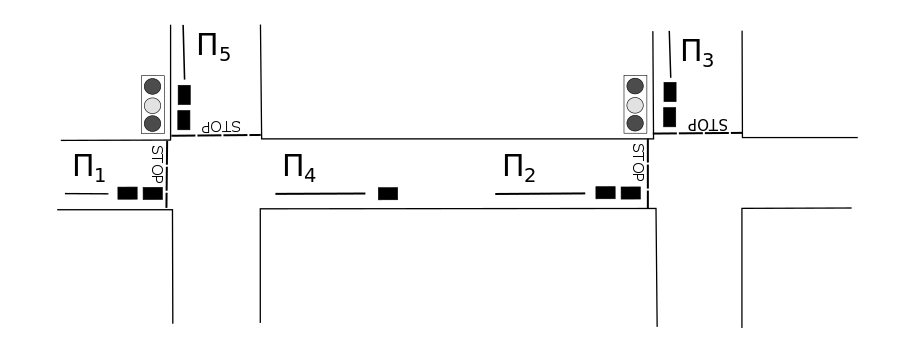
\includegraphics[scale=0.5]{Crossroads_grayscale.png} 
\caption{Пример: тандем перекрестков}
\label{crossroads}
\end{figure}
В качестве потоков требований, формируемых внешней средой, выступают потоки прибывающих на перекрестки машин: конфликтные потоки $\Pi_1$, $\Pi_5$ на первом перекрестке, а также поток $\Pi_3$ на втором. Каждая машина из потока $\Pi_1$, проезжая первый перекресток, становится в очередь $O_4$ потока $\Pi_4$ и затем с некой вероятностью ($p_{k,r}$ для состояния $\Gamma^{(k,r)}$ обслуживающего устройства) доезжает до следующего перекрестка, или же не успевает это сделать и остается в очереди $O_4$ до следующего такта обслуживания. В случае, если машина из очереди $O_4$ успевает доехать до второго перекрестка, она становится в очередь $O_2$ и ждет своей очереди для его прохождения.

Предполагается, что светофор на первом перекрестке имеет лишь два состояния $\{g_{1,1},g_{1,2}\}$: в состоянии $g_{1,1}$ машины потока $\Pi_1$ пропускаются фиксированное количество времени $\widetilde T^{(1,1)}$ (<<зеленый>> свет для $\Pi_1$); в состоянии $g_{1,2}$ --- простаивают в течение времени $\widetilde T^{(1,2)}$ (<<красный>> свет для $\Pi_1$). Светофор на втором перекрестке обслуживает по алгоритму с продлением: дополнительно к состоянию обслуживания потока $\Pi_3$ (состояние $g_{2,1}$), также имеется два состояния обслуживания потока $\Pi_2$ (состояния $\{g_{2,2},g_{2,3}\}$). Первое из них включается всегда после завершения обслуживания потока $\Pi_3$, а второе включается, если после очередного такта обслуживания потока $\Pi_2$ длина очереди $O_3$ не превосходит уровня $L$.
Длительности пребывания светофора на втором перекрестке в каждом из состояний суть $\widetilde T^{(2,1)}$, $\widetilde T^{(2,2)}$ и $\widetilde T^{(2,3)}$.


Рассматривая тандем из двух перекрестков как единую систему массового обслуживания и предполагая наблюдение за ней только в (дискретные) моменты переключения состояния хотя бы одного из светофоров, может быть показано, что количество различных состояний у полученной системы конечно. Действительно, положим, например, за состояние объединенной системы вектор $(g^{(1)},g^{(2)}, s, t)$, где $g^{(1)}\in \{g_{1,1},g_{1,2}\}$~--- состояние $1$--го перекрестка, $g^{(2)}\in \{g_{2,1},g_{2,2},g_{2,3}\}$~--- состояние $2$--го перекрестка, $s \in \{0, 1, 2\}$~--- номер последнего сменившего состояние перекрестка (принимает значение $0$ в случае, если сменили состояние оба перекрестка) и $t \in \{0, 1, 2, \ldots, T\}$~--- количество времени, оставшееся у продолжающего обслуживание с прошлого такта перекрестка (принимает значение $0$, если принимает значение $0$ величина $s$). Здесь $T$~--- максимальная длительность нахождения каждого из светофоров в одном состоянии. Тогда количество различных состояний не трудно посчитать и оно не будет превышать величины  $2\times 3 \times 3 \times T$.

В завершение построения примера отметим, что при прохождении перекрестков машины предполагаются движущимися только в прямом направлении, то есть перемешивания конфликтных потоков не допускается. Таким образом, поток $\Pi_5$ не представляет интереса для дальнейшего исследования системы и может быть отброшен и, следовательно, построенный пример целиком удовлетворяет структурной схеме на рис.~\ref{SystemScheme}.

Теперь продемонстрируем на конкретном числовом примере выделение циклов и состояний продления. Пусть изменение состояний перекрестков и время пребывания (в секундах для определнности) в каждом из состояний задается графами на рис. \ref{SystemStates}.
\begin{figure}[h]
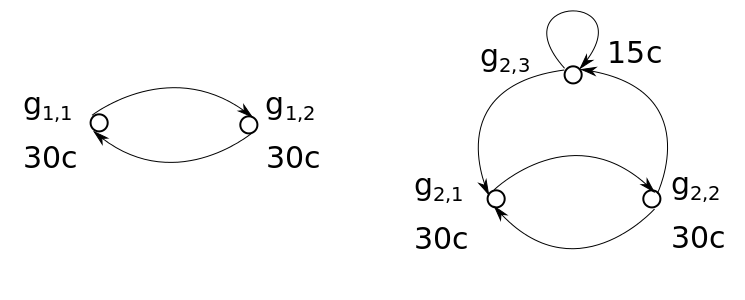
\includegraphics[scale=0.5]{SystemStates.png} 
\caption{Числовой пример тандема перекрестков. Левый граф соответствует первому перекрестку, правый~--- второму}
\label{SystemStates}
\end{figure}
За начальное состояние объединенной системы примем $\Gamma_0=(g_{1,1},g_{2,1},0,0)$, то есть первый перекресток находится в состоянии $g_{1,1}$, второй~--- в состоянии $g_{2,1}$, и оба только начали свою работу в своем состоянии (этот факт моделируется равенствами $s=0$ и $t=0$). Следующая смена состояний случится у обоих перекрестков одновременно и приведет к следующему состоянию $(g_{1,2},g_{2,2}, 0, 0)$. Далее смена состояний произойдет также у первого и второго перекрестков, однако второй перекресток может перейти как в состояние $g_{2,1}$, так и в состояние продления $g_{2,3}$. Таким образом следущим состоянием тандема будет либо опять $(g_{1,1},g_{2,1},0,0)$, либо $(g_{1,1},g_{2,3},0,0)$. Продолжая рассуждения аналогичным образом, получим следущий список всех возможных состояний системы:
\begin{align*}
(g_{1,1},g_{2,1},0,0)&=\Gamma^{(1,1)} ,& \quad (g_{1,2},g_{2,2},0,0)&=\Gamma^{(1,2)} ,& \quad (g_{1,1},g_{2,3},0,0)&=\Gamma^{(0,1)}, \\
(g_{1,1},g_{2,3},15,2)&=\Gamma^{(0,2)} ,& \quad (g_{1,2},g_{2,3},0,0)&=\Gamma^{(0,3)} ,& \quad (g_{1,2},g_{2,3},15,2)&=\Gamma^{(0,4)}, \\
(g_{1,2},g_{2,1},15,2)&=\Gamma^{(4,1)} ,& \quad (g_{1,1},g_{2,1},15,1)&=\Gamma^{(4,2)} ,& \quad (g_{1,1},g_{2,2},15,2)&=\Gamma^{(4,3)}, \\
(g_{1,2},g_{2,2},15,1)&=\Gamma^{(4,4)} ,& \quad (g_{1,2},g_{2,3},15,2)&=\Gamma^{(0,5)} ,& \quad (g_{1,2},g_{2,1},0,0)&=\Gamma^{(3,1)}, \\
(g_{1,1},g_{2,2},0,0)&=\Gamma^{(3,2)} ,& \quad (g_{1,1},g_{2,1},15,2)&=\Gamma^{(2,1)} ,& \quad (g_{1,2},g_{2,1},15,1)&=\Gamma^{(2,2)}, \\
(g_{1,2},g_{2,2},15,2)&=\Gamma^{(2,3)} ,& \quad (g_{1,1},g_{2,2},15,1)&=\Gamma^{(2,4)}. & &
\end{align*}
В соответсвии с приведенными выше обозначениями, множества $C_1$, $C_2$, $C_3$, $C_4$, а также множество состояний продления строятся однозначным образом. Множествами входных состояний будут $C_1^{\mathrm{I}}=\{\Gamma^{(1,1)}\}$, $C_2^{\mathrm{I}}=\{\Gamma^{(2,1)}\}$, $C_3^{\mathrm{I}}=\{\Gamma^{(3,1)}\}$ и $C_4^{\mathrm{I}}=\{\Gamma^{(4,1)}\}$. Множествами выходных состояний будут $C_1^{\mathrm{O}}=\{\Gamma^{(1,2)}\}$, $C_2^{\mathrm{O}}=\{\Gamma^{(2,4)}\}$, $C_3^{\mathrm{O}}=\{\Gamma^{(3,2)}\}$ и $C_4^{\mathrm{O}}=\{\Gamma^{(4,4)}\}$. Функции $h_1(\cdot)$, $h_2(\cdot)$ и $h_3(\cdot)$ задаются поточечно:
\begin{equation*}
h_1(\Gamma^{(1,2)})=1, \quad h_1(\Gamma^{(2,4)})=2, \quad h_1(\Gamma^{(3,2)})=3, \quad h_1(\Gamma^{(4,4)})=5,
\end{equation*}
\begin{equation*}
h_2(1)=2, \quad h_2(2)=3, \quad h_2(3)=4 \quad h_2(4)=1, \quad h_2(5)=1,
\end{equation*}
\begin{equation*}
h_3(1)=\Gamma^{(2,1)}, \quad h_3(2)=\Gamma^{(3,1)}, \quad h_3(3)=\Gamma^{(4,1)} \quad h_3(4)=\Gamma^{(1,1)}, \quad h_3(5)=\Gamma^{(1,1)}.
\end{equation*}
Этим завершается построение числового примера.

\subsection{Представление рассматриваемой системы обслуживания в виде кибернетической управляющей системы}
Описанная в предыдущем разделе на содержательном уровне система массового обслуживания должна рассматриваться как кибернетическая управляющая система обслуживания (см. \cite{Zorine:2011:2}). Схема управляющей системы приведена на рис. \ref{SystemScheme}. На схеме присутствуют следующие блоки: 1) внешняя среда с одним состоянием; 2) входные полюса первого типа~--- входные потоки $\Pi_1$, $\Pi_2$, $\Pi_3$, $\Pi_4$; 3) входные полюса второго типа~--- потоки насыщения $\Pi_1^{\mathrm{\text{нас}}}$, $\Pi_2^{\mathrm{\text{нас}}}$, $\Pi_3^{\mathrm{\text{нас}}}$, $\Pi_4^{\mathrm{\text{нас}}}$; 4) внешняя память~--- очереди $O_1$, $O_2$, $O_3$, $O_4$; 5) устройство по переработкe информации внешней памяти~--- устройства по поддержанию дисциплины очереди $\delta_1$, $\delta_2$, $\delta_3$, $\delta_4$; 6) внутренняя память~--- обслуживающее устройство (ОУ); 7) устройство по переработке информации во внутренней памяти~--- граф смены состояний; 8) выходные полюса $\Pi_1^{\mathrm{\text{вых}}}$, $\Pi_2^{\mathrm{\text{вых}}}$, $\Pi_3^{\mathrm{\text{вых}}}$, $\Pi_4^{\mathrm{\text{вых}}}$. Координатой блока является номер этого блока на схеме. 

Для задания информации блоков введем следующие величины и элементы, а также укажем множества их возможных значений. В качестве дискретной временной шкалы выберем последовательность $\tau_0=0$, $\tau_1$, $\tau_2$, $\ldots$ моментов смены состояния обслуживающего устройства. Обозначим $\Gamma_i$, $i\geqslant 1$, из множества $\Gamma$ состояние обслуживающего устройства в течение времени $\left(\tau_{i-1};\tau_i\right]$ и $\Gamma_0\in \Gamma$~--- в момент времени $\tau_0$, количество $\varkappa_{j,i} \in \mathbb{Z}_+ $, $i\geqslant 0$, требований в очереди $O_j$ в момент времени $\tau_i$, количество $\eta_{j,i} \in \mathbb{Z}_+$, $i\geqslant 0$, требований, поступивших в очередь $O_j$ по потоку $\Pi_j$ в течение времени $\left(\tau_{i};\tau_{i+1}\right]$, количество $\xi_{j,i} \in \mathbb{Z}_+$, $i\geqslant 0$, требований по потоку насыщения $\Pi^{\mathrm{\text{нас}}}_j$ в течение времени $\left(\tau_{i};\tau_{i+1}\right]$, количество $\overline{\xi}_{j,i}\in \mathbb{Z}_+$, $i\geqslant 0$, реально обслуженных требований по потоку $\Pi_j$ в течение времени $\left(\tau_{i};\tau_{i+1}\right]$; $j=\overline{1,4}$.

Закон изменения состояния обслуживающего устройства будем предполагать заданным соотношением 
\begin{equation}
\Gamma_{i+1}=h(\Gamma_i,\varkappa_{3,i}),
\label{gammaFunc}
\end{equation}
где отображение $h(\cdot,\cdot)$ определено в \eqref{hLaw}.
Для определения длительности $T_{i+1}$ состояния обслуживающего устройства в течение времени $\left(\tau_{i};\tau_{i+1}\right]$ удобно ввести функцию $h_T(\cdot,\cdot)$:
\begin{equation*}
T_{i+1}=h_T(\Gamma_i,\varkappa_{3,i})= T^{(k,r)},\quad  \text{ где $k$ и $r$ таковы, что } \Gamma^{(k,r)}=\Gamma_{i+1}=h(\Gamma_i,\varkappa_{3,i}).
%\label{timeLaw}
\end{equation*}
Функциональная зависимость
\begin{equation}
\overline{\xi}_{j,i}=\min\{\varkappa_{j,i}+\eta_{j,i},\xi_{j,i}\}, \quad j\in \{1,2,3\},
\label{saturationEq}
\end{equation}
между величиной $\overline{\xi}_{j,i}$ и величинами $\varkappa_{j,i}$, $\eta_{j,i}$, $\xi_{j,i}$ реализует стратегию механизма обслуживания требований. Далее, поскольку 
\begin{equation*}
\varkappa_{j,i+1}=\varkappa_{j,i}+\eta_{j,i}-\overline{\xi}_{j,i}, \quad  j\in \{1,2,3\},
\end{equation*}
то из выражения \eqref{saturationEq} следует соотношение
\begin{equation}
\varkappa_{j,i+1}=\max\{{0,\varkappa_{j,i}+\eta_{j,i}-\xi_{j,i}}\}, \quad j\in \{1,2,3\}.
\label{queuesFunc}
\end{equation}
Из формулировки поставленной задачи (см. также структурную схему на рис.~\ref{SystemScheme}) следуют соотношения для потока $\Pi_4$:
\begin{equation}
\eta_{4,i} = \min\{\xi_{1,i}, \varkappa_{1,i}+\eta_{1,i}\}, \quad \varkappa_{4,i+1}=\varkappa_{4,i}+\eta_{4,i}-\eta_{2,i}, \quad \xi_{4,i} = \varkappa_{4,i}.
\label{FourthFunc}
\end{equation}

Нелокальное описание входных потоков и потоков насыщения состоит в указании некоторых свойств условных распределений выделенных дискретных компонент $\eta_i=(\eta_{1,i},\eta_{2,i}, \eta_{3,i}, \eta_{4,i})$ и $\xi_i=(\xi_{1,i}, \xi_{2,i}, \xi_{3,i}, \xi_{4,i})$ маркированных точечных процессов \linebreak $\{(\tau_i, \nu_i, \eta_i); i\geqslant 0\}$ и $\{(\tau_i, \nu_i, \xi_i); i\geqslant 0\}$ при фиксированных значениях метки $\nu_i \hm= (\Gamma_i;\varkappa_i)$, где $\varkappa_i=(\varkappa_{1,i},\varkappa_{2,i},\varkappa_{3,i},\varkappa_{4,i})$. 
Введем функции $\varphi_1(\cdot,\cdot)$ и $\varphi_3(\cdot,\cdot)$ из разложений 
\begin{equation*}
\sum_{\nu=0}^{\infty} z^\nu\varphi_j(\nu,t) = \exp\{\lambda_j t (f_j(z)-1)\},
\end{equation*}
где $f_j(z)$ определены выражением \eqref{GeneratingFunc}, $j \in \{1,3\}$. Функция $\varphi_j(\nu,t)$ по своему смыслу есть вероятность поступления $\nu=0$, $1$, $\ldots$ требований по потоку $\Pi_j$ за время $t \geqslant 0$. Положим $\varphi_j(\nu,t)$ равной нулю при $\nu < 0$. Функцию $\psi(\cdot,\cdot,\cdot)$ зададим формулой
\begin{equation*}
\psi(k;y,u)=C_y^k u^k (1-u)^{y-k}.	
\end{equation*}
По своему смыслу $\psi(k;y,u)$ есть вероятность поступления $k$ требований по потоку $\Pi_2$ при условии, что очередь $O_4$ содержит $y$ требований и обслуживающее устройство находится в состоянии $\Gamma^{(k,r)}$, так что $u=p_{k,r}$. При нарушении условия $ 0\leqslant k \leqslant y$ положим $\psi(k;y,u)$ равной нулю.

Пусть $a=(a_1, a_2, a_3, a_4) \in \mathbb{Z}_+^4$ и $x=(x_1, x_2, x_3, x_4) \in \mathbb{Z}_+^4$. Тогда из постановки задачи на содержательном уровне следует, что при фиксированном значении метки $\nu_i=(\Gamma^{(k,r)}; x)$ вероятность $\varphi(a,k,r,x)$ одновременного выполнения равенств $\eta_{1,i}=a_1$, $\eta_{2,i}=a_2$, $\eta_{3,i}=a_3$, $\eta_{4,i}=a_4$ есть 
\begin{equation}
\varphi_1(a_1,h_T(\Gamma^{(k,r)},x_3)) \times \psi(a_2,x_4, p_{\tilde{k},\tilde{r}}) \times \varphi_3(a_3,h_T(\Gamma^{(k,r)},x_3))
\times \delta_{a_4,\min{\{\ell(\tilde{k},\tilde{r},1), x_1+a_1}\}},
\label{conditionProbOne}
\end{equation}
где $\tilde{k}$ и $\tilde{r}$ таковы, что $\Gamma^{(\tilde{k},\tilde{r})}=h(\Gamma^{(k,r)},x_3)$ и $\delta_{i,j}$ есть символ Кронекера:
%\begin{equation*}
$$
\delta_{i,j}=
\begin{cases} 
1,& \quad \text{ если $i=j$,}\\
0,& \quad \text{ если $i\neq j$.}
\end{cases}
$$%\end{equation*}
Пусть $b=(b_1, b_2, b_3, b_4) \in \mathbb{Z}_+^4$. Из содержательной постановки задачи также следует, что вероятность $\zeta(b, k, r, x)$ одновременного выполнения равенств $\xi_{1,i}=b_1$, $\xi_{2,i}=b_2$, $\xi_{3,i}=b_3$, $\xi_{4,i}=b_4$ при фиксированном значении $(\Gamma^{(k,r)}; x)$ метки $\nu_i$ есть
\begin{equation}
\delta_{b_1,\ell(\tilde{k},\tilde{r},1)} \times \delta_{b_2,\ell(\tilde{k},\tilde{r},2)} \times 
\delta_{b_3,\ell(\tilde{k},\tilde{r},3)} \times \delta_{b_4,x_4}.
\label{conditionProbTwo}
\end{equation}
Из формулы \eqref{conditionProbTwo} следует для $j\in \{1, 2, 3\}$, что вероятность события $\xi_{j,i}=0$ равна $1$ в случае $h(\Gamma^{(k,r)},x_3)\notin {}^j\Gamma$ и что вероятность события $\xi_{j,i}=\ell(\tilde{k},\tilde{r},j)$ равна $1$, если $\Gamma^{(\tilde{k},\tilde{r})}=h(\Gamma^{(k,r)},x_3)\in {}^j\Gamma$.


Содержательный смысл следующей теоремы состоит в том, что сформулированные выше функциональные связи и вероятностные свойства введенных объектов непротиворечивы и могут быть реализованы на некотором вероятностном пространстве.
%Построим теперь 	вероятностное пространство $(\Omega, {\cal F}, \Pr(\cdot))$, чтобы можно было рассматривать введеные величины как случайные величины на этом пространстве. А именно, докажем следующую теорему.

\begin{theorem}
Пусть $\gamma_0=\Gamma^{(k_0,r_0)}\in \Gamma$ и $x^0=(x_{1,0},x_{2,0}, x_{3,0},x_{4,0})\in \mathbb{Z}_+^4$ фиксированы.
Тогда существует вероятностное пространство $(\Omega, {\cal F}, \Pr(\cdot))$ и заданные на нем случайные величины $\eta_{j,i}=\eta_{j,i}(\omega)$, $\xi_{j,i}=\xi_{j,i}(\omega)$, 	 $\varkappa_{j,i}=\varkappa_{j,i}(\omega)$ и случайные элементы $\Gamma_i=\Gamma_i(\omega)$, $i\geqslant 0$, $j\in \overline{1,4}$, такие, что 1) имеют место равенства $\Gamma_0(\omega) = \gamma_0$ и $\varkappa_0(\omega)=x^0$; 2) выполняются соотношения \eqref{gammaFunc}, \eqref{queuesFunc}, \eqref{FourthFunc}; 3) для любых  $a\in \mathbb{Z}_+^4$, $b\in \mathbb{Z}_+^4$ и любых $x^t=(x_{1,t},x_{2,t},x_{3,t},x_{4,t}) \in \mathbb{Z}_+^4$, $\Gamma^{(k_t,r_t)} \in \Gamma$, $t = 1, 2, \ldots$, таких, что $\Pr\Bigl(\bigcap\limits_{t=0}^{i}\{\omega\colon \Gamma_t=\Gamma^{(k_t,r_t)}, \varkappa_t=x^t\}\Bigr)>0$, условное распределение векторов $\eta_i$ и $\xi_i$, $i \geqslant 0$,  имеет вид
\begin{equation}
\Pr \biggl(\{ \omega \colon \eta_i = a, \xi_i=b\} \bigg
|\,\bigcap_{t=0}^{i}\{\omega\colon \Gamma_t=\Gamma^{(k_t,r_t)}, \varkappa_t=x^t\}\biggr)=
\varphi(a,k_i,r_i,x^i)\times \zeta(b,k_i,r_i,x^i),
\label{ProbablititiesToProve}
\end{equation}
где функции $\varphi(\cdot, \cdot, \cdot, \cdot)$ и $\zeta(\cdot, \cdot, \cdot, \cdot)$ определяются формулами \eqref{conditionProbOne} и \eqref{conditionProbTwo}.

\label{myTheorem}
\end{theorem}
\begin{proof}
Для построения вероятностного пространства $(\Omega, {\cal F}, \Pr(\cdot))$ воспользуемся теоремой Ионеску Тулча (см. \cite{Shiryaev}, c. 348). 

Введем последовательность измеримых пространств $(\Omega_0, {\cal F}_0)$, $(\Omega_1, {\cal F}_1)$,$\ldots$, где $\Omega_i\hm=\mathbb{Z}_+^3$, $\omega_i=(\omega_{1,i},\omega_{2,i},\omega_{3,i}) \hm\in \Omega_i$, а $\sigma$-алгебра ${\cal F}_i=2^{\Omega_i}$  есть множество всех подмножеств множества $\Omega_i$. 
Пусть $\Gamma^{(\tilde{k},\tilde{r})}=h(\Gamma^{(k_0,r_0)},x_{3,0})$.
Зададим на измеримом пространстве $(\Omega_0, {\cal F}_0)$ вероятностную меру $P_0(\cdot)$ ее значениями на одноточечных множествах:
\begin{equation}
P_0(\{(a_1,a_2,a_3)\})=\varphi_1(a_1,h_T(\Gamma^{(k_0,r_0)})) \times \psi(a_2,x_{2,0}, p_{\tilde{k},\tilde{r}}) \times \varphi_3(a_3,h_T(\Gamma^{(k_0,r_0)})).
\label{probabilitiesOne}
\end{equation}

Для $j\in \{1,2,3\}$ определим величины
\begin{equation}
\tilde{\Gamma}_0(\omega_0)=\gamma_0, \quad \tilde{\varkappa}_{j,0}(\omega_0)=x_{j,0}, \quad \tilde{\xi}_{j,0}(\omega_0)=l(\tilde{k},\tilde{r},j), \quad \tilde{\eta}_{j,0}(\omega_0)=\omega_{j,0},
\label{startRekOne}
\end{equation}
и
\begin{equation}
 \tilde{\varkappa}_{4,0}(\omega_0)=x_{4,0}, \quad \tilde{\xi}_{4,0}(\omega_0)=x_{4,0}, \quad \tilde{\eta}_{4,0}(\omega_0)=\min\{\tilde{\xi}_{1,0}(\omega_0), \tilde{\varkappa}_{1,0}(\omega_0)+\tilde{\eta}_{1,0}(\omega_0)\}.
\label{startRekTwo}
\end{equation}

Теперь предположим, что заданы вероятностные меры $P_i(\omega_0\hm{}, \omega_1,\hm{} \ldots \hm{}, \omega_{i-1};\cdot)$ на измеримом пространстве $(\Omega_i, {\cal F}_i)$, $i=\overline{0,n}$,
и 
% определеныслучайные величины $\tilde{\Gamma}_i$, $\tilde{\varkappa}_{j,i}$, $\tilde{\xi}_{j,i}$, $\tilde{\eta}_{j,i}$, ч, и 
фиксирован набор $(\omega_0, \omega_1, \hm\ldots, \omega_{n})$. Положим для $j\in \{1, 2, 3\}$  и $i=\overline{0,n}$
\begin{equation}
\tilde{\Gamma}_{i+1}=\Gamma^{(k^*,r^*)}=h(\tilde{\Gamma}_{i},\tilde{\varkappa}_{3,i}), \quad \tilde{\varkappa}_{j,i+1}=\max\{ 0,\tilde{\varkappa}_{j,i}+\tilde{\eta}_{j,i} -\tilde{\xi}_{j,i}\},
\label{NextRekOne}
\end{equation}
\begin{equation}
\tilde{\varkappa}_{4,i+1}=\tilde{\varkappa}_{4,i}+\tilde{\eta}_{4,i}-\tilde{\eta}_{2,i}, \quad \tilde{\xi}_{j,i+1}=l(k^*,r^*,j),\quad \tilde{\eta}_{j,i+1}=\omega_{j,i+1}
\label{NextRekTwo}
\end{equation}
\begin{equation}
\tilde{\eta}_{4,i+1}=\min\{\tilde{\xi}_{1,i+1}, \tilde{\varkappa}_{1,i+1}+\tilde{\eta}_{1,i+1}\}, \quad \tilde{\xi}_{4,i+1}=\tilde{\varkappa}_{4,i+1}.
\label{NextRekThree}
\end{equation}
Заметим, что значения $\tilde{\Gamma}_{j,i}$, $\tilde\xi_{j,i}$, $\tilde\eta_{j,i}$, $\tilde\varkappa_{j,i}$, найденные по формулам \eqref{NextRekOne}--\eqref{NextRekThree} по наборам $(\omega_0, \omega_1,\ldots, \omega_n)$ и $(\omega_0, \omega_1,\ldots, \omega_i)$, $n\geqslant i$, совпадают.
Определим на измеримом пространстве $(\Omega_{n+1}, {\cal F}_{n+1})$ вероятностную меру  $P_{n+1}(\omega_0, \omega_1, \hm\ldots, \omega_n;\cdot)$
ее значениями на одноточечных множествах $\{(a_1,a_2,a_3)\}$, $(a_1,a_2,a_3)\hm\in {\mathbb Z}_+^3$:
\begin{multline}
P(\omega_0,\omega_1,\ldots,\omega_n;\{(a_1,a_2,a_3)\}) = \\
= \varphi_1(a_1,h_T(\tilde{\Gamma}_n,\tilde{\varkappa}_{3,n})) \times \psi(a_2,\tilde{\varkappa}_{4,n}, p_{k^*,r^*}) \times \varphi_3(a_3,h_T(\tilde{\Gamma}_n,\tilde{\varkappa}_{3,n})).
\label{probabilitiesTwo}
\end{multline}

%причем для любого множества $B\in {\cal F}_i$ функции $P(\omega_0,\omega_1,\hm\ldots,  \omega_{i-1};B)$ должны быть измеримыми функциями от $(\omega_0, \omega_1, \ldots, \omega_{i-1})$. 


Тогда (в соответствии с теоремой Ионеску Тулчи) для декартова произведения $\Omega=\prod\limits_{i=0}^{\infty}\Omega_i$ пространств элементарных исходов и произведения $\sigma$-алгебр ${\cal F}=\bigotimes\limits_{i=0}^{\infty} {\cal F}_i$ на $(\Omega,{\cal F})$ будет существовать единственная вероятностная мера $\Pr(\cdot)$ такая, что для любого $i \geqslant 0$ верно равенство
\begin{equation}
\Pr(\{\omega \colon \omega_0 \in A_0, \omega_1 \in A_1, \ldots, \omega_i\in A_i\})= P_i(A_0 \times A_1 \times \ldots \times A_i),
\label{ProbabilitiesGeneral}
\end{equation}
где 
\begin{equation}
 P_i(A_0 \times A_1 \times \ldots \times A_i) = \int_{A_0} P_0(d \omega_0) \int_{A_1} P_1(\omega_0;d \omega_1) \ldots \int_{A_i} P_i(\omega_0, \omega_1, \ldots, \omega_{i-1}; d \omega_i),
\label{ProbabilitiesGeneralOne}
\end{equation}
для любого $A_i$ из ${\cal F}_i$. Итак, вероятностное пространство $(\Omega,{\cal F},\Pr(\cdot))$ построено. 

Теперь введем на пространстве $(\Omega,{\cal F},\Pr(\cdot))$ следующие случайные величины и элементы, $i \geqslant 0$, $j =\overline{1,4}$:
\begin{equation*}
    \Gamma_i(\omega) = \tilde{\Gamma}_i, \quad \varkappa_{j,i}(\omega) = \tilde{\varkappa}_{j,i},\quad
    \xi_{j,i}(\omega) = \tilde{\xi}_{j,i}, \quad \eta_{j,i}(\omega) = \tilde{\eta}_{j,i}.
\end{equation*}
и докажем, что они  удовлетворяют условиям теоремы. Для сокращения записи зависимость от $\omega$ в обозначении случайных элементов и случайных величин далее будем опускать. Из формулы \eqref{NextRekOne} следует, что случайные элементы $\Gamma_i$ удовлетворяют соотношению \eqref{gammaFunc}, а случайные величины $\varkappa_{j,i}$ для $j\in \{1, 2, 3\}$ удовлетворяют соотношению \eqref{queuesFunc}. Из формулы \eqref{NextRekTwo} заключаем, что $\varkappa_{4,i}$ удовлетворяет соотношению $\eqref{FourthFunc}$. Далее, из условий \eqref{startRekTwo} и \eqref{NextRekThree} следует справедливость соотношений \eqref{FourthFunc} для величин $\eta_{4,i}$ и $\xi_{4,i}$. 

Перейдем к доказательству равенства \eqref{ProbablititiesToProve}. Для этого найдем явное выражение для условной вероятности $\Pr (\{ \omega \colon \eta_i = a, \xi_i=b\} | \bigcap_{t=0}^{i}\{\omega\colon \Gamma_t=\Gamma^{(k_t,r_t)}, \varkappa_t=x^t\})$. Пусть $\Gamma^{(\tilde{k}_i,\tilde{r}_i)}=h(\Gamma^{(k_i,r_i)},x^i)$. Запишем по определению условной вероятности, предполагая, что $\Pr\Bigl(\bigcap\limits_{t=0}^{i}\{\omega\colon \Gamma_t=\Gamma^{(k_t,r_t)}, \varkappa_t=x^t\}\Bigr)>0$:
\begin{multline}
\Pr \biggl(\left\{ \omega \colon \eta_i = a, \xi_i=b\right\}  \bigg| \bigcap_{t=0}^{i}\left\{\omega\colon \Gamma_t=\Gamma^{(k_t,r_t)}, \varkappa_t=x^t\right\}\biggr) = \\
=\Pr\biggl(\{ \omega \colon \eta_i = a, \xi_i=b \} \cap \bigcap_{t=0}^{i}\{\omega\colon \Gamma_t=\Gamma^{(k_t,r_t)}, \varkappa_t=x^t\}\biggr) \times \\
\times
\biggl(\Pr\biggl( \bigcap_{t=0}^{i}\{\omega\colon \Gamma_t=\Gamma^{(k_t,r_t)}, \varkappa_t=x^t\}\biggr)\biggr)^{-1}.
\label{Construction:1}
\end{multline}
Далее из соотношений \eqref{ProbabilitiesGeneral}, \eqref{ProbabilitiesGeneralOne} и того факта, что значения $\Gamma_i$ и $\varkappa_{i}$ зависят только от $\omega_0$, $\omega_1$ , $\ldots$, $\omega_{i-1}$, но не от $\omega_i$, (этот факт следует из формул \eqref{startRekOne}~--~\eqref{NextRekTwo}), получим выражение для второго сомножителя последнего выражения
\begin{multline}
\Pr\biggl( \bigcap_{t=0}^{i}\{\omega\colon \Gamma_t=\Gamma^{(k_t,r_t)}, \varkappa_t=x^t\}\biggr)=\\
=\sum_{\substack{\omega_0, \omega_1,\ldots, \omega_{i-1} \colon \\ \Gamma_t=\Gamma^{(k_t,r_t)},\, \varkappa_t=x^t,\\ t=\overline{0,i-1}}} P_0(\omega_0)\times P_1(\omega_0;\{\omega_1\})\times\ldots\times P_{i-1}(\omega_0,\omega_1,\ldots, \omega_{i-2};\{\omega_{i-1}\}).
\label{Construction:2}
\end{multline}
%Здесь мы положили $A_t(\omega_0,\omega_1,\ldots,\omega_{t-1})=\{\omega_t \colon \Gamma_t=\Gamma^{(k_t,r_t)}, \varkappa_t=x^t\}$, $t=\overline{0,i}$.

Преобразуем множество $\{\omega\colon \eta_i = a, \xi_i=b \} \cap \{\omega\colon\Gamma_i=\Gamma^{(k_i,r_i)}, \varkappa_i=x^i\}$, учитывая соотношения \eqref{startRekOne}~--~\eqref{NextRekThree}:
\begin{multline*}
\left\{\omega\colon \eta_i = a, \xi_i=b \right\} \cap \left\{\omega\colon\Gamma_i=\Gamma^{(k_i,r_i)}, \varkappa_i=x^i\right\} = \left\{\omega\colon\Gamma_i=\Gamma^{(k_i,r_i)}, \varkappa_i=x^i\right\} \cap\\
\cap \left\{\omega\colon \eta_{j,i} = a_j, j=\overline{1,3}\right\} \cap \left\{\omega\colon \xi_{j,i} = b_j, j=\overline{1,3}\right\} \cap \left\{ \omega\colon\xi_{4,i} = b_4 \right\} \cap  \left\{\omega\colon \eta_{4,i} = a_4 \right\} = \\
= \left\{\omega\colon\Gamma_i=\Gamma^{(k_i,r_i)}, \varkappa_i=x^i\right\} \cap \left\{\omega\colon \omega_{j,i} = a_j, j= \overline{1,3}\right\} \cap \left\{\omega\colon b_j=\ell(\tilde{k}_i,\tilde{r}_i,j), j=\overline{1,3}\right\} \cap \\ 
\cap \left\{ \omega\colon b_4 = x_{4,i} \right\} \cap  \left\{\omega\colon a_4=\min\left\{\ell(\tilde{k}_i,\tilde{r}_i,1), x_{1,i}+a_1\right\} \right\}. 
\end{multline*}
Тогда для второго множителя из правой части выражения \eqref{Construction:1} имеем:
\begin{multline}
\Pr\biggl(\{ \omega \colon \eta_i = a, \xi_i=b \} \cap \bigcap_{t=0}^{i}\{\omega\colon \Gamma_t=\Gamma^{(k_t,r_t)}, \varkappa_t=x^t\}\biggr)=\displaybreak[0]\\
= \Pr\biggl(\left\{\omega\colon \eta_i = a, \xi_i=b \right\} \cap \left\{\omega\colon\Gamma_i=\Gamma^{(k_i,r_i)}, \varkappa_i=x^i\right\} \cap \bigcap_{t=0}^{i-1}\{\omega\colon \Gamma_t=\Gamma^{(k_t,r_t)}, \varkappa_t=x^t\}\biggr)=\displaybreak[0]\\
= \delta_{b_4,x_{4,i}} \times \delta_{a_4,\min\left\{\ell(\tilde{k}_i,\tilde{r}_i,1), x_{1,i}+a_1\right\}} \times \prod_{j=1}^3\delta_{b_j,\ell(\tilde{k}_i,\tilde{r}_i,j)}   \times \displaybreak[0]\\
\times \Pr\biggl( \left\{ \omega\colon \omega_{j,i} = a_j, j=\overline{1,3}\right\} \cap \left\{\omega\colon\Gamma_i=\Gamma^{(k_i,r_i)}, \varkappa_i=x^i\right\}  \mathop{\cap}_{t=0}^{i-1}\{\omega\colon \Gamma_t=\Gamma^{(k_t,r_t)}, \varkappa_t=x^t\}\biggr).
\label{Construction:3}
\end{multline}
И по аналогии со вторым множителем в выражении \eqref{Construction:2} преобразуем последний сомножитель правой части равенства \eqref{Construction:3}:
\begin{multline*}
\Pr\biggl( \left\{ \omega \colon \omega_{j,i} = a_j,j=\overline{1,3}; \Gamma_i=\Gamma^{(k_i,r_i)}, \varkappa_i=x^i\right\} \cap \bigcap_{t=0}^{i-1}\{\omega\colon \Gamma_t=\Gamma^{(k_t,r_t)}, \varkappa_t=x^t\}\biggr) 
= \\ =\sum_{\substack{\omega_0, \omega_1,\ldots, \omega_{i-1} \colon \\ \Gamma_t=\Gamma^{(k_t,r_t)},\, \varkappa_t=x^t, \\ t=\overline{0,i-1}}} P_0(\omega_0)\times P_1(\omega_0;\{\omega_1\})\times\ldots \times P_{i-1}(\omega_0,\omega_1,\ldots, \omega_{i-2};\{\omega_{i-1}\})
\times \\[-2ex] \times P_i(\omega_0,\omega_1,\ldots, \omega_{i-1};\{(a_1, a_2, a_3)\})
\end{multline*}
и, учитывая выражение \eqref{probabilitiesTwo}, получим
\begin{multline}
\Pr\biggl( \left\{ \omega \colon \omega_{j,i} = a_j, j=\overline{1,3}; \Gamma_i=\Gamma^{(k_i,r_i)}, \varkappa_i=x^i\right\} \cap \bigcap_{t=0}^{i-1}\{\omega\colon \Gamma_t=\Gamma^{(k_t,r_t)}, \varkappa_t=x^t\}\biggr) 
=\\=\varphi_1(a_1,h_T(\Gamma_i,x_{3,i})) \times \psi(a_2,x_{4,i}, p_{\tilde{k}_i,\tilde{r}_i}) \times  \varphi_3(a_3,h_T(\Gamma_i,x_{3,i}))
\times \\ \times \sum_{\substack{\omega_0, \omega_1,\ldots, \omega_{i-1} \colon \\ \Gamma_t=\Gamma^{(k_t,r_t)},\, \varkappa_t=x^t,\\ t=\overline{0,i-1}}} P_0(\omega_0)\times P_1(\omega_0;\{\omega_1\})\times \ldots \times P_{i-1}(\omega_0,\omega_1,\ldots, \omega_{i-2};\{\omega_{i-1}\}).
\label{Construction:4}
\end{multline}

Подставляя выражение \eqref{Construction:4} в правую часть равенств \eqref{Construction:3}, а затем выражения  \eqref{Construction:3} и \eqref{Construction:2} в равенство \eqref{Construction:1}, получим:
\begin{multline*}
\Pr \biggl(\left\{ \omega \colon \eta_i = a, \xi_i=b\right\}  \biggl| \bigcap_{t=0}^{i}\left\{\omega\colon \Gamma_t=\Gamma^{(k_t,r_t)}, \varkappa_t=x^t\right\}\biggr.\biggr)  = \\
= \delta_{b_4,x_{4,i}} \times \delta_{a_4,\min\left\{\ell(\tilde{k}_i,\tilde{r}_i,1), x_{1,i}+a_1\right\}} \times \prod_{j=1}^3\delta_{b_j,\ell(\tilde{k}_i,\tilde{r}_i,j)} \times
\varphi_1(a_1,h_T(\Gamma_i,x_{3,i})) \times \\ \times \psi(a_2,x_{4,i}, p_{\tilde{k}_i,\tilde{r}_i}) 
\times  \varphi_3(a_3,h_T(\Gamma_i,x_{3,i})) \times\displaybreak[0] \\ 
\times \sum_{\substack{\omega_0, \omega_1,\ldots \omega_{i-1} \colon \\ \Gamma_t=\Gamma^{(k_t,r_t)}, \varkappa_t=x^t, \forall 0\leqslant t \leqslant i-1}} P_0(\omega_0)\times P_1(\omega_0;\{\omega_1\})\times\ldots\times P_{i-1}(\omega_0,\omega_1,\ldots, \omega_{i-2};\{\omega_{i-1}\}) \times \\
\times \raisebox{-1ex}{$\mathsurround=0pt \Biggl($} \sum_{\substack{\omega_0, \omega_1,\ldots \omega_{i-1} \colon \\ \Gamma_t=\Gamma^{(k_t,r_t)}, \varkappa_t=x^t, \forall 0\leqslant t \leqslant i-1}} P_0(\omega_0)\times P_1(\omega_0;\{\omega_1\})\times\ldots\times P_{i-1}(\omega_0,\omega_1,\ldots, \omega_{i-2};\{\omega_{i-1}\})\raisebox{-1ex}{$\mathsurround=0pt \Biggr)$}^{-1}
\end{multline*}
и после сокращения одинаковых сумм получаем в точности требуемое равенство \eqref{ProbablititiesToProve}.
\end{proof}

\begin{corollary}\label{eta:xi:forget}
В условиях предыдущей теоремы верно равенство
\begin{multline}
\Pr \biggl(\{ \omega \colon \eta_i = a, \xi_i=b\} \left|\bigcap_{t=0}^{i}\{\omega\colon \Gamma_t=\Gamma^{(k_t,r_t)}, \varkappa_t=x^t\}\right.\biggr)=\\
=\Pr \biggl(\{ \omega \colon \eta_i = a, \xi_i=b\} \left|\{\omega\colon \Gamma_i=\Gamma^{(k_i,r_i)}, \varkappa_i=x^i\}\right.\biggr).
\label{eta:xi:forgetProperty}
\end{multline}
\end{corollary}
\begin{proof}
Действительно, из формулы \eqref{ProbablititiesToProve} cледует, что вероятность, стоящая в левой части равенства \eqref{eta:xi:forgetProperty}, равна величине $\varphi(a,k_i,r_i,x^i)\times \zeta(b,k_i,r_i,x^i)$, зависящей только от значения $(\Gamma^{(k_i,r_i)},x^i)$ пары $(\Gamma_i,\varkappa_i)$ и не зависящей от значений остальных пар $(\Gamma_t,\varkappa_t)_{0\leqslant t \leqslant i-1}$. 

Использовав формулу полной вероятности, получим для правой части равенства \eqref{eta:xi:forgetProperty}:
\begin{multline*}
 \Pr \biggl(\{ \omega \colon \eta_i = a, \xi_i=b\} \left|\{\omega\colon \Gamma_i=\Gamma^{(k_i,r_i)}, \varkappa_i=x^i\}\right.\biggr) = \\ = \sum_{t=0}^{i-1}\sum_{\Gamma_t\in \Gamma, \varkappa_t \in Z^4_+}\Pr \biggl(\{ \omega \colon \eta_i = a, \xi_i=b\} \biggl|\bigcap_{t=0}^{i}\{\omega\colon \Gamma_t=\Gamma^{(k_t,r_t)}, \varkappa_t=x^t\}\biggr) \times \\ \times \Pr \biggl(\{ \omega \colon  \Gamma_t=\Gamma^{(k_t,r_t)}, \varkappa_t=x^t\}\biggr) = 
 \varphi(a,k_i,r_i,x^i)\times \zeta(b,k_i,r_i,x^i) \times \\ \times \sum_{t=0}^{i-1}\sum_{\Gamma_t\in \Gamma, \varkappa_t \in Z^4_+}\Pr \biggl(\{ \omega \colon  \Gamma_t=\Gamma^{(k_t,r_t)}, \varkappa_t=x^t\}\biggr) =\varphi(a,k_i,r_i,x^i)\times \zeta(b,k_i,r_i,x^i).
\end{multline*}
Поскольку левая часть выражения \eqref{eta:xi:forgetProperty} равна правой, то следствие доказано. 
\end{proof}

Введем для $y_0$, $y$, $\tilde{y} \in \mathbb{Z}_+$ и $t \in \mathbb{R}$, $t\geqslant 0$ функции
\begin{equation}
\begin{aligned}
\widetilde{\psi}(k,r,y_0,y,\tilde{y}) &= 
(1 - \delta_{\tilde{y},0}) \psi(\tilde{y}+\ell(k,r,2)-y,y_0, p_{k,r}) + \delta_{\tilde{y},0}\sum_{a=0}^{\ell(k,r,2)-y} \psi(a,y_0, p_{k,r}),\\
\widetilde{\varphi}_1(k,r,t,y,\tilde{y}) &= (1-\delta_{\tilde{y},0}) \varphi_1(\tilde{y} + \ell(k,r,1)-y,t)  +\delta_{\tilde{y},0}\sum_{a=0}^{\ell(k,r,1)-y} \varphi_1(a,t),\\
\widetilde{\varphi}_3(k,r,t,y,\tilde{y}) &= (1-\delta_{\tilde{y},0}) \varphi_3(\tilde{y} + \ell(k,r,3)-y,t)  +\delta_{\tilde{y},0}\sum_{a=0}^{\ell(k,r,3)-y} \varphi_3(a,t).
\end{aligned}
\label{tildephi}
\end{equation}
причем $k$ и $r$ таковы, что $\Gamma^{(k,r)}\in \Gamma$.
	
\begin{corollary}
Пусть $\Gamma^{(k_{i+1},r_{i+1})}=h(\Gamma^{(k_i,r_i)},x_{3,i})$, $i=0$, $1$, $\ldots$. Тогда в условиях теоремы~\ref{myTheorem} верно равенство
\begin{equation}
\Pr (\{ \omega \colon \varkappa_{2,i+1} = x_{2,i+1}\} \mid\mathop{\cap}\limits_{t=0}^{i}\{\omega\colon \Gamma_t=\Gamma^{(k_t,r_t)}, \varkappa_t=x^t\})=\widetilde{\psi}(k_{i+1},r_{i+1},x_{4,i},x_{2,i},x_{2,i+1}),
\label{kappa:2:conditional}
\end{equation}
\end{corollary}
\begin{proof}
Запишем по формуле полной вероятности:
\begin{multline*}
\Pr (\{ \omega \colon \varkappa_{2,i+1} = x_{2,i+1}\} |\cap_{t=0}^{i}\{\omega\colon \Gamma_t=\Gamma^{(k_t,r_t)}, \varkappa_t=x^t\}) = \\
= \sum_{a,b\in \mathbb{Z}_+^4} \Pr (\{ \omega \colon \eta_i=a, \xi_i=b\} |\cap_{t=0}^{i}\{\omega\colon \Gamma_t=\Gamma^{(k_t,r_t)}, \varkappa_t=x^t\}) \times \\
\times \Pr (\{ \omega \colon \varkappa_{2,i+1} = x_{2,i+1}\} |\{\omega\colon \eta_i=a, \xi_i=b\}\cap \cap_{t=0}^{i}\{\omega\colon \Gamma_t=\Gamma^{(k_t,r_t)}, \varkappa_t=x^t\}).
\end{multline*}
Поскольку для величин $\varkappa_{2,i+1}$, $\eta_i$ и $\xi_i$ история до момента времени $\tau_i$ значения не имеет (см. формулы \eqref{eta:xi:forgetProperty} и \eqref{queuesFunc}), то
\begin{multline*}
\Pr (\{ \omega \colon \varkappa_{2,i+1} = x_{2,i+1}\} |\mathop{\cap}\limits_{t=0}^{i}\{\omega\colon \Gamma_t=\Gamma^{(k_t,r_t)}, \varkappa_t=x^t\}) = \\
=\sum_{a,b\in \mathbb{Z}_+^4} \Pr (\{ \omega \colon \eta_i=a, \xi_i=b\} |\{\omega\colon \Gamma_i=\Gamma^{(k_i,r_i)}, \varkappa_i=x^i\}) \times \\
\times \Pr (\{ \omega \colon \varkappa_{2,i+1} = x_{2,i+1}\} |\{\omega\colon \eta_i=a, \xi_i=b, \Gamma_i=\Gamma^{(k_i,r_i)}, \varkappa_i=x^i\}) 
\end{multline*}
и, учитывая формулу \eqref{ProbablititiesToProve}, продолжим
\begin{multline*}
\Pr (\{ \omega \colon \varkappa_{2,i+1} = x_{2,i+1}\} |\mathop{\cap}\limits_{t=0}^{i}\{\omega\colon \Gamma_t=\Gamma^{(k_t,r_t)}, \varkappa_t=x^t\}) =\\
=\sum_{a,b\in \mathbb{Z}_+^4} \varphi(a,k_i,r_i,x^i)\zeta(b,k_i,r_i,x^i) \times\\
\times \Pr (\{ \omega \colon \varkappa_{2,i+1} = x_{2,i+1}\} |\{\omega\colon \eta_i=a, \xi_i=b, \Gamma_i=\Gamma^{(k_i,r_i)}, \varkappa_i=x^i\}).
\end{multline*}

Функциональная зависимость \eqref{queuesFunc} позволяет упростить последнюю вероятность:
\begin{multline*}
\Pr (\{ \omega \colon \varkappa_{2,i+1} = x_{2,i+1}\} |\mathop{\cap}\limits_{t=0}^{i}\{\omega\colon \Gamma_t=\Gamma^{(k_t,r_t)}, \varkappa_t=x^t\}) =\\
=\sum_{a,b\in \mathbb{Z}_+^4} \varphi(a,k_i,r_i,x^i)\zeta(b,k_i,r_i,x^i)  \delta_{x_{2,i+1},\max\{0,x_{2,i}+a_2-b_2\}}.
\end{multline*}

Учтем явное выражение функций $\varphi(\cdot, \cdot, \cdot, \cdot)$ и $\zeta(\cdot, \cdot, \cdot, \cdot)$ из определений \eqref{conditionProbOne} и \eqref{conditionProbTwo}:
\begin{multline*}
\Pr (\{ \omega \colon \varkappa_{2,i+1} = x_{2,i+1}\} |\mathop{\cap}\limits_{t=0}^{i}\{\omega\colon \Gamma_t=\Gamma^{(k_t,r_t)}, \varkappa_t=x^t\}) =\\
=  \sum_{a,b\in \mathbb{Z}_+^4} \varphi_1(a_1,h_T(\Gamma^{(k_i,r_i)},x_{3,i})) \times \psi(a_2,x_{4,i}, p_{k_{i+1},r_{i+1}})  \times \varphi_3(a_3,h_T(\Gamma^{(k_i,r_i)},x_{3,i})) \times \\ \times \delta_{a_4,\min{\{\ell(k_{i+1},r_{i+1},1), x_{1,i}+a_1}\}} \times \delta_{b_1,\ell(k_{i+1},r_{i+1},1)} \delta_{b_2,\ell(k_{i+1},r_{i+1},2)} 
\delta_{b_4,x_{4,i}}. \delta_{x_{2,i+1},\max\{0,x_{2,i}+a_2-b_2\}} 
\end{multline*}
и перегруппируем множители:
\begin{multline*}
\Pr (\{ \omega \colon \varkappa_{2,i+1} = x_{2,i+1}\} |\mathop{\cap}\limits_{t=0}^{i}\{\omega\colon \Gamma_t=\Gamma^{(k_t,r_t)}, \varkappa_t=x^t\}) =\\
= \sum_{a_2,b_2\in \mathbb{Z}_+}\psi(a_2,x_{4,i}, p_{k_{i+1},r_{i+1}})  \delta_{b_2,\ell(k_{i+1},r_{i+1},2)}   \delta_{x_{2,i+1},\max\{0,x_{2,i}+a_2-b_2\}} \times \\ 
\times \sum_{a_3\in \mathbb{Z}_+} \varphi_3(a_3,h_T(\Gamma^{(k_i,r_i)},x_{3,i})) \times \sum_{a_1\in \mathbb{Z}_+} \varphi_1(a_1,h_T(\Gamma^{(k_i,r_i)},x_{3,i})) \times \\ 
\times \sum_{a_4\in \mathbb{Z}_+} \delta_{a_4,\min{\{\ell(k_{i+1},r_{i+1},1), x_{1,i}+a_1}\}} \sum_{b_1\in \mathbb{Z}_+} \delta_{b_1,\ell(k_{i+1},r_{i+1},1)} \sum_{b_3\in \mathbb{Z}_+} \delta_{b_3,\ell(k_{i+1},r_{i+1},3)} 
\times \sum_{b_4\in \mathbb{Z}_+}  \delta_{b_4,x_{4,i}}.
\end{multline*}
Поскольку все суммы кроме первой равны единице, то искомая вероятность упрощается следующим образом:
\begin{multline*}
\Pr (\{ \omega \colon \varkappa_{2,i+1} = x_{2,i+1}\} |\mathop{\cap}\limits_{t=0}^{i}\{\omega\colon \Gamma_t=\Gamma^{(k_t,r_t)}, \varkappa_t=x^t\}) =\\
=\sum_{a_2,b_2\in \mathbb{Z}_+}\psi(a_2,x_{4,i}, p_{k_{i+1},r_{i+1}})  \delta_{b_2,\ell(k_{i+1},r_{i+1},2)}   \delta_{x_{2,i+1},\max\{0,x_{2,i}+a_2-b_2\}}= \\
=\sum_{a_2\in \mathbb{Z}_+}\psi(a_2,x_{4,i}, p_{k_{i+1},r_{i+1}})   \delta_{x_{2,i+1},\max\{0,x_{2,i}+a_2-\ell(k_{i+1},r_{i+1},2)\}}.
\end{multline*}
В случае, когда $x_{2,i+1}$ больше $0$, величина $\delta_{x_{2,i+1},\max\{0,x_{2,i}+a_2-\ell(k_{i+1},r_{i+1},2)\}}$ отлична от нуля только при $x_{2,i+1}=x_{2,i}+a_2-\ell(k_{i+1},r_{i+1},2)$, то есть при $a_2=x_{2,i+1}-x_{2,i}\hm+\ell(k_{i+1},r_{i+1},2)$. В случае, когда $x_{2,i+1}$ равно $0$, величина $\delta_{x_{2,i+1},\max\{0,x_{2,i}+a_2-\ell(k_{i+1},r_{i+1},2)\}}$ отлична от нуля только при $ a_2\leqslant \ell(k_{i+1},r_{i+1},2)-x_{2,i}$. Таким образом,
\begin{multline*}
\Pr (\{ \omega \colon \varkappa_{2,i+1} = x_{2,i+1}\} |\mathop{\cap}\limits_{t=0}^{i}\{\omega\colon \Gamma_t=\Gamma^{(k_t,r_t)}, \varkappa_t=x^t\}) = \\
= \sum_{a_2\in \mathbb{Z}_+}\psi(a_2,x_{4,i}, p_{k_{i+1},r_{i+1}})   \delta_{x_{2,i+1},\max\{0,x_{2,i}+a_2-\ell(k_{i+1},r_{i+1},2)\}} = \displaybreak[0]\\
=(1 - \delta_{x_{2,i+1},0})\psi(x_{2,i+1}-x_{2,i}+\ell(k_{i+1},r_{i+1},2),x_{4,i}, p_{k_{i+1},r_{i+1}})  +\displaybreak[0] \\
+ \delta_{x_{2,i+1},0}\sum_{a=0}^{\ell(k_{i+1},r_{i+1},2)-x_{2,i}} \psi(a,x_{4,i}, p_{k_{i+1},r_{i+1}})= \widetilde{\psi}(k_{i+1},r_{i+1},x_{4,i},x_{2,i},x_{2,i+1})
\end{multline*}
и равенство \eqref{kappa:2:conditional} доказано.
\end{proof}

\begin{corollary}
Пусть $\Gamma^{(k_{i+1},r_{i+1})}=h(\Gamma^{(k_i,r_i)},x_{3,i})$, $i=0$, $1$, $\ldots$. Тогда в условиях теоремы~\ref{myTheorem} верно равенство
\begin{multline}
\Pr (\{ \omega \colon \varkappa_{3,i+1} = x_{3,i+1}\} |\mathop{\cap}\limits_{t=0}^{i}\{\omega\colon \Gamma_t=\Gamma^{(k_t,r_t)}, \varkappa_t=x^t\})=\displaybreak[0]\\
=\widetilde{\varphi}_3(k_{i+1},r_{i+1},h_T(\Gamma^{(k_i,r_i)},x_{3,i}),x_{3,i},x_{3,i+1}).
\label{kappa:3:conditional}
\end{multline}
\end{corollary}
\begin{proof}
Запишем по формуле полной вероятности с учетом формул \eqref{ProbablititiesToProve} и \eqref{eta:xi:forgetProperty}:
\begin{multline*}
\Pr (\{ \omega \colon \varkappa_{3,i+1} = x_{3,i+1}\} |\mathop{\cap}\limits_{t=0}^{i}\{\omega\colon \Gamma_t=\Gamma^{(k_t,r_t)}, \varkappa_t=x^t\})=\sum_{a,b\in \mathbb{Z}_+^4} \varphi(a,k_i,r_i,x^i)\times\\
 \times \zeta(b,k_i,r_i,x^i) \times \Pr (\{ \omega \colon \varkappa_{3,i+1} = x_{3,i+1}\} |\{\omega\colon \eta_i=a, \xi_i=b, \Gamma_i=\Gamma^{(k_i,r_i)}, \varkappa_i=x^i\}).
\end{multline*}

Из условия \eqref{queuesFunc} следует
\begin{multline*}
\Pr (\{ \omega \colon \varkappa_{3,i+1} = x_{3,i+1}\} |\mathop{\cap}\limits_{t=0}^{i}\{\omega\colon \Gamma_t=\Gamma^{(k_t,r_t)}, \varkappa_t=x^t\})=\\
= \sum_{a,b\in \mathbb{Z}_+^4} \varphi(a,k_i,r_i,x^i)\zeta(b,k_i,r_i,x^i)  \delta_{x_{3,i+1},\max\{0,x_{3,i}+a_3-b_3\}} 
\end{multline*}
и, раскрывая по определению $\varphi(\cdot, \cdot, \cdot, \cdot)$ и $\zeta(\cdot, \cdot, \cdot, \cdot)$, получим
\begin{multline*}
\Pr (\{ \omega \colon \varkappa_{3,i+1} = x_{3,i+1}\} |\mathop{\cap}\limits_{t=0}^{i}\{\omega\colon \Gamma_t=\Gamma^{(k_t,r_t)}, \varkappa_t=x^t\})=\\= \sum_{a_3,b_3\in \mathbb{Z}_+} \varphi_3(a_3,h_T(\Gamma^{(k_i,r_i)},x_{3,i})) \delta_{b_3,\ell(k_{i+1},r_{i+1},3)} \delta_{x_{3,i+1},\max\{0,x_{3,i}+a_3-b_3\}} \times \\
\times
\sum_{a_2\in \mathbb{Z}_+} \psi(a_2,x_{4,i}, p_{k_{i+1},r_{i+1}}) 
\times \sum_{a_1\in \mathbb{Z}_+}  \varphi_1(a_1,h_T(\Gamma^{(k_i,r_i)},x_{3,i})) \sum_{a_4\in \mathbb{Z}_+} \delta_{a_4,\min{\{\ell(k_{i+1},r_{i+1},1), x_{1,i}+a_1}\}} \times \\ \times  \sum_{b_1\in \mathbb{Z}_+}  \delta_{b_1,\ell(k_{i+1},r_{i+1},1)} 
\sum_{b_2\in \mathbb{Z}_+}  \delta_{b_2,\ell(k_{i+1},r_{i+1},2)} \times \\
\times  \sum_{b_4\in \mathbb{Z}_+}\delta_{b_4,x_{4,i}} =  \sum_{a_3\in \mathbb{Z}_+} \varphi_3(a_3,h_T(\Gamma^{(k_i,r_i)},x_3))  \delta_{x_{3,i+1},\max\{0,x_{3,i}+a_3-\ell(k_{i+1},r_{i+1},3)\}}.
\end{multline*}
И результат леммы получаем после следующих преобразований:
\begin{multline*}
\Pr (\{ \omega \colon \varkappa_{3,i+1} = x_{3,i+1}\} |\mathop{\cap}\limits_{t=0}^{i}\{\omega\colon \Gamma_t=\Gamma^{(k_t,r_t)}, \varkappa_t=x^t\})=\\
=\sum_{a_3\in \mathbb{Z}_+} \varphi_3(a_3,h_T(\Gamma^{(k_i,r_i)},x_{3,i}))  \delta_{x_{3,i+1},\max\{0,x_{3,i}+a_3-\ell(k_{i+1},r_{i+1},3)\}}  = \\
=(1 - \delta_{x_{3,i+1},0})\varphi_3(x_{3,i+1}-x_{3,i} + \ell(k_{i+1},r_{i+1},3),h_T(\Gamma^{(k_i,r_i)},x_{3,i})) 
+\delta_{x_{3,i+1},0}\times\\\times\sum_{a=0}^{\ell(k_{i+1},r_{i+1},3)-x_{3,i}} \varphi_3(a,h_T(\Gamma^{(k_i,r_i)},x_{3,i})) 
=\widetilde{\varphi}_3(k_{i+1},r_{i+1},h_T(\Gamma^{(k_i,r_i)},x_{3,i}),x_{3,i},x_{3,i+1}).\qedhere
\end{multline*}
\end{proof}

\begin{corollary}
Пусть $\Gamma^{(k_{i+1},r_{i+1})}=h(\Gamma^{(k_i,r_i)},x_{3,i})$, $i=0$, $1$, $\ldots$. Тогда в условиях теоремы~\ref{myTheorem} для $i \geqslant 0$ верны равенства
\begin{multline}
\Pr (\{ \omega \colon \varkappa_{1,i+1} = x_{1,i+1}, \varkappa_{3,i+1} = x_{3,i+1}\} |\mathop{\cap}\limits_{t=0}^{i}\{\omega\colon \Gamma_t=\Gamma^{(k_t,r_t)}, \varkappa_t=x^t\})=\\
=\widetilde{\varphi}_3(k_{i+1},r_{i+1},h_T(\Gamma^{(k_i,r_i)},x_{3,i}),x_{3,i},x_{3,i+1}) \times \widetilde{\varphi}_1(k_{i+1},r_{i+1},h_T(\Gamma^{(k_i,r_i)},x_{3,i}),x_{1,i},x_{1,i+1}).
\label{kappa:1:kappa:3:conditional}
\end{multline}
\end{corollary}
\begin{proof}
Доказательство проводится аналогично доказательству предыдущего следствия. А именно, записывая по формуле полной вероятности с учетом формул \eqref{ProbablititiesToProve} и \eqref{eta:xi:forgetProperty}, имеем:
\begin{multline*}
\Pr (\{ \omega \colon \varkappa_{1,i+1} = x_{1,i+1}, \varkappa_{3,i+1} = x_{3,i+1} |\mathop{\cap}\limits_{t=0}^{i}\{\omega\colon \Gamma_t=\Gamma^{(k_t,r_t)}, \varkappa_t=x^t\}) =\\
=\sum_{a,b\in \mathbb{Z}_+^4} \varphi(a,k_i,r_i,x^i)\zeta(b,k_i,r_i,x^i) \times\\
\times \Pr (\{ \omega \colon \varkappa_{1,i+1} = x_{1,i+1}, \varkappa_{3,i+1} = x_{3,i+1}\} |\{\omega\colon \eta_i=a, \xi_i=b, \Gamma_i=\Gamma^{(k_i,r_i)}, \varkappa_i=x^i\}).
\end{multline*}


Из условий \eqref{queuesFunc} опять следует
\begin{multline*}
\Pr (\{ \omega \colon \varkappa_{1,i+1} = x_{1,i+1}, \varkappa_{3,i+1} = x_{3,i+1}\} |\mathop{\cap}\limits_{t=0}^{i}\{\omega\colon \Gamma_t=\Gamma^{(k_t,r_t)}, \varkappa_t=x^t\})=\\
= \sum_{a,b\in \mathbb{Z}_+^4} \varphi(a,k_i,r_i,x^i)\zeta(b,k_i,r_i,x^i)  \delta_{x_{1,i+1},\max\{0,x_{1,i}+a_1-b_1\}}   \delta_{x_{3,i+1},\max\{0,x_{3,i}+a_3-b_3\}}
\end{multline*}
и, раскрывая $\varphi(\cdot, \cdot, \cdot, \cdot)$ и $\zeta(\cdot, \cdot, \cdot, \cdot)$, получим
\begin{multline*}
\Pr (\{ \omega \colon \varkappa_{1,i+1} = x_{1,i+1}, \varkappa_{3,i+1} = x_{3,i+1}\} |\mathop{\cap}\limits_{t=0}^{i}\{\omega\colon \Gamma_t=\Gamma^{(k_t,r_t)}, \varkappa_t=x^t\})=\\= \sum_{a_3,b_3\in \mathbb{Z}_+} \varphi_3(a_3,h_T(\Gamma^{(k_i,r_i)},x_{3,i})) \delta_{b_3,\ell(k_{i+1},r_{i+1},3)} \delta_{x_{3,i+1},\max\{0,x_{3,i}+a_3-b_3\}} \times \displaybreak[0]  \\
\times \sum_{a_1,b_1\in \mathbb{Z}_+}  \varphi_1(a_1,h_T(\Gamma^{(k_i,r_i)},x_{3,i}))  \delta_{b_1,\ell(k_{i+1},r_{i+1},1)}  \delta_{x_{1,i+1},\max\{0,x_{1,i}+a_1-b_1\}}   \times\displaybreak[0]\\
\times
\sum_{a_2\in \mathbb{Z}_+} \psi(a_2,x_{4,i}, p_{k_{i+1},r_{i+1}}) 
\times  \sum_{a_4\in \mathbb{Z}_+} \delta_{a_4,\min{\{\ell(k_{i+1},r_{i+1},1), x_{1,i}+a_1}\}} \times\displaybreak[0] \\ \times   
\sum_{b_2\in \mathbb{Z}_+}  \delta_{b_2,\ell(k_{i+1},r_{i+1},2)} \times \sum_{b_4\in \mathbb{Z}_+}\delta_{b_4,x_{4,i}}\,.
\end{multline*}
И после упрощения сумм в предыдущем выражении, получим
\begin{multline*}
\Pr (\{ \omega \colon \varkappa_{1,i+1} = x_{1,i+1}, \varkappa_{3,i+1} = x_{3,i+1}\} |\mathop{\cap}\limits_{t=0}^{i}\{\omega\colon \Gamma_t=\Gamma^{(k_t,r_t)}, \varkappa_t=x^t\}) = \\
=\sum_{a_3\in \mathbb{Z}_+} \varphi_3(a_3,h_T(\Gamma^{(k_i,r_i)},x_3))  \delta_{x_{3,i+1},\max\{0,x_{3,i}+a_3-\ell(k_{i+1},r_{i+1},3)\}}  \times \displaybreak[0] \\
\times \sum_{a_1\in \mathbb{Z}_+} \varphi_1(a_1,h_T(\Gamma^{(k_i,r_i)},x_1))  \delta_{x_{1,i+1},\max\{0,x_{1,i}+a_1-\ell(k_{i+1},r_{i+1},1)\}} =
\\ =\widetilde{\varphi}_3(k_{i+1},r_{i+1},h_T(\Gamma^{(k_i,r_i)},x_{3,i}),x_{3,i},x_{3,i+1}) \times \widetilde{\varphi}_1(k_{i+1},r_{i+1},h_T(\Gamma^{(k_i,r_i)},x_{3,i}),x_{1,i},x_{1,i+1}).
\end{multline*}
Следствие доказано.
\end{proof}

Таким образом, кибернетический подход позволил построить математическую модель управляющей системы обслуживания в виде последовательности случайных величин и случайных элементов, конструктивно заданных на некотором вероятностном пространстве. Выберем для дальнейшего исследования состояния обслуживающего устройства и длины всех очередей.
\newpage
\section{Анализ стохастической последовательности, описывающей тандем}
Исследуемая в работе система характеризуется следующими объектами: одно обслуживающее устройство и четыре очереди. Математическим описанием этих объектов служит последовательность 
 $\{(\Gamma_i, \varkappa_{1,i}, \varkappa_{2,i}\varkappa_{3,i},  \varkappa_{4,i}); i \geqslant 0\}$. Глава~2 посвящена тем результатам, которые удается получить для этой пятимерной последовательности, не смотря на ее сложность: доказана марковость этой последовательности, а также проведена классификация ее состояний по арифметическим свойствам переходных вероятностей. Эти результаты позволят в следующей главе доказать марковость и провести классификацию состояний для последовательностей, содержащих только часть из упомянутых пяти компонент.
 
\subsection[Марковское свойство последовательности $\boldsymbol{\Mark}$]%
{Марковское свойство последовательности $\boldsymbol{\Mark}$}

%\subsection[Марковское свойство последовательности $\boldsymbol{\MarkThree}$]%
%{Марковское свойство последовательностей \\ $\boldsymbol{\Mark}$ и
%$\boldsymbol{\MarkThree}$}

Введем для $i=0$, $1$, $\ldots$ следующие события:
\begin{equation*}
A_i(k_i;r_i;x^i) = \{\omega\colon\Gamma_i=\Gamma^{(k_i,r_i)}\varkappa_i=x^i\}, \quad  B_i(a;b) = \{\omega\colon\eta_i=a, \xi_i=b\}.
\end{equation*}
В новых обозначениях равенство \eqref{eta:xi:forgetProperty}  перепишется следующим образом:
\begin{equation}
\Pr (B_i(a;b) | \bigcap_{t=0}^{i} A_t(k_t;r_t;x^t)) = \Pr (B_i(a;b) |  A_i(k_i;r_i;x^i)).
\label{new:notation:eta:xi:forget}
\end{equation}
Сформулируем и докажем теорему о марковости последовательности $\Mark$.
\begin{theorem}
Пусть $\Gamma_0=\Gamma^{(k,r)}\in \Gamma$ и $\varkappa_0=x^0\in \mathbb{Z}_+^4$ фиксированы. Тогда последовательность $\Mark$ является однородной счетной цепью Маркова. 
\end{theorem}

\begin{proof}
Для доказательства достаточно показать, что 
\begin{equation}
\Pr \biggl( A_{i+1}(k_{i+1};r_{i+1};x^{i+1}) \biggl|\bigcap_{t=0}^{i} A_t(k_t;r_t;x^{t})\biggr.\biggr) = \Pr \biggl( A_{i+1}(k_{i+1};r_{i+1};x^{i+1}) \biggl|A_i(k_i;r_i;x^{i})\biggr.\biggr),
\label{markovToProve}
\end{equation}
для $x_t \in {\mathbb Z}_+$ и $k_t,r_t$ таких, что $\Gamma^{(k_t,r_t)}\in \Gamma$ и $\Pr \biggl( \bigcap\limits_{t=0}^{i} A_t(k_t;r_t;x^{t})\biggr)>0 $.

Рассмотрим сначала левую часть равенства \eqref{markovToProve}. По формуле полной вероятности, получим
\begin{multline}
\Pr \biggl( A_{i+1}(k_{i+1};r_{i+1};x^{i+1}) \biggl|\bigcap_{t=0}^{i} A_t(k_t;r_t;x^{t})\biggr.\biggr) 
= \sum_{a\in Z^4_+,\, b\in Z^4_+}\Pr \biggl( B_i(a;b) \biggl|\bigcap_{t=0}^{i} A_t(k_t;r_t;x^{t})\biggr.\biggr)\times\\
\times \Pr \biggl( A_{i+1}(k_{i+1};r_{i+1};x^{i+1}) \biggl|B_i(a;b) \cap \bigcap_{t=0}^{i} A_t(k_t;r_t;x^{t})\biggr.\biggr).
\label{markovProof}
\end{multline}
Из равенства \eqref{new:notation:eta:xi:forget} следует, что вероятность  $\Pr \biggl( B_i(a;b) \biggl|\bigcap\limits_{t=0}^{i} A_t(k_t;r_t;x^{t})\biggr)$ не зависит от конкретных значений $k_t$, $r_t$, $x^{t}$.
Далее, из соотношений \eqref{gammaFunc}, \eqref{queuesFunc} и \eqref{FourthFunc} можно заметить, что случайный элемент $\Gamma_{i+1}$ и случайный вектор $\varkappa_{i+1}$ функционально выражаются через $\Gamma_i$, $\varkappa_i$, $\eta_i$ и $\xi_i$, поэтому 
$$\Pr \biggl( A_{i+1}(k_{i+1};r_{i+1};x^{i+1}) \biggl|B_i(a;b) \cap \bigcap_{t=0}^{i} A_t(k_t;r_t;x^{t})\biggr.\biggr) = \Pr ( \tilde{A}_{i+1} |B_i(a;b) \cap \bigcap_{t=0}^{i} A_t(k_t;r_t;x^{t})) ,$$
при $\Pr (B_i(a;b) \cap \bigcap_{t=0}^{i} A_t(k_t;r_t;x^{t}))>0$, где 
\begin{multline*}
\tilde{A}_{i+1} = \{\omega\colon\Gamma^{(k_{i+1},r_{i+1})}=h(\Gamma^{(k_i,r_i)},x_{3,i}), x_{j,i+1}=\max\{0,x_{j,i}+a_{j}-b_{j}\}, j=\overline{1,3},\\ x_{4,i+1}=x_{4,i}+a_{4}-a_2\},
\end{multline*}
где $A_{i+1}$ либо достоверно, либо невозможно.
%(k_{i+1};r_{i+1};x^{i+1})
Таким образом, подставляя выражения
\begin{equation*}
\Pr \biggl( B_i(a;b) \biggl|\bigcap_{t=0}^{i} A_t(k_t;r_t;x^{t})\biggr.\biggr) = \\
\Pr \biggl( B_i(a;b) \biggl| A_i(k_i;r_i;x^{i})\biggr.\biggr)
\end{equation*}
и 
\begin{multline*}
\Pr \biggl( A_{i+1}(k_{i+1};r_{i+1};x^{i+1}) \biggl|B_i(a;b) \cap \bigcap_{t=0}^{i} A_t(k_t;r_t;x^{t})\biggr.\biggr) = \\
=\Pr \biggl( A_{i+1}(k_{i+1};r_{i+1};x^{i+1}) \biggl|B_i(a;b) \cap A_i(k_i;r_i;x^{i})\biggr.\biggr)
\end{multline*}
в выражение \eqref{markovProof}, получим
\begin{multline*}
\Pr \biggl( A_{i+1}(k_{i+1};r_{i+1};x^{i+1}) \biggl|\bigcap_{t=0}^{i} A_t(k_t;r_t;x^{t})\biggr.\biggr) =\displaybreak[0]\\
= \sum_{a,b} \Pr \biggl( A_{i+1}(k_{i+1};r_{i+1};x^{i+1}) \biggl|B_i(a;b) \cap A_i(k_i;r_i;x^{i})\biggr.\biggr) \times\displaybreak[0]\\
\times \Pr \biggl( A_{i+1}(k_{i+1};r_{i+1};x^{i+1}) \biggl|B_i(a;b) \cap A_i(k_i;r_i;x^{i})\biggr.\biggr).
\end{multline*}
Так как последнее выражение является разложением по формуле полной вероятности правой части равенства \eqref{markovToProve}, то равенство \eqref{markovToProve} доказано.
\end{proof}

По аналогии докажем марковость последовательности $\MarkThree$.
\begin{theorem}
Пусть $\Gamma_0=\Gamma^{(k,r)}\in \Gamma$ и $\varkappa_{3,0}=x_{3,0}\in \mathbb{Z}_+$ фиксированы. Тогда последовательность $\MarkThree$ является однородной счетной цепью Маркова.
\end{theorem}
\begin{proof}
Действительно, поскольку $\Gamma_{i+1}$ функционально выражается через $\Gamma_i$ и $\varkappa_{3,i}$ (см. условие \eqref{gammaFunc}), то
\begin{multline*}
\Pr (\{ \omega\colon \Gamma_{i+1} =\Gamma^{(k_{i+1},r_{i+1})},\varkappa_{3,i+1} = x_{3,i+1}\} |\cap_{t=0}^{i}\{\omega\colon  \Gamma_t=\Gamma^{(k_t,r_t)}, \varkappa_t=x^t\})=\\
=\delta_{\Gamma^{(k_{i+1},r_{i+1})},h(\Gamma^{(k_i,r_i)},x_{3,i})}\times \Pr (\{ \omega\colon  \varkappa_{3,i+1} = x_{3,i+1}\} |\cap_{t=0}^{i}\{\omega\colon  \Gamma_t=\Gamma^{(k_t,r_t)}, \varkappa_t=x^t\})
\end{multline*}
для $\Gamma^{(k_i,r_i)}\in \Gamma$, $x_{3,i}\in {\mathbb Z}_+$, $i\geqslant 0$. Учитывая равенство \eqref{kappa:3:conditional}, убеждаемся, что вероятность 
$$
\Pr (\{\omega\colon  \Gamma_{i+1} =\Gamma^{(k_{i+1},r_{i+1})},\varkappa_{3,i+1} = x_{3,i+1}\} |\cap_{t=0}^{i}\{\omega\colon \Gamma_t=\Gamma^{(k_t,r_t)}, \varkappa_t=x^t\}) 
$$ 
равна
$$
\delta_{\Gamma^{(k_{i+1},r_{i+1})},h(\Gamma^{(k_i,r_i)},x_{3,i})} \times \widetilde{\varphi}_3(k_{i+1},r_{i+1},h_T(\Gamma^{(k_i,r_i)},x_{3,i}),x_{3,i},x_{3,i+1})
$$
и зависит только от значений пар $(\Gamma_i,\varkappa_{3,i})$ и $(\Gamma_{i+1},\varkappa_{3,i+1})$. Следовательно, 
\begin{multline*}
\Pr (\{ \omega\colon \Gamma_{i+1} =\Gamma^{(k_{i+1},r_{i+1})},\varkappa_{3,i+1} = x_{3,i+1}\} |\cap_{t=0}^{i}\{\omega\colon \Gamma_t=\Gamma^{(k_t,r_t)}, \varkappa_t=x^t\})=\\
=\Pr (\{\omega\colon   \Gamma_{i+1} =\Gamma^{(k_{i+1},r_{i+1})},\varkappa_{3,i+1} = x_{3,i+1}\} |\{\omega\colon  \Gamma_i=\Gamma^{(k_i,r_i)}, \varkappa_{3,i}=x_{3,i}\}) = \\
=\Pr (\{\omega\colon \Gamma_{i+1} =\Gamma^{(k_{i+1},r_{i+1})},\varkappa_{3,i+1} = x_{3,i+1}\} |\cap_{t=0}^{i}\{ \omega\colon \Gamma_t=\Gamma^{(k_t,r_t)}, \varkappa_{3,t}=x_{3,t}\}),
\end{multline*}
что доказывает марковость последовательности $\MarkThree$.
\end{proof}

Убедившись в марковости последовательностей $\Mark$ и $\MarkThree$, приведем формулы для вычисления их одношаговых переходных вероятностей. Для этого введем множество ${\mathbb A}_{\mathrm{trans}} = {\mathbb A}_{\mathrm{trans}}(x,\tilde{x},\tilde{k},\tilde{r})$, $x$, $\tilde{x}\in \mathbb{Z}_+^4$ и $\Gamma^{(k,r)}$, $\Gamma^{(\tilde{k},\tilde{r})}=h(\Gamma^{(k,r)},x_3) \in \Gamma$,  и определим его следующим образом:
\begin{align}
{\mathbb A}_{\mathrm{trans}}(x,\tilde{x},\tilde{k},\tilde{r}) &= {\mathbb A}_{\mathrm{trans}}^0(x,\tilde{x},\tilde{k},\tilde{r}) \cap {\mathbb A}_{\mathrm{trans}}^1(x,\tilde{x},\tilde{k},\tilde{r})\cap {\mathbb A}_{\mathrm{trans}}^2(x,\tilde{x},\tilde{k},\tilde{r}),\label{A:trans:1}\\
{\mathbb A}_{\mathrm{trans}}^0(x,\tilde{x},\tilde{k},\tilde{r}) &= \{(a_1,a_2) \in \mathbb{Z}_+^2 \colon a_2 = \min{\{\ell(\tilde{k},\tilde{r},1), x_1+a_1}\} +x_4-\tilde{x}_4\},\\
{\mathbb A}_{\mathrm{trans}}^1(x,\tilde{x},\tilde{k},\tilde{r}) &= \{(a_1,a_2) \in \mathbb{Z}_+^2 \colon \tilde{x}_1=\max{\{0,x_1+a_1-\ell(\tilde{k},\tilde{r},1)\}}\},\\
{\mathbb A}_{\mathrm{trans}}^2(x,\tilde{x},\tilde{k},\tilde{r}) &= \{(a_1,a_2) \in \mathbb{Z}_+^2 \colon  \tilde{x}_2=\max{\{0,x_2+a_2-\ell(\tilde{k},\tilde{r},2)\}}\}.\label{A:trans:2}
\end{align}
\begin{theorem}
Пусть $x$, $\tilde{x}\in \mathbb{Z}_+^4$ и $\Gamma^{(k,r)}$, $\Gamma^{(\tilde{k},\tilde{r})}=h(\Gamma^{(k,r)},x_3) \in \Gamma$. Тогда переходные вероятности однородной счетной марковской цепи $\Mark$ вычисляются по следующей формуле:
\begin{multline}
\Pr (\{\omega\colon \Gamma_{i+1}=\Gamma^{(\tilde{k},\tilde{r})},\varkappa_{i+1}=\tilde{x} \}| \{\omega\colon \Gamma_{i}=\Gamma^{(k,r)},\varkappa_i=x\})=\\ 
=\widetilde{\varphi}_3(\tilde{k},\tilde{r},h_T(\Gamma^{(k,r)},x_3),x_3,\tilde{x}_3)\times
\sum_{(a_1,a_2)\in {\mathbb A}_{\mathrm{trans}}}\varphi_1(a_1,h_T(\Gamma^{(k,r)},x_3))  \psi(a_2,x_4, p_{\tilde{k},\tilde{r}}).
\label{transitionToProve}
\end{multline}
\end{theorem}
\begin{proof}
В случае если $\Gamma^{(\tilde{k},\tilde{r})}=h(\Gamma^{(k,r)},x_3)$, искомая вероятность упростится следующим образом:
\begin{equation*}
\Pr (A_{i+1}(\tilde{k},\tilde{r},\tilde{x})| A_{i}({k},{r},{x})) 
=\Pr (\{\omega\colon \varkappa_{i+1}=\tilde{x}\}|A_{i}({k},{r},{x})).
\end{equation*}

По аналогии с выводом формул \eqref{kappa:2:conditional} и \eqref{kappa:3:conditional}, для доказательства воспользуемся формулой полной вероятности:
\begin{multline*}
\Pr (\{\omega\colon\varkappa_{i+1}=\tilde{x}\}|A_i(k,r,x) )= \sum_{a,b \in \mathbb{Z}_+^4} \Pr (\{\omega\colon\eta_i=a, \xi_i=b\}|A_i(k,r,x)) \times \\ 
\times
\Pr (\{\omega\colon\varkappa_{i+1}=\tilde{x}\}|A_i(k,r,x) \cap \{\omega\colon \eta_i=a; \xi_i=b\}).
\end{multline*}
Учтем формулы \eqref{ProbablititiesToProve} и \eqref{eta:xi:forgetProperty}:
\begin{multline*}
\Pr (\{\omega\colon \varkappa_{i+1}=\tilde{x}\}|\{\omega\colon\Gamma_{i}=\Gamma^{(k,r)},\varkappa_i=x\})
=\sum_{a,b \in \mathbb{Z}_+^4} \varphi(a,k,r,x) \zeta(b,k,r,x)
\times \\ \times
\Pr (\{\omega\colon\varkappa_{i+1}=\tilde{x}\}|\{\omega\colon\Gamma_{i}=\Gamma^{(k,r)},\varkappa_i=x, \eta_i=a; \xi_i=b\}).
\end{multline*}
Из условий \eqref{queuesFunc} и \eqref{FourthFunc} следует
\begin{multline*}
\Pr (\{\omega\colon\varkappa_{i+1}=\tilde{x}\}|\{\omega\colon\Gamma_{i}=\Gamma^{(k,r)},\varkappa_i=x\})=\sum_{a,b \in \mathbb{Z}_+^4} \varphi(a,k,r,x) \zeta(b,k,r,x)
\times \\ \times \delta_{\tilde{x}_1,\max{\{0,x_1+a_1-b_1\}}} \times 
 \delta_{\tilde{x}_3,\max{\{0,x_3+a_3-b_3\}}} \times
\delta_{\tilde{x}_2,\max{\{0,x_2+a_2-b_2\}}} \times
\delta_{\tilde{x}_4,x_4+a_4-a_2}
\end{multline*}
Раскроем  функции $\varphi(\cdot, \cdot, \cdot, \cdot)$ и $\zeta(\cdot, \cdot, \cdot, \cdot)$ и перегруппируем множители:
\begin{multline*}
\Pr (\{\omega\colon\varkappa_{i+1}=\tilde{x}|\Gamma_{i}=\Gamma^{(k,r)},\varkappa_i=x\})= \\
=\sum_{a_1,b_1 \in \mathbb{Z}_+} \varphi_1(a_1,h_T(\Gamma^{(k,r)},x_3)) \delta_{b_1,\ell(\tilde{k},\tilde{r},1)} \delta_{\tilde{x}_1,\max{\{0,x_1+a_1-b_1\}}} \times \\
\times \sum_{a_3,b_3 \in \mathbb{Z}_+}  \varphi_3(a_3,h_T(\Gamma^{(k,r)},x_3)) \delta_{b_3,\ell(\tilde{k},\tilde{r},3)}  \delta_{\tilde{x}_3,\max{\{0,x_3+a_3-b_3\}}} \times \\
\times \sum_{a_2,b_2 \in \mathbb{Z}_+}  \psi(a_2,x_4, p_{\tilde{k},\tilde{r}})   \delta_{b_2,\ell(\tilde{k},\tilde{r},2)}   \delta_{\tilde{x}_2,\max{\{0,x_2+a_2-b_2\}}} \times \\
\times \sum_{a_4,b_4 \in \mathbb{Z}_+}  \delta_{a_4,\min{\{\ell(\tilde{k},\tilde{r},1), x_1+a_1}\}}   \delta_{b_4,x_4} \delta_{\tilde{x}_4,x_4+a_4-a_2}.
\end{multline*}
Поскольку произведение $\delta_{\tilde{x}_4,x_4+a_4-a_2}\times \delta_{a_4,\min{\{\ell(\tilde{k},\tilde{r},1), x_1+a_1}\}}$ отлично от нуля, если и только если $a_2 = \min{\{\ell(\tilde{k},\tilde{r},1), x_1+a_1}\} +x_4-\tilde{x}_4$, то
\begin{multline*}
\Pr (\{\omega\colon\varkappa_{i+1}=\tilde{x}\}|\{\omega\colon\Gamma_{i}=\Gamma^{(k,r)},\varkappa_i=x\})=\\=\sum_{a_3\in \mathbb{Z}_+}  \varphi_3(a_3,h_T(\Gamma^{(k,r)},x_3))  \delta_{\tilde{x}_3,\max{\{0,x_3+a_3-\ell(\tilde{k},\tilde{r},3)\}}} 
\times\sum_{a_1 \in \mathbb{Z}_+} \varphi_1(a_1,h_T(\Gamma^{(k,r)},x_3))  \times \\ \times \psi(a_2,x_4, p_{\tilde{k},\tilde{r}}) 
\times \delta_{\tilde{x}_1,\max{\{0,x_1+a_1-\ell(\tilde{k},\tilde{r},1)\}}}  \delta_{\tilde{x}_2,\max{\{0,x_2+a_2-\ell(\tilde{k},\tilde{r},2)\}}},
\end{multline*}
Из определений \eqref{tildephi} видно, что
\begin{equation*}
\sum_{a_3\in \mathbb{Z}_+}  \varphi_3(a_3,h_T(\Gamma^{(k,r)},x_3))  \delta_{\tilde{x}_3,\max{\{0,x_3+a_3-\ell(\tilde{k},\tilde{r},3)\}}} = \tilde{\varphi}_3(\tilde{k},\tilde{r},h_T(\Gamma^{(k,r)},x_3),\tilde{x}_3),
\end{equation*}
значит,
\begin{multline*}
\Pr (\{\omega\colon\varkappa_{i+1}=\tilde{x}\}|\{\omega\colon\Gamma_{i}=\Gamma^{(k,r)},\varkappa_i=x\})
=\tilde{\varphi}_3(\tilde{k},\tilde{r},h_T(\Gamma^{(k,r)},x_3),\tilde{x}_3) \times\\
\times \sum_{a_1 \in \mathbb{Z}_+} \varphi_1(a_1,h_T(\Gamma^{(k,r)},x_3))  \psi(a_2,x_4, p_{\tilde{k},\tilde{r}}) \times \delta_{\tilde{x}_1,\max{\{0,x_1+a_1-\ell(\tilde{k},\tilde{r},1)\}}}  \delta_{\tilde{x}_2,\max{\{0,x_2+a_2-\ell(\tilde{k},\tilde{r},2)\}}}.
\end{multline*}
что есть в точности \eqref{transitionToProve}.
\end{proof}
Таким образом, в нашем арсенале теперь есть вид переходных вероятностей цепи $\Mark$ и, следовательно, можем постараться найти множество ее существенных состояний. Сформулируем аналогичный результат для цепи $\MarkThree$.
\begin{theorem}
Пусть $x_3$, $\tilde{x}_3\in \mathbb{Z}_+$ и $\Gamma^{(k,r)}\in \Gamma$, $\Gamma^{(\tilde{k},\tilde{r})}=h(\Gamma^{(k,r)},x_3) \in \Gamma$. Тогда переходные вероятности однородной счетной марковской цепи $\MarkThree$ вычисляются по следующей формуле:
\begin{multline}
\Pr (\{\omega\colon\Gamma_{i+1}=\Gamma^{(\tilde{k},\tilde{r})},\varkappa_{3,i+1}=\tilde{x}\}|\{\omega\colon\Gamma_{i}=\Gamma^{(k,r)},\varkappa_{3,i}=x\}) 
= \\ =\widetilde{\varphi}_3(\tilde{k},\tilde{r},h_T(\Gamma^{(k,r)},x_3),x_3,\tilde{x}_3),
\label{transitionToProve:three}
\end{multline}
\end{theorem}
\begin{proof}
Доказательство следует из равенства \eqref{kappa:3:conditional}.
\end{proof}



\subsection[Классификация состояний по арифметическим свойствам переходных вероятностей марковской цепи $\boldsymbol{\Mark}$]%
{Классификация состояний по арифметическим \\ свойствам переходных вероятностей марковской цепи\\ $\boldsymbol{\Mark}$}
Постараемся найти множество существенных состояний марковской цепи $\Mark$. Мы последовательно рассмотрим состояния разного вида и определим сообщающиеся подклассы.   Для этого рассмотрим множество 
\begin{equation*}
{\mathbb X}^{(k,r)} = \{x = (x_1,x_2,x_3,x_4) \in \mathbb{Z}_+^4 \colon (x_1 > 0) \Rightarrow (x_4 \geqslant \ell(k,r,1))\},
\end{equation*}
где $k$ и $r$ такие, что $\Gamma^{(k,r)}\in \Gamma$. 


\begin{lemma}\label{class:1}
Для любых состояний $(\Gamma^{(0,r_0)},x^0)$, $r_0=\overline{1,n_0}$, $x^0 \in \mathbb{Z}_+^4$, $x_{3,0} \leqslant L$, и $(\Gamma^{(0,\tilde{r})},(0,0,\tilde{x}_3,0))$, $\tilde{r} = \overline{1,n_0}$, $\tilde{x}_3\geqslant x_{3,0}$, существует такое натуральное число $N$, что 
\begin{equation*}
\Pr(\{\omega\colon\Gamma_{N}=\Gamma^{(0,\tilde{r} )}, \varkappa_{N}=(0,0,\tilde{x}_3,0)\}|
\{\omega\colon\Gamma_{0}=\Gamma^{(0,r_0)}, \varkappa_{0}=x^0\})>0.
\end{equation*}
\end{lemma}
\begin{proof}
Пусть система стартовала в состоянии $(\Gamma_{0}=\Gamma^{(0,r_0)}, \varkappa_{0}=x^0)$.
Из формул \eqref{hLaw} и \eqref{gammaFunc} следует, что 
\begin{equation*}
\Gamma_1 = h(\Gamma_0,\varkappa_{3,0}) = h(\Gamma^{(0,r_0)}, x_{3,0}) = \Gamma^{(0,r_0\oplus_{0}1)}.
\end{equation*}
Положим
\begin{multline*}
x^1 =(x_{1,1},x_{2,1},x_{3,1},x_{4,1}) =\left(\max{\{0, x_{1,0} - \ell(0,r_0\oplus_{0}1,1)\}}; \right. \\
\left. \max{\{0, x_{2,0} + x_{4,0}  - \ell(0,r_0\oplus_{0}1,2)\}}; x_{3,0};\min{\{x_{1,0}. \ell(0,r_0\oplus_{0}1,1)\}}\right).
\end{multline*}
Тогда, учитывая формулу \eqref{transitionToProve}, имеем
\begin{multline*}
\Pr (\{\omega\colon\Gamma_{1}=\Gamma^{(0,r_0\oplus_{0}1)},\varkappa_{1}=x^1 \}|\{\omega\colon \Gamma_{0}=\Gamma^{(0,r_0)},\varkappa_0=x^0)=\\=\widetilde{\varphi}_3(0,r_0\oplus_{0}1,T^{(0,r_0\oplus_{0}1)},x_{3,0},x_{3,0}\})
\times
\sum_{(a_1,a_2)\in {\mathbb A}_{\mathrm{trans}}}\varphi_1(a_1,T^{(0,r_0\oplus_{0}1)})  \psi(a_2,x_{4,0}, p_{0,r_0\oplus_{0}1}),
\end{multline*}
где множество ${\mathbb A}_{\mathrm{trans}}$ не пусто и содержит, как минимум, один элемент $(a_1,a_2)=(0,x_{4,0})$, поскольку из соотношений \eqref{A:trans:1}--\eqref{A:trans:2} имеем
\begin{align*}
&{\mathbb A}_{\mathrm{trans}}(x^0,x^1,0,r_0\oplus_{0}1) = {\mathbb A}_{\mathrm{trans}}^0 \cap {\mathbb A}_{\mathrm{trans}}^1\cap {\mathbb A}_{\mathrm{trans}}^2,\displaybreak[0]\\
&{\mathbb A}_{\mathrm{trans}}^0 = \{(a_1,a_2) \in \mathbb{Z}_+^2 \colon a_2 = \min{\{\ell(0,r_0\oplus_{0}1,1), x_{1,0}+a_1}\} +x_{4,0}-x_{4,1}\},\displaybreak[0]\\
&{\mathbb A}_{\mathrm{trans}}^1 = \{(a_1,a_2) \in \mathbb{Z}_+^2 \colon x_{1,1}=\max{\{0,x_{1,0}+a_1-\ell(0,r_0\oplus_{0}1,1)\}}\},\displaybreak[0]\\
 &{\mathbb A}_{\mathrm{trans}}^2= \{(a_1,a_2) \in \mathbb{Z}_+^2 \colon  x_{2,1}=\max{\{0,x_{2,0}+a_2-\ell(0,r_0\oplus_{0}1,2)\}}\}.
\end{align*}
Из определения \eqref{tildephi} находим
\begin{multline*}
\widetilde{\varphi}_3(0,r_0\oplus_{0}1,T^{(0,r_0\oplus_{0}1)},x_{3,0},x_{3,0}) =\\ = (1-\delta_{x_{3,1},0}) \varphi_3(x_{3,0} + \ell (0,r_0\oplus_{0}1,3) - x_{3,0},T^{(0,r_0\oplus_{0}1)} )
+\delta_{x_{3,0},0} \varphi_3 (0,T^{(0,r_0\oplus_{0}1)}) > 0.
\end{multline*}
Значит,
\begin{multline*}
\Pr (\{\omega\colon\Gamma_{1}=\Gamma^{(0,r_0\oplus_{0}1)},\varkappa_{1}=x^1 \}|\{\omega\colon \Gamma_{0}=\Gamma^{(0,r_0)},\varkappa_0=x^0\})\geqslant \\
\geqslant \widetilde{\varphi}_3(0,r_0\oplus_{0}1,T^{(0,r_0\oplus_{0}1)},x_{3,0},x_{3,0})
\times
\varphi_1(0,T^{(0,r_0\oplus_{0}1)})  \psi(x_{4,0},x_{4,0}, p_{0,r_0\oplus_{0}1}) > 0.
\end{multline*}
Таким образом вероятность за один такт перейти из состояния $(\Gamma^{(0,r_0)}, x^0)$ в состояние $ (\Gamma^{(0,r_0)}, x^1)$ положительна.

Поскольку никаких ограничений на вектор $x^0 \in \mathbb{Z}_+^4$, кроме $x_{3,0}\leqslant L$, наложено не было, то аналогично получаем
\begin{equation*}
\Pr (\{\omega\colon\Gamma_{2}=\Gamma^{(0,r_0\oplus_{0}2)},\varkappa_{2}=x^2 \} |\{\omega\colon \Gamma_{1}=\Gamma^{(0,r_0\oplus_{0}1)},\varkappa_1=x^1\}) > 0,
\end{equation*}
для 
\begin{multline*}
x^2  =\left(\max{\{0, x_{1,1} - \ell(0,r_0\oplus_{0}2,1)\}}; \right. \\
\left. \max{\{0, x_{2,1} + x_{4,1}  - \ell(0,r_0\oplus_{0}2,2)\}}; x_{3,0};\min{\{x_{1,1}. \ell(0,r_0\oplus_{0}2,1)\}}\right).
\end{multline*}
и вообще 
\begin{equation*}
\Pr (\{\omega\colon\Gamma_{j+1}=\Gamma^{(0,r_0\oplus_{0}j+1)},\varkappa_{j+1}=x^{j+1} \} |\{\omega\colon \Gamma_{j}=\Gamma^{(0,r_0\oplus_{0}j)},\varkappa_j=x^j\}) > 0,
\end{equation*}
для 
\begin{multline*}
x^{j+1}  =\left(\max{\{0, x_{1,j} - \ell(0,r_0\oplus_{0}j+1,1)\}}; \right. \\
\left. \max{\{0, x_{2,j} + x_{4,j}  - \ell(0,r_0\oplus_{0}j+1,2)\}}; x_{3,0};\min{\{x_{1,j}. \ell(0,r_0\oplus_{0}j+1,1)\}}\right),
\end{multline*}
для $j = 1$, $2$, $\ldots$, $N_2$. Число $N_2$ будет определено ниже.

Так как для каждой очереди $O_s$, $s=1,2,4$, найдется состояние продления, в котором она обслуживается, т.е. $\ell(0,r_0\oplus_{0}j,s)>0$, то для некоторого $N_1>0$ количество требований $x^{N_1}$ в очередях $O_1$, $O_2$ и $O_4$ станет равным нулю, т.е. 
\begin{equation*}
\Pr (\{\omega\colon\Gamma_{N_1}=\Gamma^{(0,r_0\oplus_{0}N_1)},\varkappa_{N_1}=x^{N_1} \}| \{\omega\colon\Gamma_{N_1-1}=\Gamma^{(0,r_0\oplus_{0}(N_1-1))},\varkappa_{N_1-1}=x^{N_1-1}\}) > 0,
\end{equation*}
для $x^{N_1}  =\left(0;0; x_{3,0};0\right)$. Поскольку все состояния продления образуют цикл, то существует такое число $N_2>N_1$, что $r_0 \oplus_0  N_2 = \tilde{r} \ominus_0 1$ и 
\begin{equation*}
\Pr (\{\omega\colon\Gamma_{N_2}=\Gamma^{(0,r_0\oplus_{0}N_2)},\varkappa_{N_2}=x^{N_2} \}| \{\omega\colon\Gamma_{N_2-1}=\Gamma^{(0,r_0\oplus_{0}(N_2-1))},\varkappa_{N_2-1}=x^{N_2-1}\}) > 0,
\end{equation*}
где $x^{N_2} = (0,0,x_{3,0},0)$.
Для завершения доказательства теперь необходимо оценить вероятность 
\begin{equation*}
\Pr (\{\omega\colon\Gamma_{N_2+1}=\Gamma^{(0,\tilde{r})},\varkappa_{N_2+1}= x^{N_2+1} \}| \{\omega\colon\Gamma_{N_2}=\Gamma^{(0,r_0\oplus_{0}N_2)},\varkappa_{N_2}=x^{N_2}\}),
\end{equation*}
где $x^{N_2+1} = (0,0,\tilde{x}_3,0)$.
Опять учитывая формулу \eqref{transitionToProve}, имеем
\begin{multline*}
\Pr (\{\omega\colon\Gamma_{N_2+1}=\Gamma^{(0,\tilde{r})},\varkappa_{N_2+1}=x^{N_2+1} \}| \{\omega\colon\Gamma_{N_2}=\Gamma^{(0,r_0\oplus_{0}N_2)},\varkappa_{N_2}=x^{N_2}\})=\\
=\widetilde{\varphi}_3(0,\tilde{r},T^{(0,\tilde{r})},x_{3,0},\tilde{x}_3)
\times
\sum_{(a_1,a_2)\in {\mathbb A}_{\mathrm{trans}}}\varphi_1(a_1,T^{(0,\tilde{r})})  \psi(a_2,0, p_{0,\tilde{r}}),
\end{multline*}
где множество ${\mathbb A}_{\mathrm{trans}}$ не пусто и содержит, как минимум, один элемент $(a_1,a_2)=(0,0)$, поскольку из соотношений \eqref{A:trans:1}--\eqref{A:trans:2} имеем
\begin{align*}
&{\mathbb A}_{\mathrm{trans}}(x^{N_2},x^{N_2+1},0,\tilde{r}) = {\mathbb A}_{\mathrm{trans}}^0 \cap {\mathbb A}_{\mathrm{trans}}^1\cap {\mathbb A}_{\mathrm{trans}}^2,\\
&{\mathbb A}_{\mathrm{trans}}^0 = \{(a_1,a_2) \in \mathbb{Z}_+^2 \colon a_2 = \min{\{\ell(0,\tilde{r},1), a_1}\} \},\\
&{\mathbb A}_{\mathrm{trans}}^1 = \{(a_1,a_2) \in \mathbb{Z}_+^2 \colon 0=\max{\{0,a_1-\ell(0,\tilde{r},1)\}}\},\\
 &{\mathbb A}_{\mathrm{trans}}^2= \{(a_1,a_2) \in \mathbb{Z}_+^2 \colon  0=\max{\{0,a_2-\ell(0,\tilde{r},2)\}}\}.
\end{align*}
Из определений \eqref{tildephi} находим
\begin{equation*}
\widetilde{\varphi}_3(0,\tilde{r},T^{(0,\tilde{r})},x_{3,0},\tilde{x}_3)= (1-\delta_{\tilde{x}_3,0}) \varphi_3(\tilde{x}_3 + 0 - x_{3,0},T^{(0,\tilde{r})} ) + \delta_{\tilde{x}_3,0} \varphi_3(0,T^{(0,\tilde{r})}) > 0.
\end{equation*}
Следовательно, 
\begin{multline*}
\Pr (\{\omega\colon\Gamma_{N_2+1}=\Gamma^{(0,\tilde{r})},\varkappa_{N_2+1}=x^{N_2+1} \}| \{\omega\colon\Gamma_{N_2}=\Gamma^{(0,r_0\oplus_{0}N_2)},\varkappa_{N_2}=x^{N_2}\})\geqslant\\
\geqslant \widetilde{\varphi}_3(0,\tilde{r},T^{(0,\tilde{r})},x_{3,0},\tilde{x}_3)
\times
\varphi_1(0,T^{(0,\tilde{r}}) \psi(0,0, p_{0,\tilde{r}}) > 0.
\end{multline*}

Положим $N = N_2+1$ и соберем все воедино:
\begin{multline*}
\Pr(\{\omega\colon\Gamma_{N}=\Gamma^{(0,\tilde{r} )}, \varkappa_{N}=x^N\}| \{\omega\colon
\Gamma_{0}=\Gamma^{(0,r_0)}, \varkappa_{0}=x^0\}) = \\ =
\Pr(\{\omega\colon\Gamma_{ N_2+1}=\Gamma^{(0,\tilde{r} )}, \varkappa_{ N_2+1}=x^{N_2+1}\}|\{\omega\colon
\Gamma_{0}=\Gamma^{(0,r_0)}, \varkappa_{0}=x^0\}) \geqslant \\ 
\geqslant
\Pr(C|\{\omega\colon\Gamma_{0}=\Gamma^{(0,r_0)}, \varkappa_{0}=x^0\}),
\end{multline*}
где 
\begin{multline*}
    C = \left\{\omega\colon\Gamma_{ N_2+1}=\Gamma^{(0,\tilde{r} )}, \varkappa_{ N_2+1}=x^{N_2+1}\right\} \cap \left\{ \omega\colon \Gamma_{ N_2}=\Gamma^{(0,\tilde{r} \ominus_0 1 )}, \varkappa_{N_2}=x^{N_2}\right\} \cap\ldots \biggr.\\ \biggl.
\ldots \cap \left\{\omega\colon\Gamma_{2}=\Gamma^{(0,r_0\oplus_{0}2)},\varkappa_{2}=x^2\right\} \cap \left\{\omega\colon \Gamma_{1}=\Gamma^{(0,r_0\oplus_{0}1)},\varkappa_{1}=x^1\right\}.
\end{multline*}
Наконец, из теоремы умножения и марковского свойства заключаем, что 
\begin{multline*}
\Pr(\left\{\omega\colon \Gamma_{N}=\Gamma^{(0,\tilde{r} )}, \varkappa_{N}=x^N\right\} |\{\omega\colon 
\Gamma_{0}=\Gamma^{(0,r_0)}, \varkappa_{0}=x^0\}) \geqslant \\ 
\geqslant
\Pr\biggl(\left\{\omega\colon \Gamma_{ N_2+1}=\Gamma^{(0,\tilde{r} )}, \varkappa_{ N_2+1}=x^{N_2+1}\right\} \biggr|\biggl. \left\{\omega\colon \Gamma_{ N_2}=\Gamma^{(0,\tilde{r} \ominus_0 1 )}, \varkappa_{N_2}=x^{N_2}\right\}\biggr) \times 
\\ \times
\Pr\biggl(\left\{\omega\colon\Gamma_{ N_2}=\Gamma^{(0,\tilde{r} \ominus_0 1 )}, \varkappa_{ N_2}=x^{N_2}\right\} \biggr|\biggl. \left\{\omega\colon \Gamma_{ N_2-1}=\Gamma^{(0,\tilde{r} \ominus_0 2 )}, \varkappa_{N_2-1}=x^{N_2-1}\right\}\biggr) \times \ldots \\
\ldots\times 
\Pr\biggl(\left\{\omega\colon\Gamma_{2}=\Gamma^{(0,r_0\oplus_{0}2)},\varkappa_{2}=x^2\right\} \biggr|\biggl. \left\{\omega\colon \Gamma_{1}=\Gamma^{(0,r_0\oplus_{0}1)},\varkappa_{1}=x^1\right\}\biggr) \times \\
\times
\Pr\biggl(\left\{\omega\colon\Gamma_{1}=\Gamma^{(0,r_0\oplus_{0}1)},\varkappa_{1}=x^1\right\} \biggr|\biggl. \left\{\omega\colon \Gamma_{0}=\Gamma^{(0,r_0)},\varkappa_{0}=x^0\right\}\biggr)>0,
\end{multline*}
что и требовалось доказать.
\end{proof}

\begin{lemma}\label{class:2}
Для любых состояний $(\Gamma^{(k_0,r_0)},x^0)$, $k_0 > 0$, $r_0=\overline{1,n_{k_0}}$ $x^0 \in \mathbb{Z}_+^4$, и $(\Gamma^{(0,\tilde{r})},\tilde{x})$, $\tilde{r} = \overline{1,n_0}$, $\tilde{x}=(0,0,L+1,0)$, существует такое натуральное число $N$, что 
\begin{equation*}
\Pr(\{\omega\colon \Gamma_{N}=\Gamma^{(0,\tilde{r} )}, \varkappa_{N}=\tilde{x}\}|\{\omega\colon 
\Gamma_{0}=\Gamma^{(k_0,r_0)}, \varkappa_{0}=x^0\})>0.
\end{equation*}
\end{lemma}
\begin{proof}
Как и в прошлой лемме рассмотрим последовательность состояний: 
\begin{equation*}
(\Gamma^{(k_0,r_0)},x^0) \rightarrow (\Gamma^{(k_0,r_0\oplus_{k_0}1)},x^1) \rightarrow (\Gamma^{(k_0,r_0\oplus_{k_0}2)},x^2) \rightarrow \ldots \rightarrow (\Gamma^{(k_0,r_0\oplus_{k_0}N_1)},x^{N_1}),
\end{equation*}
где $x^0=(x_{1,0}, x_{2,0}, x_{3,0}, x_{4,0})$ и число $N_1$ определены следующим образом. Пусть 
\begin{multline*}
x^{j+1}=\biggl(\max{\biggl\{0,x_{1,0} - \sum_{s=1}^{j+1}\ell(k_0,r_0\oplus_{k_0}s,1)\biggr\}};
\max{\biggl\{0,x_{2,0} - \sum_{s=1}^{j+1}\ell(k_0,r_0\oplus_{k_0}s,2)\biggr\}};\biggr.\\
\biggl.\max{\biggl\{0,x_{3,0} - \sum_{s=1}^{j+1}\ell(k_0,r_0\oplus_{k_0}s,3)\biggr\}};
x_{4,0} + \min{\biggl\{x_{1,0}, \sum_{s=1}^{j+1}\ell(k_0,r_0\oplus_{k_0}s,1)\biggr\}}\biggr),
\end{multline*}
$j=\overline{0,N_1-1}$. Пусть, далее, $N_1$~--- первый номер, при котором одновременно выполнено два условия: 1) обслуживающее устройство находится в выходном состоянии, то есть $r_0\oplus_{k_0}N_1 = n_{k_0}$, и 2) количество требований в очереди $O_3$ не превышает порог $L$, то есть  $x_{3,N_1}\leqslant L$. Такое $N_1$ всегда существует, так как пока $x_{3,j}>L$ и $r_0\oplus_{k_0}s \neq n_0$, обслуживающее устройство будет находиться в цикле и периодически обслуживать третью очередь, то есть $\ell(k_0,r_0\oplus_{k_0}s,1)>0$  для некоторых $s$.

Тогда, учитывая формулу \eqref{transitionToProve} имеем
\begin{multline*}
\Pr (\{\omega\colon \Gamma_{1}=\Gamma^{(k_0,r_0\oplus_{k_0}1)},\varkappa_{1}=x^1 \}|\{\omega\colon  \Gamma_{0}=\Gamma^{(k_0,r_0)},\varkappa_0=x^0\})=\\
=\widetilde{\varphi}_3(k_0,r_0\oplus_{k_0}1,T^{(k_0,r_0\oplus_{k_0}1)},x_{3,0},\max{\{0,x_{3,0} - \ell(k_0,r_0\oplus_{k_0}1,3)\}})\times \\
\times
\sum_{(a_1,a_2)\in {\mathbb A}_{\mathrm{trans}}}\varphi_1(a_1,T^{(k_0,r_0\oplus_{k_0}1)})  \psi(a_2,x_{4,0}, p_{k_0,r_0\oplus_{k_0}1}),
\end{multline*}
где множество ${\mathbb A}_{\mathrm{trans}}$ не пусто и содержит, как минимум, один элемент $(a_1,a_2)=(0,0)$, поскольку из соотношений \eqref{A:trans:1}--\eqref{A:trans:2} имеем
\begin{equation*}
{\mathbb A}_{\mathrm{trans}}(x^0,x^1,k_0,r_0\oplus_{k_0}1) = {\mathbb A}_{\mathrm{trans}}^0 \cap {\mathbb A}_{\mathrm{trans}}^1\cap {\mathbb A}_{\mathrm{trans}}^2,
\end{equation*}
и
\begin{align*}
{\mathbb A}_{\mathrm{trans}}^0 &= \{(a_1,a_2) \in \mathbb{Z}_+^2 \colon a_2 = \min{\{\ell(k_0,r_0\oplus_{k_0}1,1), x_{1,0}+a_1}\} +x_{4,0}- \\ 
&-x_{4,0} - \min{\{x_{1,0}, \ell(k_0,r_0\oplus_{k_0}1,1)\}}\},\\
{\mathbb A}_{\mathrm{trans}}^1 &= \{(a_1,a_2) \in \mathbb{Z}_+^2 \colon \max{\{0,x_{1,0} - \ell(k_0,r_0\oplus_{k_0}1,1)\}}=\\
&=\max{\{0,x_{1,0}+a_1-\ell(k_0,r_0\oplus_{k_0}1,1)\}}\},\\
 {\mathbb A}_{\mathrm{trans}}^2 &= \{(a_1,a_2) \in \mathbb{Z}_+^2 \colon  \max{\{0,x_{2,0} - \ell(k_0,r_0\oplus_{k_0}1,2)\}}=\\
 &=\max{\{0,x_{2,0}+a_2-\ell(k_0,r_0\oplus_{k_0}1,2)\}}\}.
\end{align*}
Из определений \eqref{tildephi} находим
\begin{multline*}
\widetilde{\varphi}_3(k_0,r_0\oplus_{k_0}1,T^{(k_0,r_0\oplus_{k_0}1)},x_{3,0},\max{\{0,x_{3,0} - \ell(k_0,r_0\oplus_{k_0}1,3)\}})= \\=(1-\delta_{\max{\{0,x_{3,0} - \ell(k_0,r_0\oplus_{k_0}1,3)\}},0}) \times \\\times\varphi_3(\max{\{0,x_{3,0} - \ell(k_0,r_0\oplus_{k_0}1,3)\}} + \ell (k_0,r_0\oplus_{k_0}1,3) - x_{3,0},T^{(k_0,r_0\oplus_{k_0}1)} ) +\\
+\delta_{\max{\{0,x_{3,0} - \ell(k_0,r_0\oplus_{k_0}1,3)\}},0} \sum_{a=0}^{\ell(k_0,r_0\oplus_{k_0}1,3)-x_{3,0}}\varphi_3 (a,T^{(k_0,r_0\oplus_{k_0}1)}),
\end{multline*}
а после приведения подобных слагаемых, получим
\begin{multline*}
\widetilde{\varphi}_3(k_0,r_0\oplus_{k_0}1,T^{(k_0,r_0\oplus_{k_0}1)},x_{3,0},\max{\{0,x_{3,0} - \ell(k_0,r_0\oplus_{k_0}1,3)\}})=\\=(1-\delta_{\max{\{0,x_{3,0} - \ell(k_0,r_0\oplus_{k_0}1,3)\}},0}) \times \varphi_3(0,T^{(k_0,r_0\oplus_{k_0}1)} ) +\\
+\delta_{\max{\{0,x_{3,0} - \ell(k_0,r_0\oplus_{k_0}1,3)\}},0} \sum_{a=0}^{\ell(k_0,r_0\oplus_{k_0}1,3)-x_{3,0}}\varphi_3 (a,T^{(k_0,r_0\oplus_{k_0}1)})>0.
\end{multline*}

Значит,
\begin{multline*}
\Pr (\{\omega\colon \Gamma_{1}=\Gamma^{(k_0,r_0\oplus_{k_0}1)},\varkappa_{1}=x^1\} | \{\omega\colon \Gamma_{0}=\Gamma^{(k_0,r_0)},\varkappa_0=x^0\})\geqslant \\
\geqslant \widetilde{\varphi}_3(k_0,r_0\oplus_{k_0}1,T^{(k_0,r_0\oplus_{k_0}1)},x_{3,0},x_{3,1})
\varphi_1(0,T^{(k_0,r_0\oplus_{k_0}1)})  \psi(0,x_{4,0}, p_{k_0,r_0\oplus_{k_0}1}) > 0.
\end{multline*}
Таким образом, вероятность за один такт перейти из состояния $(\Gamma^{(k_0,r_0)}, x^0)$ в состояние $ (\Gamma^{(k_0,r_0\oplus_{k_0}1)}, x^1)$ положительна.

Аналогичные рассуждения верны и для произвольного $j=\overline{1,N_1-1}$
при переходе из состояния $(\Gamma^{(k_0,r_0\oplus_{k_0} j)},x^j)$ в состояние $(\Gamma^{(k_0,r_0\oplus_{k_0}(j+1))},x^j)$, поскольку в качестве $x^0$ был взят произвольный вектор из $\mathbb{Z}_+^4$, а в качестве $\Gamma^{(k_0,r_0)}$ --- произвольное состояние цикла из $\Gamma$, $k_0>0$. Единственным предположением было лишь невозможность выхода из цикла на следующем такте.

Теперь рассмотрим переход из состояния $(\Gamma_{N_1},\varkappa_{N_1}) = (\Gamma^{(k_0,n_{k_0})},x^{N_1})$ в состояние $(\Gamma_{N_1+1},\varkappa_{N_1+1}) = (\Gamma^{(0,r_1)},x^{N_1+1})$, где $r_1 = h_1(\Gamma^{(k_0,n_{k_0})},x_{3,N_1})$ и 
\begin{multline*}
x^{N_1+1}=\left(\max{\{0,x_{1,N_1} - \ell(0,r_1,1)\}};
\max{\{0,x_{2,N_1} - \ell(0,r_1,2)\}};x_{3,N_1};\right.\\
\left.
x_{4,N_1} + \min{\{x_{1,N_1}, \ell(0,r_1,1)\}}\right).
\end{multline*}

Из формулы \eqref{transitionToProve} имеем
\begin{multline*}
\Pr (\{\omega\colon \Gamma_{N_1+1}=\Gamma^{(0,r_1)},\varkappa_{N_1+1}=x^{N_1+1} \}|\{\omega\colon  \Gamma_{N_1}=\Gamma^{(k_0,n_{k_0})},\varkappa_{N_1}=x^{N_1}\})=\\
=\widetilde{\varphi}_3(0,r_1,T^{(0,r_1)},x_{3,N_1},x_{3,N_1})\times \\
\times
\sum_{(a_1,a_2)\in {\mathbb A}_{\mathrm{trans}}}\varphi_1(a_1,T^{(0,r_1)})  \psi(a_2,x_{4,N_1}, p_{0,r_1}),
\end{multline*}
где множество ${\mathbb A}_{\mathrm{trans}}$ не пусто и содержит, как минимум, один элемент $(a_1,a_2)=(0,0)$, поскольку из соотношений \eqref{A:trans:1}--\eqref{A:trans:2} имеем
\begin{align*}
&{\mathbb A}_{\mathrm{trans}}(x^{N_1},x^{N_1+1},0,r_1) = {\mathbb A}_{\mathrm{trans}}^0 \cap {\mathbb A}_{\mathrm{trans}}^1\cap {\mathbb A}_{\mathrm{trans}}^2,\\
&{\mathbb A}_{\mathrm{trans}}^0 = \{(a_1,a_2) \in \mathbb{Z}_+^2 \colon a_2 = \min{\{\ell(0,r_1,1), x_{1,N_1}+a_1}\} +x_{4,N_1}-x_{4,N_1+1} \}, \\
&{\mathbb A}_{\mathrm{trans}}^1 = \{(a_1,a_2) \in \mathbb{Z}_+^2 \colon x_{1,N_1+1} =\max{\{0,x_{1,N_1}+a_1-\ell(0,r_1,1)\}}\},\\
& {\mathbb A}_{\mathrm{trans}}^2 = \{(a_1,a_2) \in \mathbb{Z}_+^2 \colon  x_{2,N_1+1}=\max{\{0,x_{2,N_1}+a_2-\ell(0,r_1,2)\}}\},
\end{align*}
Из определений \eqref{tildephi} находим
\begin{multline*}
\widetilde{\varphi}_3(0,r_1,T^{(0,r_1)},x_{3,N_1},x_{3,N_1})=\\=(1-\delta_{x_{3,N_1+1},0}) \times\varphi_3(x_{3,N_1+1} + \ell (0,r_1,3) - x_{3,N_1},T^{(0,r_1)} )
+\delta_{x_{3,N_1+1},0} \varphi_3 (0,T^{(0,r_1)}) = \\=
(1-\delta_{x_{3,N_1+1},0}) \times\varphi_3(0,T^{(0,r_1)} )
+\delta_{x_{3,N_1+1},0} \varphi_3 (0,T^{(0,r_1)}) = \varphi_3 (0,T^{(0,r_1)})> 0
\end{multline*}
Значит,
\begin{multline*}
\Pr (\{\omega\colon \Gamma_{N_1+1}=\Gamma^{(0,r_1)},\varkappa_{N_1+1}=x^{N_1+1} \}|\{\omega\colon  \Gamma_{N_1}=\Gamma^{(k_0,n_{k_0})},\varkappa_{N_1}=x^{N_1}\})\geqslant\\
\geqslant\varphi_3 (0,T^{(0,r_1)})
\times
\varphi_1(0,T^{(0,r_1)})  \psi(0,x_{4,N_1}, p_{0,r_1}) > 0,
\end{multline*}
и вероятность перейти из состояния $(\Gamma^{(k_0,n_{k_0})}, x^{N_1})$ в состояние $ (\Gamma^{(0,r_1)}, \hm{} x^{N_1+1})$ за один такт положительна.

Таким образом, вероятность перейти из состояния $(\Gamma^{(k_0,r_0)},x^0)$, $k_0>0$, $x^0 \in \mathbb{Z}_+^4$, в состояние $(\Gamma^{(0,r_1)},x^{N_1+1})$, $r_1=h_1(\Gamma^{(k_0,n_{k_0})},x_{3,N_1}) \in \{1, 2, \ldots, n_0\}$,
за $(N_1+1)$ шагов положительна. По предыдущей лемме существует такое число шагов $N_2$, за которое можно перейти из состояния вида $(\Gamma^{(0,r_1)},x^{N_1+1})$ в состояние $(\Gamma^{(0,\tilde{r})},(0,0,L\hm+1,0))$, $\tilde{r}=\overline{1,n_0}$. Полагая $N=N_1+1+N_2$, получаем утверждение леммы.
\end{proof}

Следующая лемма, используя результаты предыдущих лемм, заключает о существовании некоторых существенных состояний для марковской цепи $\Mark$. Наличие некоторых существенных состояний позволит в дальнейшем найти множество всех существенных состояний, которые сообщаются с уже найденными.
\begin{lemma}\label{all:in:one}
Для любых состояний $(\Gamma^{(k_0,r_0)},x^0)$, $k_0=\overline{0,d}$, $r_0=\overline{1,n_{k_0}}$, $x^0 \in \mathbb{Z}_+^4$, и $(\Gamma^{(0,\tilde{r})},\tilde{x})$, $\tilde{r} = \overline{1,n_0}$, $\tilde{x}=(0,0,L+1,0)$, существует такое натуральное число $N$, что 
\begin{equation*}
\Pr(\{\omega\colon \Gamma_{N}=\Gamma^{(0,\tilde{r} )}, \varkappa_{N}=\tilde{x}\}|
\{\omega\colon \Gamma_{0}=\Gamma^{(k_0,r_0)}, \varkappa_{0}=x^0\})>0.
\end{equation*}
Другими словами, конечные состояния являются существенными.
\label{first:lemma}
\end{lemma}
\begin{proof}
В леммах \eqref{class:1} и \eqref{class:2} решен вопрос для всех начальных состояний, кроме состояний вида $(\Gamma^{(0,r_0)},x^0)$, $x_{3,0}>L$. Но нетрудно проверить, что на следующем такте (после состояния $(\Gamma^{(k_0,r_0)},x^0)$) с ненулевой вероятностью из этого состояния можно перейти в состояние цикла вида $(\Gamma^{(k_1,r_1)},x^1)$, где $\Gamma^{(k_1,r_1)} = h_3(r_0)$, $k_1>0$, и 
\begin{multline*}
x^{1}=\left(\max{\{0,x_{1,0} - \ell(k_1,r_1,1)\}};
\max{\{0,x_{2,0} - \ell(k_1,r_1,2)\}};\right.\\
\left.
\max{\{0,x_{3,0} - \ell(k_1,r_1,3)\}};
x_{4,0} + \min{\{x_{1,0}, \ell(k_1,r_1,1)\}}\right).
\end{multline*}


Действительно, из формулы \eqref{transitionToProve} имеем
\begin{multline*}
\Pr (\{\omega\colon \Gamma_{1}=\Gamma^{(k_1,r_1)},\varkappa_{1}=x^1 \}| \{\omega\colon \Gamma_{0}=\Gamma^{(k_0,r_0)},\varkappa_0=x^0\})=\\
=\widetilde{\varphi}_3(k_1,r_1,T^{(k_1,r_1)},x_{3,0},\max{\{0,x_{3,0} - \ell(k_1,r_1,3)\}})\times \\
\times
\sum_{(a_1,a_2)\in {\mathbb A}_{\mathrm{trans}}}\varphi_1(a_1,T^{(k_1,r_1)})  \psi(a_2,x_{4,0}, p_{k_1,r_1}),
\end{multline*}
где множество ${\mathbb A}_{\mathrm{trans}}$ не пусто и содержит, как минимум, один элемент $(a_1,a_2)=(0,0)$, поскольку из соотношений \eqref{A:trans:1}--\eqref{A:trans:2} имеем
\begin{align*}
&{\mathbb A}_{\mathrm{trans}}(x^0,x^1,k_1,r_1) = {\mathbb A}_{\mathrm{trans}}^0 \cap {\mathbb A}_{\mathrm{trans}}^1\cap {\mathbb A}_{\mathrm{trans}}^2,\\
&{\mathbb A}_{\mathrm{trans}}^0 = \{(a_1,a_2) \in \mathbb{Z}_+^2 \colon a_2 = \min{\{\ell(k_1,r_1,1), x_{1,0}+a_1}\} +x_{4,0}- x_{4,1}\},\\
&{\mathbb A}_{\mathrm{trans}}^1 = \{(a_1,a_2) \in \mathbb{Z}_+^2 \colon x_{1,1}=\max{\{0,x_{1,0}+a_1-\ell(k_1,r_1,1)\}}\},\\
& {\mathbb A}_{\mathrm{trans}}^2 = \{(a_1,a_2) \in \mathbb{Z}_+^2 \colon  x_{2,1} =\max{\{0,x_{2,0}+a_2-\ell(k_1,r_1,2)\}}\},
\end{align*}
Из определений \eqref{tildephi} находим
\begin{multline*}
\widetilde{\varphi}_3(k_1,r_1,T^{(k_1,r_1)},x_{3,0},\max{\{0,x_{3,0} - \ell(k_1,r_1,3)\}}) = (1-\delta_{x_{3,1},0}) \times \\\times\varphi_3(\max{\{0,x_{3,0} - \ell(k_1,r_1,3)\}} + \ell (k_1,r_1,3) - x_{3,0},T^{(k_1,r_1)} ) 
+\\+\delta_{x_{3,1},0} \sum_{a=0}^{\ell(k_1,r_1,3)-x_{3,0}}\varphi_3 (a,T^{(k_1,r_1)})>0.
\end{multline*}
Значит,
\begin{multline*}
\Pr (\{\omega\colon \Gamma_{1}=\Gamma^{(k_1,r_1)},\varkappa_{1}=x^1\}|\{\omega\colon  \Gamma_{0}=\Gamma^{(k_0,r_0)},\varkappa_0=x^0\})\geqslant \\
\geqslant \widetilde{\varphi}_3(k_1,r_1,T^{(k_1,r_1)},x_{3,0},x_{3,1})
\times
\varphi_1(0,T^{(k_1,r_1)})  \psi(0,x_{4,0}, p_{k_1,r_1}) > 0.
\end{multline*}
Таким образом вероятность за один такт перейти из состояния $(\Gamma^{(k_0,r_0)}, x^0)$ в состояние $ (\Gamma^{(k_0,r_0\oplus_{k_0}1)}, x^1)$ положительна.
Далее, по лемме \eqref{class:2} за $N_1$ шагов можно перейти в искомое конечное состояние $(\Gamma^{(0,\tilde{r} )}, (0,0,L+1,0))$. Полагая $N=N_1+1$, получаем утверждение леммы.
\end{proof}

Ряд следующих лемм имеет своей целью найти состояния, сообщающиеся с существенными состояниями $(\Gamma^{(0,r_0)},x^0)$, $x_0=(0,0,L+1,0)$, $r_0=\overline{1,n_0}$.
\begin{lemma}\label{incycle:states}
Для любых состояний $(\Gamma^{(0,r_0)},x^0)$, $x_0=(0,0,L+1,0)$, $r_0=\overline{1,n_0}$, и
$(\Gamma^{(\tilde{k},\tilde{r})},\tilde{x})$,
$\tilde{x}=(0,0,\tilde{x}_3,0))$, $\tilde{x}_3\geqslant\max{\{0,L+1-\sum_{s=1}^{\tilde{r}} \ell(\tilde{k},s,3)\}}$,
$\tilde{r} = \overline{1,n_{\tilde{k}}}$ 
и $\tilde{k}>0$ такое, что 
$\Gamma^{(\tilde{k},1)}=h_3(r_0)$, существует такое натуральное число $N$, что 
\begin{equation*}
\Pr(\{\omega\colon \Gamma_{N}=\Gamma^{(\tilde{k},\tilde{r} )}, \varkappa_{N}=\tilde{x}\}|\{\omega\colon 
\Gamma_{0}=\Gamma^{(0,r_0)}, \varkappa_{0}=x^0\})>0.
\end{equation*}
\end{lemma}
\begin{proof}
Поскольку $h(\Gamma^{(0,r_0)}, L+1) = \Gamma^{(\tilde{k},1)}$, то $\Gamma_1 = \Gamma^{(\tilde{k},1)}$. Докажем, что вероятность перехода за один такт из состояния $(\Gamma^{(0,r_0)},x^0)$ в состояние $(\Gamma^{(\tilde{k},1)},x^1)$, $x^1 = (0,0,\max{\{0,L+1-\ell(\tilde{k},1,3)\}},0)$, положительна.
Действительно, из формулы \eqref{transitionToProve} имеем
\begin{multline*}
\Pr(\{\omega\colon \Gamma_{1}=\Gamma^{(\tilde{k},1)}, \varkappa_{1}=x^1\}|\{\omega\colon 
\Gamma_{0}=\Gamma^{(0,r_0)}, \varkappa_{0}=x^0\})=\\
=\widetilde{\varphi}_3(\tilde{k},1,T^{(\tilde{k},1)},x_{3,0},\max{\{0,x_{3,0} - \ell(\tilde{k},1,3)\}}) \times \\ \times
\sum_{(a_1,a_2)\in {\mathbb A}_{\mathrm{trans}}}\varphi_1(a_1,T^{(\tilde{k},1)})  \psi(a_2,x_{4,0}, p_{\tilde{k},1}),
\end{multline*}
где множество ${\mathbb A}_{\mathrm{trans}}$ не пусто и содержит, как минимум, один элемент $(a_1,a_2)=(0,0)$, поскольку из соотношений \eqref{A:trans:1}--\eqref{A:trans:2} имеем
\begin{align*}
&{\mathbb A}_{\mathrm{trans}}(x^0,x^1,\tilde{k},1) = {\mathbb A}_{\mathrm{trans}}^0 \bigcap {\mathbb A}_{\mathrm{trans}}^1\bigcap {\mathbb A}_{\mathrm{trans}}^2,\\
&{\mathbb A}_{\mathrm{trans}}^0 = \{(a_1,a_2) \in \mathbb{Z}_+^2 \colon a_2 = \min{\{\ell(\tilde{k},1,1), x_{1,0}+a_1}\} +x_{4,0}- x_{4,1}\},\\
&{\mathbb A}_{\mathrm{trans}}^1 = \{(a_1,a_2) \in \mathbb{Z}_+^2 \colon x_{1,1}=\max{\{0,x_{1,0}+a_1-\ell(k_1,r_1,1)\}}\},\\
& {\mathbb A}_{\mathrm{trans}}^2 = \{(a_1,a_2) \in \mathbb{Z}_+^2 \colon  x_{2,1} =\max{\{0,x_{2,0}+a_2-\ell(k_1,r_1,2)\}}\}.
\end{align*}
Из определений \eqref{tildephi} находим
\begin{multline*}
\widetilde{\varphi}_3(\tilde{k},1,T^{(\tilde{k},1)},x_{3,0},\max{\{0,x_{3,0} - \ell(\tilde{k},1,3)\}})= (1-\delta_{x_{3,1},0}) \times \\\times\varphi_3(\max{\{0,x_{3,0} - \ell(\tilde{k},1,3)\}} + \ell (\tilde{k},1,3) - x_{3,0},T^{(\tilde{k},1)} ) 
+\\+\delta_{x_{3,1},0} \sum_{a=0}^{\ell(\tilde{k},1,3)-x_{3,0}}\varphi_3 (a,T^{(\tilde{k},1)})>0.
\end{multline*}
Значит,
\begin{multline*}
\Pr(\{\omega\colon \Gamma_{1}=\Gamma^{(\tilde{k},1)}, \varkappa_{1}=x^1\}|\{\omega\colon 
\Gamma_{0}=\Gamma^{(0,r_0)}, \varkappa_{0}=x^0\})\geqslant \\
\geqslant \widetilde{\varphi}_3(\tilde{k},1,T^{(\tilde{k},1)},x_{3,0},\max{\{0,x_{3,0} - \ell(\tilde{k},1,3)\}})
\times
\varphi_1(0,T^{(\tilde{k},1)})  \psi(0,x_{4,0}, p_{\tilde{k},1}) > 0,
\end{multline*}

Теперь рассмотрим переход из состояния $x^j$ в состояние $x^{j+1}$, $j=\overline{1,\tilde{r}-2}$, где
\begin{equation*}
x^j = (0,0,\max{\{0,L+1-\sum_{s=1}^{j} \ell(\tilde{k},s,3)\}},0).
\end{equation*}
Из формулы \eqref{transitionToProve} имеем
\begin{multline*}
\Pr(\{\omega\colon \Gamma_{j+1}=\Gamma^{(\tilde{k},j+1)}, \varkappa_{j+1}=x^{j+1}\}|
\{\omega\colon \Gamma_{j}=\Gamma^{(\tilde{k},j)}, \varkappa_{j}=x^j\})=\\
=\widetilde{\varphi}_3(\tilde{k},j+1,T^{(\tilde{k},j+1)},x_{3,j},\max{\{0,x_{3,j} - \ell(\tilde{k},j+1,3)\}})\times \\
\times
\sum_{(a_1,a_2)\in {\mathbb A}_{\mathrm{trans}}}\varphi_1(a_1,T^{(\tilde{k},j+1)})  \psi(a_2,x_{4,j}, p_{\tilde{k},j+1}),
\end{multline*}
где множество ${\mathbb A}_{\mathrm{trans}}$ не пусто и содержит, как минимум, один элемент $(a_1,a_2)=(0,0)$, поскольку из соотношений \eqref{A:trans:1}--\eqref{A:trans:2} имеем
\begin{align*}
&{\mathbb A}_{\mathrm{trans}}(x^j,x^{j+1},\tilde{k},j+1) = {\mathbb A}_{\mathrm{trans}}^0 \bigcap {\mathbb A}_{\mathrm{trans}}^1\bigcap {\mathbb A}_{\mathrm{trans}}^2,\\
&{\mathbb A}_{\mathrm{trans}}^0 = \{(a_1,a_2) \in \mathbb{Z}_+^2 \colon a_2 = \min{\{\ell(\tilde{k},j+1,1), x_{1,j}+a_1}\} +x_{4,j}- x_{4,j+1}\},\\
&{\mathbb A}_{\mathrm{trans}}^1 = \{(a_1,a_2) \in \mathbb{Z}_+^2 \colon x_{1,j+1}=\max{\{0,x_{1,j}+a_1-\ell(\tilde{k},j+1,1)\}}\},\\
 &{\mathbb A}_{\mathrm{trans}}^2 = \{(a_1,a_2) \in \mathbb{Z}_+^2 \colon  x_{2,j+1} =\max{\{0,x_{2,j}+a_2-\ell(\tilde{k},j+1,2)\}}\},
\end{align*}
Из определений \eqref{tildephi} находим
\begin{multline*}
\widetilde{\varphi}_3(\tilde{k},j+1,T^{(\tilde{k},j+1)},x_{3,j},\max{\{0,x_{3,j} - \ell(\tilde{k},j+1,3)\}})= (1-\delta_{x_{3,j+1},0}) \times \\\times\varphi_3(\max{\{0,x_{3,j} - \ell(\tilde{k},j+1,3)\}} + \ell (\tilde{k},j+1,3) - x_{3,j},T^{(\tilde{k},j+1)} ) 
+\\+\delta_{x_{3,j+1},0} \sum_{a=0}^{\ell(\tilde{k},j+1,3)-x_{3,j}}\varphi_3 (a,T^{(\tilde{k},j+1)})>0.
\end{multline*}
Значит,
\begin{multline*}
\Pr(\{\omega\colon \Gamma_{j+1}=\Gamma^{(\tilde{k},j+1)}, \varkappa_{j+1}=x^{j+1}\}|\{\omega\colon 
\Gamma_{j}=\Gamma^{(\tilde{k},j)}, \varkappa_{j}=x^j\})\geqslant \\
\geqslant \widetilde{\varphi}_3(\tilde{k},j+1,T^{(\tilde{k},j+1)},x_{3,j},\max{\{0,x_{3,j} - \ell(\tilde{k},j+1,3)\}})
\times \\ \times
\varphi_1(0,T^{(\tilde{k},j+1)})  \psi(0,x_{4,j}, p_{\tilde{k},j+1}) > 0,
\end{multline*}

Поскольку переход из состояния $(\Gamma^{(\tilde{k},\tilde{r}-1)}, x^{\tilde{r}-1})$ в состояние  $(\Gamma^{(\tilde{k},\tilde{r})}, \tilde{x})$ осуществляется похожим образом, только по очереди $O_3$ поступает дополнительные $\tilde{x}_3 \hm- \max{\Bigl\{0,L+1-\sum\limits_{s=1}^{\tilde{r}} \ell(\tilde{k},s,3)\Bigr\}}\geqslant 0$ требований, то полагая $N=\tilde{r}$, получаем утверждение леммы.
\end{proof}


\begin{lemma}
Для любых состояний $(\Gamma^{(0,r_0)},x^0)$, $x_0=(0,0,L+1,0)$, $r_0=\overline{1,n_0}$, и
$(\Gamma^{(0,\tilde{r})},\tilde{x})$,
$\tilde{x}=(0,0,\tilde{x}_3,0))$, $\tilde{x}_3 \geqslant \max{\{0,L+1-\sum_{s=1}^{n_{\tilde{k}}} \ell(\tilde{k},s,3)\}}$,
$\tilde{k}=\overline{1,d}$ и $\tilde{r} = \overline{1,n_0}$, существует такое натуральное число $N$, что 
\begin{equation*}
\Pr(\{\omega\colon \Gamma_{N}=\Gamma^{(0,\tilde{r} )}, \varkappa_{N}=\tilde{x}\}|\{\omega\colon 
\Gamma_{0}=\Gamma^{(0,r_0)}, \varkappa_{0}=x^0\})>0.
\end{equation*}
\end{lemma}
\begin{proof}
Действительно, по лемме \ref{all:in:one} существует такое натуральное число $N_1$, что за $N_1$ шагов из состояния $(\Gamma^{(0,r_0)},x^0)$ можно перейти в состояние  $(\Gamma^{(0,r_1)},x^1)$, $\Gamma^{(\tilde{k},1)}=h_3(r_1)$, $x^1=(0,0,L+1,0)$. По лемме \ref{incycle:states} существует такое число шагов $N_2$, за которое можно перейти далее в состояние $(\Gamma^{(\tilde{k},n_{\tilde{k}})},x^2)$, 
\begin{equation*}
x^2=(0,0,\max{\{0,L+1-\sum_{s=1}^{n_{\tilde{k}}} \ell(\tilde{k},s,3)\}},0).
\end{equation*}

Теперь достаточно показать, что из состояния $(\Gamma^{(\tilde{k},n_{\tilde{k}})},x^2)$ можно перейти за один шаг в состояние $(\Gamma^{(0,r_3)},x^3)$, $r_3=h_1(\Gamma^{(\tilde{k},n_{\tilde{k}})})$, $x^3=x^2$, поскольку по лемме \ref{class:1} за конечное число $N_3$ шагов из последнего можно перейти в состояние $(\Gamma^{(0,\tilde{r})},\tilde{x})$.

Итак, из формулы \eqref{transitionToProve} имеем
\begin{multline*}
\Pr(\{\omega\colon \Gamma_{N_1+N_2+1}=\Gamma^{(0,r_3)}, \varkappa_{N_1+N_2+1}=x^{3}\}|\{\omega\colon 
\Gamma_{N_1+N_2}=\Gamma^{(\tilde{k},n_{\tilde{k}})}, \varkappa_{N_1+N_2}=x^2\})=\\
=\widetilde{\varphi}_3(0,r_3,T^{(0,r_3)},x_{3,2},\max{\{0,x_{3,2} - \ell(0,r_3,3)\}}) \times]\\ \times
\sum_{(a_1,a_2)\in {\mathbb A}_{\mathrm{trans}}}\varphi_1(a_1,T^{(0,r_3)})  \psi(a_2,x_{4,2}, p_{0,r_3}) =\\
=\widetilde{\varphi}_3(0,r_3,T^{(0,r_3)},x_{3,2},x_{3,2}) \times
\sum_{(a_1,a_2)\in {\mathbb A}_{\mathrm{trans}}}\varphi_1(a_1,T^{(0,r_3)})  \psi(a_2,0, p_{0,r_3}),
\end{multline*}
где множество ${\mathbb A}_{\mathrm{trans}}$ не пусто и содержит, как минимум, один элемент $(a_1,a_2)=(0,0)$, поскольку из соотношений \eqref{A:trans:1}--\eqref{A:trans:2} имеем
\begin{align*}
&{\mathbb A}_{\mathrm{trans}}(x^2,x^{3},0,r_3) = {\mathbb A}_{\mathrm{trans}}^0 \bigcap {\mathbb A}_{\mathrm{trans}}^1\bigcap {\mathbb A}_{\mathrm{trans}}^2,\\
&{\mathbb A}_{\mathrm{trans}}^0 = \{(a_1,a_2) \in \mathbb{Z}_+^2 \colon a_2 = \min{\{\ell(0,r_3,1), x_{1,2}+a_1}\} +x_{4,2}- x_{4,3}\},\\
&{\mathbb A}_{\mathrm{trans}}^1 = \{(a_1,a_2) \in \mathbb{Z}_+^2 \colon x_{1,3}=\max{\{0,x_{1,2}+a_1-\ell(0,r_3,1)\}}\},\\
& {\mathbb A}_{\mathrm{trans}}^2 = \{(a_1,a_2) \in \mathbb{Z}_+^2 \colon  x_{2,3} =\max{\{0,x_{2,2}+a_2-\ell(0,r_3,2)\}}\},
\end{align*}
Из определений \eqref{tildephi} находим
\begin{multline*}
\widetilde{\varphi}_3(0,r_3,T^{(0,r_3)},x_{3,2},\max{\{0,x_{3,2} - \ell(0,r_3,3)\}})= (1-\delta_{x_{3,3},0}) \times \\\times\varphi_3(\max{\{0,x_{3,2} - \ell(0,r_3,3)\}} + \ell (0,r_3,3) - x_{3,2},T^{(0,r_3)} ) 
+\\+\delta_{x_{3,3},0} \sum_{a=0}^{\ell(0,r_3,3)-x_{3,2}}\varphi_3 (a,T^{(0,r_3)})>0.
\end{multline*}
и после упрощений:
\begin{equation*}
\widetilde{\varphi}_3(0,r_3,T^{(0,r_3)},x_{3,2},x_{3,2})= (1-\delta_{x_{3,2},0}) \times \varphi_3(0,T^{(0,r_3)} ) 
+\delta_{x_{3,2},0} \varphi_3 (0,T^{(0,r_3)})>0.
\end{equation*}
Значит,
\begin{multline*}
\Pr(\{\omega\colon \Gamma_{N_1+N_2+1}=\Gamma^{(0,r_3)}, \varkappa_{N_1+N_2+1}=x^{3}\}|\{\omega\colon 
\Gamma_{N_1+N_2}=\Gamma^{(\tilde{k},n_{\tilde{k}})}, \varkappa_{N_1+N_2}=x^2\})\geqslant \\
\geqslant \widetilde{\varphi}_3(0,r_3,T^{(0,r_3)},x_{3,2},x_{3,2})
\times
\varphi_1(0,T^{(0,r_3)})  \psi(0,0, p_{0,r_3}) > 0.
\end{multline*}

Таким образом, полагая $N=N_1+N_2+1+N_3$, получаем утверждение леммы.
\end{proof}

Из предыдущей леммы легко следует следующая лемма.
\begin{lemma}
Для любых состояний $(\Gamma^{(0,r_0)},x^0)$, $x^0=(0,0,L+1,0)$,  $r_0=\overline{1,n_0}$, и
$(\Gamma^{(0,\tilde{r})},\tilde{x})$,
$\tilde{x}=(0,0,\tilde{x}_3,0)$, $\tilde{x}_3\geqslant \max{\{0,L+1-\max_{k=\overline{1,d}}{\{ \sum_{s=1}^{n_k}\ell(k,s,3)\}}\}}$,
$\tilde{r} = \overline{1,n_0}$, существует такое натуральное число $N$, что 
\begin{equation*}
\Pr(\{\omega\colon \Gamma_{N}=\Gamma^{(0,\tilde{r} )}, \varkappa_{N}=\tilde{x}\}|\{\omega\colon 
\Gamma_{0}=\Gamma^{(0,r_0)}, \varkappa_{0}=x^0\})>0.
\end{equation*}
\end{lemma}

\begin{lemma}
Если из состояния $(\Gamma^{(0,r_0)},x^0)$, $x^0=(0,0,L+1,0)$, $r_0=\overline{1;n_0}$, можно перейти за конечное число шагов в состояние $(\Gamma^{(0,\tilde{r})},(0,0,\min\{L,\tilde{x}_3\},0))$, $\tilde{r}=\overline{1;n_0}$, $\tilde{x}_3\geqslant 0$, то для любого $\tilde{x}\in \{x \in Z_+^4\colon x_3=\tilde{x}_3; (x_1 > 0)\rightarrow (x_4\geqslant \ell(0,\tilde{r},1))\}$, существует такое число $N$ шагов, что
\begin{equation*}
\Pr(\{\omega\colon \Gamma_{N}=\Gamma^{(0,\tilde{r} )}, \varkappa_{N}=\tilde{x}\}|\{\omega\colon 
\Gamma_{0}=\Gamma^{(0,r_0)}, \varkappa_{0}=x^0\})>0.
\end{equation*}
\end{lemma}
\begin{proof}
Опираясь на рассуждения, аналогичные рассуждениям доказательств предыдущих лемм, доказательство проведем в три этапа.

Первый этап. Из сделанных предположений следует существование такого натурального числа $N_1$, что 
\begin{equation*}
\Pr(\{\omega\colon \Gamma_{N_1}=\Gamma^{(0,r_0\oplus_0 N_1)}, \varkappa_{N_1}=(0,0,x_3,0)\}|\{\omega\colon 
\Gamma_{0}=\Gamma^{(0,r_0)}, \varkappa_{0}=(0,0,L+1,0)\})>0,
\end{equation*}
где $x_3=\min\{L,\tilde{x}_3\}$.

Второй этап. Пусть
\begin{align*}
r_1&=r_0\oplus_0 N_1, \quad r_2=r_1\oplus_0 N_2, \quad r_3=r_2\oplus_0 2 = \tilde{r},\\
x_4&=\tilde{x}_4 - \delta_{\tilde{x}_1,0}\ell(0,\tilde{r},1) + \ell(0,r_3,2),
\end{align*}
причем $N_2$ таково, что 
\begin{equation*}
\sum_{s=1}^{N_2} \ell(0,r_1+s,1) < x_4 + \tilde{x}_2 \leqslant \sum_{s=1}^{N_2+1} \ell(0,r_1+s,1).
\end{equation*}
Аналогично доказательствам предыдущих лемм, доказывается, что далее за $N_2$ шагов можно перейти в состояние 
\begin{equation*}
(\Gamma^{(0,r_2)}, (x_4 + \tilde{x}_2 - \sum_{s=1}^{N_2} \ell(0,r_1+s,1),0,x_3,\sum_{s=1}^{N_2} \ell(0,r_1+s,1))).
\end{equation*}
Таким образом,
\begin{equation*}
\Pr(\{\omega\colon \Gamma_{N_1+N_2}=\Gamma^{(0,r_2)}, \varkappa_{N_1+N_2}=x^{N_1+N_2 })\}|\{\omega\colon 
\Gamma_{N_1}=\Gamma^{(0,r_1)}, \varkappa_{N_1}=x^{N_1}\})>0,
\end{equation*}
где 
\begin{equation*}
x^{N_1+N_2} = (x_4 + \tilde{x}_2 - \sum_{s=1}^{N_2} \ell(0,r_1+s,1),0,x_3,\sum_{s=1}^{N_2} \ell(0,r_1+s,1)).
\end{equation*}
И заключительный, третий этап. В нем доказывается (аналогично предыдущему), что вероятности
\begin{equation*}
\Pr(A_{N_1+N_2+1}(0,r_2\oplus 1,x^{N_1+N_2+1})|A_{N_1+N_2}(0,r_2,x^{N_1+N_2}) ),
\end{equation*}
и 
\begin{equation*}
\Pr(A_{N_1+N_2+2}(0,r_2\oplus 2,x^{N_1+N_2+2})|A_{N_1+N_2+1}(0,r_2\oplus 1,x^{N_1+N_2+1}) )
%\\ \Pr(\{\omega\colon \Gamma_{N_1+N_2+2}=\Gamma^{(0,r_2\oplus 2)}, \varkappa_{N_1+N_2+2}=x^{N_1+N_2+2}\}|\\\{\omega\colon \Gamma_{N_1+N_2+1}=\Gamma^{(0,r_3\oplus 1)}, \varkappa_{N_1+N_2+1}=x^{N_1+N_2+1}\}),
\end{equation*}
положительны.  Здесь 
\begin{equation*}
x^{N_1+N_2 + 1} = (0,0,x_3,\tilde{x}_2+x_4), \quad x^{N_1+N_2 + 2} = \tilde{x}.
\end{equation*}
Это доказывает утверждение леммы.
\end{proof}

\begin{lemma}
Для любых состояний $(\Gamma^{(0,r_0)},x^0)$, $x^0=(0,0,L+1,0)$, $\Gamma^{(0,r_0)} \in \Gamma$, и
$(\Gamma^{(0,\tilde{r})},\tilde{x})$,
где $\tilde{x}$ таково, что $\tilde{x}_1 \geqslant 0$, $\tilde{x}_2\geqslant 0$, $\tilde{x}_3\hm\geqslant \max{}\Bigl\{0,L+1\hm-\max\limits_{k=\overline{1,d}}{\Bigl\{\sum\limits_{s=1}^{n_{\tilde{k}}} \ell(\tilde{k},s,3)\Bigr\}}\Bigr\}$, $\tilde{x}_4\hm\geqslant 0$ и $(x_1 > 0)\hm\Rightarrow (x_4\geqslant \ell(0,\tilde{r},1))$, существует такое натуральное число $N$, что 
\begin{equation*}
\Pr(\{\omega\colon \Gamma_{N}=\Gamma^{(0,\tilde{r} )}, \varkappa_{N}=\tilde{x}\}|\{\omega\colon 
\Gamma_{0}=\Gamma^{(0,r_0)}, \varkappa_{0}=x^0\})>0.
\end{equation*}
\end{lemma}

\begin{lemma}
Для любых состояний $(\Gamma^{(0,r_0)},x^0)$, $x_0=(0,0,L+1,0)$, $r_0=\overline{1,n_0}$, и
$(\Gamma^{(\tilde{k},\tilde{r})},\tilde{x})$,
где $\tilde{k}=\overline{1,d}$, $\tilde{r} = \overline{1,n_{\tilde{k}}}$ и $\tilde{x}$ таково, что $\tilde{x}_3\geqslant \max{\Bigl\{0,L+1-\sum\limits_{s=1}^{\tilde{r}}\ell(\tilde{k},s,3)\Bigr\}}$,
$(\tilde{x}_1>0) \Rightarrow (\tilde{x}_4\geqslant \ell(\tilde{k},\tilde{r},1))$, существует такое натуральное число $N$, что 
\begin{equation*}
\Pr(\{\omega\colon \Gamma_{N}=\Gamma^{(\tilde{k},\tilde{r} )}, \varkappa_{N}=\tilde{x}\}|\{\omega\colon 
\Gamma_{0}=\Gamma^{(0,r_0)}, \varkappa_{0}=x^0\})>0.
\end{equation*}
\label{last:lemma}
\end{lemma}
\begin{proof}
Действительно, из состояния $(\Gamma^{(0,r_0)},x^0)$ за конечное число $N_1$ шагов можно перейти в состояние $(\Gamma^{(0,r_1)},x^1)$, $h_3(r_1)=\Gamma^{(\tilde{k},\tilde{r})}$,
\begin{align*}
x_{1,1}&=0,& \quad x_{3,1}&=\sum_{s=1}^{\tilde{r}} \ell(\tilde{k},s,3) +\tilde{x}_3\geqslant L+1, \\
x_{2,1}&=\sum_{s=1}^{\tilde{r}} \ell(\tilde{k},s,2) + \tilde{x}_2,& \quad x_{4,1}&=\tilde{x}_4 -  (1- \delta_{\tilde{x}_1,0}) \ell(\tilde{k},\tilde{r},1).
\end{align*}
На следующем такте цепь попадает в состояние цикла и далее за $\tilde{r}$ шагов попадает в конечное состояние. Полагая $N=N_1+\tilde{r}$, получаем утверждение леммы.
\end{proof}

Из доказанных лемм~\ref{first:lemma}--\ref{last:lemma} следует теорема.
\begin{theorem}
Состояния вида
$(\Gamma^{(\tilde{k},\tilde{r})},\tilde{x})$,
где $\tilde{k}=\overline{0,d}$, $\tilde{r} = \overline{1,n_{\tilde{k}}}$, $\tilde{x}\in \mathbb{Z}_+^4$,
\begin{gather}
(\tilde{x}_1>0) \Rightarrow (\tilde{x}_4\geqslant \ell(\tilde{k},\tilde{r},1)),\label{reachable:1}\\
\tilde{x}_3\geqslant \max{\Bigl\{0,L+1-\sum_{s=1}^{\tilde{r}}\ell(k,s,3)\Bigr\}}, \text{ если } \tilde{k}>0,\\
\tilde{x}_3\geqslant \max{\Big\{0,L+1-\max_{k=\overline{1,d}}{\{\sum_{s=1}^{n_{\tilde{k}}} \ell(\tilde{k},s,3)\}}\Bigr\}}, \text{ если } \tilde{k}=0,\label{reachable:2}
\end{gather}
 и только они достижимы из состояния $(\Gamma^{(0,r_0)},x^0)$, $x^0=(0,0,L+1,0)$, $r_0=\overline{1,n_0}$, и, следовательно, являются существенными.
 \label{important:states:basic}
\end{theorem}

Пусть
\begin{align*}
  S^3_{0,r} = & 
  \biggl\{
  (\Gamma^{(0,r)},x_3) \colon \; x_3\in Z_+,\; x_3 > L - \max\limits_{k=1, 2,
    \ldots, d}
  \biggl\{ \sum_{t=1}^{n_k} \ell({k,t,3}) \biggl\}\biggl\}, 
  \quad 1 \leqslant r \leqslant n_0, \\
  S^3_{k,r} = & 
  \biggl\{
  (\Gamma^{(k,r)},x_3) \colon \; x_3\in Z_+,\; x_3 > L - \sum_{t=1}^{r} \ell({k,t,3})
  \biggr\}, 
  \quad 1 \leqslant k \leqslant d, \quad 1 \leqslant r \leqslant n_k.
\end{align*}

Из доказанных лемм~\ref{first:lemma}--\ref{last:lemma} таке следует другая теорема.
\begin{theorem}
Множество существенных состояний марковской цепи $\MarkThree$ имеет вид $\raisebox{-.5ex}{$\biggl($}\bigcup\limits_{1 \leqslant r \leqslant n_0}S^3_{0,r}\raisebox{-.5ex}{$\biggr)$}\cup \raisebox{-.5ex}{$\biggl($}\bigcup\limits_{\substack{1 \leqslant k \leqslant d\\ 1 \leqslant r \leqslant n_k}} S^3_{k,r}\raisebox{-.5ex}{$\biggr)$}$.
\end{theorem}










\newpage
\section{Анализ стохастических подпоследовательностей, описывающих первичные и промежуточные очереди системы}
В главе~3 более подробно изучаются случайные последовательности, содержащие только часть очередей из последовательности $\Mark$. Исключение из рассмотрения нескольких компонент пятмерной марковской цепи, позволяет найти достаточные, а в особом случае, необходимое условия существования стационарного распределения. Для нахождения условий стационарности используется хорошо зарекомендовавший себя итеративно-мажорантный метод, в котором последовательность математических ожиданий компонент цепи ограничевается последовательностью более простого вида.
Ограниченность математических ожиданий, в следствие особенностей цепи, влечет существование стационарного распределения.

\subsection{Условия ограниченности очереди $O_4$ потока $\Pi_4$}

\begin{theorem}
Для того, чтобы последовательность $\{\varkappa_{4,i}(\omega); i =0, 1, \ldots\},$ была ограничена, достаточно выполнения неравенства:
\begin{equation*}
   % \min_{\substack{k=\overline{1,d}\\ j=1,3}} {\{p_{k,r}\}} > 0.
    \min_{k=\overline{0,d}, r=\overline{1,n_k}} {\{p_{k,r}\}} > 0.
\end{equation*}
\end{theorem}
\begin{proof}
Пусть $(\gamma, x_3) \in \Gamma \times {\mathbb Z}_+$ и  $\Gamma^{(\tilde{k},\tilde{r})}=h(\gamma,x_3)$. Учитывая \eqref{FourthFunc} получим
\begin{multline*}
    E[\varkappa_{4,i+1} | \varkappa_{1,i}=w_1,\varkappa_{3,i}=w_3, \varkappa_{4,i}=w_4, \Gamma_i=\gamma] = \\
    =
    E[w_4 - \eta_{2,i} +  \min{\{\xi_{1,i}, w_1 + \eta_{1,i} \}} | \varkappa_{1,i}=w_1,\varkappa_{3,i}=w_3, \varkappa_{4,i}=w_4, \Gamma_i=\gamma] \leqslant \\
    \leqslant
     E[w_4 - \eta_{2,i} +  \xi_{1,i} | \varkappa_{1,i}=w_1,\varkappa_{3,i}=w_3, \varkappa_{4,i}=w_4, \Gamma_i=\gamma] =\\ 
     = 
     E[w_4 - \eta_{2,i} +  \ell(\tilde{k},\tilde{r},1) | \varkappa_{1,i}=w_1,\varkappa_{3,i}=w_3, \varkappa_{4,i}=w_4, \Gamma_i=\gamma] = \\ 
    =
   w_4 + \ell(\tilde{k},\tilde{r},1)  -  E[\eta_{2,i} | \varkappa_{1,i}=w_1,\varkappa_{3,i}=w_3, \varkappa_{4,i}=w_4, \Gamma_i=\gamma] 
\end{multline*}
Из соотношений \eqref{ProbablititiesToProve} следует:
\begin{multline*}
  E[\eta_{2,i} | \varkappa_{1,i}=w_1,\varkappa_{3,i}=w_3, \varkappa_{4,i}=w_4, \Gamma_i=\gamma]
= \\
=
\sum_{a=0}^{w_4}  a \psi(a;w_4, p_{\tilde{k},\tilde{r}}) = 
\sum_{a=0}^{w_4} a {{w_4}\choose{a}} p_{\tilde{k},\tilde{r}}^a (1-p_{\tilde{k},\tilde{r}})^{w_4-a} = w_4 p_{\tilde{k},\tilde{r}} 
\end{multline*}
Таким образом верна оценка 
\begin{equation*}
     E[\varkappa_{4,i+1} | \varkappa_{1,i}=w_1,\varkappa_{3,i}=w_3, \varkappa_{4,i}=w_4, \Gamma_i=\gamma] \leqslant \\ 
     \leqslant
     w_4 (1-p_{\tilde{k},\tilde{r}}) + \ell(\tilde{k},\tilde{r},1)
\end{equation*}
Далее по формуле полного математического ожидания:
\begin{multline*}
    E[\varkappa_{4,i+1}] =  \sum_{w_1=0}^{\infty} \sum_{w_3=0}^{\infty}  \sum_{w_4=0}^{\infty} \sum_{\gamma \in \Gamma}  E[\varkappa_{4,i+1} | \varkappa_{1,i}=w_1,\varkappa_{3,i}=w_3, \varkappa_{4,i}=w_4, \Gamma_i=\gamma]  \times \\ 
    \times
    \Pr(\Gamma_{i}=\gamma, \varkappa_{1,i}=w_1, \varkappa_{3,i}=w_3, \varkappa_{4,i}=w_4) \leqslant \\ 
    \leqslant
    \sum_{w_1=0}^{\infty} \sum_{w_3=0}^{\infty}  \sum_{w_4=0}^{\infty} \sum_{\gamma \in \Gamma} 
    ( w_4 (1-p_{\tilde{k},\tilde{r}}) + \ell(\tilde{k},\tilde{r},1) )     \times
    \Pr(\Gamma_{i}=\gamma, \varkappa_{1,i}=w_1, \varkappa_{3,i}=w_3, \varkappa_{4,i}=w_4) =\\
    =
    \sum_{w_3=0}^{\infty}  \sum_{w_4=0}^{\infty} \sum_{\gamma \in \Gamma} 
    ( w_4 (1-p_{\tilde{k},\tilde{r}}) + \ell(\tilde{k},\tilde{r},1) ) \times 
    \Pr(\Gamma_{i}=\gamma, \varkappa_{3,i}=w_3, \varkappa_{4,i}=w_4)  \leqslant\\
    \leqslant
    \sum_{w_4=0}^{\infty}  ( w_4 (1-\min{\{p_{\tilde{k},\tilde{r}}\}}) + \max{\{\ell(\tilde{k},\tilde{r},1)\}} ) \sum_{w_3=0}^{\infty}   \sum_{\gamma \in \Gamma} 
    \Pr(\Gamma_{i}=\gamma, \varkappa_{3,i}=w_3, \varkappa_{4,i}=w_4) = \\
    =
     (1-\min{\{p_{\tilde{k},\tilde{r}}\}}) \sum_{w_4=0}^{\infty}   w_4 \Pr(\varkappa_{4,i}=w_4) + \max{\{\ell(\tilde{k},\tilde{r},1)\}} )   \sum_{w_4=0}^{\infty}\Pr(\varkappa_{4,i}=w_4) = \\
     =
      (1-\min{\{p_{\tilde{k},\tilde{r}}\}})  E[\varkappa_{4,i}] + \max{\{\ell(\tilde{k},\tilde{r},1)\}} )  
\end{multline*}
Последовательность $M_0=E[\varkappa_{4,0}]$, $M_{i+1}= (1-\min{\{p_{\tilde{k},\tilde{r}}\}})  M_{i} + \max{\{\ell(\tilde{k},\tilde{r},1)\}} ) $ ограничевает сверху последовательность $E[\varkappa_{4,i+1}]$ и в условиях теоремы ограничена. Это означает, что размер $\varkappa_{4,i}$  очереди $O_4$ также ограничен. Что и следовало доказать.
\end{proof}


\subsection[Рекуррентные соотношения для производящих функций последовательности $\boldsymbol{\MarkThree}$]%
{Рекуррентные соотношения для производящих \\ функций последовательности  $\boldsymbol{\MarkThree}$}
Пусть $\Gamma^{(k,r)}\in \Gamma$ и $x_3 \in {\mathbb Z}_+$. Обозначим 
\begin{equation*}
{\mathbb H}_{-1}(\Gamma^{(k,r)}, x_3) = \{\gamma \in \Gamma \colon h(\gamma, x_3) = \Gamma^{(k,r)}\}.
\end{equation*}
Тогда из определения \eqref{hLaw} находим явный вид множества для различных $\Gamma^{(k,r)}$ и $x_3$:
\begin{equation}
{\mathbb H}_{-1}(\Gamma^{(k,r)}, x_3) = 
\begin{cases}
\{\Gamma^{(k_1,r_1)}, \Gamma^{(0,r\ominus_0 1)}\},& \quad \text{ если } (k=0\text{ \& } x_3 \leqslant L);\\
\{\Gamma^{(k,r\ominus_k 1)}, \Gamma^{(0,r_2)}\},& \quad \text{ если } (\Gamma^{(k,r)}\in C_k^{\mathrm{I}} \text{ \& } x_3>L);\\ 
\{\Gamma^{(k,r\ominus_k 1)}\},& \quad \text{ если } (\Gamma^{(k,r)}\in C_k^{\mathrm{O}}) \text{ или } (\Gamma^{(k,r)}\in C_k^{\mathrm{N}});\\
\varnothing,& \quad \text{ если $(k = 0 \:\&\: x_3>L)$}\\ 
 & \text{ \phantom{1}\qquad или $(\Gamma^{(k,r)}\in C_k^{\mathrm{I}} \:\&\: x_3\leqslant L)$},
\end{cases}
\end{equation}
где $k_1,r_1$ таковы, что $h_1(\Gamma^{(k_1,r_1)})=r$, и $r_2$ таково, что $h_3(r_2)=\Gamma^{(k,r)}$.

Обозначим для $\gamma \in \Gamma$ и $x_3 \in {\mathbb Z}_+$
\begin{equation}
Q_{3,i}(\gamma,x) = \Pr(\Gamma_{i}=\gamma, \varkappa_{3,i}=x_3).
\end{equation}

\begin{theorem}
Пусть $\tilde{\gamma} =\Gamma^{(\tilde{k},\tilde{r})}\in \Gamma$ и $\tilde{x}_3 \in {\mathbb Z}_+$. Тогда для переходных вероятностей $\{Q_{3,i}(\cdot,\cdot)\}$, ${i\geqslant 0}$ марковской цепи $\MarkThree$ имеют место следующие рекуррентные соотношения:
\begin{multline}
Q_{3,i+1}(\tilde{\gamma},\tilde{x}_3) = (1-\delta_{\tilde{x}_3,0}) \sum_{x_3=0}^{\tilde{x}_3 +  \ell(\tilde{k},\tilde{r},3)}\sum_{\gamma \in {\mathbb H}_{-1}(\tilde{\gamma},x_3)} Q_{3,i}(\gamma,x_3) \times 
\varphi_3(\tilde{x}_3 + \ell(\tilde{k},\tilde{r},3) - x_3,T^{(\tilde{k},\tilde{r})}) + \\
+ \delta_{\tilde{x}_3,0} \sum_{x_3=0}^{\ell(\tilde{k},\tilde{r},3)}\sum_{\gamma \in {\mathbb H}_{-1}(\tilde{\gamma},x_3)} Q_{3,i}(\gamma,x_3) \sum_{a=0}^{\ell(\tilde{k},\tilde{r},3) - x_3} \varphi_3(a,T^{(\tilde{k},\tilde{r})}).
\label{prob:rek}
\end{multline}
\end{theorem}
\begin{proof}
По формуле полной вероятности имеем
\begin{multline*}
Q_{3,i+1}(\tilde{\gamma},\tilde{x}_3) = \Pr(\Gamma_{i+1}=\tilde{\gamma}, \varkappa_{3,i+1}=\tilde{x}_3) = \\
= \sum_{x_3=0}^{\infty}\sum_{\gamma \in \Gamma} \Pr(\Gamma_{i}=\gamma, \varkappa_{3,i}=x_3) \times \Pr(\Gamma_{i+1}=\tilde{\gamma}, \varkappa_{3,i+1}=\tilde{x}_3 | \Gamma_{i}=\gamma, \varkappa_{3,i}=x_3) =  \\ 
= \sum_{x_3=0}^{\infty}\sum_{\gamma \in \Gamma} Q_{3,i}(\gamma,x_3) \times \delta_{\tilde{\gamma},h(\gamma,x_3)}\times
\Pr(\varkappa_{3,i+1}=\tilde{x}_3 | \Gamma_{i}=\gamma, \varkappa_{3,i}=x_3).
\end{multline*}
Тогда из определения $ {\mathbb H}_{-1}(\tilde{\gamma},x_3)$ следует, что 
\begin{equation*}
Q_{3,i+1}(\tilde{\gamma},\tilde{x}_3) =\sum_{x_3=0}^{\infty}\sum_{\gamma \in {\mathbb H}_{-1}(\tilde{\gamma},x_3)} Q_{3,i}(\gamma,x_3) \times 
\Pr(\varkappa_{3,i+1}=\tilde{x}_3 | \Gamma_{i}=\gamma, \varkappa_{3,i}=x_3)
\end{equation*}
и учитывая равенство \eqref{kappa:3:conditional} продолжаем цепочку выкладок
\begin{multline*}
Q_{3,i+1}(\tilde{\gamma},\tilde{x}_3)= \sum_{x_3=0}^{\infty}\sum_{\gamma \in {\mathbb H}_{-1}(\tilde{\gamma},x_3)} Q_{3,i}(\gamma,x_3) \times 
\tilde{\varphi}_3(\tilde{k},\tilde{r}, T^{(\tilde{k},\tilde{r})},x_3,\tilde{x}_3) = \\
= \sum_{x_3=0}^{\infty}\sum_{\gamma \in {\mathbb H}_{-1}(\tilde{\gamma},x_3)} Q_{3,i}(\gamma,x_3) \times 
[ (1-\delta_{\tilde{x}_3,0})\varphi_3(\tilde{x}_3 + \ell(\tilde{k},\tilde{r},3) - x_3,T^{(\tilde{k},\tilde{r})}) + \\ 
+\delta_{\tilde{x}_3,0} \sum_{a=0}^{\ell(\tilde{k},\tilde{r},3)-x_3}\varphi_3(a,T^{(\tilde{k},\tilde{r})})].
\end{multline*}

Поскольку  $\varphi_3(x,t)=0$ для $x<0$, получаем утверждение теоремы
\begin{multline*}
Q_{3,i+1}(\tilde{\gamma},\tilde{x}_3)= (1-\delta_{\tilde{x}_3,0}) \sum_{x_3=0}^{\tilde{x}_3 +  \ell(\tilde{k},\tilde{r},3)}\sum_{\gamma \in {\mathbb H}_{-1}(\tilde{\gamma},x_3)} Q_{3,i}(\gamma,x_3) \times 
\varphi_3(\tilde{x}_3 + \ell(\tilde{k},\tilde{r},3) - x_3,T^{(\tilde{k},\tilde{r})}) + \\
+ \delta_{\tilde{x}_3,0} \sum_{x_3=0}^{\ell(\tilde{k},\tilde{r},3)}\sum_{\gamma \in {\mathbb H}_{-1}(\tilde{\gamma},x_3)} Q_{3,i}(\gamma,x_3) \sum_{a=0}^{\ell(\tilde{k},\tilde{r},3) - x_3} \varphi_3(a,T^{(\tilde{k},\tilde{r})}).
\end{multline*}
\end{proof}

Пусть $k$ и $r$ таковы, что $\Gamma^{(k,r)}\in \Gamma$. Введем производящую функцию
\begin{equation*}
\mathfrak{M}^{(3,i)}(k,r,v) = \sum_{w=0}^{\infty} Q_{3,i}(\Gamma^{(k,r)},w) v^w,
\end{equation*}
вспомогательные функции
\begin{equation*}
q_{k,r}(v) = v^{-\ell(k,r,3)}\sum_{w=0}^{\infty} \varphi_3(w,T^{(k,r)})v^w.
\end{equation*}
а также для чисел $k_1$, $r_1$ и $r_2$, удовлетворяющих соотношениям $h_1(\Gamma^{(k_1,r_1)}) = \tilde{r}$ и $h_3(r_2)=\Gamma^{(\tilde{k},\tilde{r})}$, определим функции
\begin{multline}
\tilde{\alpha}_i(\tilde{k},\tilde{r},v) = \sum_{x_3=0}^{\ell(\tilde{k},\tilde{r},3)}\sum_{\gamma \in {\mathbb H}_{-1}(\tilde{\gamma},x_3)} Q_{3,i}(\gamma,x_3) \sum_{a=0}^{\ell(\tilde{k},\tilde{r},3) - x_3} \varphi_3(a,T^{(\tilde{k},\tilde{r})}) - \\
- \sum_{x_3=0}^{\ell(\tilde{k},\tilde{r},3)}  \sum_{\gamma \in {\mathbb H}_{-1}(\tilde{\gamma},x_3)} Q_{3,i}(\gamma,x_3) v^{x_3-\ell(\tilde{k},\tilde{r},3)}  \sum_{w=0}^{\ell(\tilde{k},\tilde{r},3) -x_3}
\varphi_3(w,T^{(\tilde{k},\tilde{r})}) v^w
\end{multline}
\begin{multline}
\alpha_i(0,\tilde{r},v) =\tilde{\alpha}_i(0,\tilde{r},v) + q_{0,\tilde{r}}(v) \times \sum_{x_3=0}^{L} \left[ Q_{3,i}(\Gamma^{(k_1,r_1)},x_3) + Q_{3,i}(\Gamma^{(0,\tilde{r}\ominus_0 1)},x_3) \right] v^{x_3}, \\ \Gamma^{(0,\tilde{r})} \in \Gamma.
\end{multline}
\begin{multline}
\alpha_i(\tilde{k},\tilde{r},v) =\tilde{\alpha}_i(\tilde{k},\tilde{r},v) - q_{\tilde{k},\tilde{r}}(v)\sum_{x_3=0}^{L} \left[ Q_{3,i}(\Gamma^{(\tilde{k},\tilde{r}\ominus_{\tilde{k}} 1)},x_3) + Q_{3,i}(\Gamma^{(0,r_2)},x_3) \right] v^{x_3}+ \\ 
+ q_{\tilde{k},\tilde{r}}(v)  \sum_{x_3\geqslant 0} Q_{3,i}(\Gamma^{(0,r_2)},x_3) v^{x_3}, \quad \Gamma^{(\tilde{k}, \tilde{r})} \in C_{\tilde{k}}^{\mathrm{I}}
\end{multline}
\begin{equation}
\alpha_i(\tilde{k},\tilde{r},v) =\tilde{\alpha}_i(\tilde{k},\tilde{r},v), \quad \Gamma^{(\tilde{k}, \tilde{r})} \in C_{\tilde{k}}^{\mathrm{O}} \cup C_{\tilde{k}}^{\mathrm{N}}
\end{equation}

\begin{theorem}
Пусть $\tilde{\gamma}=\Gamma^{(\tilde{k},\tilde{r})} \in \Gamma$. Тогда имеют место следующие рекуррентные по $i \geqslant 0$ соотношения для производящих функций Марковской цепи $\MarkThree$:
\begin{enumerate}
\item для $ \Gamma^{(0,\tilde{r})} \in \Gamma$, $\tilde{r} = \overline{1,n_0}$ 
\begin{equation}
\mathfrak{M}^{(3,i+1)}(0,\tilde{r},v) = \alpha_i(0,\tilde{r},v);
\label{three:generation:rek:one}
\end{equation}
\item для $\Gamma^{(\tilde{k},\tilde{r})} \in \Gamma $, $\tilde{k} =\overline{1,d}$, $\tilde{r}=\overline{1,n_{\tilde{k}}}$
\begin{equation}
\mathfrak{M}^{(3,i+1)}(\tilde{k},\tilde{r},v) = q_{\tilde{k},\tilde{r}} (v)\times  \mathfrak{M}^{(3,i)}(\tilde{k},\tilde{r} \ominus_{\tilde{k}} 1,v) + \alpha_i(\tilde{k},\tilde{r},v);
\label{three:generation:rek:two}
\end{equation}
\end{enumerate}

\label{theorem:gen:rek}
\end{theorem}
\begin{proof}
Учитывая рекуррентные соотношения \eqref{prob:rek}, выпишем
\begin{multline}
\mathfrak{M}^{(3,i+1)}(\tilde{k},\tilde{r},v) =\sum_{w=0}^{\infty} Q_{3,i+1}(\Gamma^{(\tilde{k},\tilde{r})},w) v^w = Q_{3,i+1}(\Gamma^{(\tilde{k},\tilde{r})},0) + \sum_{w=1}^{\infty} Q_{3,i+1}(\Gamma^{(\tilde{k},\tilde{r})},w) v^w =\\
=\sum_{x_3=0}^{\ell(\tilde{k},\tilde{r},3)}\sum_{\gamma \in {\mathbb H}_{-1}(\tilde{\gamma},x_3)} Q_{3,i}(\gamma,x_3) \sum_{a=0}^{\ell(\tilde{k},\tilde{r},3) - x_3} \varphi_3(a,T^{(\tilde{k},\tilde{r})}) + \\
+ \sum_{w=1}^{\infty} \sum_{x_3=0}^{w +  \ell(\tilde{k},\tilde{r},3)}\sum_{\gamma \in {\mathbb H}_{-1}(\tilde{\gamma},x_3)} Q_{3,i}(\gamma,x_3) \times 
\varphi_3(w + \ell(\tilde{k},\tilde{r},3) - x_3,T^{(\tilde{k},\tilde{r})}) v^w.
\label{sum:zero}
\end{multline}
После изменения порядка суммирования по $x_3$ и $w$ второе слагаемое распадается еще на два слагаемых
\begin{multline}
\sum_{w=1}^{\infty} \sum_{x_3=0}^{w +  \ell(\tilde{k},\tilde{r},3)}\sum_{\gamma \in {\mathbb H}_{-1}(\tilde{\gamma},x_3)} Q_{3,i}(\gamma,x_3) \times 
\varphi_3(w + \ell(\tilde{k},\tilde{r},3) - x_3,T^{(\tilde{k},\tilde{r})}) v^w = \\
= \sum_{x_3=0}^{\ell(\tilde{k},\tilde{r},3)}\sum_{w=1}^{\infty}\sum_{\gamma \in {\mathbb H}_{-1}(\tilde{\gamma},x_3)} Q_{3,i}(\gamma,x_3) \times 
\varphi_3(w + \ell(\tilde{k},\tilde{r},3) - x_3,T^{(\tilde{k},\tilde{r})}) v^w + \\
+\sum_{x_3=\ell(\tilde{k},\tilde{r},3) + 1}^{\infty}\sum_{w=x_3-\ell(\tilde{k},\tilde{r},3)}^{\infty}\sum_{\gamma \in {\mathbb H}_{-1}(\tilde{\gamma},x_3)} Q_{3,i}(\gamma,x_3) \times 
\varphi_3(w + \ell(\tilde{k},\tilde{r},3) - x_3,T^{(\tilde{k},\tilde{r})}) v^w.
\label{double:sum}
\end{multline}
Преобразуем их.
\begin{multline}
 \sum_{x_3=0}^{\ell(\tilde{k},\tilde{r},3)}\sum_{w=1}^{\infty}  \sum_{\gamma \in {\mathbb H}_{-1}(\tilde{\gamma},x_3)} Q_{3,i}(\gamma,x_3) \times 
\varphi_3(w + \ell(\tilde{k},\tilde{r},3) - x_3,T^{(\tilde{k},\tilde{r})}) v^w =\displaybreak[0] \\
=  \sum_{x_3=0}^{\ell(\tilde{k},\tilde{r},3)}  \sum_{\gamma \in {\mathbb H}_{-1}(\tilde{\gamma},x_3)} Q_{3,i}(\gamma,x_3)  \sum_{w=1}^{\infty} 
\varphi_3(w + \ell(\tilde{k},\tilde{r},3) - x_3,T^{(\tilde{k},\tilde{r})}) v^w =\displaybreak[0] \\
=\sum_{x_3=0}^{\ell(\tilde{k},\tilde{r},3)}  \sum_{\gamma \in {\mathbb H}_{-1}(\tilde{\gamma},x_3)} Q_{3,i}(\gamma,x_3) v^{x_3-\ell(\tilde{k},\tilde{r},3)}  \sum_{w=\ell(\tilde{k},\tilde{r},3) + 1 -x_3}^{\infty}
\varphi_3(w,T^{(\tilde{k},\tilde{r})}) v^w.
\label{sum:one}
\end{multline}
Аналогично для второго слагаемого
\begin{multline}
 \sum_{x_3=\ell(\tilde{k},\tilde{r},3) + 1}^{\infty}\sum_{w=x_3-\ell(\tilde{k},\tilde{r},3)}^{\infty} \sum_{\gamma \in {\mathbb H}_{-1}(\tilde{\gamma},x_3)} Q_{3,i}(\gamma,x_3) \times 
\varphi_3(w + \ell(\tilde{k},\tilde{r},3) - x_3,T^{(\tilde{k},\tilde{r})}) v^w = \\
=  \sum_{x_3=\ell(\tilde{k},\tilde{r},3) + 1}^{\infty} \sum_{\gamma \in {\mathbb H}_{-1}(\tilde{\gamma},x_3)} Q_{3,i}(\gamma,x_3) v^{x_3-\ell(\tilde{k},\tilde{r},3)}\sum_{w=0}^{\infty}  
\varphi_3(w,T^{(\tilde{k},\tilde{r})}) v^w = \\
= \sum_{x_3=0}^{\infty} \sum_{\gamma \in {\mathbb H}_{-1}(\tilde{\gamma},x_3)} Q_{3,i}(\gamma,x_3) v^{x_3-\ell(\tilde{k},\tilde{r},3)}\sum_{w=0}^{\infty} 
\varphi_3(w,T^{(\tilde{k},\tilde{r})}) v^w - \\
- \sum_{x_3=0}^{\ell(\tilde{k},\tilde{r},3)} \sum_{\gamma \in {\mathbb H}_{-1}(\tilde{\gamma},x_3)} Q_{3,i}(\gamma,x_3) v^{x_3-\ell(\tilde{k},\tilde{r},3)}\sum_{w=0}^{\infty}
\varphi_3(w,T^{(\tilde{k},\tilde{r})}) v^w
\label{sum:two}
\end{multline}

Подставляя упрощенные выражения \eqref{sum:one} и \eqref{sum:two} в равенство \eqref{double:sum}, и затем равенcтво \eqref{double:sum} в последнее равенство  \eqref{sum:zero}, получим:
\begin{multline*}
\mathfrak{M}^{(3,i+1)}(\tilde{k},\tilde{r},v) = \sum_{x_3=0}^{\ell(\tilde{k},\tilde{r},3)}\sum_{\gamma \in {\mathbb H}_{-1}(\tilde{\gamma},x_3)} Q_{3,i}(\gamma,x_3) \sum_{a=0}^{\ell(\tilde{k},\tilde{r},3) - x_3} \varphi_3(a,T^{(\tilde{k},\tilde{r})}) + \\
+ \sum_{x_3=0}^{\ell(\tilde{k},\tilde{r},3)}  \sum_{\gamma \in {\mathbb H}_{-1}(\tilde{\gamma},x_3)} Q_{3,i}(\gamma,x_3) v^{x_3-\ell(\tilde{k},\tilde{r},3)}  \sum_{w=\ell(\tilde{k},\tilde{r},3) + 1 -x_3}^{\infty}
\varphi_3(w,T^{(\tilde{k},\tilde{r})}) v^w + \\
+ \sum_{x_3=0}^{\infty} \sum_{\gamma \in {\mathbb H}_{-1}(\tilde{\gamma},x_3)} Q_{3,i}(\gamma,x_3) v^{x_3-\ell(\tilde{k},\tilde{r},3)}\sum_{w=0}^{\infty} 
\varphi_3(w,T^{(\tilde{k},\tilde{r})}) v^w - \\
- \sum_{x_3=0}^{\ell(\tilde{k},\tilde{r},3)} \sum_{\gamma \in {\mathbb H}_{-1}(\tilde{\gamma},x_3)} Q_{3,i}(\gamma,x_3) v^{x_3-\ell(\tilde{k},\tilde{r},3)}\sum_{w=0}^{\infty}  
\varphi_3(w,T^{(\tilde{k},\tilde{r})}) v^w.
\end{multline*}
Сгруппируем второе и четвертое слагаемые:
\begin{multline*}
\mathfrak{M}^{(3,i+1)}(\tilde{k},\tilde{r},v)= \sum_{x_3=0}^{\ell(\tilde{k},\tilde{r},3)}\sum_{\gamma \in {\mathbb H}_{-1}(\tilde{\gamma},x_3)} Q_{3,i}(\gamma,x_3) \sum_{a=0}^{\ell(\tilde{k},\tilde{r},3) - x_3} \varphi_3(a,T^{(\tilde{k},\tilde{r})}) + \\
+ \sum_{x_3=0}^{\ell(\tilde{k},\tilde{r},3)}  \sum_{\gamma \in {\mathbb H}_{-1}(\tilde{\gamma},x_3)} Q_{3,i}(\gamma,x_3) v^{x_3-\ell(\tilde{k},\tilde{r},3)}  [ \sum_{w=\ell(\tilde{k},\tilde{r},3) + 1 -x_3}^{\infty}
\varphi_3(w,T^{(\tilde{k},\tilde{r})}) v^w -\\-\sum_{w=0}^{\infty} 
\varphi_3(w,T^{(\tilde{k},\tilde{r})}) v^w ] 
+ q_{\tilde{k},\tilde{r}}(v) \sum_{x_3=0}^{\infty} \sum_{\gamma \in {\mathbb H}_{-1}(\tilde{\gamma},x_3)} Q_{3,i}(\gamma,x_3) v^{x_3}
\end{multline*}
и, следовательно,
\begin{multline}
\mathfrak{M}^{(3,i+1)}(\tilde{k},\tilde{r},v)= \sum_{x_3=0}^{\ell(\tilde{k},\tilde{r},3)}\sum_{\gamma \in {\mathbb H}_{-1}(\tilde{\gamma},x_3)} Q_{3,i}(\gamma,x_3) \sum_{a=0}^{\ell(\tilde{k},\tilde{r},3) - x_3} \varphi_3(a,T^{(\tilde{k},\tilde{r})}) - \\
-\sum_{x_3=0}^{\ell(\tilde{k},\tilde{r},3)}  \sum_{\gamma \in {\mathbb H}_{-1}(\tilde{\gamma},x_3)} Q_{3,i}(\gamma,x_3) v^{x_3-\ell(\tilde{k},\tilde{r},3)}   \sum_{w=0}^{\ell(\tilde{k},\tilde{r},3) -x_3}
\varphi_3(w,T^{(\tilde{k},\tilde{r})}) v^w   +\\
+ q_{\tilde{k},\tilde{r}}(v) \sum_{x_3=0}^{\infty} \sum_{\gamma \in {\mathbb H}_{-1}(\tilde{\gamma},x_3)} Q_{3,i}(\gamma,x_3) v^{x_3} = \tilde{\alpha}_i(\tilde{k},\tilde{r},v) + q_{\tilde{k},\tilde{r}}(v) \sum_{x_3=0}^{\infty} \sum_{\gamma \in {\mathbb H}_{-1}(\tilde{\gamma},x_3)} Q_{3,i}(\gamma,x_3) v^{x_3}.
\label{rekur:general:second}
\end{multline}

Рассмотрим более подробно сумму $\sum_{x_3=0}^{\infty} \sum_{\gamma \in {\mathbb H}_{-1}(\tilde{\gamma},x_3)} Q_{3,i}(\gamma,x_3) v^{x_3}$ в зависимости от $\tilde{\gamma}$.
В случае, если $\tilde{\gamma} = \Gamma^{(0,\tilde{r})}$, то из определения ${\mathbb H}_{-1}(\cdot,\cdot)$ следует, что ${\mathbb H}_{-1}(\tilde{\gamma},x_3) = \{\Gamma^{(k_1,r_1)}, \Gamma^{(0,\tilde{r}\ominus_0 1)}\}$ для $x_3 \leqslant L$ и
${\mathbb H}_{-1}(\tilde{\gamma},x_3) \hm=\emptyset$ для $x_3 > L$. Здесь пара $(k_1,r_1)$ такая, что $h_1(\Gamma^{(k_1,r_1)}) = \tilde{r}$. Тогда сумма примет вид
\begin{equation}
\sum_{x_3=0}^{\infty} \sum_{\gamma \in {\mathbb H}_{-1}(\tilde{\gamma},x_3)} Q_{3,i}(\gamma,x_3) v^{x_3} = \sum_{x_3=0}^{L} \left[ Q_{3,i}(\Gamma^{(k_1,r_1)},x_3) + Q_{3,i}(\Gamma^{(0,\tilde{r}\ominus_0 1)},x_3) \right] v^{x_3}.
\label{rekur:additional:first}
\end{equation}
В случае, если $\tilde{\gamma} \in C_{\tilde{k}}^{\mathrm{I}}$, из определения  ${\mathbb H}_{-1}(\cdot,\cdot)$ находим, что ${\mathbb H}_{-1}(\tilde{\gamma},x_3) = \emptyset$ для $x_3 \leqslant L$ и ${\mathbb H}_{-1}(\tilde{\gamma},x_3) = \{\Gamma^{(\tilde{k},\tilde{r}\ominus_{\tilde{k}} 1)}, \Gamma^{(0,r_2)}\}$ для $x_3 > L$. Здесь $r_2$ таково, что $h_3(r_2)=\Gamma^{(\tilde{k},\tilde{r})}$. Сумма принимает вид
\begin{multline}
\sum_{x_3=0}^{\infty} \sum_{\gamma \in {\mathbb H}_{-1}(\tilde{\gamma},x_3)} Q_{3,i}(\gamma,x_3) v^{x_3} = \sum_{x_3=L+1}^{\infty} \left[ Q_{3,i}(\Gamma^{(\tilde{k},\tilde{r}\ominus_{\tilde{k}} 1)},x_3) + Q_{3,i}(\Gamma^{(0,r_2)},x_3) \right] v^{x_3} = \\=
\sum_{x_3=0}^{\infty} \left[ Q_{3,i}(\Gamma^{(\tilde{k},\tilde{r}\ominus_{\tilde{k}} 1)},x_3) + Q_{3,i}(\Gamma^{(0,r_2)},x_3) \right] v^{x_3} -\\
-\sum_{x_3=0}^{L} \left[ Q_{3,i}(\Gamma^{(\tilde{k},\tilde{r}\ominus_{\tilde{k}} 1)},x_3) + Q_{3,i}(\Gamma^{(0,r_2)},x_3) \right] v^{x_3}.
\label{rekur:additional:second}
\end{multline}
И, наконец, если $\tilde{\gamma}\in C_{\tilde{k}}^{\mathrm{O}} \cup C_{\tilde{k}}^{\mathrm{N}}$, то ${\mathbb H}_{-1}(\tilde{\gamma},x_3) = \{\Gamma^{(\tilde{k},\tilde{r}\ominus_{\tilde{k}} 1)}\}$ для всех $x_3\geqslant 0$. Тогда сумма будет выглядеть следующим образом
\begin{equation}
\sum_{x_3=0}^{\infty} \sum_{\gamma \in {\mathbb H}_{-1}(\tilde{\gamma},x_3)} Q_{3,i}(\gamma,x_3) v^{x_3} = \sum_{x_3=0}^{\infty} Q_{3,i}(\Gamma^{(\tilde{k},\tilde{r}\ominus_{\tilde{k}} 1)},x_3) v^{x_3}.
\label{rekur:additional:third}
\end{equation}
Подставляя найденные выражения \eqref{rekur:additional:first}, \eqref{rekur:additional:second} и \eqref{rekur:additional:third} в правую часть равенств \eqref{rekur:general:second}, получаем утверждение теоремы.
\end{proof}

\subsection[Достаточное условие существования стационарного {распределения} последовательности $\boldsymbol{\MarkThree}$]%
{ Достаточное условие существования стационарного {распределения} последовательности $\boldsymbol{\MarkThree}$}
Получение достаточных условий будет проведено с использованием итеративно-мажорантного подхода (\cite{Fedotkin:1988,Fedotkin:1989}). В основе этого подхода лежит изучение динамики одномерных сечений счетной марковской цепи. 

\begin{lemma}
Для величин $\alpha_i(k,r,v)$, $\Gamma^{(k,r)} \in \Gamma$, некоторого фиксированного $0 \hm< \varepsilon_0 < 1$, существуют конечные постоянные $M(k,r)$, $\Gamma^{(k,r)}\in \Gamma$, не зависящих от $v$ и $i$, такие, что верны следующие неравенства равномерно для всех $i \geqslant 0$ и $ 1-\varepsilon_0 < v \hm< 1  + \varepsilon_0$:
\begin{equation}
|\alpha_i(k,r,v)| \leqslant M(k,r),
\end{equation}

\end{lemma}
\begin{proof}
Начнем с оценки величины $\tilde{\alpha}_i(k,r,v)$, входящей в выражение для всех величин $\alpha_i(k,r,v)$. Из определения величин $\tilde{\alpha}_i(k,r,v)$ имеем 
\begin{multline*}
|\tilde{\alpha}_i(k,r,v) | 
\leqslant
\biggl| \sum_{x_3=0}^{\ell(k,r,3)}\sum_{\gamma \in {\mathbb H}_{-1}(\Gamma^{(k,r)},x_3)} Q_{3,i}(\gamma,x_3) \sum_{a=0}^{\ell(k,r,3) - x_3} \varphi_3(a,T^{(k,r)}) \biggr| +  \\
+ \biggl| \sum_{x_3=0}^{\ell(k,r,3)}  \sum_{\gamma \in {\mathbb H}_{-1}(\Gamma^{(k,r)},x_3)} Q_{3,i}(\gamma,x_3) v^{x_3-\ell(k,r,3)}  \sum_{w=0}^{\ell(k,r,3) -x_3}
\varphi_3(w,T^{(k,r)}) v^w\biggr| \leqslant\\
\leqslant
\biggl| \sum_{x_3=0}^{\ell(k,r,3)}\sum_{\gamma \in {\mathbb H}_{-1}(\Gamma^{(k,r)},x_3)}  \sum_{a=0}^{\ell(k,r,3) - x_3} \varphi_3(a,T^{(k,r)}) \biggr| +  \\
+ \biggl| \sum_{x_3=0}^{\ell(k,r,3)}  \sum_{\gamma \in {\mathbb H}_{-1}(\Gamma^{(k,r)},x_3)}  v^{x_3-\ell(k,r,3)}  \sum_{w=0}^{\ell(k,r,3) -x_3}
\varphi_3(w,T^{(k,r)}) v^w\biggr|,
%\leqslant \\ \leqslant \sum_{x_3=0}^{\ell(k,r,3)}\sum_{\gamma \in {\mathbb H}_{-1}(\Gamma^{(k,r)},x_3)} Q_{3,i}(\gamma,x_3) \sum_{a=0}^{\ell(k,r,3) - x_3} \varphi_3(a,T^{(k,r)}) + \\+ \sum_{x_3=0}^{\ell(k,r,3)}  \sum_{\gamma \in {\mathbb H}_{-1}(\Gamma^{(k,r)},x_3)} Q_{3,i}(\gamma,x_3) v^{x_3-\ell(k,r,3)}  \sum_{w=0}^{\ell(k,r,3) -x_3} \varphi_3(w,T^{(k,r)}) v^w \leqslant \\ \leqslant (\ell(k,r,3) +1 ) + \sum_{x_3=0}^{\ell(k,r,3)} \sum_{\gamma \in {\mathbb H}_{-1}(\Gamma^{(k,r)},x_3)} Q_{3,i}(\gamma,x_3) (1-\varepsilon_0)^{x_3-\ell(k,r,3)} \exp{(\lambda_3 T^{(k,r)} (f_3(1+\varepsilon_0) - 1))} \leqslant \\ \leqslant \ell(k,r,3) +1 + (1-\varepsilon_0)^{-\ell(k,r,3)} \exp{(\lambda_3 T^{(k,r)} (f_3(1+\varepsilon_0) - 1))} \sum_{x_3=0}^{\ell(k,r,3)} \sum_{\gamma \in {\mathbb H}_{-1}(\Gamma^{(k,r)},x_3)} Q_{3,i}(\gamma,x_3)  \leqslant \\ \leqslant \ell(k,r,3) +1 + (1-\varepsilon_0)^{-\ell(k,r,3)} \exp{(\lambda_3 T^{(k,r)} (f_3(1+\varepsilon_0) - 1))} (\ell(k,r,3) +1)  = \tilde{M}(k,r)
\end{multline*}
где правая часть последнего неравенства ограничена и не зависит от $i$.
Поскольку все суммы состоят из конечного числа ограниченных слагаемых, то
\begin{equation*}
|\tilde{\alpha}_i(k,r,v) | \leqslant \tilde{M}(k,r)
\end{equation*}
для некоторой конечной величины $\tilde{M}(k,r)$.

Теперь рассмотрим оставшиеся величины. Для $\Gamma^{(0,r)} \in \Gamma$, $r=\overline{1,n_0}$:
\begin{equation*}
|\alpha_i(0,r,v)| = | \tilde{\alpha}_i(0,r,v) + q_{0,r}(v) \times \sum_{x_3=0}^{L} \left[ Q_{3,i}(\Gamma^{(k_1,r_1)},x_3) + Q_{3,i}(\Gamma^{(0,r\ominus_0 1)},x_3) \right] v^{x_3}|
%\leqslant \\ \leqslant    | \tilde{\alpha}_i(0,r,v) | + |q_{0,r}(v) |\times  (1+\varepsilon_0)^{L} \sum_{x_3=0}^{L}  \left[ Q_{3,i}(\Gamma^{(k_1,r_1)},x_3) + Q_{3,i}(\Gamma^{(0,r\ominus_0 1)},x_3) \right]  \leqslant \\ \leqslant| \tilde{\alpha}_i(0,r,v) | + v ^ {-\ell(0,r,3)} \exp{(\lambda_3 T^{(0,r)} (f_3(1+\varepsilon_0) - 1))}\times (1+\varepsilon_0)^{L}  \leqslant \tilde{M}(0,r) + \\ + (1-\varepsilon_0) ^ {-\ell(0,r,3)} \exp{(\lambda_3 T^{(0,r)} (f_3(1+\varepsilon_0) - 1))}\times (1+\varepsilon_0)^{L}  = M(0,r)
\end{equation*}
Поскольку $\tilde{\alpha}_i(0,r,v)$ ограничена, а приведенная сумма состоит из конечного числа ограниченных слагаемых, то для ограниченности $|\alpha_i(0,r,v)| $ достаточно показать ограниченность $|q_{0,r}(v)|$. Учитывая определение $\varphi_3(\cdot,\cdot)$, имеем
\begin{multline*}
|q_{k,r}(v)| = | v^{-\ell(k,r,3)}\sum_{w=0}^{\infty} \varphi_3(w,T^{(k,r)})v^w| = | v^ {-\ell(k,r,3)} \exp{(\lambda_3 T^{(k,r)} (f_3(v) - 1))}
\leqslant \\ 
\leqslant | (1-\varepsilon_0) ^ {-\ell(k,r,3)} \exp{(\lambda_3 T^{(k,r)} (f_3(1+\varepsilon_0) - 1))},
\end{multline*}
где последнее выражение, очевидно, ограничено, $\Gamma^{(k,r)} \in \Gamma$. Следовательно,
\begin{equation*}
|\alpha_i(0,r,v)| \leqslant M(0,r).
\end{equation*}

Для $\Gamma^{(k, r)} \in C_{k}^{\mathrm{I}}$ имеем:
\begin{multline*}
|\alpha_i(k,r,v) |=|\tilde{\alpha}_i(k,r,v) - q_{k,r}(v)\sum_{x_3=0}^{L} \left[ Q_{3,i}(\Gamma^{(k,r\ominus_k 1)},x_3) + Q_{3,i}(\Gamma^{(0,r_2)},x_3) \right] v^{x_3}+\\  +q_{{k},{r}}(v)  \sum_{x_3\geqslant 0} Q_{3,i}(\Gamma^{(0,{r})},x_3) v^{x_3}| = |\tilde{\alpha}_i(k,r,v)  -\\- q_{k,r}(v) \sum_{x_3=0}^{L} \left[ Q_{3,i}(\Gamma^{(k,r\ominus_k 1)},x_3) + Q_{3,i}(\Gamma^{(0,r_2)},x_3) \right] v^{x_3} + q_{{k},{r}}(v)\times \mathfrak{M}^{(3,i)}(0,r,v) |.
%\leqslant \\ \leqslant \tilde{M}(k,r) + (1-\varepsilon_0) ^ {-\ell(k,r,3)} \exp{(\lambda_3 T^{(k,r)} (f_3(1+\varepsilon_0) - 1))} (1+\varepsilon_0)^{L} +\\+ (1-\varepsilon_0) ^ {-\ell(k,r,3)} \exp{(\lambda_3 T^{(k,r)} (f_3(1+\varepsilon_0) - 1))} \times |\alpha_{i-1}(0,r,v)| = M(k,r)
\end{multline*}
Поскольку $\mathfrak{M}^{(3,i)}(0,r,v) = \alpha_{i-1}(0,r,v)$, то 
\begin{multline*}
|\alpha_i(k,r,v) |= |\tilde{\alpha}_i(k,r,v)   q_{k,r}(v) \sum_{x_3=0}^{L} \left[ Q_{3,i}(\Gamma^{(k,r\ominus_k 1)},x_3) + Q_{3,i}(\Gamma^{(0,r_2)},x_3) \right] v^{x_3} + \\+q_{{k},{r}}(v)\times \alpha_{i-1}(0,r,v)|,
\end{multline*}
где все слагаемые ограничены в силу уже доказанного. Значит,
\begin{equation*}
|\alpha_i(k,r,v) |\leqslant M(k,r), \quad \Gamma^{(k, r)} \in C_{k}^{\mathrm{I}}.
\end{equation*}

В выражении $|\alpha_i(k,r,v)| $ для $\Gamma^{(k, r)} \in C_{k}^{\mathrm{O}} \cup C_{k}^{\mathrm{N}}$, все величины также ограничены, следовательно,
\begin{equation*}
|\alpha_i(k,r,v) |\leqslant M(k,r), \quad \Gamma^{(k, r)} \in C_{k}^{\mathrm{O}} \cup C_{k}^{\mathrm{N}}.
\end{equation*}
Этим завершается доказательство.

\end{proof}

Найденные рекуррентные соотношения для производящих функций позволяют сформулировать и доказать следующую теорему:
\begin{theorem}
Для того, чтобы марковская цепь $\MarkThree$ имела стационарное распределение $Q(\gamma,x)$, $(\gamma,x)\in \Gamma \times {\mathbb Z}_+$ достаточно выполнения неравенства 
\begin{equation}
\min_{k=\overline{1,d}} { \frac{\sum_{r = 1}^{n_k} \ell(k,r,3) }{\lambda_3 f_3'(1) \sum_{r=1}^{n_k} T^{(k,r)} }}>1.
\label{sufficient:low}
\end{equation}
\label{sufficient:low:theorem}
\end{theorem}
\begin{proof}
Предположим обратное, а именно, что при выполнении условия \eqref{sufficient:low} марковская цепь $\MarkThree$ не имеет стационарного распределения. 
Тогда для любого состояния $(\gamma,x)\in \Gamma \times {\mathbb Z}_+$ и независимо от начального распределения $\Pr(\Gamma_{0}=\Gamma^{(k,r)}, \varkappa_{3,0}=x)$,
$(\Gamma^{(k,r)},x)\in \Gamma \times {\mathbb Z}_+$, 
имеют место предельные равенства 
\begin{equation}
\lim_{i \to \infty} \Pr(\Gamma_{i}=\Gamma^{(k,r)}, \varkappa_{3,i}=x) =0, \quad  (\Gamma^{(k,r)},x)\in \Gamma \times {\mathbb Z}_+.
\label{zero:limit:equations}
\end{equation} 
Для доказательства этого факта достаточно рассмотреть все возможные случаи, предполагая апериодичность рассматриваемой цепи (см. рассуждения \cite[гл. $3$, \linebreak \S~3-4]{Shiryaev}):
\begin{enumerate}
\item все состояния цепи $\MarkThree$ невозвратные, тогда предельные соотношения выполняются в силу \cite[с. 541, лемма $2$]{Shiryaev};
\item существует хотя бы одно возвратное состояние, тогда все состояния возвратные (поскольку все состояния сообщающиеся); и пусть все состояния нулевые, тогда предельное соотношение также выполняется \cite[с. 541, лемма $3$]{Shiryaev};
\item все состояния возвратные и существует хотя бы одно положительное, тогда все состояния положительные и пределы $\lim_{i \to \infty} \Pr(\Gamma_{i}=\Gamma^{(k,r)}, \varkappa_{3,i}=x) > 0$ являются стационарными вероятностями ({\cite[с. 549, теорема $1$]{Shiryaev}}), что противоречит предположению.
\end{enumerate}
Для периодической цепи приведенные рассуждения достаточно провести для циклических подклассов.

Выберем это начальное распределение так, что при некотором $v_0 >1$  будет выполнено неравенство $\mathfrak{M}^{(3,0)}(k,r,v_0) <\infty$ для всех $\Gamma^{(k,r)}\in \Gamma$. Это ограничение, в силу теоремы \eqref{theorem:gen:rek}, обеспечивает при любом конечном $i\geqslant 0$ существование функций 
\begin{equation}
\mathfrak{M}^{(3,i)}(k,r,v),\quad \frac{d}{dv} \left[\mathfrak{M}^{(3,i)}(k,r,v)\right], \quad \Gamma^{(k,r)} \in \Gamma,
\end{equation}
по крайней мере в некоторой окрестности точки $v=1$.

В силу равенств \eqref{zero:limit:equations} для любого натурального $N$ найдется некоторое число $\mathfrak{I}$, что для всех $i > \mathfrak{I}$ будет
$1 > (1+N) \sum_{x=0}^{N} \sum_{\Gamma^{(k,r)}\in \Gamma}  \Pr(\Gamma_{i}=\Gamma^{(k,r)}, \varkappa_{3,i}=x)$ и, значит, $1 > (1+N) \sum_{x=0}^{N}  \Pr(\varkappa_{3,i}=x)$. Тогда
\begin{multline*}
E[\varkappa_{3,i}] = \sum_{x=0}^{\infty} x \Pr(\varkappa_{3,i}=x) = \sum_{x=0}^{N} x \Pr(\varkappa_{3,i}=x) + \sum_{x=N+1}^{\infty} x \Pr(\varkappa_{3,i}=x) \geqslant \\ \geqslant  \sum_{x=N+1}^{\infty} x \Pr(\varkappa_{3,i}=x) \geqslant \sum_{x=N+1}^{\infty} (N+1)
\Pr(\varkappa_{3,i}=x) \geqslant (N+1) \sum_{x=N+1}^{\infty} \Pr( \varkappa_{3,i}=x) =\\ =  (N+1) \left(1 - \sum_{x=0}^{N} \Pr(\varkappa_{3,i}=x)\right) \geqslant (N+1) \left(1 - \frac{1}{N+1}\right) = N
\end{multline*}
Следовательно, $E[\varkappa_{3,i}]$ неограниченно возрастает при $i \to \infty$. 

Другое рассуждение, однако, приводит к противоположному результату. Действительно, при $\min_{k=\overline{1,d}} { \frac{\sum_{r = 1}^{n_k} \ell(k,r,3) }{\lambda_3 f_3'(1) \sum_{r=1}^{n_k} T^{(k,r)} }}>1$ имеем для $k=\overline{1,d}$:
\begin{multline}
 \left.\left(\prod_{r=1}^{n_k}q_{k,r}(v)\right) ' \right|_{v=1} = 
  \left.\left(\prod_{r=1}^{n_k}v^{-\ell(k,r,3)}\sum_{w=0}^{\infty} \varphi_3(w,T^{(k,r)})v^w \right) ' \right|_{v=1} = \\ =
   \left.\left(\prod_{r=1}^{n_k} v^{-\ell(k,r,3)}\exp(\lambda_3 T^{(k,r)} (f_3(v)-1))\right) ' \right|_{v=1} = \\ =
    \left.\left(v^{-\sum_{r=1}^{n_k}\ell(k,r,3)}\exp(\lambda_3 (f_3(v)-1)\sum_{r=1}^{n_k} T^{(k,r)}) \right) ' \right|_{v=1} = \\ =
\lambda_3 f_3'(1) \sum_{r=1}^{n_k} T^{(k,r)} -\sum_{r=1}^{n_k} \ell(k,r,3)  < 0.
\label{derivative:cycle}
\end{multline}

Пусть $\mathfrak{M}_+^{(3,0)}(k,r,v) =\mathfrak{M}^{(3,0)}(k,r,v)$. В некоторй окрестности точки  $v = 1$  последовательности $\left\{\mathfrak{M}_+^{(3,i)}(k,r,v)\colon i \geqslant 0\right\}$, $\Gamma^{(k,r)} \in \Gamma$, рекуррентного отображения 
\begin{enumerate}
\item для $ \Gamma^{(0,r)} \in \Gamma$ $$\mathfrak{M}_+^{(3,i+1)}(0,r,v) = M(0,r);$$
\item для $\Gamma^{(k, r)} \in C_{k}$,  $k=1$, $2$, $\dots$, $d$,
$$\mathfrak{M}_+^{(3, i+1)}(k,r,v) = q_{k,r} (v)\times  \mathfrak{M}_+^{(3,i)}(k,r \ominus_{k} 1,v) + M(k,r);$$
\end{enumerate}
будут мажорантными соответственно для последовательностей $\{\mathfrak{M}^{(3,i)}(k,r,v)\colon \hm{} i \geqslant 0\}$, $\Gamma^{(k,r)} \in \Gamma$, рекуррентного отображения из теоремы~\ref{theorem:gen:rek}.

Из приведенного рекуррентного отображения для мажорантной последовательности видно, что компонента $\mathfrak{M}_+^{(3,i+1)}(k,r,v)$ зависит только от величины $\mathfrak{M}_+^{(3,i)}(k,r \ominus_{k} 1,v)$ того же цикла $C_k$, $k=\overline{1,d}$, и не зависит от величин других циклов. И поскольку числа $M(k,r)$, $\Gamma^{(k,r)}\in \Gamma$, конечны и не зависят от $v$ и $i$, для сходимости всего мажорантного отображения $\left\{\mathfrak{M}_+^{(3,i)}(k,r,v)\colon i \geqslant 0\right\}$, $\Gamma^{(k,r)} \in \Gamma$, достаточно сходимости для каждого $k=\overline{1,d}$ подблока $\left\{\mathfrak{M}_+^{(3,i)}(k,r,v)\colon i \geqslant 0\right\}$, $r =\overline{1,n_k}$. 

Пусть $k =\overline{1,d}$ фиксировано. В матричном виде рекуррентное отображение для блока $\left\{\mathfrak{M}_+^{(3,i)}(k,r,v)\colon i \geqslant 0\right\}$, $r =\overline{1,n_k}$, будет иметь вид:
\begin{multline*}
\left[ \begin{array}{c}
    \mathfrak{M}_+^{(3,i+1)}(k,1,v) \\
    \mathfrak{M}_+^{(3,i+1)}(k,2,v) \\
    \mathfrak{M}_+^{(3,i+1)}(k,3,v) \\
    \hdotsfor{1} \\
    \mathfrak{M}_+^{(3,i+1)}(k,n_k,v)
\end{array}\right]
=
\left[ \begin{array}{c c c c c c}
    0       & 0  & \dots & 0 &   q_{k,1} \\
    q_{k,2}       & 0  & \dots & 0 & 0 \\
    0       & q_{k,3}  & \dots  &0  & 0 \\
    \hdotsfor{5} \\
    0       & 0  & \dots &  q_{k,n_k} & 0 \\
\end{array}\right]
\times \\ \times
\left[ \begin{array}{c}
    \mathfrak{M}_+^{(3,i)}(k,1,v) \\
    \mathfrak{M}_+^{(3,i)}(k,2,v) \\
    \mathfrak{M}_+^{(3,i)}(k,3,v) \\
    \hdotsfor{1} \\
    \mathfrak{M}_+^{(3,i)}(k,n_k,v)\\
\end{array}\right]
+
\left[ \begin{array}{c}
    M(k,1) \\
    M(k,2) \\
    M(k,3) \\
    \hdotsfor{1} \\
    M(k,n_k) \\
\end{array}\right]
\end{multline*}
Тогда характеристический многочлен для этого отображения легко подсчитывается и имеет вид 
$$
x^{n_k} - \prod_{r=1}^{n_k}q_{k,r} (v),
$$
и приравнивая его к нулю, находим, что норма всех собственных чисел одинакова и равна $\left(\prod_{r=1}^{n_k}q_{k,r} (v)\right)^{1/n_k}$. В точке $v=1$ модуль собственного числа $|\left(\prod_{r=1}^{n_k}q_{k,r} (v)\right)^{1/n_k}|$ равен $1$, а его производная
\begin{equation*}
\left(\frac{1}{n_k} \left.\left(\prod_{r=1}^{n_k}q_{k,r} (v)\right)^{1/n_k - 1} \times \left(\prod_{r=1}^{n_k}q_{k,r}(v)\right) '  \right)\right|_{v=1}=\frac{1}{n_k} \left(\lambda_3 f_3'(1) \sum_{r=1}^{n_k} T^{(k,r)} -\sum_{r=1}^{n_k} \ell(k,r,3)\right),
\end{equation*}
в соответствии с условием \eqref{derivative:cycle}, отрицательна.

Следовательно, в некоторой правой окрестности $v \in (1, 1 + \varepsilon_1)$, $\varepsilon_1 > 0$, точки $v=1$ модуль всех собственных чисел $\left(\prod_{r=1}^{n_k}q_{k,r} (v)\right)^{1/n_k}$, $k=\overline{1,d}$, будет меньше $1$ и, значит, мажорантная последовательность сходится. Этот факт, в свою очередь, влечет сходимость исходной последовательности $\left\{\mathfrak{M}^{(3,i)}(k,r,v)\colon i \geqslant 0\right\}$, $\Gamma^{(k,r)} \in \Gamma$, для $v \in [1, 1 + \varepsilon_1)$.

Последовательности $\left\{\mathfrak{M}_+^{(3,i)}(k,r,v_1)\colon i \geqslant 0\right\}$, $\Gamma^{(k,r)} \in \Gamma$, сходятся при $v_1 \in [1,1+\varepsilon_1)$ и, следовательно, их сумма 
$\sum_{k,r} \mathfrak{M}^{(3,i)}(k,r,v)$ при любом $i\geqslant 0$ является аналитической, ограниченной  функцией.
И поскольку
\begin{equation}
\sum_{k,r} \mathfrak{M}^{(3,i)}(k,r,v) = \sum_{k,r} \sum_{w=0}^{\infty} Q_{3,i}(\Gamma^{(k,r)},w) v^w = 
 \sum_{w=0}^{\infty} \Pr(\varkappa_{3,i}=w) v^w,
\end{equation}
теперь без труда получается, что числовая последовательность 
$$
\left\{\sum_{k,r} \frac{d}{dv}\left(\mathfrak{M}^{(3,i)}(k,r,v)\right)_{v=1}= E[\varkappa_{3,i}]; i\geqslant 0\right\} 
$$
в силу интегральной формулы Коши равномерно по $i$ ограничена некоторой постоянной величиной. Поэтому принятое предположение не будет справедливым. Доказательство этим завершается.
\end{proof}








\subsection[Необходимое условие существования стационарного {распределения} последовательности $\boldsymbol{\MarkThree}$]%
{Необходимое условие существования стационарного {распределения} последовательности $\boldsymbol{\MarkThree}$}

\begin{theorem}
Для того, чтобы марковская цепь $\MarkThree$ имела стационарное распределение $Q_3(\gamma,x)$, $(\gamma,x)\in \Gamma \times {\mathbb Z}_+$, необходимо выполнение неравенства
$$
\max_{k=\overline{1,d}} { \frac{\sum_{r = 1}^{n_{k}}\ell(k,r,3)}{\lambda_3 f_3'(1) \sum_{r = 1}^{n_k} T^{(k,r)}} } >1.
$$
\end{theorem}

\begin{proof}

Допустим, что стационарное распределение марковской цепи $\MarkThree$ существует. Тогда выбрав это распределение в качестве начального $Q_3(\gamma,w)$, $(\gamma,w)\in \Gamma\times {\mathbb Z}_+$, обеспечивается существование пределов 
$$
\lim_{i\to \infty} Q_{3,i}(\gamma,w) = Q_3(\gamma,w),
$$
равных стационарным вероятностям соответствующих состояний. 

Определив производящие функции
$$
\mathfrak{M}^{(3)}(k,r,v) = \sum_{w=0}^{\infty} Q_3(\gamma,w) v^w,
$$
можем переписать соотношения $\eqref{three:generation:rek:one}$ и $\eqref{three:generation:rek:two}$ в новом виде:
\begin{enumerate}
\item для $ \Gamma^{(0,\tilde{r})} \in \Gamma$, $\tilde{r} = \overline{1,n_0}$ 
\begin{equation}
\mathfrak{M}^{(3)}(0,\tilde{r},v) = \alpha(0,\tilde{r},v);
\label{three:generation:one}
\end{equation}
\item для $\Gamma^{(\tilde{k},\tilde{r})} \in \Gamma $, $\tilde{k} =\overline{1,d}$, $\tilde{r}=\overline{1,n_{\tilde{k}}}$
\begin{equation}
\mathfrak{M}^{(3)}(\tilde{k},\tilde{r},v) = q_{\tilde{k},\tilde{r}} (v)\times  \mathfrak{M}^{(3)}(\tilde{k},\tilde{r} \ominus_{\tilde{k}} 1,v) + \alpha(\tilde{k},\tilde{r},v);
\label{three:generation:two}
\end{equation}
\end{enumerate}
где 
\begin{multline}
\tilde{\alpha}(\tilde{k},\tilde{r},v) = \sum_{x_3=0}^{\ell(\tilde{k},\tilde{r},3)}\sum_{\gamma \in {\mathbb H}_{-1}(\tilde{\gamma},x_3)} Q_3(\gamma,x_3) \sum_{a=0}^{\ell(\tilde{k},\tilde{r},3) - x_3} \varphi_3(a,T^{(\tilde{k},\tilde{r})}) - \\
- \sum_{x_3=0}^{\ell(\tilde{k},\tilde{r},3)}  \sum_{\gamma \in {\mathbb H}_{-1}(\tilde{\gamma},x_3)} Q_3(\gamma,x_3) \sum_{w=0}^{\ell(\tilde{k},\tilde{r},3) -x_3}
\varphi_3(w,T^{(\tilde{k},\tilde{r})}) v^{w-(\ell(\tilde{k},\tilde{r},3)-x_3)}
\end{multline}
\begin{multline}
\alpha(0,\tilde{r},v) =\tilde{\alpha}(0,\tilde{r},v) + q_{0,\tilde{r}}(v) \times \sum_{x_3=0}^{L} \left[ Q_3(\Gamma^{(k_1,r_1)},x_3) + Q_3(\Gamma^{(0,\tilde{r}\ominus_0 1)},x_3) \right] v^{x_3}, \\ \Gamma^{(0,\tilde{r})} \in \Gamma.
\end{multline}
\begin{multline}
\alpha(\tilde{k},\tilde{r},v) =\tilde{\alpha}(\tilde{k},\tilde{r},v) - q_{\tilde{k},\tilde{r}}(v)\sum_{x_3=0}^{L} \left[ Q_3(\Gamma^{(\tilde{k},\tilde{r}\ominus_{\tilde{k}} 1)},x_3) + Q_3(\Gamma^{(0,r_2)},x_3) \right] v^{x_3}+ \\ 
+ q_{\tilde{k},\tilde{r}}(v)  \mathfrak{M}^{(3)}(0,r_2,v), \quad \Gamma^{(\tilde{k}, \tilde{r})} \in C_{\tilde{k}}^{\mathrm{I}}
\end{multline}
\begin{equation}
\alpha(\tilde{k},\tilde{r},v) =\tilde{\alpha}(\tilde{k},\tilde{r},v), \quad \Gamma^{(\tilde{k}, \tilde{r})} \in C_{\tilde{k}}^{\mathrm{O}} \cup C_{\tilde{k}}^{\mathrm{N}}
\end{equation}
Разложим функцию $q_{k,r}(v)$ по формуле Тейлора по степеням $(v-1)$
\begin{multline*}
    q_{k,r}(v) =  v^{-\ell(k,r,3)} \exp{(\lambda_3 T^{(k,r)} (f_3(v)-1))}= \\=1 + (\lambda_3 T^{(k,r)} f_3'(1) - \ell(k,r,3))(v-1) + O((v-1)^2)).
\end{multline*}

Просуммируем соотношения $\eqref{three:generation:one}$ и $\eqref{three:generation:two}$
\begin{multline}
 \sum_{k=0}^{d} \sum_{r=1}^{n_k} \mathfrak{M}^{(3)}(k,r,v) = \sum_{r=1}^{n_0} \alpha (0,r,v) + \sum_{k=1}^{d}\sum_{r=1}^{n_k} \bigl[ q_{k,r}(v) \mathfrak{M}^{(3)}(k,r\ominus_k 1,v) + \alpha(k,r,v)\bigr] = \\
 = \sum_{k=1}^{d}\sum_{r=1}^{n_k} q_{k,r}(v) \mathfrak{M}^{(3)}(k,r\ominus_k 1,v)   + \sum_{k=1}^{d}\sum_{r=1}^{n_k} \alpha(k,r,v)  + \sum_{r=1}^{n_0} \alpha (0,r,v).
 \label{summed:neccessary}
\end{multline}
Разложим по формуле Тейлора слагаемые $\sum_{k=1}^{d}\sum_{r=1}^{n_k} \alpha(k,r,v)$ и $\sum_{r=1}^{n_0} \alpha (0,r,v)$.
\begin{multline*}
    \tilde{\alpha} (\tilde{k},\tilde{r},v) = \sum_{x_3=0}^{\ell(\tilde{k},\tilde{r},3)}\sum_{\gamma \in {\mathbb H}_{-1}(\tilde{\gamma},x_3)} Q_3(\gamma,x_3) \sum_{w=0}^{\ell(\tilde{k},\tilde{r},3) - x_3} \varphi_3(w,T^{(\tilde{k},\tilde{r})}) (1-v^{w-(\ell(\tilde{k},\tilde{r},3)-x_3)})=\\= - (v-1) \sum_{x_3=0}^{\ell(\tilde{k},\tilde{r},3)}\sum_{\gamma \in {\mathbb H}_{-1}(\tilde{\gamma},x_3)} Q_3(\gamma,x_3) \sum_{w=0}^{\ell(\tilde{k},\tilde{r},3) - x_3} \varphi_3(w,T^{(\tilde{k},\tilde{r})}) (w-(\ell(\tilde{k},\tilde{r},3)-x_3)) + \\ + O((v-1)^2).
\end{multline*}
В частности, для $k=0$ величина $\ell(k,r,3)$ равна нулю, поэтому $\tilde{\alpha} (0,r,v) = O((v-1)^2)$.

Теперь непосредственно
\begin{multline*}
    \sum_{\tilde{r}=1}^{n_0} \alpha (0,\tilde{r},v) = \sum_{\tilde{r}=1}^{n_0} q_{0,\tilde{r}}(v) \times \sum_{x_3=0}^{L} \bigl[ Q_3(\Gamma^{(k_1,r_1)},x_3) + Q_3(\Gamma^{(0,\tilde{r}\ominus_0 1)},x_3) \bigr] v^{x_3} + O((v-1)^2) =\\
    = \sum_{\tilde{r}=1}^{n_0}(1 + (\lambda_3 T^{(0,\tilde{r})} f_3'(1) - \ell(0,\tilde{r},3))(v-1))  \times \sum_{x_3=0}^{L} \left[ Q_3(\Gamma^{(k_1,r_1)},x_3) + Q_3(\Gamma^{(0,\tilde{r}\ominus_0 1)},x_3) \right] v^{x_3} +\\+ O((v-1)^2).
\end{multline*}
\begin{multline*}
    \sum_{\tilde{k},\tilde{r}\colon \Gamma^{(\tilde{k}, \tilde{r})} \in C_{\tilde{k}}^{\mathrm{I}}} \alpha(\tilde{k},\tilde{r},v) =  \\ \displaybreak[1]  = \sum_{\tilde{k},\tilde{r}\colon \Gamma^{(\tilde{k}, \tilde{r})} \in C_{\tilde{k}}^{\mathrm{I}}}q_{\tilde{k},\tilde{r}}(v) \biggl[ \mathfrak{M}^{(3)}(0,r_2,v) -   \sum_{x_3=0}^L\bigl(Q_3(\Gamma^{(\tilde{k},\tilde{r}\ominus_{\tilde{k}} 1)},x_3) + Q_3(\Gamma^{(0,r_2)},x_3) \bigr) v^{x_3} \biggr] + \\ \displaybreak[1]
    + \sum_{\tilde{k},\tilde{r}\colon \Gamma^{(\tilde{k}, \tilde{r})} \in C_{\tilde{k}}^{\mathrm{I}}} \tilde{\alpha}(\tilde{k},\tilde{r},v)
    = \sum_{\tilde{k},\tilde{r}\colon \Gamma^{(\tilde{k}, \tilde{r})} \in C_{\tilde{k}}^{\mathrm{I}}}(1 + (\lambda_3 T^{(\tilde{k},\tilde{r})} f_3'(1) - \ell(\tilde{k},\tilde{r},3))(v-1) )\times \\ \displaybreak[1]
     \times \biggl[ \mathfrak{M}^{(3)}(0,r_2,v) -   \sum_{x_3=0}^L\bigl(Q_3(\Gamma^{(\tilde{k},\tilde{r}\ominus_{\tilde{k}} 1)},x_3) + Q_3(\Gamma^{(0,r_2)},x_3) \bigr) v^{x_3} \biggr] -\\ \displaybreak[1] - (v-1)\sum_{\tilde{k},\tilde{r}\colon \Gamma^{(\tilde{k}, \tilde{r})} \in C_{\tilde{k}}^{\mathrm{I}}} \sum_{x_3=0}^{\ell(\tilde{k},\tilde{r},3)}\sum_{\gamma \in {\mathbb H}_{-1}(\tilde{\gamma},x_3)} Q_3(\gamma,x_3) \sum_{w=0}^{\ell(\tilde{k},\tilde{r},3) - x_3} \varphi_3(w,T^{(\tilde{k},\tilde{r})}) (w-(\ell(\tilde{k},\tilde{r},3)-x_3)) + \\+O((v-1)^2)
\end{multline*}
\begin{multline*}
    \sum_{\tilde{k},\tilde{r}\colon \Gamma^{(\tilde{k}, \tilde{r})} \in C_{\tilde{k}}^{\mathrm{O}}\cup C_{\tilde{k}}^{\mathrm{N}}} \alpha(\tilde{k},\tilde{r},v) =  \sum_{\tilde{k},\tilde{r}\colon \Gamma^{(\tilde{k}, \tilde{r})} \in C_{\tilde{k}}^{\mathrm{O}}\cup C_{\tilde{k}}^{\mathrm{N}}} \tilde{\alpha}(\tilde{k},\tilde{r},v) = \\ \pagebreak[1] =
    -(v-1)\sum_{\tilde{k},\tilde{r}\colon \Gamma^{(\tilde{k}, \tilde{r})} \in C_{\tilde{k}}^{\mathrm{O}}\cup C_{\tilde{k}}^{\mathrm{N}}} \sum_{x_3=0}^{\ell(\tilde{k},\tilde{r},3)}\sum_{\gamma \in {\mathbb H}_{-1}(\tilde{\gamma},x_3)} Q_3(\gamma,x_3) \sum_{w=0}^{\ell(\tilde{k},\tilde{r},3) - x_3} \varphi_3(w,T^{(\tilde{k},\tilde{r})}) (w-(\ell(\tilde{k},\tilde{r},3)-x_3)) + \\ +O((v-1)^2)
\end{multline*}

Подставим получившиеся соотношения в выражение \eqref{summed:neccessary}. Поскольку любому входному состоянию системы соответсвует одно и только одно состояние продления и наоборот, то выражение \eqref{summed:neccessary} примет вид:
\begin{multline}
 0 = O((v-1)^2) + (v-1) \sum_{\tilde{k}=1}^{d}\sum_{\tilde{r}=1}^{n_{\tilde{k}}} (\lambda_3 T^{(\tilde{k},\tilde{r})} f_3'(1) - \ell(\tilde{k},\tilde{r},3)) \mathfrak{M}^{(3)}(\tilde{k},\tilde{r}\ominus_{\tilde{k}} 1,v)   +\\+  (v-1) \sum_{\tilde{r}=1}^{n_0} (\lambda_3 T^{(0,\tilde{r})} f_3'(1) - \ell(0,\tilde{r},3))  \times \sum_{x_3=0}^{L} \left[ Q_3(\Gamma^{(k_1,r_1)},x_3) + Q_3(\Gamma^{(0,\tilde{r}\ominus_0 1)},x_3) \right] v^{x_3}  +\\+ (v-1) \sum_{\tilde{k},\tilde{r}\colon \Gamma^{(\tilde{k}, \tilde{r})} \in C_{\tilde{k}}^{\mathrm{I}}} (\lambda_3 T^{(\tilde{k},\tilde{r})} f_3'(1) - \ell(\tilde{k},\tilde{r},3))\times \\ 
     \times \biggl[ \mathfrak{M}^{(3)}(0,r_2,v) -   \sum_{x_3=0}^L\bigl(Q_3(\Gamma^{(\tilde{k},\tilde{r}\ominus_{\tilde{k}} 1)},x_3) + Q_3(\Gamma^{(0,r_2)},x_3) \bigr) v^{x_3} \biggr] -\\- (v-1) \sum_{\tilde{k},\tilde{r}\colon \Gamma^{(\tilde{k}, \tilde{r})} \in C_{\tilde{k}}^{\mathrm{O}}\cup C_{\tilde{k}}^{\mathrm{N}}} \sum_{x_3=0}^{\ell(\tilde{k},\tilde{r},3)}\sum_{\gamma \in {\mathbb H}_{-1}(\tilde{\gamma},x_3)} Q_3(\gamma,x_3) \sum_{w=0}^{\ell(\tilde{k},\tilde{r},3) - x_3} \varphi_3(w,T^{(\tilde{k},\tilde{r})}) (w-(\ell(\tilde{k},\tilde{r},3)-x_3)) 
\end{multline}
Разделим обе части равенства на $(v-1)$, устремим $v$ к единице и сгруппируем слагаемые.

\begin{multline}
\allowdisplaybreaks
 0 = \sum_{\tilde{k},\tilde{r}\colon \Gamma^{(\tilde{k}, \tilde{r})} \in C_{\tilde{k}}^{\mathrm{I}}} (\lambda_3 T^{(\tilde{k},\tilde{r})} f_3'(1) - \ell(\tilde{k},\tilde{r},3))\times \\ 
     \times \biggl[\mathfrak{M}^{(3)}(\tilde{k},\tilde{r}\ominus_{\tilde{k}} 1,1) - \sum_{x_3=0}^L Q_3(\Gamma^{(\tilde{k},\tilde{r}\ominus_{\tilde{k}} 1)},x_3)   +  \mathfrak{M}^{(3)}(0,r_2,1) -   \sum_{x_3=0}^L  Q_3(\Gamma^{(0,r_2)},x_3)  \biggr]
 +\\+ \sum_{\tilde{k},\tilde{r}\colon \Gamma^{(\tilde{k}, \tilde{r})} \in C_{\tilde{k}}^{\mathrm{O}}\cup C_{\tilde{k}}^{\mathrm{N}}} (\lambda_3 T^{(\tilde{k},\tilde{r})} f_3'(1) - \ell(\tilde{k},\tilde{r},3)) \mathfrak{M}^{(3)}(\tilde{k},\tilde{r}\ominus_{\tilde{k}} 1,1)   +\\+ \sum_{\tilde{r}=1}^{n_0} \lambda_3 T^{(0,\tilde{r})} f_3'(1)  \times \sum_{x_3=0}^{L} \left[ Q_3(\Gamma^{(k_1,r_1)},x_3) + Q_3(\Gamma^{(0,\tilde{r}\ominus_0 1)},x_3) \right]   +\\+   \sum_{\tilde{k},\tilde{r}\colon \Gamma^{(\tilde{k}, \tilde{r})} \in C_{\tilde{k}}^{\mathrm{O}}\cup C_{\tilde{k}}^{\mathrm{N}}} \sum_{x_3=0}^{\ell(\tilde{k},\tilde{r},3)}\sum_{\gamma \in {\mathbb H}_{-1}(\tilde{\gamma},x_3)} Q_3(\gamma,x_3) \sum_{w=0}^{\ell(\tilde{k},\tilde{r},3) - x_3} \varphi_3(w,T^{(\tilde{k},\tilde{r})}) (\ell(\tilde{k},\tilde{r},3)-x_3 - w)
 \label{neccessary:to:paste}
\end{multline}

Подставим в \eqref{three:generation:one} и \eqref{three:generation:two} значение $v=1$:
\begin{align*}
    \mathfrak{M}^{(3)}(0,r,1) &= \sum_{x_3=0}^{L} \biggl(Q(\Gamma^{(k_1,r_1)}, x_3) + Q_3(\Gamma^{(0,r\ominus_{0}1)}, x_3) \biggr),\\
    \mathfrak{M}^{(3)}(k,r,1) &=\mathfrak{M}^{(3)}(k,r\ominus_{k}1,1) +\mathfrak{M}^{(3)}(0,r_2,1)-\\
    - &\sum_{x_3=0}^{L} \biggl(Q_3(\Gamma^{(k,r\ominus_{k}1)}, x_3) + Q_3(\Gamma^{(0,r_2)}, x_3) \biggr),  
    \quad \Gamma^{(\tilde{k}, \tilde{r})} \in C_{\tilde{k}}^{\mathrm{I}}\\
    \mathfrak{M}^{(3)}(k,r,1) &= \mathfrak{M}^{(3)}(k,r\ominus_k 1,1), \quad \Gamma^{(\tilde{k}, \tilde{r})} \in C_{\tilde{k}}^{\mathrm{O}} \bigcup C_{\tilde{k}}^{\mathrm{N}}.
\end{align*}
Из последнего равенства следует, что $ \mathfrak{M}^{(3)}(k,n_k,1) =  \mathfrak{M}^{(3)}(k,n_k\ominus_k 1,1) = \ldots =  \mathfrak{M}^{(3)}(k,1,1) = M_k$.
Упростим с помощью получившихся равенств выражение \eqref{neccessary:to:paste}:
\begin{multline}
 0 = \sum_{\tilde{k},\tilde{r}\colon \Gamma^{(\tilde{k}, \tilde{r})} \in C_{\tilde{k}}^{\mathrm{I}}} (\lambda_3 T^{(\tilde{k},\tilde{r})} f_3'(1) - \ell(\tilde{k},\tilde{r},3))
     \times   M_{\tilde{k}}
 +\\+ \sum_{\tilde{k},\tilde{r}\colon \Gamma^{(\tilde{k}, \tilde{r})} \in C_{\tilde{k}}^{\mathrm{O}}\cup C_{\tilde{k}}^{\mathrm{N}}} (\lambda_3 T^{(\tilde{k},\tilde{r})} f_3'(1) - \ell(\tilde{k},\tilde{r},3)) M_{\tilde{k}}   +\\+ \sum_{\tilde{r}=1}^{n_0} \lambda_3 T^{(0,\tilde{r})} f_3'(1)  \times \sum_{x_3=0}^{L} \left[ Q_3(\Gamma^{(k_1,r_1)},x_3) + Q_3(\Gamma^{(0,\tilde{r}\ominus_0 1)},x_3) \right]   +\\+  \sum_{\tilde{k},\tilde{r}\colon \Gamma^{(\tilde{k}, \tilde{r})} \in C_{\tilde{k}}^{\mathrm{O}}\cup C_{\tilde{k}}^{\mathrm{N}}} \sum_{x_3=0}^{\ell(\tilde{k},\tilde{r},3)}\sum_{\gamma \in {\mathbb H}_{-1}(\tilde{\gamma},x_3)} Q_3(\gamma,x_3) \sum_{w=0}^{\ell(\tilde{k},\tilde{r},3) - x_3} \varphi_3(w,T^{(\tilde{k},\tilde{r})}) (\ell(\tilde{k},\tilde{r},3)-x_3 - w)
 \label{neccessary:to:paste:one}
\end{multline}
Сгруппируем слагаемые:
\begin{multline}
 0 = \sum_{\tilde{k} = 1}^d \biggl( M_{\tilde{k}} \times \sum_{\tilde{r} = 1}^{n_{\tilde{k}}} (\lambda_3 T^{(\tilde{k},\tilde{r})} f_3'(1) - \ell(\tilde{k},\tilde{r},3))\biggr)
 +\\+ \sum_{\tilde{r}=1}^{n_0} \lambda_3 T^{(0,\tilde{r})} f_3'(1)  \times \sum_{x_3=0}^{L} \left[ Q_3(\Gamma^{(k_1,r_1)},x_3) + Q_3(\Gamma^{(0,\tilde{r}\ominus_0 1)},x_3) \right]   +\\+  \sum_{\tilde{k},\tilde{r}\colon \Gamma^{(\tilde{k}, \tilde{r})} \in C_{\tilde{k}}^{\mathrm{O}}\cup C_{\tilde{k}}^{\mathrm{N}}} \sum_{x_3=0}^{\ell(\tilde{k},\tilde{r},3)}\sum_{\gamma \in {\mathbb H}_{-1}(\tilde{\gamma},x_3)} Q_3(\gamma,x_3) \sum_{w=0}^{\ell(\tilde{k},\tilde{r},3) - x_3} \varphi_3(w,T^{(\tilde{k},\tilde{r})}) (\ell(\tilde{k},\tilde{r},3)-x_3 - w)
 \label{neccessary:to:paste:one}
\end{multline}


Предположение, что для любых $\tilde{k}=\overline{1,d}$  выражение $\sum_{\tilde{r} = 1}^{n_{\tilde{k}}}\ell(\tilde{k},\tilde{r},3) \big/\lambda_3 f_3'(1) \sum_{\tilde{r} = 1}^{n_{\tilde{k}}} T^{(\tilde{k},\tilde{r})}   $ меньше либо равно $1$, приводит к невозможному выводу $Q_3(\Gamma^{(0,1)},0) = 0$. Что и требовалось доказать.

\end{proof}

















\subsection{Достаточное условие существования стационарного распределения последовательности $\{(\Gamma_i, \varkappa_{1,i},\varkappa_{3,i}); i \geqslant 0\}$}

Докажем марковость последовательности $\{(\Gamma_i, \varkappa_{1,i},\varkappa_{3,i}); i \geqslant 0\}$.
\begin{theorem}
Пусть $\Gamma_0=\Gamma^{(k,r)}\in \Gamma$ и $(\varkappa_{1,0}, \varkappa_{3,0})=(x_{1,0}, x_{3,0})\in \mathbb{Z}_+^2$ фиксированы. Тогда последовательность $\{(\Gamma_i, \varkappa_{1,i},\varkappa_{3,i}); i \geqslant 0\}$ является однородной счетной цепью Маркова.
\end{theorem}
\begin{proof}
Действительно, поскольку $\Gamma_{i+1}$ функционально выражается через $\Gamma_i$ и $\varkappa_{3,i}$ (см.~\eqref{gammaFunc}), то
\begin{multline*}
\Pr (\{ \Gamma_{i+1} =\Gamma^{(k_{i+1},r_{i+1})},\varkappa_{1,i+1} = x_{1,i+1},\varkappa_{3,i+1} = x_{3,i+1}\} |\cap_{t=0}^{i}\{ \Gamma_t=\Gamma^{(k_t,r_t)}, \varkappa_t=x^t\})=\\
=\delta_{\Gamma^{(k_{i+1},r_{i+1})},h(\Gamma^{(k_i,r_i)},x_{3,i})}\times \Pr (\{ \varkappa_{1,i+1} = x_{1,i+1},  \varkappa_{3,i+1} = x_{3,i+1}\} |\cap_{t=0}^{i}\{ \Gamma_t=\Gamma^{(k_t,r_t)}, \varkappa_t=x^t\}),
\end{multline*}
для $\Gamma^{(k_i,r_i)}\in \Gamma$, $(x_{1,i}, x_{3,i})\in {\mathbb Z}_+^2$, $i\geqslant 0$. Учитывая равенство \eqref{kappa:1:kappa:3:conditional}, убеждаемся, что вероятность 
\begin{multline*}
\Pr (\{ \Gamma_{i+1} =\Gamma^{(k_{i+1},r_{i+1})},\varkappa_{1,i+1} = x_{1,i+1},\varkappa_{3,i+1} = x_{3,i+1}\} |\cap_{t=0}^{i}\{\Gamma_t=\Gamma^{(k_t,r_t)}, \varkappa_t=x^t\}) = \\
=\delta_{\Gamma^{(k_{i+1},r_{i+1})},h(\Gamma^{(k_i,r_i)},x_{3,i})} \times \widetilde{\varphi}_3(k_{i+1},r_{i+1},h_T(\Gamma^{(k_i,r_i)},x_{3,i}),x_{3,i},x_{3,i+1})
\times \\ \times \widetilde{\varphi}_1(k_{i+1},r_{i+1},h_T(\Gamma^{(k_i,r_i)},x_{3,i}),x_{1,i},x_{1,i+1})
\end{multline*}
зависит только от значений $(\Gamma_i,\varkappa_{1,i},\varkappa_{3,i})$ и $(\Gamma_{i+1},\varkappa_{1,i+1}, \varkappa_{3,i+1})$. Следовательно, 
\begin{multline*}
\Pr (\{ \Gamma_{i+1} =\Gamma^{(k_{i+1},r_{i+1})},\varkappa_{1,i+1} = x_{1,i+1},\varkappa_{3,i+1} = x_{3,i+1}\} |\cap_{t=0}^{i}\{\Gamma_t=\Gamma^{(k_t,r_t)}, \varkappa_t=x^t\})=\\
=\Pr (\{  \Gamma_{i+1} =\Gamma^{(k_{i+1},r_{i+1})},\varkappa_{1,i+1} = x_{1,i+1},\varkappa_{3,i+1} = x_{3,i+1}\} | \\ \{ \Gamma_i=\Gamma^{(k_i,r_i)},\varkappa_{1,i}=x_{1,i}, \varkappa_{3,i}=x_{3,i}\}) = \\
=\Pr (\{ \Gamma_{i+1} =\Gamma^{(k_{i+1},r_{i+1})}, \varkappa_{1,i+1} = x_{1,i+1},\varkappa_{3,i+1} = x_{3,i+1}\} |\\ |\cap_{t=0}^{i}\{ \Gamma_t=\Gamma^{(k_t,r_t)}, \varkappa_{1,t}=x_{1,t}, \varkappa_{3,t}=x_{3,t}\}),
\end{multline*}
что доказывает марковость последовательности $\{(\Gamma_i, \varkappa_{1,i},\varkappa_{3,i}); i \geqslant 0\}$.
\end{proof}



Обозначим для $\gamma \in \Gamma$ и $(x_1,x_3) \in {\mathbb Z}_+^2$
\begin{equation}
Q_{1,i}(\gamma,x_1,x_3) = \Pr(\Gamma_{i}=\gamma, \varkappa_{1,i}=x_1, \varkappa_{3,i}=x_3).
\end{equation}

\begin{theorem}
Пусть $\tilde{\gamma} =\Gamma^{(\tilde{k},\tilde{r})}\in \Gamma$ и $(\tilde{x}_1, \tilde{x}_3) \in {\mathbb Z}_+^2$. Тогда для переходных вероятностей $\{Q_{1,i}(\cdot,\cdot,\cdot)\}_{i\geqslant 0}$ марковской цепи $\{(\Gamma_i, \varkappa_{1,i},\varkappa_{3,i}); i \geqslant 0\} $ имеют место следующие рекуррентные соотношения:
\begin{multline*}
Q_{1,i+1}(\tilde{\gamma},0, 0)= 
\sum_{x_1=0}^{\ell(\tilde{k},\tilde{r},1)} \sum_{x_3=0}^{\ell(\tilde{k},\tilde{r},3)} \sum_{\gamma \in {\mathbb H}_{-1}(\tilde{\gamma},x_3)}Q_{1,i}(\gamma,x_1, x_3)\times \\ \times
\sum_{a=0}^{\ell(\tilde{k},\tilde{r},3)-x_3}\varphi_3(a,T^{(\tilde{k},\tilde{r})}) \times \sum_{a=0}^{\ell(\tilde{k},\tilde{r},1)-x_1}\varphi_1(a,T^{(\tilde{k},\tilde{r})}),
\end{multline*}
\begin{multline*}
Q_{1,i+1}(\tilde{\gamma},0, \tilde{x}_3)= 
\sum_{x_1=0}^{\ell(\tilde{k},\tilde{r},1)} \sum_{x_3=0}^{\tilde{x}_3 + \ell(\tilde{k},\tilde{r},3)} \sum_{\gamma \in {\mathbb H}_{-1}(\tilde{\gamma},x_3)}Q_{1,i}(\gamma,x_1, x_3) \times  \\ \times \varphi_3(\tilde{x}_3 + \ell(\tilde{k},\tilde{r},3) - x_3,T^{(\tilde{k},\tilde{r})})  \times \sum_{a=0}^{\ell(\tilde{k},\tilde{r},1)-x_1}\varphi_1(a,T^{(\tilde{k},\tilde{r})}), \quad \tilde{x}_3 > 0,
\end{multline*}
\begin{multline*}
Q_{1,i+1}(\tilde{\gamma},\tilde{x}_1, 0)= 
\sum_{x_1=0}^{\tilde{x}_1 + \ell(\tilde{k},\tilde{r},1) } \sum_{x_3=0}^{\ell(\tilde{k},\tilde{r},3)} \sum_{\gamma \in {\mathbb H}_{-1}(\tilde{\gamma},x_3)}Q_{1,i}(\gamma,x_1, x_3) \times  \\ \times \sum_{a=0}^{\ell(\tilde{k},\tilde{r},3)-x_3}\varphi_3(a,T^{(\tilde{k},\tilde{r})}) \times \varphi_1(\tilde{x}_1 + \ell(\tilde{k},\tilde{r},1) - x_1,T^{(\tilde{k},\tilde{r})}), \quad \tilde{x}_1 > 0,
\end{multline*}
\begin{multline*}
Q_{1,i+1}(\tilde{\gamma},\tilde{x}_1, \tilde{x}_3)= 
\sum_{x_1=0}^{\tilde{x}_1 +\ell(\tilde{k},\tilde{r},1)} \sum_{x_3=0}^{\tilde{x}_3 +\ell(\tilde{k},\tilde{r},3)} \sum_{\gamma \in {\mathbb H}_{-1}(\tilde{\gamma},x_3)}Q_{1,i}(\gamma,x_1, x_3) \times  \\ \times \varphi_3(\tilde{x}_3 + \ell(\tilde{k},\tilde{r},3) - x_3,T^{(\tilde{k},\tilde{r})})  \times \varphi_1(\tilde{x}_1 + \ell(\tilde{k},\tilde{r},1)-x_1,T^{(\tilde{k},\tilde{r})}), \quad \tilde{x}_1 > 0, \tilde{x}_3 > 0.
\end{multline*}
\label{prob:rek:1}
\end{theorem}
\begin{proof}
По формуле полной вероятности имеем
\begin{multline*}
Q_{1,i+1}(\tilde{\gamma},\tilde{x}_1,\tilde{x}_3) = \Pr(\Gamma_{i+1}=\tilde{\gamma}, \varkappa_{1,i+1}=\tilde{x}_1, \varkappa_{3,i+1}=\tilde{x}_3) = \\
= \sum_{x_1=0}^{\infty}\sum_{x_3=0}^{\infty}\sum_{\gamma \in \Gamma} \Pr(\Gamma_{i}=\gamma, \varkappa_{1,i}=x_1, \varkappa_{3,i}=x_3) \times \\ \times  \Pr(\Gamma_{i+1}=\tilde{\gamma}, \varkappa_{1,i+1}=\tilde{x}_1, \varkappa_{3,i+1}=\tilde{x}_3 | \Gamma_{i}=\gamma,\varkappa_{1,i}=x_1, \varkappa_{3,i}=x_3) =  \\ 
=\sum_{x_1=0}^{\infty} \sum_{x_3=0}^{\infty}\sum_{\gamma \in \Gamma} Q_{1,i}(\gamma, x_1, x_3) \times \delta_{\tilde{\gamma},h(\gamma,x_3)}\times \\ \times
\Pr(\varkappa_{1,i+1}=\tilde{x}_1 , \varkappa_{3,i+1}=\tilde{x}_3 | \Gamma_{i}=\gamma, \varkappa_{1,i}=x_1, \varkappa_{3,i}=x_3).
\end{multline*}
Тогда из определения $ {\mathbb H}_{-1}(\tilde{\gamma},x_3)$ следует, что 
\begin{multline*}
Q_{1,i+1}(\tilde{\gamma},\tilde{x}_1, \tilde{x}_3) =\sum_{x_1=0}^{\infty} \sum_{x_3=0}^{\infty}\sum_{\gamma \in {\mathbb H}_{-1}(\tilde{\gamma},x_3)} Q_{1,i}(\gamma,x_1, x_3) \times \\ \times 
\Pr(\varkappa_{1,i+1}=\tilde{x}_1, \varkappa_{3,i+1}=\tilde{x}_3 | \Gamma_{i}=\gamma, \varkappa_{1,i}=x_1, \varkappa_{3,i}=x_3)
\end{multline*}
и учитывая \eqref{kappa:1:kappa:3:conditional} продолжаем цепочку выкладок
\begin{multline*}
Q_{1,i+1}(\tilde{\gamma},\tilde{x}_1, \tilde{x}_3)=\sum_{x_1=0}^{\infty} \sum_{x_3=0}^{\infty}\sum_{\gamma \in {\mathbb H}_{-1}(\tilde{\gamma},x_3)} Q_{1,i}(\gamma,x_1,x_3) \times 
\tilde{\varphi}_3(\tilde{k},\tilde{r}, T^{(\tilde{k},\tilde{r})},x_3,\tilde{x}_3) \times \\ \times 
\tilde{\varphi}_1(\tilde{k},\tilde{r}, T^{(\tilde{k},\tilde{r})},x_1,\tilde{x}_1) 
= \sum_{x_1=0}^{\infty} \sum_{x_3=0}^{\infty} \sum_{\gamma \in {\mathbb H}_{-1}(\tilde{\gamma},x_3)} Q_{1,i}(\gamma,x_1, x_3) \times \\ \times
[ (1-\delta_{\tilde{x}_3,0})\varphi_3(\tilde{x}_3 + \ell(\tilde{k},\tilde{r},3) - x_3,T^{(\tilde{k},\tilde{r})}) +\delta_{\tilde{x}_3,0} \sum_{a=0}^{\ell(\tilde{k},\tilde{r},3)-x_3}\varphi_3(a,T^{(\tilde{k},\tilde{r})})] \times \\ 
\times 
[ (1-\delta_{\tilde{x}_1,0})\varphi_1(\tilde{x}_1 + \ell(\tilde{k},\tilde{r},1) - x_1,T^{(\tilde{k},\tilde{r})}) +\delta_{\tilde{x}_1,0} \sum_{a=0}^{\ell(\tilde{k},\tilde{r},1)-x_1}\varphi_1(a,T^{(\tilde{k},\tilde{r})})].
\end{multline*}

Поскольку  $\varphi_i(x,t)=0$ для $x<0$, $i=1,2$, получаем утверждение теоремы.
\end{proof}

Пусть
\begin{align*}
  S^1_{0,r} = & 
  \biggl\{
  (\Gamma^{(0,r)},x_1, x_3) \colon \; (x_1, x_3)\in Z^2_+,\; x_3 > L - \max\limits_{k=1, 2,
    \ldots, d}
  \biggl\{ \sum_{t=1}^{n_k} \ell({k,t,3}) \biggl\}\biggl\}, 
  \quad 1 \leqslant r \leqslant n_0, \\
  S^1_{k,r} = & 
  \biggl\{
  (\Gamma^{(k,r)},x_1, x_3) \colon \; (x_1, x_3)\in Z^2_+,\; x_3 > L - \sum_{t=1}^{r} \ell({k,t,3})
  \biggr\}, 
  \quad 1 \leqslant k \leqslant d, \quad 1 \leqslant r \leqslant n_k.
\end{align*}

Из теоремы~\ref{important:states:basic} следует 
\begin{theorem}
Множество существенных состояний марковской цепи $\{(\Gamma_i, \varkappa_{1,i},\varkappa_{3,i}); i \geqslant 0\}$ имеет вид $\raisebox{-.5ex}{$\biggl($}\bigcup\limits_{1 \leqslant r \leqslant n_0}S^1_{0,r}\raisebox{-.5ex}{$\biggr)$}\cup \raisebox{-.5ex}{$\biggl($}\bigcup\limits_{\substack{1 \leqslant k \leqslant d\\ 1 \leqslant r \leqslant n_k}} S^1_{k,r}\raisebox{-.5ex}{$\biggr)$}$.
\end{theorem}


Пусть $k$ и $r$ таковы, что $\Gamma^{(k,r)}\in \Gamma$. Введем производящие функции
\begin{equation*}
\mathfrak{M}^{(1,i)}(k,r,v_1,v_3) = \sum_{w_1=0}^{\infty}\sum_{w_3=0}^{\infty} Q_{1,i}(\Gamma^{(k,r)},w_1,w_3) v_1^{w_1} v_3^{w_3},
\end{equation*}

\begin{lemma}
Пусть  $\tilde{\gamma}=\Gamma^{(\tilde{k},\tilde{r})}\in \Gamma$. Тогда верно следующее соотношение:
\begin{multline*}
\mathfrak{M}^{(1,i+1)}(\tilde{k},\tilde{r},v_1,v_3) 
= \sum_{w_1=0}^{\infty}\sum_{w_3=0}^{\infty} \sum_{\gamma \in {\mathbb H}_{-1}(\tilde{\gamma},w_3)} Q_{1,i}(\Gamma^{(k,r)},w_1,w_3) \times \\ \times \bigl[ v_1^{w_1} q^{(1)}(\tilde{k},\tilde{r},v_1) + I(\tilde{\gamma}\in \Gamma^{\mathrm{\Rmnum{1}}}) \sum_{a=0}^{\ell(\tilde{k},\tilde{r},1)-w_1} \varphi_1(a,T^{(\tilde{k},\tilde{r})})(1-v_1^{w_1+a-\ell(\tilde{k},\tilde{r},1)})\bigr] \times \\ 
\times \bigl[ v_3^{w_3} q^{(3)}(\tilde{k},\tilde{r},v_3) + I(\tilde{\gamma}\in \Gamma^{\mathrm{\Rmnum{3}}}) \sum_{a=0}^{\ell(\tilde{k},\tilde{r},3)-w_3} \varphi_3(a,T^{(\tilde{k},\tilde{r})})(1-v_3^{w_3+a-\ell(\tilde{k},\tilde{r},3)})\bigr] 
\end{multline*}
\label{second:approach:lemma:first:step}
\end{lemma}
\begin{proof}
Запишем по формуле повторного математического ожидания:
\begin{multline}
\mathfrak{M}^{(1,i+1)}(\tilde{k},\tilde{r},v_1,v_3) = E[v_1^{\varkappa_{1,i+1}}v_3^{\varkappa_{1,i+1}}I(\Gamma_{i+1}=\tilde{\Gamma})] = \\ =
\sum_{w_1=0}^{\infty}\sum_{w_3=0}^{\infty} \sum_{\gamma \in \Gamma} Q_{1,i}(\Gamma^{(k,r)},w_1,w_3) 
E[v_1^{\varkappa_{1,i+1}}v_3^{\varkappa_{1,i+1}}I(\Gamma_{i+1}=\tilde{\Gamma}) | \varkappa_{1,i}=w_1,\varkappa_{3,i}=w_3, \Gamma_i=\gamma] = \\ =
\sum_{w_1=0}^{\infty}\sum_{w_3=0}^{\infty} \sum_{\gamma \in {\mathbb H}_{-1}(\tilde{\gamma},x_3)} Q_{1,i}(\Gamma^{(k,r)},w_1,w_3) 
\times \\ \times E[v_1^{\max{\{0, w_1 + \eta_{1,i} - \ell(\tilde{k},\tilde{r},1)\}}} v_3^{\max{\{0, w_3 + \eta_{3,i} - \ell(\tilde{k},\tilde{r},3)\}}} | \varkappa_{1,i}=w_1,\varkappa_{3,i}=w_3, \Gamma_i=\gamma] = \\ =
\sum_{w_1=0}^{\infty}\sum_{w_3=0}^{\infty} \sum_{\gamma \in {\mathbb H}_{-1}(\tilde{\gamma},x_3)} Q_{1,i}(\Gamma^{(k,r)},w_1,w_3) 
\times \\ \times E[v_1^{\max{\{0, w_1 + \eta_{1,i} - \ell(\tilde{k},\tilde{r},1)\}}} | \varkappa_{1,i}=w_1,\varkappa_{3,i}=w_3, \Gamma_i=\gamma] \times \\ \times E[ v_3^{\max{\{0, w_3 + \eta_{3,i} - \ell(\tilde{k},\tilde{r},3)\}}} | \varkappa_{1,i}=w_1,\varkappa_{3,i}=w_3, \Gamma_i=\gamma]
\label{second:try:gen}
\end{multline}
В случае $\tilde{\gamma}\not\in \Gamma^{\mathrm{\Rmnum{1}}}$ очередь $O_1$ не обслуживается и, следовательно, $\ell(\tilde{k},\tilde{r},1)=0$. Поэтому $\max{\{0, w_1 + \eta_{1,i} - \ell(\tilde{k},\tilde{r},1)\}} = w_1 + \eta_{1,i} - \ell(\tilde{k},\tilde{r},1) $. Аналогично при $\tilde{\gamma}\not\in \Gamma^{\mathrm{\Rmnum{3}}}$ очередь $O_3$ не обслуживается и $\ell(\tilde{k},\tilde{r},3)=0$. Откуда получаем $\max{\{0, w_3 + \eta_{3,i} - \ell(\tilde{k},\tilde{r},3)\}} = w_3 + \eta_{3,i} - \ell(\tilde{k},\tilde{r},3)$.

Рассмотрим случай $\tilde{\gamma}\in \Gamma^{\mathrm{\Rmnum{1}}}$. Распишем 
\begin{multline}
    E[v_1^{\max{\{0, w_1 + \eta_{1,i} - \ell(\tilde{k},\tilde{r},1)\}}} | \varkappa_{1,i}=w_1,\varkappa_{3,i}=w_3, \Gamma_i=\gamma] = \\ =
    E[v_1^{ w_1 + \eta_{1,i} - \ell(\tilde{k},\tilde{r},1)} | \varkappa_{1,i}=w_1,\varkappa_{3,i}=w_3, \Gamma_i=\gamma] + \\ +
     E[v_1^{\max{\{0, w_1 + \eta_{1,i} - \ell(\tilde{k},\tilde{r},1)\}}} - v_1^{ w_1 + \eta_{1,i} - \ell(\tilde{k},\tilde{r},1)} | \varkappa_{1,i}=w_1,\varkappa_{3,i}=w_3, \Gamma_i=\gamma] = \\ =
      v_1^{w_1} q^{(1)}(\tilde{k},\tilde{r},v_1) +
     \sum_{a=0}^{\ell(\tilde{k},\tilde{r},1) - w_1} \varphi_1(a,T^{(\tilde{k},\tilde{r})})(1-v_1^{w_1+a-\ell(\tilde{k},\tilde{r},1)})
\label{second:try:first}
\end{multline}
Аналогично получим для  $\tilde{\gamma}\in \Gamma^{\mathrm{\Rmnum{3}}}$:
\begin{multline}
    E[v_3^{\max{\{0, w_3 + \eta_{3,i} - \ell(\tilde{k},\tilde{r},3)\}}} | \varkappa_{1,i}=w_1,\varkappa_{3,i}=w_3, \Gamma_i=\gamma] = \\ =
     v_3^{w_1} q^{(3)}(\tilde{k},\tilde{r},v_3) +
     \sum_{a=0}^{\ell(\tilde{k},\tilde{r},3) - w_3} \varphi_3(a,T^{(\tilde{k},\tilde{r})})(1-v_3^{w_3+a-\ell(\tilde{k},\tilde{r},3)})
\label{second:try:second}
\end{multline}
подставляя полученные выражения \eqref{second:try:first}, \eqref{second:try:second} в выражение  \eqref{second:try:gen}, получаем утверждение леммы.
\end{proof}

Из этой леммы следует существование величин $\mathfrak{M}^{(1,i)}(k, r,v_1,v_3)$ хотя бы в некоторой окресности точки $(v_1,v_3)=(1,1)$, для $i>0$, $k=\overline{0;d}$, $r=\overline{1;n_{k}}$.


\begin{lemma}
Если 
$$
\min_{k=\overline{1,d}} { \frac{\sum_{r = 1}^{n_k} \ell(k,r,1) }{\lambda_1 f_1'(1) \sum_{r=1}^{n_k} T^{(k,r)} }}>1,
$$
то числовая последовательность $\{\mathfrak{M}^{(1,i)}(k,r,v_1,1)\colon i\geqslant 0\}$ ограничена при $v_1 \in [1, 1+\varepsilon]$, для некоторого $\varepsilon > 0$.
\label{generating:1:limited}
\end{lemma}
\begin{proof}
В соответствии с теоремой \eqref{second:approach:lemma:first:step} можем записать:
\begin{multline*}
\mathfrak{M}^{(1,i+1)}(\tilde{k},\tilde{r},v_1,1) 
= \sum_{w_1=0}^{\infty}\sum_{w_3=0}^{\infty} \sum_{\gamma \in {\mathbb H}_{-1}(\tilde{\gamma},w_3)} Q_{1,i}(\Gamma^{(k,r)},w_1,w_3) \times \\ \times \bigl[ v_1^{w_1} q^{(1)}(\tilde{k},\tilde{r},v_1) + I(\tilde{\gamma}\in \Gamma^{\mathrm{\Rmnum{1}}}) \sum_{a=0}^{\ell(\tilde{k},\tilde{r},1)-w_1} \varphi_1(a,T^{(\tilde{k},\tilde{r})})(1-v_1^{w_1+a-\ell(\tilde{k},\tilde{r},1)})\bigr] 
\end{multline*}
Рассмотрим отдельно сумму 
\begin{multline*}
\sum_{w_1=0}^{\infty}\sum_{w_3=0}^{\infty} \sum_{\gamma \in {\mathbb H}_{-1}(\tilde{\gamma},w_3)} Q_{1,i}(\Gamma^{(k,r)},w_1,w_3) I(\tilde{\gamma}\in \Gamma^{\mathrm{\Rmnum{1}}}) \sum_{a=0}^{\ell(\tilde{k},\tilde{r},1)-w_1} \varphi_1(a,T^{(\tilde{k},\tilde{r})})(1-v_1^{w_1+a-\ell(\tilde{k},\tilde{r},1)}) \leqslant \\ \leqslant
\sum_{w_1=0}^{\infty}\sum_{w_3=0}^{\infty} \sum_{\gamma \in {\mathbb H}_{-1}(\tilde{\gamma},w_3)} Q_{1,i}(\Gamma^{(k,r)},w_1,w_3)  \sum_{a=0}^{\ell(\tilde{k},\tilde{r},1)-w_1} \varphi_1(a,T^{(\tilde{k},\tilde{r})})(1-v_1^{w_1+a-\ell(\tilde{k},\tilde{r},1)}) = \\ =
\sum_{w_1=0}^{\ell(\tilde{k},\tilde{r},1)}\sum_{w_3=0}^{\infty} \sum_{\gamma \in {\mathbb H}_{-1}(\tilde{\gamma},w_3)} Q_{1,i}(\Gamma^{(k,r)},w_1,w_3)  \sum_{a=0}^{\ell(\tilde{k},\tilde{r},1)-w_1} \varphi_1(a,T^{(\tilde{k},\tilde{r})})(1-v_1^{w_1+a-\ell(\tilde{k},\tilde{r},1)}) = \\ =
\sum_{w_1=0}^{\ell(\tilde{k},\tilde{r},1)} \sum_{a=0}^{\ell(\tilde{k},\tilde{r},1)-w_1} \varphi_1(a,T^{(\tilde{k},\tilde{r})})(1-v_1^{w_1+a-\ell(\tilde{k},\tilde{r},1)}) \sum_{w_3=0}^{\infty} \sum_{\gamma \in {\mathbb H}_{-1}(\tilde{\gamma},w_3)} Q_{1,i}(\Gamma^{(k,r)},w_1,w_3)  \leqslant \\
\leqslant
\sum_{w_1=0}^{\ell(\tilde{k},\tilde{r},1)} \sum_{a=0}^{\ell(\tilde{k},\tilde{r},1)-w_1} \varphi_1(a,T^{(\tilde{k},\tilde{r})})(1-v_1^{w_1+a-\ell(\tilde{k},\tilde{r},1)}) \leqslant Const
\end{multline*}

Далее рассмотрим различные случаи $\tilde{\gamma}$, учитывая определение ${\mathbb H}_{-1}(\Gamma^{(\tilde{k},\tilde{r})}, w_3) $.

Пусть $\tilde{k} = 0$. Тогда ${\mathbb H}_{-1}(\Gamma^{(0,\tilde{r})}, w_3) = \{\Gamma^{(k_1,r_1)}, \Gamma^{(0,\tilde{r}\ominus_0 1)}\}$ при $w_3\leqslant L$ и ${\mathbb H}_{-1}(\Gamma^{(0,\tilde{r})}, w_3) = \varnothing$ при $w_3 > L$. Тогда


\begin{multline*}
 \sum_{w_1=0}^{\infty}\sum_{w_3=0}^{\infty} \sum_{\gamma \in {\mathbb H}_{-1}(\tilde{\gamma},w_3)} Q_{1,i}(\Gamma^{(k,r)},w_1,w_3)  \times  v_1^{w_1} q^{(1)}(\tilde{k},\tilde{r},v_1) = \\ = q^{(1)}(\tilde{k},\tilde{r},v_1)  \sum_{w_1=0}^{\infty}\sum_{w_3=0}^{L} [ Q_{1,i}(\Gamma^{(k_1,r_1)},w_1,w_3) + Q_{1,i}(\Gamma^{(0,\tilde{r}\ominus_0 1)},w_1,w_3) ] \times  v_1^{w_1} \leqslant \\ \leqslant
 q^{(1)}(\tilde{k},\tilde{r},v_1)  [\mathfrak{M}^{(1,i)}(k_1,r_1,v_1,1)  + \mathfrak{M}^{(1,i)}(0,\tilde{r}\ominus_0 1,v_1,1) ]
\end{multline*}


Пусть $\Gamma^{(\tilde{k},\tilde{r})}\in C_k^{\mathrm{I}}$. Тогда ${\mathbb H}_{-1}(\Gamma^{(\tilde{k},\tilde{r})}, w_3) = \{\Gamma^{(\tilde{k},\tilde{r}\ominus_{\tilde{k}} 1)}, \Gamma^{(0,r_2)}\}$ при $w_3 >  L$ и ${\mathbb H}_{-1}(\Gamma^{(\tilde{k},\tilde{r})}, w_3) = \varnothing$ при $w_3 \leqslant L$. Тогда

\begin{multline*}
 \sum_{w_1=0}^{\infty}\sum_{w_3=0}^{\infty} \sum_{\gamma \in {\mathbb H}_{-1}(\tilde{\gamma},w_3)} Q_{1,i}(\Gamma^{(k,r)},w_1,w_3)  \times  v_1^{w_1} q^{(1)}(\tilde{k},\tilde{r},v_1) = \\ = q^{(1)}(\tilde{k},\tilde{r},v_1)  \sum_{w_1=0}^{\infty}\sum_{w_3=L+1}^{\infty} [ Q_{1,i}(\Gamma^{(\tilde{k},\tilde{r}\ominus_{\tilde{k}} 1)},w_1,w_3) + Q_{1,i}(\Gamma^{(0,r_2)},w_1,w_3) ] \times  v_1^{w_1} \leqslant \\ \leqslant
 q^{(1)}(\tilde{k},\tilde{r},v_1)  [\mathfrak{M}^{(1,i)}(\tilde{k},\tilde{r}\ominus_{\tilde{k}} 1,v_1,1)  + \mathfrak{M}^{(1,i)}(0,r_2,v_1,1) ]
\end{multline*}


Пусть $\Gamma^{(\tilde{k},\tilde{r})}\in C_k^{\mathrm{O}} \bigcup C_k^{\mathrm{N}}$. Тогда ${\mathbb H}_{-1}(\Gamma^{(\tilde{k},\tilde{r})}, w_3) = \{\Gamma^{(\tilde{k},\tilde{r}\ominus_{\tilde{k}} 1)}\}$. Тогда

\begin{multline*}
 \sum_{w_1=0}^{\infty}\sum_{w_3=0}^{\infty} \sum_{\gamma \in {\mathbb H}_{-1}(\tilde{\gamma},w_3)} Q_{1,i}(\Gamma^{(k,r)},w_1,w_3)  \times  v_1^{w_1} q^{(1)}(\tilde{k},\tilde{r},v_1) = \\ = q^{(1)}(\tilde{k},\tilde{r},v_1)  \sum_{w_1=0}^{\infty}\sum_{w_3=0}^{\infty}  Q_{1,i}(\Gamma^{(\tilde{k},\tilde{r}\ominus_{\tilde{k}} 1)},w_1,w_3)  \times  v_1^{w_1} = \\ =
 q^{(1)}(\tilde{k},\tilde{r},v_1)  \mathfrak{M}^{(1,i)}(\tilde{k},\tilde{r}\ominus_{\tilde{k}} 1,v_1,1)  
\end{multline*}

Следовательно, последовательность $\{\mathfrak{M}_+^{(1,i+1)}(k,r,v_1)\}$, определенная соотношениями:
\begin{enumerate}

\item для $ \Gamma^{(0,r)} \in \Gamma$, $r = \overline{1,n_0}$ 
$$
\mathfrak{M}_+^{(1,i+1)}(0,r,v_1) = q^{(1)}(k,r,v_1)
[\mathfrak{M}_+^{(1,i)}(k_1, r_1,v_1) +\mathfrak{M}_+^{(1,i)}(0, r\ominus_0 1,v_1) ] + const;
$$
\item для $\Gamma^{(\tilde{k},\tilde{r})} \in C_{\tilde{k}}^{\mathrm{I}}$
\begin{equation*}
 \mathfrak{M}_+^{(1,i+1)}(k,r,v_1) = q^{(1)}(k,r,v_1) [ \mathfrak{M}_+^{(1,i)}(k,r\ominus_{k}1,v_1) +\mathfrak{M}_+^{(1,i)}(0,r_2,v_1) ]+ const
\end{equation*}
\item для $\Gamma^{(\tilde{k},\tilde{r})} \in C_{\tilde{k}}^{\mathrm{O}} \cup C_{\tilde{k}}^{\mathrm{N}}$
\begin{equation*}
\mathfrak{M}_+^{(1,i+1)}(k,r,v_1) = q^{(1)}(k,r,v_1) \mathfrak{M}_+^{(1,i)}(k,r\ominus_k 1,v_1) + const
\end{equation*}
\end{enumerate}
является мажорирующей для последовательности $\{\mathfrak{M}^{(1,i+1)}(k,r,v_1,1)\}$.
Характеристический многочлен этого отображения имеет вид:
$$
x^{n_0} \times \prod_{k=1}^{d} \big(x^{n_k} - \prod_{r=1}^{n_j}q^{(1)}(k,r,v_1)\big).
$$
При $v_1=1$ модуль собственных чисел либо равен $0$, либо $1$.
Предположив выполненным условие $\min_{k=\overline{1,d}} { \frac{\sum_{r = 1}^{n_k} \ell(k,r,1) }{\lambda_1 f_1'(1) \sum_{r=1}^{n_k} T^{(k,r)} }}>1$, $k=\overline{1;d}$, получим, что величины
\begin{multline}
 \left.\left(\prod_{r=1}^{n_k}q^{(1)}(k,r,v_1)\right) ' \right|_{v_1=1} = 
  \left.\left(\prod_{r=1}^{n_k}v^{-\ell(k,r,3)}\sum_{w=0}^{\infty} \varphi_1(w,T^{(k,r)})v^w \right) ' \right|_{v_1=1} = \\ =
   \left.\left(\prod_{r=1}^{n_k} v^{-\ell(k,r,3)}\exp(\lambda_1 T^{(k,r)} (f_1(v)-1))\right) ' \right|_{v_1=1} = \\ =
    \left.\left(v^{-\sum_{r=1}^{n_k}\ell(k,r,3)}\exp(\lambda_1 (f_1(v)-1)\sum_{r=1}^{n_k} T^{(k,r)}) \right) ' \right|_{v_1=1} = \\ =
\lambda_1 f_1'(1) \sum_{r=1}^{n_k} T^{(k,r)} -\sum_{r=1}^{n_k} \ell(k,r,1), 
\label{derivative:cycle}
\end{multline}
определяющие знак производной ненулевых собственных чисел, отрицательны. Следовательно, в сделанных предположениях мажорирующая последовательность \linebreak $\{\mathfrak{M}_+^{(1,i+1)}(k,r,v_1)\}$ сходится и, значит, является ограниченной для некоторого $v_1>1$. Это, в свою очередь, влечет ограниченность исходной последовательности \linebreak $\{\mathfrak{M}^{(1,i+1)}(k,r,v_1,1)\}$ при любом $v_1 \in [1, 1+\varepsilon)$, для некоторого $\varepsilon > 0$.

\end{proof}


\begin{lemma}
Если 
$$
\min_{k=\overline{0,d}} { \frac{\sum_{r = 1}^{n_k} \ell(k,r,1) }{\lambda_1 f_1'(1) \sum_{r=1}^{n_k} T^{(k,r)} }}>1,
$$
то числовая последовательность $\{\mathfrak{M}^{(1,i)}(k,r,v,1); i\geqslant 0\}$ ограничена при $v \hm\in [1, 1+\varepsilon_1]$, для некоторого $ 0 < \varepsilon_1 < \varepsilon$, где $\varepsilon>0$ определено в \eqref{GeneratingFunc}.
\label{generating:1:limited}
\end{lemma}
\begin{proof}
 Введем случайные последовательности $\{\varkappa_{1}^{(1)}(i); i\geqslant0\}$ и $\{\varkappa_{1}^{(2)}(i); i \hm\geqslant 0\}$ следующим образом. Положим для $i=0$: $\varkappa_{1}^{(1)}(0)=0$ и $\varkappa_{1}^{(2)}(0)=\varkappa_{1,0}$. Далее введем рекуррентные соотношения:  
\begin{equation*}
  \varkappa_{1}^{(1)}(i+1) =
  \begin{cases}
    \max{\{0,\varkappa_{1}^{(1)}(i) + \eta_{1,i} - \xi_{1,i}\}},&  \text{если } \Gamma_{i+1}=\Gamma^{(k,r)}, k>0, r=\overline{1,n_k}; \\
    \varkappa_{1}^{(1)}(i),&  \text{если } \Gamma_{i+1}=\Gamma^{(0,r)}, r=\overline{1,n_0};
  \end{cases}
\end{equation*}
\begin{equation*}
  \varkappa_{1}^{(2)}(i+1) =
  \begin{cases}
    \varkappa_{1}^{(2)}(i),&  \text{если } \Gamma_{i+1}=\Gamma^{(k,r)}, k>0, r=\overline{1,n_k};\\
    \max{\{0,\varkappa_{1}^{(2)}(i) + \eta_{1,i} - \xi_{1,i}\}},&  \text{если } \Gamma_{i+1}=\Gamma^{(0,r)}, r=\overline{1,n_0}.
  \end{cases}
\end{equation*}
Тогда последовательность $\varkappa_{1,i}^+=\varkappa_{1}^{(1)}(i) + \varkappa_{1}^{(2)}(i)$ является мажорирующей для последовательности $\varkappa_{1,i}$, т.е. $\varkappa_{1,i}(\omega) \leqslant \varkappa_{1,i}^+(\omega)$, $\forall \omega \in \Omega$. Доказательство этого факта проводится по индукции и в данной статье его приводить не будем. Заметим только, что из него следует для $v\geqslant 1$ неравенство
\begin{equation}
E[v^{\varkappa_{1,i}}]\leqslant E[v^{\varkappa_{1}^{(1)}(i)} v^{\varkappa_{1}^{(2)}(i)}].
\label{cenzor:estimate}
\end{equation}
                               

Наблюдение за вновь введенными величинами $\varkappa_{1}^{(1)}(i)$ и $\varkappa_{1}^{(2)}(i)$ будем осуществлять в случайные моменты времени $\theta_{i}^{(1)}$ и $\theta_{i}^{(2)}$, соответственно, определяемые следующими соотношениями:
\begin{equation}
\begin{aligned}
  \theta_{0}^{(1)}=0; & \quad \theta_{i+1}^{(1)}=\theta_{i}^{(1)} + \min{\{s>0\colon \Gamma_{\theta_{i}^{(1)}+s} = \Gamma^{(k,n_k)}, k>0\}};\\
  \theta_{0}^{(2)}=0; & \quad  \theta_{i+1}^{(2)}=\theta_{i}^{(2)} + \min{\{s>0\colon \Gamma_{\theta_{i}^{(2)}+s} = \Gamma^{(0,r)}, r=\overline{1,n_0}\}}.
  \label{stop:times}
\end{aligned}
\end{equation}
Также нам понадобятся следующие обозначения:
\begin{equation}
  \hat{\varkappa}_{1,i}^{(1)}=\varkappa_{1}^{(1)}(\theta_{i}^{(1)}), \quad   \hat{\varkappa}_{1,i}^{(2)}=\varkappa_{1}^{(2)}(\theta_{i}^{(2)}).
  \label{stop:queue}
\end{equation}
Пусть $k>0$, $r \in \{2, 3, \ldots, n_k\}$. В веденных обозначениях рассмотрим выражение для $E[v^{\varkappa_{1}^{(1)}(i+1)} I(\Gamma_{i+1}=\Gamma^{(k,r)})]$:
\begin{multline*}
  E[v^{\varkappa_{1}^{(1)}(i+1)} I(\Gamma_{i+1}=\Gamma^{(k,r)})] = \\ =\sum_{w_1 \geqslant 0} \sum_{w_3 \geqslant 0} \sum_{\gamma \in \Gamma} E[v^{\varkappa_{1}^{(1)}(i+1)} I(\Gamma_{i+1}=\Gamma^{(k,r)}, \varkappa_{1}^{(1)}(i)=w_1, \varkappa_{3,i}=w_3,\Gamma_i=\gamma)] =\\= \sum_{w_1\geqslant 0} \sum_{w_3\geqslant 0} E[v^{w_1 + \eta_{1,i}-\ell(k,r,1)} I(\varkappa_{1}^{(1)}(i)=w_1, \varkappa_{3,i}=w_3,\Gamma_i=\Gamma^{(k,r-1)})] + \widetilde{C}_1=\\
  =\sum_{w_1\geqslant 0} v^{w_1 } \Pr (\varkappa_{1}^{(1)}(i)=w_1, \Gamma_i=\Gamma^{(k,r-1)}) q^{(1)}(k,r,v) + \widetilde{C}_1 = \\
  =q^{(1)}(k,r,v) E[v^{\varkappa_{1}^{(1)}(i)} I(\Gamma_i=\Gamma^{(k,r-1)})] + \widetilde{C}_1.
\end{multline*}
И далее по индукции:
\begin{equation*}
  E[v^{\varkappa_{1}^{(1)}(i+n_k-1)} I(\Gamma_{i+n_k-1}=\Gamma^{(k,n_k)})] = \prod_{r=2}^{n_k} q^{(1)}(k,r,v) E[v^{\varkappa_{1}^{(1)}(i)} I(\Gamma_{i}=\Gamma^{(k,1)})].
\end{equation*}
Для $w_1, w_3 \in Z_+$, $\gamma, \gamma_1, \gamma_2 \in \Gamma$, $C \subset [0, +\infty)$ введем множества 
\begin{align*}
  A_i^{(1)}(w_1,w_3,\gamma) &= \{\omega\colon \varkappa_{1}^{(1)}(\theta_{i}^{(1)})=w_1; \varkappa_{3,\theta_{i}^{(1)}}=w_3, \Gamma_{\theta_{i}^{(1)}}=\gamma\};\\
  A_i^{(1)}(w_1,C,\gamma) &= \bigcup_{w_3 \in C} A_i^{(1)}(w_1,w_3,\gamma);\quad B_i^{(1)}(\gamma) =\{\omega\colon \Gamma_{\theta_{i}^{(1)}}=\gamma\};\\
  C_i^{(1)}(\gamma_1,w_1,w_3,\gamma_2)&= B_{i+1}^{(1)}(\gamma_1) \cap A_i^{(1)}(w_1,w_3,\gamma_2) .
\end{align*}

Пусть $\tilde{k}>0$. Тогда
\begin{multline*}
  E[v^{\hat{\varkappa}_{1,i+1}^{(1)}} I(\Gamma_{\theta_{i+1}^{(1)}}= \Gamma^{(\tilde{k},n_{\tilde{k}})})] =\\=E[v^{\hat{\varkappa}_{1,i+1}^{(1)}} I(B_{i+1}^{(1)}(\Gamma^{(\tilde{k},n_{\tilde{k}})}))] 
  =E[v^{\varkappa_{1}^{(1)}(\theta_{i+1}^{(1)})} I(B_{i+1}^{(1)}(\Gamma^{(\tilde{k},n_{\tilde{k}})}))] =\\
  =\prod_{\tilde{r}=2}^{n_{\tilde{k}}} q^{(1)}(\tilde{k},\tilde{r},v) E[v^{\varkappa_{1}^{(1)}(\tau)} I(B_{i+1}^{(1)}(\Gamma^{(\tilde{k},n_{\tilde{k}})}))] + \widetilde{C}_1=\\
  %=\prod_{\tilde{r}=2}^{n_{\tilde{k}}} q^{(1)}(\tilde{k},\tilde{r},v)    \sum_{\substack{w_1\geqslant 0, \\ w_3 \geqslant 0}}  \sum_{\gamma \in \Gamma} E[v^{\varkappa_{1}^{(1)}(\tau)}  I( C_i^{(1)}(\Gamma^{(\tilde{k},n_{\tilde{k}})},w_1,w_3,\gamma ))] + \widetilde{C}_1= \\
  =\prod_{\tilde{r}=2}^{n_{\tilde{k}}} q^{(1)}(\tilde{k},\tilde{r},v) \sum_{\substack{w_1\geqslant 0, \\ w_3 \leqslant L}} \sum_{k=1}^d E[v^{\varkappa_{1}^{(1)}(\tau)} I( C_i^{(1)}(\Gamma^{(\tilde{k},n_{\tilde{k}})},w_1,w_3,\Gamma^{(k,n_k)} ))] + \\ +
    \prod_{\tilde{r}=2}^{n_{\tilde{k}}} q^{(1)}(\tilde{k},\tilde{r},v) \sum_{\substack{w_1\geqslant 0, \\ w_3 > L}}  E[v^{\varkappa_{1}^{(1)}(\tau)} I( C_i^{(1)}(\Gamma^{(\tilde{k},n_{\tilde{k}})},w_1,w_3,\Gamma^{(\tilde{k},n_{\tilde{k}})} ))] +\widetilde{C}_1,
\end{multline*}
где мы обозначили для краткости $\tau = \theta_{i+1}^{(1)} -n_{\tilde{k}} + 1$.
Далее поскольку 
$$\varkappa_{1}^{(1)}(\tau) = \max{\{0; \varkappa_{1 }^{(1)}(\theta_{i}^{(1)}) +\eta_{1,\tau}-\ell(1,\tilde{k},1) \}},
$$
то продолжим цепочку рассуждений:
\begin{multline}
E[v^{\hat{\varkappa}_{1,i+1}^{(1)}} I(\Gamma_{\theta_{i+1}^{(1)}}= \Gamma^{(\tilde{k},n_{\tilde{k}})})]= \prod_{\tilde{r}=2}^{n_{\tilde{k}}} q^{(1)}(\tilde{k},\tilde{r},v) \sum_{\substack{w_1\geqslant 0, \\ w_3 \leqslant L}} \sum_{k=1}^d v^{w_1} v^{- \ell(1,\tilde{k},1)} \times \\ \times E[v^{ \eta_{1,\tau} } I( C_i^{(1)}(\Gamma^{(\tilde{k},n_{\tilde{k}})},w_1,w_3,\Gamma^{(k,n_k)} ))] +
\prod_{\tilde{r}=2}^{n_{\tilde{k}}} q^{(1)}(\tilde{k},\tilde{r},v)\times \\ \times \sum_{\substack{w_1\geqslant 0, \\ w_3 > L}} v^{w_1}v^{- \ell(1,\tilde{k},1)}  E[v^{ \eta_{1,\tau}} I( C_i^{(1)}(\Gamma^{(\tilde{k},n_{\tilde{k}})},w_1,w_3,\Gamma^{(\tilde{k},n_{\tilde{k}})} ))] + \widetilde{C}_2 = \\
  = Q_1(v,\tilde{k})  \biggl(\sum_{w_1\geqslant 0} \sum_{k=1}^d v^{w_1} \Pr(C_i^{(1)}(\Gamma^{(\tilde{k},n_{\tilde{k}})},w_1,[0;L],\Gamma^{(k,n_k)} )) + \\
   + \sum_{w_1\geqslant 0}  v^{w_1} \Pr(C_i^{(1)}(\Gamma^{(\tilde{k},n_{\tilde{k}})},w_1,(L;\infty),\Gamma^{(\tilde{k},n_{\tilde{k}})} ))\biggr) + \widetilde{C}_2,
   \label{censor:before:sum}
  \end{multline}
где $Q_1(v,\tilde{k})= \prod_{\tilde{r}=1}^{n_{\tilde{k}}} q^{(1)}(\tilde{k},\tilde{r},v) $. Просуммируем по $\tilde{k}$ получившийся в \eqref{censor:before:sum} результат:
\allowdisplaybreaks
\begin{multline*}
\sum_{\tilde{k}=1}^d E[v^{\hat{\varkappa}_{1,i+1}^{(1)}} I(\Gamma_{\theta_{i+1}^{(1)}}= \Gamma^{(\tilde{k},n_{\tilde{k}})})]=   E[v^{\hat{\varkappa}_{1,i+1}^{(1)}} ]=\\
  = \sum_{\tilde{k}=1}^d Q_1(v,\tilde{k})  \biggl(\sum_{w_1\geqslant 0} \sum_{k=1}^d v^{w_1} \Pr(C_i^{(1)}(\Gamma^{(\tilde{k},n_{\tilde{k}})},w_1,[0;L],\Gamma^{(k,n_k)} )) + \\
   + \sum_{w_1\geqslant 0}  v^{w_1} \Pr(C_i^{(1)}(\Gamma^{(\tilde{k},n_{\tilde{k}})},w_1,(L;\infty),\Gamma^{(\tilde{k},n_{\tilde{k}})} ))\biggr) + \widetilde{C}_3 \leqslant \\ \leqslant
   \max_{ \tilde{k}=\overline{1;d} }{\{Q_1(v,\tilde{k}) \}} \sum_{w_1\geqslant 0}  v^{w_1} \biggl(\sum_{\tilde{k}=1}^d \sum_{k=1}^d  \Pr(C_i^{(1)}(\Gamma^{(\tilde{k},n_{\tilde{k}})},w_1,[0;L],\Gamma^{(k,n_k)} )) + \\
   +  \sum_{\tilde{k}=1}^d \Pr(C_i^{(1)}(\Gamma^{(\tilde{k},n_{\tilde{k}})},w_1,(L;\infty),\Gamma^{(\tilde{k},n_{\tilde{k}})} ))\biggr) + \widetilde{C}_3 = \\
   =\max_{ \tilde{k}=\overline{1;d} }{\{Q_1(v,\tilde{k}) \}} \sum_{w_1\geqslant 0}  v^{w_1} \Pr(\hat{\varkappa}_{1,i}^{(1)}=w_1)+ \widetilde{C}_3=\max_{ \tilde{k}=\overline{1;d} }{\{Q_1(v,\tilde{k}) \}} E[v^{\hat{\varkappa}_{1,i}^{(1)}} ]+ \widetilde{C}_3.
  \end{multline*}

Для $\hat{\varkappa}_{1,i}^{(2)}$ можно провести похожие рассуждения и в итоге получить оценки:
\begin{align}
 E[v^{\hat{\varkappa}_{1,i+1}^{(1)}} ] &\leqslant \max_{ \tilde{k}=\overline{1;d} }{\{Q_1(v,\tilde{k}) \}} E[v^{\hat{\varkappa}_{1,i}^{(1)}} ]+ \widetilde{C}_3;\\
  E[v^{\hat{\varkappa}_{1,i+n_0}^{(2)}}] &\leqslant Q_1(v,0) E[v^{\hat{\varkappa}_{1,i}^{(2)}} ] + \widetilde{C}_4,
  \end{align}
  где $r=\overline{1,n_0}$. Для $k=\overline{0;d}$ верны равенства $Q_1(1,k)=1$. Предположив выполненным условие $\min_{k=\overline{0,d}} { \frac{\sum_{r = 1}^{n_k} \ell(k,r,1) }{\lambda_1 f_1'(1) \sum_{r=1}^{n_k} T^{(k,r)} }}>1$, получим, что величины
\begin{multline}
 \left.\left(Q_1(v,k)\right) ' \right|_{v_1=1} = 
  \left.\left(\prod_{r=1}^{n_k}v^{-\ell(k,r,1)}\sum_{w=0}^{\infty} \varphi_1(w,T^{(k,r)})v^w \right) ' \right|_{v_1=1} = \\ =
   \left.\left(\prod_{r=1}^{n_k} v^{-\ell(k,r,1)}\exp(\lambda_1 T^{(k,r)} (f_1(v)-1))\right) ' \right|_{v_1=1} = \\ =
    \left.\left(v^{-\sum_{r=1}^{n_k}\ell(k,r,1)}\exp(\lambda_1 (f_1(v)-1)\sum_{r=1}^{n_k} T^{(k,r)}) \right) ' \right|_{v_1=1} = \\ =
\lambda_1 f_1'(1) \sum_{r=1}^{n_k} T^{(k,r)} -\sum_{r=1}^{n_k} \ell(k,r,1), 
\label{derivative:cycle}
\end{multline}
определяющие знак производной, отрицательны. Поэтому $|Q_1(v,k)|<1$ для всех $k=\overline{1;d}$  хотя бы в некоторой правой окрестности $1 \leqslant v \leqslant (1+ \varepsilon_1)^{1/2}$ точки $v=1$. Этот факт, в свою очередь, обеспечивает ограниченность в этой же окрестности величин $E[v^{\hat{\varkappa}_{1,i}^{(1)}} ]$ и $E[v^{\hat{\varkappa}_{1,i}^{(2)}}] $ равномерно по $i$.


Далее из определений \eqref{stop:times} и \eqref{stop:queue} следует, что для любого $i\geqslant 0$ существуют такие $j_1$ и $j_2$, что
\begin{equation*}
\varkappa_{1}^{(1)}(i) \leqslant \hat{\varkappa}_{1,j_1}^{(1)}, \quad
\varkappa_{1}^{(2)}(i) \leqslant \hat{\varkappa}_{1,j_2}^{(2)}.
\end{equation*}
Следовательно, из \eqref{cenzor:estimate} и неравенства Коши-Буняковского заключаем, что
\begin{equation*}
\mathfrak{M}^{(1,i)}(k,r,v,1) \leqslant \bigl( E[v^{2 \varkappa_{1}^{(1)}(i)}] E[v^{2\varkappa_{1}^{(2)}(i)}]\bigr)^{1/2}
 \leqslant \bigl( E[v^{2 \hat{\varkappa}_{1,j_1}^{(1)}}] E[v^{2\hat{\varkappa}_{1,j_2}^{(2)}}]\bigr)^{1/2}
\end{equation*}
и, значит, для любого $v$ хотя бы из окрестности $[1, 1+\varepsilon_1]$ исходная последовательность $\{\mathfrak{M}^{(1,i)}(k,r,v,1); i~\geqslant~0\}$  ограничена равномерно по $i$.

\end{proof}



Основным результатом работы является достаточное условие существования стационарного режима последовательности $\{(\Gamma_i, \varkappa_{1,i},\varkappa_{3,i}); i \geqslant 0\}$.
\begin{theorem}
Для того, чтобы марковская цепь $\{(\Gamma_i, \varkappa_{1,i},\varkappa_{3,i}); i \geqslant 0\}$ имела стационарное распределение $Q_1(\gamma,x_1,x_3)$, $(\gamma,x_1,x_3)\in \Gamma \times {\mathbb Z}^2_+$, достаточно выполнения неравенств
\begin{equation}
\min_{k=\overline{0,d}} { \frac{\sum_{r = 1}^{n_k} \ell(k,r,1) }{\lambda_1 f_1'(1) \sum_{r=1}^{n_k} T^{(k,r)} }}>1, \quad 
\min_{k=\overline{1,d}} { \frac{\sum_{r = 1}^{n_k} \ell(k,r,3) }{\lambda_3 f_3'(1) \sum_{r=1}^{n_k} T^{(k,r)} }}>1.
\label{sufficient:double}
\end{equation}
\label{sufficient:double:theorem}
\end{theorem}

\begin{proof}
Предположим обратное, а именно, что при выполнении условия \eqref{sufficient:double} марковская цепь $\{(\Gamma_i, \varkappa_{1,i},\varkappa_{3,i}); i \geqslant 0\}$ не имеет стационарного распределения. 
Тогда для любого состояния $(\gamma,x_1,x_3)\in \Gamma \times {\mathbb Z}^2_+$ и независимо от начального распределения $\Pr(\Gamma_{0}=\Gamma^{(k,r)}, \varkappa_{1,0}=x_1, \varkappa_{3,0}=x_3)$,
$(\Gamma^{(k,r)},x_1,x_3)\in \Gamma \times {\mathbb Z}^2_+$, 
имеют место предельные равенства 
\begin{equation}
\lim_{i \to \infty} \Pr(\Gamma_{i}=\Gamma^{(k,r)}, \varkappa_{1,i}=x_1, \varkappa_{3,i}=x_3) =0, \quad  (\Gamma^{(k,r)},x_1,x_3)\in \Gamma \times {\mathbb Z}^2_+.
\label{zero:limit:equations:1}
\end{equation} 
Для доказательства этого факта достаточно рассмотреть все возможные случаи, предполагая апериодичность рассматриваемой цепи (см. рассуждения \cite[гл. $3$, \linebreak \S~3-4]{Shiryaev}):
\begin{enumerate}
\item все состояния цепи $\{(\Gamma_i, \varkappa_{1,i},\varkappa_{3,i}); i \geqslant 0\}$ невозвратные, тогда предельные соотношения выполняются в силу \cite[с. 541, лемма $2$]{Shiryaev};
\item существует хотя бы одно возвратное состояние, тогда все состояния возвратные (поскольку все состояния сообщающиеся); и пусть все состояния нулевые, тогда предельное соотношение также выполняется \cite[с. 541, лемма $3$]{Shiryaev};
\item все состояния возвратные и существует хотя бы одно положительное, тогда все состояния положительные и пределы $\lim_{i \to \infty} \Pr(\Gamma_{i}\hm= \Gamma^{(k,r)}, \varkappa_{1,i}\hm= x_1, \varkappa_{3,i}\hm= x_3) > 0$ являются стационарными вероятностями ({\cite[с. 549, теорема $1$]{Shiryaev}}), что противоречит предположению.
\end{enumerate}
Для периодической цепи приведенные рассуждения достаточно провести для циклических подклассов.

Выберем начальное распределение так, что при некоторых $v_1 >1$, $v_3 >1$ будут выполнены неравенства $\mathfrak{M}^{(1,0)}(k,r,v_1,1) <\infty$, $\mathfrak{M}^{(1,0)}(k,r,1,v_3) <\infty$ для всех $\Gamma^{(k,r)}\in \Gamma$. Это ограничение, в силу леммы \eqref{generating:1:limited} и результатов работы \cite{Kocheganov:2017:1}, обеспечивает при любом конечном $i\geqslant 0$ существование функций 
\begin{equation}
\mathfrak{M}^{(1,i)}(k,r,v_1,1), \quad \mathfrak{M}^{(1,i)}(k,r,1,v_3)
\end{equation}
\begin{equation}
\frac{d}{dv_1} \left[\mathfrak{M}^{(1,i)}(k,r,v_1,1)\right], \quad \frac{d}{dv_3} \left[\mathfrak{M}^{(1,i)}(k,r,1,v_3)\right]
\end{equation}
по крайней мере в некоторой окрестности точек $v_1 = 1$, $v_3=1$.

В силу равенств \eqref{zero:limit:equations:1} для любого натурального $N$ найдется некоторое число $\mathfrak{I}$, что для всех $i > \mathfrak{I}$ будет выполнено условие
$$1 > (1+N) \sum_{x_1=0}^{N}\sum_{x_3=0}^{N} \sum_{\Gamma^{(k,r)}\in \Gamma}  \Pr(\Gamma_{i}=\Gamma^{(k,r)}, \varkappa_{1,i} \hm{} = x_1, \varkappa_{3,i}=x_3)$$
и, значит, $1 >(1+N) \sum_{x_1=0}^{N}\sum_{x_3=0}^{N} \Pr(\varkappa_{1,i} = x_1, \varkappa_{3,i}=x_3)$. Тогда
\begin{multline*}
E[\varkappa_{3,i}+\varkappa_{1,i}] = \sum_{x_1=0}^{\infty}\sum_{x_3=0}^{\infty} (x_1 + x_3) \Pr(\varkappa_{1,i} = x_1, \varkappa_{3,i}=x_3) \geqslant \\
\geqslant
 \sum_{x_1=0}^{\infty}\sum_{x_3=N+1}^{\infty} x_3 \Pr(\varkappa_{1,i} = x_1, \varkappa_{3,i}=x_3) +  \sum_{x_1=N+1}^{\infty}\sum_{x_3=0}^{\infty} x_1 \Pr(\varkappa_{1,i} = x_1, \varkappa_{3,i}=x_3) \geqslant \\
 \geqslant
  \sum_{x_1=0}^{\infty}\sum_{x_3=N+1}^{\infty} (N+1) \Pr(\varkappa_{1,i} = x_1, \varkappa_{3,i}=x_3) + \sum_{x_1=N+1}^{\infty}\sum_{x_3=0}^{\infty} (N+1) \times \\ \times \Pr(\varkappa_{1,i} = x_1, \varkappa_{3,i}=x_3)
  \geqslant
  (N+1)\Bigl[\sum_{x_1=0}^{\infty}\sum_{x_3=N+1}^{\infty} \Pr(\varkappa_{1,i} = x_1, \varkappa_{3,i}=x_3) + \\+ \sum_{x_1=N+1}^{\infty}\sum_{x_3=0}^{\infty}\Pr(\varkappa_{1,i} = x_1, \varkappa_{3,i}=x_3)\Bigr] 
  \geqslant (N+1)(1-\Pr(\varkappa_{1,i} \leqslant N, \varkappa_{3,i} \leqslant N)  ) 
  \geqslant \\ \geqslant
  (N+1)\biggl(1-\frac{1}{N+1}\biggr) = N.
\end{multline*}
Следовательно, $E[\varkappa_{3,i}+\varkappa_{1,i}]$ неограниченно возрастает при $i \to \infty$. 

Другое рассуждение, однако, приводит к противоположному результату. Действительно, поскольку последовательность $\{E[\varkappa_{3,i}]; i \geqslant 0\}$ ограничена, и нетрудно проверить, что
$$
E[\varkappa_{1,i}] =\sum_{\Gamma^{(k,r)}\in \Gamma} \frac{d}{dv}\left.\left(\mathfrak{M}^{(1,i)}(k,r,v_1,1)\right)\right|_{v_1=1},
$$
где величина справа в силу интегральной формулы Коши и леммы \ref{generating:1:limited} равномерно по $i$ ограничена некоторой постоянной величиной. 
 Поэтому принятое предположение не будет справедливым. Доказательство этим завершается.
\end{proof}



































































\newpage
\section{Исследование системы управления тандемом с помощью имитационной модели}
Глава~4 имеет своей целью как подтвердить результаты, полученные аналитически в предыдущих главах, так и расширить их. С этой целью была разработана имитационная модель и написана программа для ее исследования. Для определения момента достижения системой стационарного режима подсчитываются различные статистики одновременно двух систем: смещенной, то есть системы с ненулевым количеством требований, и несмещенной, то есть системы с пустыми очередями. Основным показателем качества работы системы выбрана средневзвешенная оценка времени пребывания требования в системе. В завершении главы, приведены конкретные эксперименты и анализ их результатов.

\subsection{Описание имитационной модели}

На основании результатов анализа математической модели системы была построена компьютерная имитационная модель для тандема перекрестков. Первоначально фиксируются параметры входных потоков:
$\lambda_j$,  $p_{\nu}^{(j)}>0$ ($j=1,3$, $\nu=1$, $2$, $\ldots$); параметры перекрестков: $\mu_1$, $\mu_2$,  $\mu_3$, $\mu_4$, $\mu_{prolong}$; параметры алгоритма управления перекрестками: $\widetilde T^{(1,1)}$, $\widetilde T^{(1,2)}$, $\widetilde T^{(2,1)}$, $\widetilde T^{(2,2)}$, $\widetilde T^{(2,3)}$, $L$. Здесь величины $\mu_1$, $\mu_2$ и $\mu_3$  описывают интенсивности обслуживания требований потоков $\Pi_1$, $\Pi_2$ и $\Pi_3$ соответственно, а $\mu_{prolong}$ --- интенсивность обуслуживания требований потока $\Pi_2$ при продлении. Величина $\mu_4$ определяет вероятность $p_{k,r}$ для состояния $\Gamma^{(k,r)}$ продолжительностью $T^{(k,r)}$ по формуле $p_{k,r} = 1- \exp{(- T^{(k,r)} \mu_4)}$.  

Следующим шагом работы программы является объединение множеств состояний двух перекрестков и создание общего множества состояний для единой системы массового обслуживания. Это объединение осуществляется по схеме, описанной в постановке задачи. Также результатом работы на данном этапе является граф переходов из одного состояния обслуживающего устройства в другое.

Для решения вопроса о моменте завершения переходных процессов в системе производилась одновременная имитация системы с двумя различными начальными условиями. Во-первых, производится имитация системы при отсутствии ожидающих или находящихся на обслуживании требований в системе в момент начала ее функционирования, а во-вторых -- при наличии некоторого случайного количества требований, находящихся в каждой очереди  в момент начала функционирования системы. Систему при таких ненулевых начальных очередях будем в дальнейшем называть смещенной и величины, подсчитанные для нее, будем обозначать верхним индексом <<+>>. Напротив, систему при пустых начальных очередях называем несмещенной и относящиеся к ней величины выделяем верхним индексом <<0>>. Ниже приведем алгоритм определения момента достижения системой стационарного режима по условию близости некоторых величин для смещенной и несмещенной систем. После завершения переходных процессов имитация продолжается лишь для несмещенной системы. В связи с этим, отсутствие у некоторой величины верхнего индекса <<0>> и <<+>> будет указывать на то, что ее значение подсчитывается для системы, находящейся в стационарном режиме. В случае отсутствия у величины индекса <<0>> или <<+>>, будем считать ее посчитанной для стационарного режима для несмещенной системы.

При построении компьютерной имитационной модели представленной системы в значительной степени применялся метод дискретных событий \cite{averill}. Так, в качестве состояния системы выбирается массив длин очередей (количеств требований в очередях) для смещенной и несмещенной систем, а также состояния, в которых находятся обслуживающие устройства. Событиями, которые могут происходить в системе и нуждаться в обработке, являются смены состояний обслуживающих устройств. 
Требования, поступающие на обслуживание по потокам $\Pi_1$ и $\Pi_3$, генерируются в начале каждого цикла моделирования в соответствии с законом их распределения. Для каждого требования запоминается момент его поступления в систему и ухода из нее, а также время до начала его обслуживания.


Пусть индекс $j\in \{1, 3\}$  указывает на номер потока, $n=1$, $2$, $\ldots$ указывает на номер такта функционирования системы.
 В имитационной модели отслеживаются значения следующих величин: $\gamma_{j,\nu}^0$ и $\gamma_{j,\nu}^+$ --- времена ожидания начала обслуживания требования с номером $\nu$ потока $\Pi_j$ в несмещенной и смещенной системах соответственно; $t_n$ --- длительность $n$-го такта;
 $\alpha^{0}_{\text{in}, j,n}$ и $\alpha^{+}_{\text{in},j,n}$  --- количество требований потока $\Pi_j$, пришедших за $n$-ый такт работы системы; 
 $\alpha^{+}_{\text{out},j,n}$ и $\alpha^{+}_{\text{out},j,n}$ --- количество требований потока $\Pi_j$, обслуженных на цикле с номером $n$ работы системы;  $\beta_{j,n}$ равно количеству требований, находящихся в очереди $O_j$, если обслуживающее устройство только начало обслуживать очередь $O_j$ и равно $0$ в остальных случаях; $\zeta_{j,\nu}$ --- время нахождения в системе требования $\nu$ потока $\Pi_j$ с момента его поступления и до момента выхода из системы. Заметим, что время $\zeta_{1,\nu}$ считается с момента поступления требования в систему в качестве требования потока $\Pi_1$ до момента выхода этого требования из системы после его обслуживания как требования потока $\Pi_4$.
 %Выделена переменная $t$, фиксирующая текущее время имитации. 
 Каждый раз, когда в системе происходит событие, оно обрабатывается и значения отслеживаемых величин изменяются. Имитация заканчивается, 
 если в системе не обнаружен стационарный режим за некоторое максимальное число тактов функционирования (рекомендуемое значение $100000$), или если количество тактов после достижения стационарного режима превышает некоторое фиксированное количество (рекомендуемое значение $100000$).

\subsection{Алгоритм определения момента достижения стационарного режима}
Как правило, под стационарным режимом на содержательном уровне понимают такой режим функционирования системы, устанавливающийся с течением времени, при котором выделенные ее характеристики остаются неизменными. Идея алгоритма определения момента достижения системой такого режима в данной работе заключается в следующем. Наблюдаем одновременно за динамикой смещенной и несмещенной систем и считаем для каждой из них некоторые усредненные величины. Момент, когда эти величины станут достаточно близки, считаем моментом окончания переходных процессов. Формализуем алгоритм. Зафиксируем параметры метода:  $1 < \delta_1$, $1 < \delta_2$ и $1 < \delta_3$. В конце каждого такта будем считать значения 
\begin{equation}
   \gamma_{j,\cdot}^0 = \frac{1}{\tilde{\mathcal{V}}_j^0}\sum_{\nu} \gamma_{j,\nu}^0, \quad \gamma_{j,\cdot}^+ = \frac{1}{\tilde{\mathcal{V}}_j^+}\sum_{\nu} \gamma_{j,\nu}^+ 
\end{equation}
средних времен ожидания обслуживания требований потоков $\Pi_j$ в несмещенной и смещенной системах соответственно. Кроме того, для несмещенной системы будем считать входящий и выходящий потоки:
\begin{equation}
    F^{0}_{\text{in},1} = \sum_n \alpha^{0}_{\text{in},1,n}, \quad 
    F^{0}_{\text{out},4} = \sum_n \alpha^{0}_{\text{out},4,n}
\end{equation}
\begin{equation}
    F^{0}_{\text{in},3} = \sum_n \alpha^{0}_{\text{in},3,n}, \quad 
    F^{0}_{\text{out},3} = \sum_n \alpha^{0}_{\text{out},3,n}.
\end{equation}


Стационарный режим считается достигнутым если выполнены все неравенства:
\begin{equation}
    \frac{|\gamma_{j,\cdot}^0 - \gamma_{j,\cdot}^+|}{\gamma_{j,\cdot}^0} < \delta_1, \quad
    \frac{F^{0}_{\text{in},1}}{F^{0}_{\text{out},4}} < \delta_2, \quad 
    \frac{F^{0}_{\text{in},3}}{F^{0}_{\text{out},3}} < \delta_3.
\end{equation}



\subsection{Показатели качества работы системы}
После того, как стационарный режим в системе достигнут, можно приступать к оценке основных показателей качества функционирования системы. С этой целью продолжается процесс имитации, но только для несмещенной системы. Необходимо получить оценки для математического ожидания времени пребывания произвольного требования потока $\Pi_j$, $j\in \{1, 3\}$
%и математического ожидания количества требований в очереди $O_j$ в момент перехода обслуживающего устройства в состояние $^j\Gamma$ на произвольном цикле стационарного режима работы системы. 
За основу можно взять известные в теории вероятностей и математической статистике оценки соответствующих количественных характеристик. Оценки для времени пребывания в системе можно было бы построить по наблюдениям за каждым обслуженным требованием выделенной реализации потока $\Pi_j$.
%, а оценки для количества требований в очереди при переходе к состоянию обслуживания -- по наблюдениям за этой величиной на каждом цикле одной реализации. 
Итак, для каждого $j=1,3$  предлагаются следующие оценки для показателей качества работы системы по потоку $\Pi_j$ :
\begin{itemize}
    \item $\hat{E}\gamma_{j}=\frac{1}{\tilde{\mathcal{V}}_j}\sum_{\nu}\zeta_{j,\nu}$  -- оценка математического ожидания времени пребывания в системе произвольного требования потока $\Pi_j$.
\end{itemize}
Кроме того, имеет смысл получить оценки, характеризующие работу системы не по отдельному потоку, а для системы в целом. Для этого предлагается строить средние взвешенные оценки, где в качестве веса отдельному потоку  приписывается интенсивность поступления его требований, т.е. величина, равная $\lambda_j \sum_{\nu\geqslant1}\nu p_{\nu}^{(j)}$. Итак, имеем результирующую оценку целевой функции
\begin{itemize}
    \item $\hat{E}\gamma=\frac{\sum_{j\in\{1,3\}} (\lambda_j \sum_{\nu\geqslant1}\nu p_{\nu}^{(j)})\hat{E}\gamma_{j} }{\sum_{j\in\{1,3\}} \lambda_j \sum_{\nu\geqslant1}\nu p_{\nu}^{(j)}}$.
\end{itemize}


\subsection{Анализ области стационарности системы}
Для анализа функционирования тандема перекрестков были зафиксированы следующие параметры:
\begin{itemize}
    \item $\lambda_1=0.35$, $p_{1}^{(1)}=0.4$, $p_{2}^{(1)}=0.4$, $p_{3}^{(1)}=0.2$, $p_{\nu}^{(1)}=0$, $\nu > 3$;
    \item $(\widetilde{T}^{(1,1)}, \widetilde{T}^{(1,2)})=(20,10)$, $\mu_1 = 1.2$;
    \item $\boldsymbol{ \lambda_3=\{0.1, 0.2\}}$, $p_{1}^{(3)}=0.4$, $p_{2}^{(3)}=0.3$, $p_{3}^{(1)}=0.3$, $p_{\nu}^{(3)}=0$, $\nu > 3$;
        \item $\mu_4= 0.001$.
\end{itemize}
Здесь представлены два набора параметров, отличающихся лишь интенсивностью $\boldsymbol{\lambda_3}$ поступления групп требований по потоку $\Pi_3$. Для алгоритма управления перекрестками зафиксируем длительность $\widetilde{T}^{(2,3)}=10$ продления зеленого сигнала светофора для потока $\Pi_2$ и порог $L=10$ продления.

При фиксированном наборе параметров ($\lambda_3 = 0.1$ либо $\lambda_3=0.2$) проводилась серия экспериментов, в которых перебирались значения для длительности обслуживания  $\widetilde{T}^{(2,1)} = \{1, 5, 9, \ldots, 97\}$ требований потока $\Pi_3$ и длительности обслуживания $\widetilde{T}^{(2,2)} = \{1, 5, 9, \ldots, 97\}$ потока $\Pi_2$.

%0_1_thres_10_target
\begin{figure}[h]
\centering
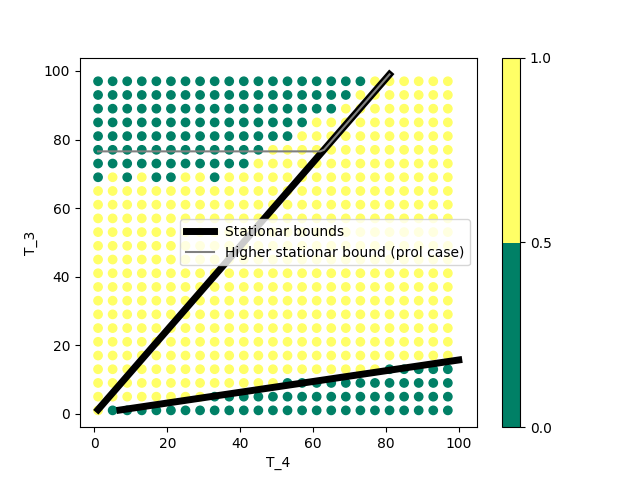
\includegraphics[scale=0.85]{0_1_thres_10_target_fact_.png} 
\caption{Области стационарности системы. $\lambda_3=0.1$, $L=10$}
\label{Experiment:stationar}
\end{figure}
На рис.~\ref{Experiment:stationar} представлены результаты экспериментов. По осям координат отложены значения $T_3$ длительности обслуживания требований потока $\Pi_3$ и значения $T_4$ длительности обслуживания требований потока $\Pi_2$. Желтым цветом обозначены точки, в которых было определено достижение системой стационарного режима. Темно-зеленым цветом обозначены случаи отсутствия стационарности. Кроме того на графике черным цветом изображена область стационарности, полученная из достаточных условий теоремы~\ref{sufficient:double:theorem}. 

Из графика видно, что желтая область выходит далеко за границы черных линий. Это свидетельствует о том, что достаточное условие, полученное в работе аналитически, не является необходимым. Ввод дополнительного режима продления по высоко приоритетному потоку при отсутвии большого числа требований по низкоприоритетному потоку позволяет существенно расширить область стационарности системы. Интуитивно данный результат ожидаем: при отсутствии требований по одному из потоков, другой поток получает дополнительный временной <<запас>> для обслуживания за счет продления.

Также на графике изображена область, ограниченная серой линией. Эта область получена эмпирическими рассуждениями и дает <<примерную>> оценку области стационарности для системы с продлением. Рассуждения для вывода этой границы основаны на подсчете <<среднего>> количества времени, освобождающегося для обслуживания требований потока $\Pi_2$ за счет продления.

\begin{figure}[h]
\centering
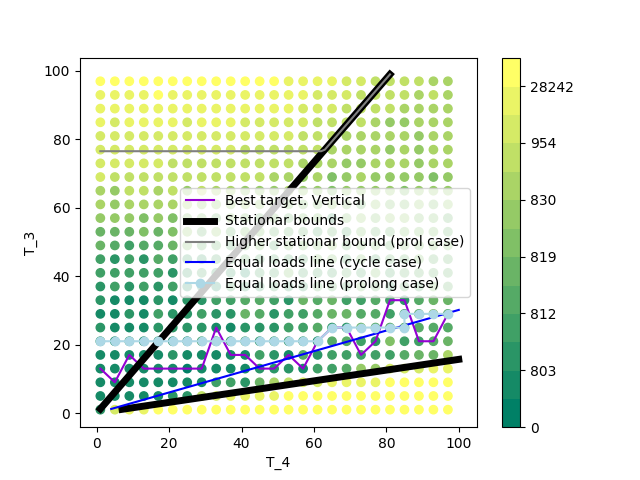
\includegraphics[scale=0.9]{0_1_thres_10_target.png} 
\caption{Поиск }
\label{Experiment:targets}
\end{figure}


Более детально результаты эксперимента представлены на рис.~\ref{Experiment:targets}. На этом рисунке каждому эксперименту соответствует посчитанная оценка средневзвешенной длительности ожидания одного требования. Чем более темным является цвет точки~--- тем лучше. Кроме присутствовавших на предыдущем рисунке границ, здесь присутствуют линии равных загрузок для случая циклического управления (синий цвет) и для случая циклического управления с продлением (голубой цвет). В работах \cite{Fedotkin:A:2009} и \cite{Fedotkin:Rachinskaya:2016} было отмечено, что оптимальные значение параметров с точки зрения средневзвешенного времени пребывания находится вблизи ломаной равных квазизагрузок. При условии отсутствия продления ($T^{(2,3)}=0$),  под загрузкой системы, например, по потоку $\Pi_1$ естественно понимать величину
\begin{equation}
\frac{(T^{(2,1)} + T^{(2,2)})\lambda_1 \sum_{\nu\geqslant 1}\nu p_{\nu}^{(1)}}{[\mu_2 T^{(2,2)}]}.
\end{equation}
Тогда ломаную равных квазизагрузок определим из условия равенства загрузки системы по потокам $\Pi_1$ и $\Pi_3$:
\begin{equation}
\frac{(T^{(2,1)} + T^{(2,2)})\lambda_1 \sum_{\nu\geqslant 1}\nu p_{\nu}^{(1)}}{[\mu_2 T^{(2,2)}]}=
    \frac{(T^{(2,1)} + T^{(2,2)})\lambda_3 \sum_{\nu\geqslant 1}\nu p_{\nu}^{(3)}}{[\mu_3 T^{(2,1)}]}
\end{equation}
График этой кривой изображен на рисунке~\ref{Experiment:targets} синим цветом. 

Далее встает вопрос о том, что считать загрузкой системы в случае присутствия продления по низкоприоритетному потоку $\Pi_3$. В данной работе под загрузкой будем понимать отношение общего числа пришедших требований по потоку ($\Pi_1$ или $\Pi_3$) к общему числу обслуженных требований по этому потоку. Аналитически посчитать эти величины сложно, поэтому на графике представлена кривая равных загрузок, посчитанная на основе экспериментальных данных. Как видно из рисунка, такая кривая лучше <<следует>> за оптимальными значениями параметров, нежели кривая равных квазизагрузок для циклического алгоритма.

Поясним, что значит кривая равных квазизагрузоу лучше <<следует>> за оптимальными значениями параметров. Поставим задачу при фикисированном значении времени обслуживания потока $\Pi_2$ (величина $T_4$ на рис.~\ref{Experiment:targets}), найти такое значение времени обслуживания потока $\Pi_3$ (величина $T_3$ на рис.~\ref{Experiment:targets}), при котором достигается минимум средневзвешенного времени пребывания требования в системе. Фиолетовая линия на рис.~\ref{Experiment:targets} демонстрирует динамику этих значений при изменении времен $T_4$. Видно, что <<в среднем>> голубая линии лучше аппроксимирует фиолетовую кривую, чем синяя. Особенно в окрестности прямой $T_4=0$. 

Завершая анализ экспериментальных данных, отметим следующее.
\begin{itemize}
    \item При увеличении интенсивности потока $\Pi_2$ (или, что то же самое, интенсивности потока $\Pi_1$), область стационарности сужается (см.~Рис.~\ref{Experiment:intensities}).
    \item С увеличением порога $L$ продления, область стационарности увеличивается (см.~Рис.~). 
\end{itemize}
\begin{figure*}
\begin{multicols}{2}
    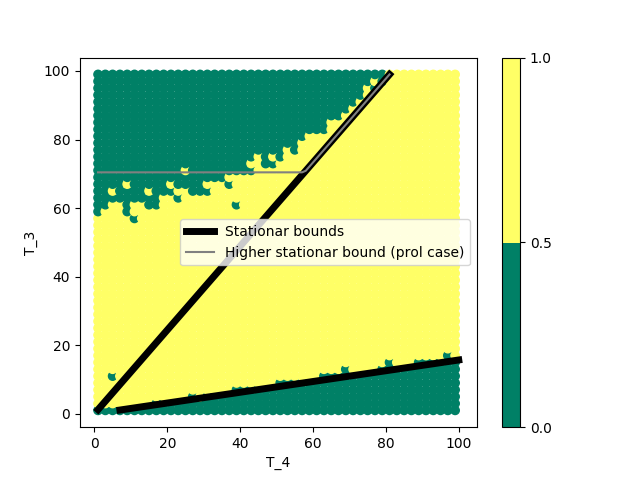
\includegraphics[width=1.2\linewidth]{0_1_thres_10_fact.png}\par 
    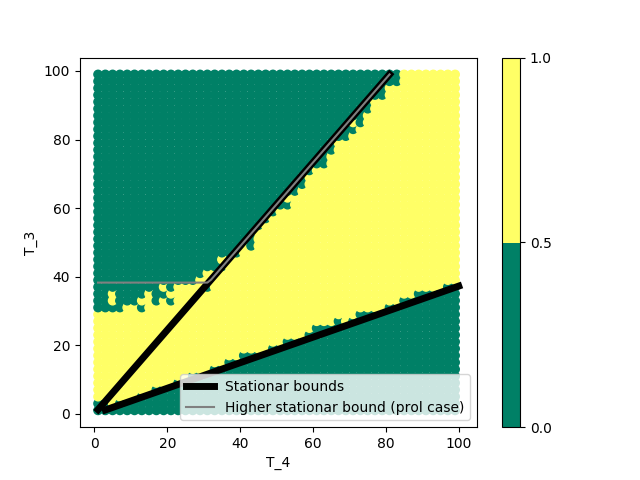
\includegraphics[width=1.2\linewidth]{0_2_thres_10_fact.png}\par 
    \end{multicols}
\caption{Области стационарности для разных значений $\lambda_1$. Слева $\lambda_1=0.1$, справа $\lambda_1=0.2$}
\label{Experiment:intensities}
\end{figure*}
\begin{figure*}
\begin{multicols}{2}
    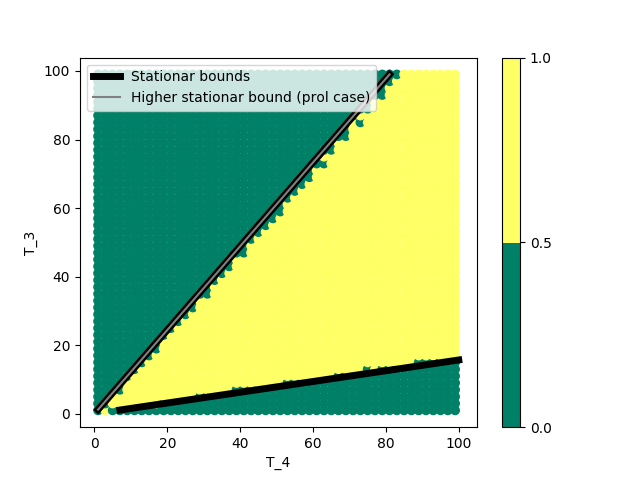
\includegraphics[width=1.15\linewidth]{0_1_thres_-1_fact.png}\par 
    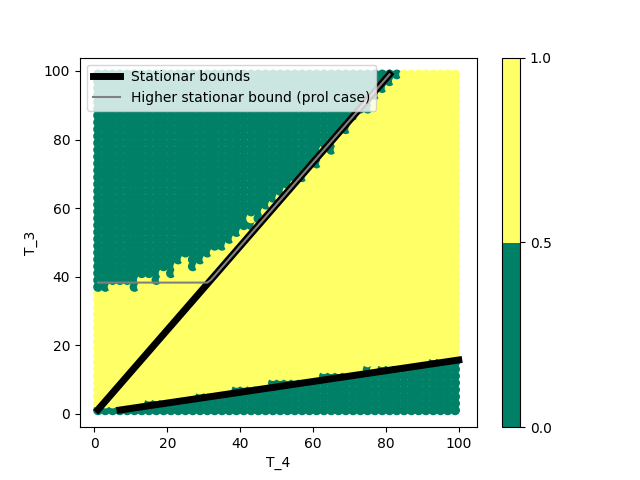
\includegraphics[width=1.15\linewidth]{0_1_thres_5_fact.png}\par 
    \end{multicols}
\begin{multicols}{2}
    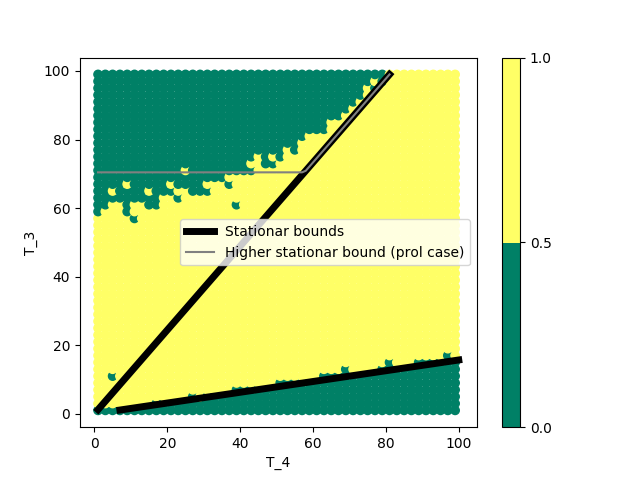
\includegraphics[width=1.15\linewidth]{0_1_thres_10_fact.png}\par
    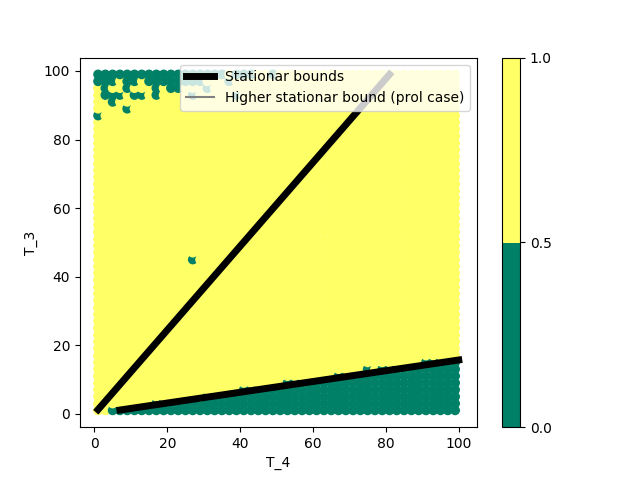
\includegraphics[width=1.15\linewidth]{0_1_thres_15_fact.png}\par
\end{multicols}
\caption{Области стационарности для разных значений $L$. Слева-направо, сверху-вниз $L=-1$; $5$; $10$; $15$}
\end{figure*}
\newpage
\section{Заключение}
В приведенной работе был рассмотрен тандем управляющих систем, управление в которых осуществляется по циклическому алгоритму и алгоритму с продлением. Основные результаты работы заключаются в следующем.

    \begin{enumerate}
        \item Построена строгая математическая модель тандема с циклическим алгоритмом управления и алгоритмом с продлением. Отличительностью особенностью системы также является немгновенность перемещения требований между системами. 
        \item Доказана марковость случайной последовательности, включающей длину низкоприоритетной очереди. Проведена классификация состояний цепи по арифметическим свойствам переходных вероятностей этой последовательности. А также найдены достаточное и необходимое условия существования стационарного распределения.
        \item Проведен аналогичный анализ для случайной последовательности, включающей очереди первичных требований: доказана ее марковость, проведена классификация состояний и найдено достаточное условие существования стационарного распределения.
        \item Найдено условие ограниченности для последовательности математических ожиданий $    \{( E\varkappa_{4,i}); i \geqslant 0\}/. 
$.
        \item Разработана имитационная модель для изучения исходной системы и написана программа ее реализующая.
        \item На основе имитационной модели были подтверждены и расширены результаты, полученные теоретически.
    \end{enumerate}







\newpage
\begin{thebibliography}{99}
% Не удаляйте следующую строчку!
\addcontentsline{toc}{section}{Литература}
\bibitem{Afanasyeva:Bulinskaya:2010} Афанасьева~Л.Г., Булинская~Е.В. Математические модели транспортных систем, основанные на теории очередей // Труды Московского физико-технического института (государственного университета).~--- 2010.~-- Т.~2~--- \No{}~4.~--- С.~6--21.
\bibitem{Borovkov:1980} Боровков~А.А. Асимптотические методы в теории массового обслуживания.~--- Наука, 1980.~--- 384~с.
\bibitem{Borovkov:1972} Боровков~А.А. Вероятностные процессы в теории массового обслуживания.~--- Рипол Классик, 1972.~--- 368~с.
\bibitem{Bocharov:1995} Бочаров~П.П., Печинкин~А.В. Теория массового обслуживания.~--- М.: Издательство РУДН, 1995.~--- 529~с.
\bibitem{Klimenok:Dudin:2004} Бройер~Л., Дудин~А.Н., Клименок~В.И., Царенков~Г.В. Двухфазная система $BMAP|G|1|N \to PH|1|M-1-1$ с блокировкой // Автомат. и телемех.~--- 2004.~--- \No{}~1.~--- Pp.~117–-130.

\bibitem{Gnedenko} Гнеденко~Б.В. Курс теории вероятностей.~--- М.:~Издательство ЛКИ, 2007.~--- 448~с.
\bibitem{Gnedenko:2012} Гнеденко~Б.В., Коваленко~И.Н. Введение в теорию массового обслуживания.~--- ЛКИ, 2012.~--- 400~с.
\bibitem{Zorine:2011:1} Зорин~А.В. Кибернетический подход к построению и анализу математической модели тандема двух перекрестков // Проблемы теоретической кибернетики. Материалы XVI Международной конференции (Нижний Новгород, 20-25 июня 2011 г.). Под ред. Ю.И. Журавлева. Нижний Новгород: Изд-во Нижегородского университета.~--- 2011.~--- С.~179--183.
\bibitem{Zorine:2011:2} Зорин~А.В. Устойчивость тандема систем обслуживания с бернуллиевским немгновенным перемещением требований // Теория вероятностей и математическая статистика.~--- 2011.~--- Вып.~84.~--- С.~163-176.
\bibitem{Kemeny} Кемени~Дж., Снелл~Дж., Кнепп~А. Счетные цепи Маркова.~--- М.:~Наука, 1987.~-- 416~с.
\bibitem{Klimenok:2015} Клименок~В.И., Савко~Р.Ч. Двухфазная система с повторными попытками и нетерпеливостью запросов // Автомат. и телемех., 2015.~--- \No{}~8.~--- Pp.~78–-93. 
\bibitem{Klimenok:2010} Клименок~В.И., Тарамин~О.С. Двухфазная система обслуживания с групповым марковским потоком и повторными вызовами // Автомат. и телемех.~--- 2010.~--- \No~1.~-- Pp.~3–-17 
\bibitem{Klimenok:2011} Клименок~В.И., Тарамин~О.С. Двухфазная система $GI/PH/1 \to /PH/1/0GI/PH/1 \to /PH/1/0$ с потерями // Автомат. и телемех.~--- 2011.~--- \No{}~5.~--- P.~113–-126.
\bibitem{Klimov:1966} Климов~Г.П. Стохастические системы обслуживания.~--- М.:~Наука, 1966.~--- 243~с.
\bibitem{Kolmogorov:1974} Колмогоров~А.Н. Основные понятия теории вероятностей.~--- М.:~Наука, 1974.~--- 120~с.
\bibitem{Kolmogorov:2006} Колмогоров~А.Н., Фомин~С.В. Элементы теории функций и функционального анализа.~--- М.:~Физматилит, 2006.~--- 572~с.
\bibitem{Kocheganov:2017:3} Кочеганов~В.М., Зорин~А.В. Анализ потоков первичных требований в тандеме при циклическом управлении с продлением // Информационные технологии и математическое моделирование (ИТММ--2017): Материалы XVI Международной конференции имени А.Ф. Терпугова (29 сентября -- 3 октября 2017 г.) -- Томск: Изд-во~НТЛ.~--- 2017.~--- Ч.~1.~--- С.81--87.
\bibitem{Kocheganov:2015:1} Кочеганов~В.М., Зорин~А.В. Вероятностная модель тандема систем массового обслуживания с циклическим управлением с продлением // Теория вероятностей, случайные процессы, математическая статистика и приложения: материалы Междунар. науч. конф., посвящ. 80-летию проф., д-ра физ.-мат. наук Г.А. Медведева, Минск, 23–26 февр.~--- 2015.~--- С.~94-–99.
\bibitem{Kocheganov:2015:2} Кочеганов~В.М., Зорин~А.В. Дискретная модель колебания длины низкоприоритетной очереди в тандеме систем массового обслуживания при циклическом алгоритме с продлением // Дискретные модели в теории управляющих систем: IX Международная конференция, Москва и Подмосковье, 20–22 мая.~--- 2015.~--- С.~126--129.
\bibitem{Kocheganov:2017:1} Кочеганов~В.М., Зорин~А.В. Достаточное условие существования стационарного режима низкоприоритетной очереди в тандеме систем массового обслуживания // Вестник Волжской государственной академии водного транспорта.~--- 2017.~--- Выпуск~50.~--- С.~47--55.
\bibitem{Kocheganov:2018:1} Кочеганов~В.М., Зорин~А.В. Достаточное условие существования стационарного режима очередей первичных требований в тандеме систем массового обслуживания // Вестник ТвГУ. Серия: Прикладная математика.~--- 2018.~--- №~2.~--- С.~49--74.
\bibitem{Kocheganov:2017:2} Кочеганов~В.М., Зорин~А.В. Изучение процесса управления потоками первичных требований в тандеме систем обслуживания с циклическим алгоритмом с продлением // Проблемы теоретической кибернетики: XVIII международная конференция (Пенза, 19--23 июня 2017~г.): Материалы : Под редакцией Ю.И.~Журавлева.~--- М.:~МАКС~Пресс.~--- 2017.~--- С.~135--137.

\bibitem{Neymark:Fedotkin:1968} Неймарк~Ю.И., Преображенская~А.М., Федоткин~М.А. Работа автомата с обратной связью, управляющего уличным движением на перекрестке // Изв. АН СССР, Техническая кибернетика.~--- 1968.~--- \No{}~5.~--- С.~129—-141. 
\bibitem{Neymark:Fedotkin:1967} Неймарк~Ю.И., Федоткин~М.А. О работе автомата, регулирующего уличное движение на перекрестке // Автоматика и телемеханика.~--- 1967.~--- \No{}~3.~--- С.~78-—87.  

\bibitem{Rachinskaya:Fedotkin:2012} Рачинская~М.А., Федоткин~М.А. Изучение характеристик потока машин в условиях малой плотности // Нижегородский государственный университет им.~Н.И.~Лобачевского, Нижний Новгород, 2012.~--- 36~с.~--- Деп. в ВИНИТИ 26.01.12, \No{}~27--В2012.
\bibitem{Saati:1971} Саати~Т. Элементы теории массового обслуживания и ее применение.~--- М.: Советское радио, 1971.~--- 520~с.
\bibitem{Fedotkin:A:2009} Федоткин~М.А. Анализ и оптимизация выходных процессов при циклическом управлении конфликтными транспортными потоками Гнеденко-Коваленко  // Автоматика и телемеханика, РАН.~--- 2009.~--- \No{}~12.~--- С.~92--108.
\bibitem{Fedotkin:2009} Федоткин~М.А. Математические модели на автомагистрали и на управляемом по циклическому алгоритму перекрестке // Нижегородский государственный университет им.~Н.И.~Лобачевского, Нижний Новгород.~--- 2009.~--- 30~с.~--- Деп. в ВИНИТИ, \No{}~5-V2009.
\bibitem{Fedotkin:1998} Федоткин~М.А. Нелокальный способ задания управляемых случайных процессов // Математические вопросы кибернетики.~--- М.: Наука.~--- 1998.~--- Вып.~7.~--- С.~333--344.
\bibitem{Fedotkin:1988} Федоткин~М.А. Оптимальное управление конфликтными потоками и маркированные точечные процессы с выделенной дискретной компонентой. 1 // Литовский математический сборник.~--- 1988.~--- Т.~28.~--- \No{}~4.~--- С.~783--784.
\bibitem{Fedotkin:1989} Федоткин~М.А. Оптимальное управление конфликтными потоками и маркированные точечные процессы с выделенной дискретной компонентой. 2 // Литовский математический сборник.~--- 1989.~--- Т.~29.~--- \No{}~1.~--- С.~148--159.
\bibitem{Fedotkin:1976} Федоткин М.А. О существовании эргодического распределения в системе с переменной структурой обслуживания конфликтных потоков // Теория вероятн. и ее примен.~--- 1976.~--- Т.~21~--- В.~4.~--- С.~792—-801.
\bibitem{Fedotkin:1996} Федоткин~М.А. Процессы обслуживания и управляющие системы // Математические вопросы кибернетики.~--- М.:~Наука.~--- 1996.~--- Вып.~6.~--- С. 51--70.
\bibitem{Fedotkin:2001} Федоткин~М.А. Управление процессами обслуживания // Вестник Нижегородского госуниверситета им.~Н.И.~Лобачевского “Математическое моделирование и оптимальное управление”.~--- 2001.~--- Вып.~2(24).~--- С.~169--188.
\bibitem{Fedotkin:Rachinskaya:2016} Федоткин~М.А., Рачинская~М.А. Имитационная модель циклического управления конфликтными неординарными пуассоновскими потоками // Вестник Волжской государственной академии водного транспорта.~---
2016.--- \No{}~47.~--- С.~43---51.
\bibitem{Rachinskaya:Fedotkin:2011:2} Федоткин~М.А., Рачинская~М.А. Исследование математической модели трафика автомобилей на основе подхода Ляпунова~--Яблонского // Материалы XVI Международной конференции «Проблемы теоретической кибернетики», Нижний Новгород: Изд-во Нижегородского госуниверситета.~--- 2011.~-- С.~508--512.
\bibitem{Hinchin:2010} Хинчин~А.Я. Работы по математической теории массового обслуживания.~--- Либроком, 2010.~--- 240~с.
\bibitem{Shiryaev} Ширяев~А.Н. Вероятность: в 2-х кн. Кн.~1.~--- М.:~Наука, 2007.~--- 552~с.
\bibitem{Yakushev:1990} Якушев~Ю.Ф. Об оптимальном обслуживании конфликтных потоков //  Теория вероятн. и ее примен, 1990.~--- Т.~35~--- В.~1~--- С.~161–-167.




\bibitem{Afanasyeva:Bulinskaya:2013:2} Afanasyeva~L.G., Bulinskaya~E.V. Asymptotic analysis of traffic lights performance under heavy traffic assumption // Methodology and Computing in Applied Probability, Springer.~--- 2013.~--- V.~15.~--- \No{}~4.~--- Pp.~935-–950.
\bibitem{Afanasyeva:Bulinskaya:2013:1} Afanasyeva~L.G., Bulinskaya~E.V. Estimation of transport systems capacity // Springer-Verlag Berlin, Heidelberg.~--- 2013.~--- Pp.~63–-77.
\bibitem{Asmussen:2008} Asmussen~S. Applied probability and queues.~--- Springer Science and Business Media, 2008.~--- V.~51.~--- 438~p.
\bibitem{Balsamo:2003} Balsamo~S., Persone~V.D.N., Inverardi~P. A review on queueing network models with finite capacity queues for software architectures performance prediction // Performance Evaluation 51.~--- 2003.~--- Pp.~269–-288.
\bibitem{Bartlet:1963} Bartlett, M.S., The Spectral Analysis of Point Processes // J. R. Statist. Soc. B.~--- 1963.~--- V.~25.~--- \No{}~2.~--- Pp.~264–-296.
\bibitem{Darroch:1964} Darroch~J.N. On the traffic-light queue // The Annals of Mathematical Statistics.~--- 1964.~--- V.~35~--- \No{}~1.~--- Pp.~380--388. 
\bibitem{Drew:1968} Drew~D.R. Traffic Stream Theory and Control.~--- New York: McGraw-Hill, 1968.
\bibitem{Erlang:1917} Erlang~A.K. Solution of some problems in the theory of probabilities of significance in automatic telephone exchanges // Elektrotkeknikeren.~--- 1917.~--- V.~13.~--- Pp.~5--13.
\bibitem{Erlang:1909} Erlang~A.K.  The Theory of Probabilities and Telephone Conversations //  Nyt Tidsskrift for Matematik.~--- 1909.~--- V.~20.~--- Pp.~33--39.
\bibitem{Fedotkin:Kudryavcev:Rachinskaya:2010} Fedotkin~M.A., Kudryavtsev~E.V., Rachinskaya~M.A.  About correctness of probabilistic models of traffic flows dynamics on a motorway // Proceedings 36 of International Workshop «Distributed computer and communication networks» (DCCN-2010), Moscow.~--- 2010.~--- Pp.86--93.
\bibitem{Fedotkin:Kudryavcev:Rachinskaya:2011} Fedotkin~M.A., Kudryavtcev~E.V., Rachinskaya~M.A. Simulation and Research of Probabilistic Regularities in Motion of Traffic Flows // Proceedings of the International Workshop «Applied Methods of Statistical Analysis. Simulations and
Statistical Inference» AMSA’2011, Novosibirsk: Publishing house of NSTU.~--- 2011.~--- Pp.~11--18.
\bibitem{Rachinskaya:Fedotkin:2011:1} Fedotkin~M.A., Rachinskaya~M.A. Investigation of Traffic Flows Characteristics in Case of the Small Density // Queues: Flows, Systems, Networks. Proceedings of the International Conference «Modern Probabilistic Methods for Analysis and Optimization of Information and Telecommunication Networks». Minsk: BSU-RIVH.~--- 2011.~--- \No{}~21.~--- Pp.~82--87.
\bibitem{Rachinskaya:Fedotkin:2013} Fedotkin~M.A., Rachinskaya~M.A. Parameters estimator of the probabilistic model of batches traffic flow with the non-intensive movement // Proceedings of International Workshop «Distributed computer and communication networks» (DCCN-2013), Moscow.~--- 2013~--- Pp.~357--364.
\bibitem{Rachinskaya:Fedotkin:2014} Fedotkin~M., Rachinskaya~M. Parameters estimator of the probabilistic model of moving batches traffic flow // Distributed Computer and Communication Networks. Springer International Publishing, «Communications in Computer and Information Science» series.~--- 2014.~--- V.~279.~--- Pp.~154--168.

\bibitem{Ferguson:1985} Ferguson~М.J., Aminetzah~Y.J. Exact results for nonsymmetric token ring systems // IEEE Transactions on Communications.~--- 1985.~--- V.~33.~--- \No{}~3.~--- Pp.~223—-231.
\bibitem{Gnedenko:Konig:1983} Gnedenko~B.W., Konig~D. Handbuch der Bedienungstheorie // Akademie Verlag, Berlin, 1983.
\bibitem{Gomez:2002:3} Gomez-Corral~A. A matrix-geometric approximation for tandem queues with blocking and repeated attempts // Operations Research Letters  30.~--- 2002.~--- Pp.~360-–374.
\bibitem{Gomez:2002:1} Gomez-Corral~A. A tandem queue with blocking and Markovian arrival process // Queueing Systems 41.~--- 2002.~--- Pp.~343–-370. 
\bibitem{Gomez:2002:2} Gomez-Corral~A. On a tandem G-network with blocking // Advances in Applied Probability 34 (3).~--- 2002.~--- Pp.~626-–661.
\bibitem{Haight:1963} Haight~F.A. Mathematical Theories of Traffic Flow.~-- New York: Academic, 1963. 
\bibitem{Inose:1975} Inose~H., Hamada~T. Road Traffic Control.~--- Tokyo: Univ. of Tokyo Press, 1975.
\bibitem{Klimenok:Dudin:2005} Klimenok~V.I., Breuer~L., Tsarenkov~G.V., Dudin~A.N. The $BMAP/G/1/N \to PH/1/M$ system with losses // Performance Evaluation 61.~--- 2005.~--- Pp.~17-–40.



\bibitem{Kocheganov:2015:3} Kocheganov~V.M., Zorine~A.V. Low-priority queue Fluctuations in Tandem of Queuing Systems Under Cyclic Control with Prolongations // DCCN. Ser. Communications in Computer and Information Science. 2016.~--- V.~601.~--- Pp.~268--279.

 \bibitem{Kocheganov:2016} Kocheganov~V.M., Zorine~A.V. Low-priority queue and server's steady-state existence in a tandem under prolongable cyclic service // Distributed Computer and Communication Networks. DCCN~2016. Ser. Communications in Computer and Information Science.~--- 2016.~--- V.~678.~--- Pp.~210--221.
 
 \bibitem{Kocheganov:2017} Kocheganov~V., Zorine~A. Primary input flows in a tandem under prolongable cyclic service // Distributed Computer and Communication Networks. DCCN-2017.~--- 2017.~--- Pp.~517--525.

 
\bibitem{Perros:1994} Perros~H.G.  Queueing networks with blocking, in: Exact and Approximate Solutions // Oxford University Press, New York.~--- 1994.
\bibitem{Perros:1989} Perros~H.G. A bibliography of papers on queueing networks with finite capacity queues // Performance Evaluation 10.~--- 1989.~-- P.~255–260.
\bibitem{Pollaczek:1934} Pollaczek~F. Uber das warteproblem // Mathematische Zeitschrift.~--- 1934.~--- V.~38.~--- \No{}.~1.~--- Pp.~492--537.

\bibitem{Reich:1957} Reich~E.  Waiting times when queues are in tandem // The Annals of Mathematical Statistics.~--- 1957.~--- V.28.~--- \No{}3.~--- P.~768--773.

\bibitem{Takagi:1985} Takagi~H. Mean message waiting times in symmetric multiqueue systems with cyclic service // Performance Evaluation.~--- 1985.~--- V.~5.~--- \No{}~4~--- Pp.~271—-277.  
\bibitem{Zorine:2010} Zorine~.A.V. Stability of a tandem queuing system with delayed Bernoulli transition of customers // Abstracts of international conference "Modern stochastics: theory and applications II" Dedicated to the anneversaries of prominent Ukranian scientists: Anatolij Skorokhod, Volodymyr Korolyuk and Igor Kovalenko, Kyiv, Ukrain, September 7-11.~--- 2010.~--- Pp.~76.

\bibitem{Zorine:2013:2} Zorine~A.V. On the conditions for the existence of a stationary mode in a tandem of queuing systems with cyclic control in a random environment // Automatic Control and Computer Sciences.~--- 2013.~--- V.~47.~--- Pp.~183--191.
\bibitem{Zorine:2012} Zorine~A.V. Stability of a tandem of queueing systems with Bernoulli noninstantaneous transfer of customers // Theor. Probability and Math. Statist.~--- 2012.~--- V.84.~--- Pp.~173--188.
\bibitem{Zorine:2013:1} Zorine~A.V. Study of queues’ sizes in tandem intersections under cyclic control in random environment // Modern Probabilistic Methods for Analysis of Telecommunication Networks. Communications in Computer and Information Science.~--- 2013.~--- V.~356.~--- Pp.~206--215.

\end{thebibliography}

\end{document}



























Первая часть суммы соответствует случаю $(w_1, w_3)=(0,0)$. Из теоремы \eqref{prob:rek:1} следует:
\begin{multline*}
    Q_{1,i+1}(\tilde{\gamma},0,0) \times v_1^{0} v_3^{0} = Q_{1,i+1}(\tilde{\gamma},0,0) =\sum_{x_1=0}^{\ell(\tilde{k},\tilde{r},1)} \sum_{x_3=0}^{\ell(\tilde{k},\tilde{r},3)} \sum_{\gamma \in {\mathbb H}_{-1}(\tilde{\gamma},x_3)}Q_{1,i}(\gamma,x_1, x_3)\times \\ \times
\sum_{a=0}^{\ell(\tilde{k},\tilde{r},3)-x_3}\varphi_3(a,T^{(\tilde{k},\tilde{r})}) \times \sum_{a=0}^{\ell(\tilde{k},\tilde{r},1)-x_1}\varphi_1(a,T^{(\tilde{k},\tilde{r})})
\end{multline*}

Вторая часть суммы получается при $w_1=0$ и $w_3>0$: 
\begin{multline*}
   \sum_{w_3=1}^{\infty}  Q_{1,i+1}(\tilde{\gamma},0,w_3) \times v_1^{0} v_3^{w_3} = \sum_{w_3=1}^{\infty}  \sum_{x_1=0}^{\ell(\tilde{k},\tilde{r},1)} \sum_{x_3=0}^{w_3 + \ell(\tilde{k},\tilde{r},3)} \sum_{\gamma \in {\mathbb H}_{-1}(\tilde{\gamma},x_3)}Q_{1,i}(\gamma,x_1, x_3) \times  \\ \times \varphi_3(w_3 + \ell(\tilde{k},\tilde{r},3) - x_3,T^{(\tilde{k},\tilde{r})})  \times \sum_{a=0}^{\ell(\tilde{k},\tilde{r},1)-x_1}\varphi_1(a,T^{(\tilde{k},\tilde{r})}) \times v_1^{0} v_3^{w_3}
\end{multline*}
Поменяв порядок суммирования по $w_3$ и $x_3$, получим
\begin{multline*}
   \sum_{w_3=1}^{\infty}  Q_{1,i+1}(\tilde{\gamma},0,w_3) \times v_1^{0} v_3^{w_3} = \sum_{x_3=0}^{\ell(\tilde{k},\tilde{r},3)} \sum_{w_3=1}^{\infty}  \sum_{x_1=0}^{\ell(\tilde{k},\tilde{r},1)}  \sum_{\gamma \in {\mathbb H}_{-1}(\tilde{\gamma},x_3)}Q_{1,i}(\gamma,x_1, x_3) \times  \\
   \times \varphi_3(w_3 + \ell(\tilde{k},\tilde{r},3) - x_3,T^{(\tilde{k},\tilde{r})})  \times \sum_{a=0}^{\ell(\tilde{k},\tilde{r},1)-x_1}\varphi_1(a,T^{(\tilde{k},\tilde{r})})  \times  v_3^{w_3} + \\ 
   + \sum_{x_3=\ell(\tilde{k},\tilde{r},3)+1}^{\infty} \sum_{w_3=x_3 - \ell(\tilde{k},\tilde{r},3)}^{\infty}  \sum_{x_1=0}^{\ell(\tilde{k},\tilde{r},1)}  \sum_{\gamma \in {\mathbb H}_{-1}(\tilde{\gamma},x_3)}Q_{1,i}(\gamma,x_1, x_3) \times  \\ 
   \times \varphi_3(w_3 + \ell(\tilde{k},\tilde{r},3) - x_3,T^{(\tilde{k},\tilde{r})})  \times \sum_{a=0}^{\ell(\tilde{k},\tilde{r},1)-x_1}\varphi_1(a,T^{(\tilde{k},\tilde{r})}) \times  v_3^{w_3} 
\end{multline*}
Преобразуем получившиеся слагаемые. Сначала первое:
\begin{multline*}
\sum_{x_3=0}^{\ell(\tilde{k},\tilde{r},3)} \sum_{w_3=1}^{\infty}  \sum_{x_1=0}^{\ell(\tilde{k},\tilde{r},1)}  \sum_{\gamma \in {\mathbb H}_{-1}(\tilde{\gamma},x_3)}Q_{1,i}(\gamma,x_1, x_3) 
   \times \varphi_3(w_3 + \ell(\tilde{k},\tilde{r},3) - x_3,T^{(\tilde{k},\tilde{r})})  \times \\ 
   \times \sum_{a=0}^{\ell(\tilde{k},\tilde{r},1)-x_1}\varphi_1(a,T^{(\tilde{k},\tilde{r})}) \times v_3^{w_3} = 
\sum_{x_3=0}^{\ell(\tilde{k},\tilde{r},3)}\sum_{x_1=0}^{\ell(\tilde{k},\tilde{r},1)} \sum_{\gamma \in {\mathbb H}_{-1}(\tilde{\gamma},x_3)} Q_{1,i}(\gamma,x_1, x_3) \times \\
\times  \sum_{w_3=1}^{\infty}    
 \varphi_3(w_3 + \ell(\tilde{k},\tilde{r},3) - x_3,T^{(\tilde{k},\tilde{r})})  v_3^{w_3}  
 \times \sum_{a=0}^{\ell(\tilde{k},\tilde{r},1)-x_1}\varphi_1(a,T^{(\tilde{k},\tilde{r})}) = \\ =
 \sum_{x_3=0}^{\ell(\tilde{k},\tilde{r},3)}\sum_{x_1=0}^{\ell(\tilde{k},\tilde{r},1)} \sum_{\gamma \in {\mathbb H}_{-1}(\tilde{\gamma},x_3)} Q_{1,i}(\gamma,x_1, x_3) v_3^{x_3-\ell(\tilde{k},\tilde{r},3)} \times \\ \times \sum_{w_3=\ell(\tilde{k},\tilde{r},3) - x_3 + 1}^{\infty}    
 \varphi_3(w_3 ,T^{(\tilde{k},\tilde{r})})  v_3^{w_3}  \times \sum_{a=0}^{\ell(\tilde{k},\tilde{r},1)-x_1}\varphi_1(a,T^{(\tilde{k},\tilde{r})}) 
\end{multline*}
Теперь преобразуем второе:
\begin{multline*}
\sum_{x_3=\ell(\tilde{k},\tilde{r},3)+1}^{\infty} \sum_{w_3=x_3 - \ell(\tilde{k},\tilde{r},3)}^{\infty}  \sum_{x_1=0}^{\ell(\tilde{k},\tilde{r},1)}  \sum_{\gamma \in {\mathbb H}_{-1}(\tilde{\gamma},x_3)}Q_{1,i}(\gamma,x_1, x_3) 
   \times \varphi_3(w_3 + \ell(\tilde{k},\tilde{r},3) - x_3,T^{(\tilde{k},\tilde{r})})   \times \\ \times \sum_{a=0}^{\ell(\tilde{k},\tilde{r},1)-x_1}\varphi_1(a,T^{(\tilde{k},\tilde{r})}) \times  v_3^{w_3} =
   \sum_{x_3=\ell(\tilde{k},\tilde{r},3)+1}^{\infty}   \sum_{x_1=0}^{\ell(\tilde{k},\tilde{r},1)}  \sum_{\gamma \in {\mathbb H}_{-1}(\tilde{\gamma},x_3)}Q_{1,i}(\gamma,x_1, x_3) v_3^{x_3-\ell(\tilde{k},\tilde{r},3)}\times  \\ 
   \times \sum_{a=0}^{\ell(\tilde{k},\tilde{r},1)-x_1}\varphi_1(a,T^{(\tilde{k},\tilde{r})}) \times \sum_{w_3=0}^{\infty} \varphi_3(w_3,T^{(\tilde{k},\tilde{r})})  \times   v_3^{w_3} 
\end{multline*}
Добавляя и вычитая одну и ту же сумму, получим
\begin{multline*}
\sum_{x_3=\ell(\tilde{k},\tilde{r},3)+1}^{\infty} \sum_{w_3=x_3 - \ell(\tilde{k},\tilde{r},3)}^{\infty}  \sum_{x_1=0}^{\ell(\tilde{k},\tilde{r},1)}  \sum_{\gamma \in {\mathbb H}_{-1}(\tilde{\gamma},x_3)}Q_{1,i}(\gamma,x_1, x_3) 
   \times \varphi_3(w_3 + \ell(\tilde{k},\tilde{r},3) - x_3,T^{(\tilde{k},\tilde{r})})   \times \\ \times \sum_{a=0}^{\ell(\tilde{k},\tilde{r},1)-x_1}\varphi_1(a,T^{(\tilde{k},\tilde{r})}) \times  v_3^{w_3} =
   \sum_{x_3=0}^{\infty}   \sum_{x_1=0}^{\ell(\tilde{k},\tilde{r},1)}  \sum_{\gamma \in {\mathbb H}_{-1}(\tilde{\gamma},x_3)}Q_{1,i}(\gamma,x_1, x_3) v_3^{x_3-\ell(\tilde{k},\tilde{r},3)}\times  \\ 
   \times \sum_{a=0}^{\ell(\tilde{k},\tilde{r},1)-x_1}\varphi_1(a,T^{(\tilde{k},\tilde{r})}) \times \sum_{w_3=0}^{\infty} \varphi_3(w_3,T^{(\tilde{k},\tilde{r})})  \times   v_3^{w_3}  - 
    \sum_{x_3=0}^{\ell(\tilde{k},\tilde{r},3)}   \sum_{x_1=0}^{\ell(\tilde{k},\tilde{r},1)}  \sum_{\gamma \in {\mathbb H}_{-1}(\tilde{\gamma},x_3)}Q_{1,i}(\gamma,x_1, x_3) v_3^{x_3-\ell(\tilde{k},\tilde{r},3)}\times  \\ 
   \times \sum_{a=0}^{\ell(\tilde{k},\tilde{r},1)-x_1}\varphi_1(a,T^{(\tilde{k},\tilde{r})}) \times \sum_{w_3=0}^{\infty} \varphi_3(w_3,T^{(\tilde{k},\tilde{r})})  \times   v_3^{w_3} 
\end{multline*}

Третья часть суммы получается при $w_1>0$ и $w_3=0$.
\begin{multline*}
   \sum_{w_1=1}^{\infty}  Q_{1,i+1}(\tilde{\gamma},w_1,0) \times v_1^{w_1} v_3^0 = \sum_{w_1=1}^{\infty}  \sum_{x_1=0}^{w_1+\ell(\tilde{k},\tilde{r},1)} \sum_{x_3=0}^{\ell(\tilde{k},\tilde{r},3)} 
   \sum_{\gamma \in {\mathbb H}_{-1}(\tilde{\gamma},x_3)}Q_{1,i}(\gamma,x_1, x_3) \times  \\ \times \varphi_1(w_1 + \ell(\tilde{k},\tilde{r},1) - x_1,T^{(\tilde{k},\tilde{r})})  \times \sum_{a=0}^{\ell(\tilde{k},\tilde{r},3)-x_3}\varphi_3(a,T^{(\tilde{k},\tilde{r})}) \times v_1^{w_1}
\end{multline*}
Поменяв порядок суммирования по $w_1$ и $x_1$, получим
\begin{multline*}
   \sum_{w_1=1}^{\infty}  Q_{1,i+1}(\tilde{\gamma},w_1,0) \times v_1^{w_1} = \sum_{x_1=0}^{\ell(\tilde{k},\tilde{r},1)} \sum_{w_1=1}^{\infty}  \sum_{x_3=0}^{\ell(\tilde{k},\tilde{r},3)}  \sum_{\gamma \in {\mathbb H}_{-1}(\tilde{\gamma},x_3)}Q_{1,i}(\gamma,x_1, x_3) \times  \\
   \times \varphi_1(w_1 + \ell(\tilde{k},\tilde{r},1) - x_1,T^{(\tilde{k},\tilde{r})})  \times \sum_{a=0}^{\ell(\tilde{k},\tilde{r},3)-x_3}\varphi_3(a,T^{(\tilde{k},\tilde{r})})  \times  v_1^{w_1} + \\ 
   + \sum_{x_1=\ell(\tilde{k},\tilde{r},1)+1}^{\infty} \sum_{w_1=x_1 - \ell(\tilde{k},\tilde{r},1)}^{\infty}  \sum_{x_3=0}^{\ell(\tilde{k},\tilde{r},3)}  \sum_{\gamma \in {\mathbb H}_{-1}(\tilde{\gamma},x_3)}Q_{1,i}(\gamma,x_1, x_3) \times  \\ 
   \times \varphi_1(w_1 + \ell(\tilde{k},\tilde{r},1) - x_1,T^{(\tilde{k},\tilde{r})})  \times \sum_{a=0}^{\ell(\tilde{k},\tilde{r},3)-x_1}\varphi_3(a,T^{(\tilde{k},\tilde{r})}) \times  v_1^{w_1} 
\end{multline*}
Преобразуем получившиеся слагаемые. Сначала первое:
\begin{multline*}
\sum_{x_1=0}^{\ell(\tilde{k},\tilde{r},1)} \sum_{w_1=1}^{\infty}  \sum_{x_3=0}^{\ell(\tilde{k},\tilde{r},3)}  \sum_{\gamma \in {\mathbb H}_{-1}(\tilde{\gamma},x_3)}Q_{1,i}(\gamma,x_1, x_3) 
   \times \varphi_1(w_1 + \ell(\tilde{k},\tilde{r},1) - x_1,T^{(\tilde{k},\tilde{r})})  \times \\ 
   \times \sum_{a=0}^{\ell(\tilde{k},\tilde{r},3)-x_3}\varphi_3(a,T^{(\tilde{k},\tilde{r})}) \times v_1^{w_1} = 
\sum_{x_1=0}^{\ell(\tilde{k},\tilde{r},1)}\sum_{x_3=0}^{\ell(\tilde{k},\tilde{r},3)} \sum_{\gamma \in {\mathbb H}_{-1}(\tilde{\gamma},x_3)} Q_{1,i}(\gamma,x_1, x_3) \times \\
\times  \sum_{w_1=1}^{\infty}    
 \varphi_1(w_1 + \ell(\tilde{k},\tilde{r},1) - x_1,T^{(\tilde{k},\tilde{r})})  v_1^{w_1}  
 \times \sum_{a=0}^{\ell(\tilde{k},\tilde{r},3)-x_3}\varphi_3(a,T^{(\tilde{k},\tilde{r})}) = \\ =
 \sum_{x_1=0}^{\ell(\tilde{k},\tilde{r},1)}\sum_{x_3=0}^{\ell(\tilde{k},\tilde{r},3)} \sum_{\gamma \in {\mathbb H}_{-1}(\tilde{\gamma},x_3)} Q_{1,i}(\gamma,x_1, x_3) v_1^{x_1-\ell(\tilde{k},\tilde{r},1)} \times \\ \times \sum_{w_1=\ell(\tilde{k},\tilde{r},1) - x_1 + 1}^{\infty}    
 \varphi_1(w_1 ,T^{(\tilde{k},\tilde{r})})  v_1^{w_1}  \times \sum_{a=0}^{\ell(\tilde{k},\tilde{r},3)-x_3}\varphi_3(a,T^{(\tilde{k},\tilde{r})}) 
\end{multline*}
Теперь преобразуем второе:
\begin{multline*}
\sum_{x_1=\ell(\tilde{k},\tilde{r},1)+1}^{\infty} \sum_{w_1=x_1 - \ell(\tilde{k},\tilde{r},1)}^{\infty}  \sum_{x_3=0}^{\ell(\tilde{k},\tilde{r},3)}  \sum_{\gamma \in {\mathbb H}_{-1}(\tilde{\gamma},x_3)}Q_{1,i}(\gamma,x_1, x_3) 
   \times \varphi_1(w_1 + \ell(\tilde{k},\tilde{r},1) - x_1,T^{(\tilde{k},\tilde{r})})   \times \\ \times \sum_{a=0}^{\ell(\tilde{k},\tilde{r},3)-x_3}\varphi_3(a,T^{(\tilde{k},\tilde{r})}) \times  v_1^{w_1} =
   \sum_{x_1=\ell(\tilde{k},\tilde{r},1)+1}^{\infty}   \sum_{x_3=0}^{\ell(\tilde{k},\tilde{r},3)}  \sum_{\gamma \in {\mathbb H}_{-1}(\tilde{\gamma},x_3)}Q_{1,i}(\gamma,x_1, x_3) v_1^{x_1-\ell(\tilde{k},\tilde{r},1)}\times  \\ 
   \times \sum_{a=0}^{\ell(\tilde{k},\tilde{r},3)-x_3}\varphi_3(a,T^{(\tilde{k},\tilde{r})}) \times \sum_{w_1=0}^{\infty} \varphi_1(w_1,T^{(\tilde{k},\tilde{r})})  \times   v_1^{w_1} 
\end{multline*}
Добавляя и вычитая одну и ту же сумму, получим
\begin{multline*}
\sum_{x_1=\ell(\tilde{k},\tilde{r},1)+1}^{\infty} \sum_{w_1=x_1 - \ell(\tilde{k},\tilde{r},1)}^{\infty}  \sum_{x_3=0}^{\ell(\tilde{k},\tilde{r},3)}  \sum_{\gamma \in {\mathbb H}_{-1}(\tilde{\gamma},x_3)}Q_{1,i}(\gamma,x_1, x_3) 
   \times \varphi_1(w_1 + \ell(\tilde{k},\tilde{r},1) - x_1,T^{(\tilde{k},\tilde{r})})   \times \\ \times \sum_{a=0}^{\ell(\tilde{k},\tilde{r},3)-x_3}\varphi_3(a,T^{(\tilde{k},\tilde{r})}) \times  v_1^{w_1} =
   \sum_{x_1=0}^{\infty}   \sum_{x_3=0}^{\ell(\tilde{k},\tilde{r},3)}  \sum_{\gamma \in {\mathbb H}_{-1}(\tilde{\gamma},x_3)}Q_{1,i}(\gamma,x_1, x_3) v_1^{x_1-\ell(\tilde{k},\tilde{r},1)}\times  \\ 
   \times \sum_{a=0}^{\ell(\tilde{k},\tilde{r},3)-x_3}\varphi_3(a,T^{(\tilde{k},\tilde{r})}) \times \sum_{w_1=0}^{\infty} \varphi_1(w_1,T^{(\tilde{k},\tilde{r})})  \times   v_1^{w_1}  - 
    \sum_{x_1=0}^{\ell(\tilde{k},\tilde{r},1)}   \sum_{x_3=0}^{\ell(\tilde{k},\tilde{r},3)}  \sum_{\gamma \in {\mathbb H}_{-1}(\tilde{\gamma},x_3)}Q_{1,i}(\gamma,x_1, x_3) v_1^{x_1-\ell(\tilde{k},\tilde{r},1)}\times  \\ 
   \times \sum_{a=0}^{\ell(\tilde{k},\tilde{r},3)-x_3}\varphi_3(a,T^{(\tilde{k},\tilde{r})}) \times \sum_{w_1=0}^{\infty} \varphi_1(w_1,T^{(\tilde{k},\tilde{r})})  \times   v_1^{w_1} 
\end{multline*}
И последний, четвертый вид слагаемых получается при $w_1>0$ и $w_3>0$
































\section{Потоки $\Pi_1$, $\Pi_3$, $\Pi_4$}

Введем для $y_1$, $y_4$, $\tilde{y}_1$,  $\tilde{y}_4 \in \mathbb{Z}_+$ и $t \in \mathbb{R}$, $t\geqslant 0$, функцию
\begin{multline}
\widetilde{\varphi}_{1,4}(k,r,t,y_1,\tilde{y}_1,y_4,\tilde{y}_4) =\\= (1-\delta_{\tilde{y}_1,0} )
  \varphi_1(\ell(k,r,1) - y_1 + \tilde{y}_1,t)
\times  \psi(\ell(k,r,1) + y_4 - \tilde{y}_4,y_4, p_{k,r}) + \\+\delta_{\tilde{y}_1,0} 
\sum_{a_1=0}^{\ell(k,r,1) - y_1}  \varphi_1(a_1,t)  \times  \psi(\min{\{\ell(k,r,1), y_1+a_1\}} + y_4 - \tilde{y}_4,y_4, p_{k,r})  
\label{tildephi:1:4}
\end{multline}


\begin{lemma}
Пусть $\Gamma^{(k_{i+1},r_{i+1})}=h(\Gamma^{(k_i,r_i)},x_{3,i})$, $i=0$, $1$, $\ldots$. Тогда в условиях теоремы~\ref{myTheorem} для $i \geqslant 0$ верны равенства
\begin{multline}
\Pr (\{ \omega \colon \varkappa_{1,i+1} = x_{1,i+1}, \varkappa_{3,i+1} = x_{3,i+1}, \varkappa_{4,i+1} = x_{4,i+1}\} |\mathop{\cap}\limits_{t=0}^{i}\{\omega\colon \Gamma_t=\Gamma^{(k_t,r_t)}, \varkappa_t=x^t\})=\\
=\widetilde{\varphi}_3(k_{i+1},r_{i+1},T^{(k_{i+1},r_{i+1})},x_{3,i},x_{3,i+1}) \times \widetilde{\varphi}_{1,4}(k_{i+1},r_{i+1},T^{(k_{i+1},r_{i+1})},x_{1,i},x_{1,i+1}, x_{4,i},x_{4,i+1}).
\label{kappa:1:kappa:3:kappa:4:conditional}
\end{multline}
\end{lemma}
\begin{proof}
Доказательство проводится аналогично доказательству предыдущего следствия. А именно, записывая по формуле полной вероятности с учетом формул \eqref{ProbablititiesToProve} и \eqref{eta:xi:forgetProperty}, имеем:
\begin{multline*}
\Pr (\{ \omega \colon \varkappa_{1,i+1} = x_{2,i+1}, \varkappa_{3,i+1} = x_{3,i+1},  \varkappa_{4,i+1} = x_{4,i+1} |\mathop{\cap}\limits_{t=0}^{i}\{\omega\colon \Gamma_t=\Gamma^{(k_t,r_t)}, \varkappa_t=x^t\}) =\\
=\sum_{a,b\in \mathbb{Z}_+^4} \varphi(a,k_i,r_i,x^i)\zeta(b,k_i,r_i,x^i) \times\\
    \times \Pr (\{ \omega \colon  \varkappa_{1,i+1} = x_{1,i+1}, \varkappa_{3,i+1} = x_{3,i+1},  \varkappa_{4,i+1} = x_{4,i+1} \} |\{\omega\colon \eta_i=a, \xi_i=b, \Gamma_i=\Gamma^{(k_i,r_i)}, \varkappa_i=x^i\}).
\end{multline*}

Из условий \eqref{queuesFunc} и \eqref{FourthFunc} следует
\begin{multline*}
\Pr (\{ \omega \colon  \varkappa_{1,i+1} = x_{1,i+1}, \varkappa_{3,i+1} = x_{3,i+1},  \varkappa_{4,i+1} = x_{4,i+1} \} |\mathop{\cap}\limits_{t=0}^{i}\{\omega\colon \Gamma_t=\Gamma^{(k_t,r_t)}, \varkappa_t=x^t\})=\\
= \sum_{a,b\in \mathbb{Z}_+^4} \varphi(a,k_i,r_i,x^i)\zeta(b,k_i,r_i,x^i)  \delta_{x_{1,i+1},\max\{0,x_{1,i}+a_1-b_1\}}   \delta_{x_{3,i+1},\max\{0,x_{3,i}+a_3-b_3\}}
\delta_{x_{4,i+1},x_{4,i}+a_4-a_2}
\end{multline*}
и, раскрывая $\varphi(\cdot, \cdot, \cdot, \cdot)$ и $\zeta(\cdot, \cdot, \cdot, \cdot)$, получим
\begin{multline*}
\Pr (\{ \omega \colon \varkappa_{1,i+1} = x_{1,i+1}, \varkappa_{3,i+1} = x_{3,i+1},  \varkappa_{4,i+1} = x_{4,i+1}\} |\mathop{\cap}\limits_{t=0}^{i}\{\omega\colon \Gamma_t=\Gamma^{(k_t,r_t)}, \varkappa_t=x^t\})=\\= \sum_{a_3,b_3\in \mathbb{Z}_+} \varphi_3(a_3,h_T(\Gamma^{(k_i,r_i)},x_{3,i})) \delta_{b_3,\ell(k_{i+1},r_{i+1},3)} \delta_{x_{3,i+1},\max\{0,x_{3,i}+a_3-b_3\}} \times \displaybreak[0]  \\
\times
\sum_{a_1,b_1\in \mathbb{Z}_+}  \varphi_1(a_1,h_T(\Gamma^{(k_i,r_i)},x_{3,i}))  \delta_{x_{1,i+1},\max\{0,x_{1,i}+a_1-b_1\}} \delta_{b_1,\ell(k_{i+1},r_{i+1},1)} \times \\ 
\times \sum_{a_2,b_2\in \mathbb{Z}_+} \psi(a_2,x_{4,i}, p_{k_{i+1},r_{i+1}}) \delta_{b_2,\ell(k_{i+1},r_{i+1},2)}
\times \sum_{a_4\in \mathbb{Z}_+} \delta_{a_4,\min{\{\ell(k_{i+1},r_{i+1},1), x_{1,i}+a_1}\}} \delta_{x_{4,i+1},x_{4,i}+a_4-a_2}     
\times  \\ \times
\sum_{b_4\in \mathbb{Z}_+}\delta_{b_4,x_{4,i}} \,.
\end{multline*}
И после упрощения сумм в предыдущем выражении, получим
\begin{multline*}
\Pr (\{ \omega \colon \varkappa_{1,i+1} = x_{1,i+1}, \varkappa_{3,i+1} = x_{3,i+1},  \varkappa_{4,i+1} = x_{4,i+1}\} |\mathop{\cap}\limits_{t=0}^{i}\{\omega\colon \Gamma_t=\Gamma^{(k_t,r_t)}, \varkappa_t=x^t\})=\\= \tilde{\varphi}_3(k_{i+1},r_{i+1}, h_T (\Gamma^{(k_i,r_i)},x_{3,i}), x_{3,i},x_{3,i+1}) \times \displaybreak[0]  \\
\times
\sum_{a_1\in \mathbb{Z}_+}  \varphi_1(a_1,h_T(\Gamma^{(k_i,r_i)},x_{3,i}))  \delta_{x_{1,i+1},\max\{0,x_{1,i}+a_1-\ell(k_{i+1},r_{i+1},1)\}} \times \\ 
\times \sum_{a_2=0}^{x_{4,i}} \psi(a_2,x_{4,i}, p_{k_{i+1},r_{i+1}}) 
\times \delta_{a_2,\min{\{\ell(k_{i+1},r_{i+1},1), x_{1,i}+a_1\}} + x_{4,i} - x_{4,i+1}} =\\
=\tilde{\varphi}_3(k_{i+1},r_{i+1}, h_T (\Gamma^{(k_i,r_i)},x_{3,i}), x_{3,i},x_{3,i+1}) \times \displaybreak[0]  \\
\times
\sum_{a_1\in \mathbb{Z}_+}  \varphi_1(a_1,h_T(\Gamma^{(k_i,r_i)},x_{3,i}))  \delta_{x_{1,i+1},\max\{0,x_{1,i}+a_1-\ell(k_{i+1},r_{i+1},1)\}} \times \\ 
\times  \psi(\min{\{\ell(k_{i+1},r_{i+1},1), x_{1,i}+a_1\}} + x_{4,i} - x_{4,i+1},x_{4,i}, p_{k_{i+1},r_{i+1}}) = \\
=\tilde{\varphi}_3(k_{i+1},r_{i+1}, h_T (\Gamma^{(k_i,r_i)},x_{3,i}), x_{3,i},x_{3,i+1}) \times \displaybreak[0]  \\
\times ( \delta_{x_{1,i+1},0} 
\sum_{a_1=0}^{\ell(k_{i+1},r_{i+1},1) - x_{1,i}}  \varphi_1(a_1,h_T(\Gamma^{(k_i,r_i)},x_{3,i}))  \times \\ \times \psi(\min{\{\ell(k_{i+1},r_{i+1},1), x_{1,i}+a_1\}} + x_{4,i} - x_{4,i+1},x_{4,i}, p_{k_{i+1},r_{i+1}})  + \\ + (1-\delta_{x_{1,i+1},0} )
  \varphi_1(\ell(k_{i+1},r_{i+1},1) - x_{1,i}+ x_{1,i+1},h_T(\Gamma^{(k_i,r_i)},x_{3,i}))
\times \\ 
\times  \psi(\ell(k_{i+1},r_{i+1},1) + x_{4,i} - x_{4,i+1},x_{4,i}, p_{k_{i+1},r_{i+1}})).
\end{multline*}
Поскольку $a_1$ изменяется в пределах $0\leqslant a_1 \leqslant \ell(k_{i+1},r_{i+1},1) + x_{1,i}$, то рассматриваемая вероятность упрощается следующим образом:
\begin{multline*}
    \Pr (\{ \omega \colon \varkappa_{1,i+1} = x_{1,i+1}, \varkappa_{3,i+1} = x_{3,i+1},  \varkappa_{4,i+1} = x_{4,i+1}\} |\mathop{\cap}\limits_{t=0}^{i}\{\omega\colon \Gamma_t=\Gamma^{(k_t,r_t)}, \varkappa_t=x^t\})=\\=
  \tilde{\varphi}_3(k_{i+1},r_{i+1}, h_T (\Gamma^{(k_i,r_i)},x_{3,i}), x_{3,i},x_{3,i+1}) \times \displaybreak[0]  \\
\times ( \delta_{x_{1,i+1},0} 
\sum_{a_1=0}^{\ell(k_{i+1},r_{i+1},1) - x_{1,i}}  \varphi_1(a_1,h_T(\Gamma^{(k_i,r_i)},x_{3,i}))  \times \\ \times \psi( x_{1,i}+a_1 + x_{4,i} - x_{4,i+1},x_{4,i}, p_{k_{i+1},r_{i+1}})  + \\ + (1-\delta_{x_{1,i+1},0} )
  \varphi_1(\ell(k_{i+1},r_{i+1},1) - x_{1,i}+ x_{1,i+1},h_T(\Gamma^{(k_i,r_i)},x_{3,i}))
\times \\ 
\times  \psi(\ell(k_{i+1},r_{i+1},1) + x_{4,i} - x_{4,i+1},x_{4,i}, p_{k_{i+1},r_{i+1}})).  
\end{multline*}

Лемма доказана.
\end{proof}



Докажем марковость последовательности $\{(\Gamma_i, \varkappa_{1,i},\varkappa_{3,i}, \varkappa_{4,i}); i \geqslant 0\}$.
\begin{theorem}
Пусть $\Gamma_0=\Gamma^{(k,r)}\in \Gamma$ и $(\varkappa_{1,0}, \varkappa_{3,0}, \varkappa_{4,0})=(x_{1,0}, x_{3,0}, x_{4,0})\in \mathbb{Z}_+^3$ фиксированы. Тогда последовательность $\{(\Gamma_i, \varkappa_{1,i},\varkappa_{3,i}, \varkappa_{4,i}); i \geqslant 0\}$ является однородной счетной цепью Маркова.
\end{theorem}
\begin{proof}
Действительно, поскольку $\Gamma_{i+1}$ функционально выражается через $\Gamma_i$ и $\varkappa_{3,i}$ (см.~\eqref{gammaFunc}), то
\begin{multline*}
\Pr (\{ \Gamma_{i+1} =\Gamma^{(k_{i+1},r_{i+1})},\varkappa_{1,i+1} = x_{1,i+1},\varkappa_{3,i+1} = x_{3,i+1},\varkappa_{4,i+1} = x_{4,i+1}\} |\cap_{t=0}^{i}\{ \Gamma_t=\Gamma^{(k_t,r_t)}, \varkappa_t=x^t\})=\\
=\delta_{\Gamma^{(k_{i+1},r_{i+1})},h(\Gamma^{(k_i,r_i)},x_{3,i})}\times \\ \times \Pr (\{ \varkappa_{1,i+1} = x_{1,i+1},  \varkappa_{3,i+1} = x_{3,i+1},\varkappa_{4,i+1} = x_{4,i+1}\} |\cap_{t=0}^{i}\{ \Gamma_t=\Gamma^{(k_t,r_t)}, \varkappa_t=x^t\}),
\end{multline*}
для $\Gamma^{(k_i,r_i)}\in \Gamma$, $(x_{1,i}, x_{3,i}, x_{4,i})\in {\mathbb Z}_+^3$, $i\geqslant 0$. Учитывая лемму \eqref{kappa:1:kappa:3:kappa:4:conditional}, убеждаемся, что вероятность 
\begin{multline*}
\Pr (\{ \Gamma_{i+1} =\Gamma^{(k_{i+1},r_{i+1})},\varkappa_{1,i+1} = x_{1,i+1},\varkappa_{3,i+1} = x_{3,i+1},\varkappa_{4,i+1} = x_{4,i+1}\} |\cap_{t=0}^{i}\{\Gamma_t=\Gamma^{(k_t,r_t)}, \varkappa_t=x^t\}) = \\
=\delta_{\Gamma^{(k_{i+1},r_{i+1})},h(\Gamma^{(k_i,r_i)},x_{3,i})} \times \widetilde{\varphi}_3(k_{i+1},r_{i+1},T^{(k_{i+1},r_{i+1})},x_{3,i},x_{3,i+1}) \times \\ \times \widetilde{\varphi}_{1,4}(k_{i+1},r_{i+1},T^{(k_{i+1},r_{i+1})},x_{1,i},x_{1,i+1}, x_{4,i},x_{4,i+1})
\end{multline*}
зависит только от значений $(\Gamma_i,\varkappa_{1,i},\varkappa_{3,i},\varkappa_{4,i})$ и $(\Gamma_{i+1},\varkappa_{1,i+1}, \varkappa_{3,i+1},\varkappa_{4,i+1})$. Следовательно, 
\begin{multline*}
\Pr (\{ \Gamma_{i+1} =\Gamma^{(k_{i+1},r_{i+1})},\varkappa_{1,i+1} = x_{1,i+1},\varkappa_{3,i+1} = x_{3,i+1},\varkappa_{4,i+1} = x_{4,i+1}\} |\cap_{t=0}^{i}\{\Gamma_t=\Gamma^{(k_t,r_t)}, \varkappa_t=x^t\})=\\
=\Pr (\{  \Gamma_{i+1} =\Gamma^{(k_{i+1},r_{i+1})},\varkappa_{1,i+1} = x_{1,i+1},\varkappa_{3,i+1} = x_{3,i+1},\varkappa_{4,i+1} = x_{4,i+1}\} | \\ \{ \Gamma_i=\Gamma^{(k_i,r_i)},\varkappa_{1,i}=x_{1,i}, \varkappa_{3,i}=x_{3,i}, \varkappa_{4,i}=x_{4,i}\}) = \\
=\Pr (\{ \Gamma_{i+1} =\Gamma^{(k_{i+1},r_{i+1})}, \varkappa_{1,i+1} = x_{1,i+1},\varkappa_{3,i+1} = x_{3,i+1},\varkappa_{4,i+1} = x_{4,i+1}\} |\\ |\cap_{t=0}^{i}\{ \Gamma_t=\Gamma^{(k_t,r_t)}, \varkappa_{1,t}=x_{1,t}, \varkappa_{3,t}=x_{3,t},\varkappa_{4,t}=x_{4,t}\}),
\end{multline*}
что доказывает марковость последовательности $\{(\Gamma_i, \varkappa_{1,i},\varkappa_{3,i},\varkappa_{4,i}); i \geqslant 0\}$.
\end{proof}





Обозначим для $\gamma \in \Gamma$ и $(x_1,x_3,x_4) \in {\mathbb Z}_+^3$
\begin{equation}
Q_{4,i}(\gamma,x_1,x_3,x_4) = \Pr(\Gamma_{i}=\gamma, \varkappa_{1,i}=x_1, \varkappa_{3,i}=x_3, \varkappa_{4,i}=x_4).
\end{equation}

\begin{theorem}
Пусть $\tilde{\gamma} =\Gamma^{(\tilde{k},\tilde{r})}\in \Gamma$ и $(\tilde{x}_1, \tilde{x}_3, \tilde{x}_4) \in {\mathbb Z}_+^3$. Тогда для переходных вероятностей $\{Q_{4,i}(\cdot,\cdot,\cdot,\cdot)\}_{i\geqslant 0}$ марковской цепи $\{(\Gamma_i, \varkappa_{1,i}, \varkappa_{3,i}, \varkappa_{4,i}); i \geqslant 0\} $ имеют место следующие рекуррентные соотношения:
\begin{multline*}
Q_{4,i+1}(\tilde{\gamma},0, 0, \tilde{x}_4)= 
\sum_{x_1=0}^{\ell(\tilde{k},\tilde{r},1)} \sum_{x_3=0}^{\ell(\tilde{k},\tilde{r},3)} \sum_{x_4=0}^{\infty}  \sum_{\gamma \in {\mathbb H}_{-1}(\tilde{\gamma},x_3)}Q_{4,i}(\gamma,x_1, x_3, x_4)\times \\ \times
\sum_{a=0}^{\ell(\tilde{k},\tilde{r},3)-x_3}\varphi_3(a,T^{(\tilde{k},\tilde{r})}) \times \sum_{a=0}^{\ell(\tilde{k},\tilde{r},1)-x_1}\varphi_1(a,T^{(\tilde{k},\tilde{r})}) \times
\psi( x_1+a + x_4 - \tilde{x}_4,x_4, p_{\tilde{k},\tilde{r}}),
\end{multline*}
\begin{multline*}
Q_{4,i+1}(\tilde{\gamma},0, \tilde{x}_3, \tilde{x}_4)= 
\sum_{x_1=0}^{\ell(\tilde{k},\tilde{r},1)} \sum_{x_3=0}^{\tilde{x}_3 + \ell(\tilde{k},\tilde{r},3)} \sum_{x_4=0}^{\infty} \sum_{\gamma \in {\mathbb H}_{-1}(\tilde{\gamma},x_3)}Q_{4,i}(\gamma,x_1, x_3, x_4) \times  \\ \times \varphi_3(\tilde{x}_3 + \ell(\tilde{k},\tilde{r},3) - x_3,T^{(\tilde{k},\tilde{r})})  \times   \sum_{a=0}^{\ell(\tilde{k},\tilde{r},1)-x_1}\varphi_1(a,T^{(\tilde{k},\tilde{r})})\times \\ \times \psi( x_1+a+ x_4 - \tilde{x}_4,x_4,p_{\tilde{k},\tilde{r}}), \quad \tilde{x}_3 > 0,
\end{multline*}
\begin{multline*}
Q_{4,i+1}(\tilde{\gamma},\tilde{x}_1, 0, \tilde{x}_4)= 
\sum_{x_1=0}^{\tilde{x}_1 + \ell(\tilde{k},\tilde{r},1) } \sum_{x_3=0}^{\ell(\tilde{k},\tilde{r},3)} \sum_{x_4=0}^{\infty} \sum_{\gamma \in {\mathbb H}_{-1}(\tilde{\gamma},x_3)}Q_{4,i}(\gamma,x_1, x_3, x_4) \times  \\ \times \sum_{a=0}^{\ell(\tilde{k},\tilde{r},3)-x_3}\varphi_3(a,T^{(\tilde{k},\tilde{r})}) \times \varphi_1(\tilde{x}_1 + \ell(\tilde{k},\tilde{r},1) - x_1,T^{(\tilde{k},\tilde{r})}) \times\\ \times \psi(\ell(\tilde{k},\tilde{r},1) + x_4 - \tilde{x}_4,x_4, p_{\tilde{k},\tilde{r}}), \quad \tilde{x}_1 > 0,
\end{multline*}
\begin{multline*}
Q_{4,i+1}(\tilde{\gamma},\tilde{x}_1, \tilde{x}_3, \tilde{x}_4)= 
\sum_{x_1=0}^{\tilde{x}_1 +\ell(\tilde{k},\tilde{r},1)} \sum_{x_3=0}^{\tilde{x}_3 +\ell(\tilde{k},\tilde{r},3)}  \sum_{x_4=0}^{\infty} \sum_{\gamma \in {\mathbb H}_{-1}(\tilde{\gamma},x_3)}Q_{4,i}(\gamma,x_1, x_3, x_4) \times  \\ \times \varphi_3(\tilde{x}_3 + \ell(\tilde{k},\tilde{r},3) - x_3,T^{(\tilde{k},\tilde{r})})  \times \varphi_1(\tilde{x}_1 + \ell(\tilde{k},\tilde{r},1)-x_1,T^{(\tilde{k},\tilde{r})}) \\ \times \psi(\ell(\tilde{k},\tilde{r},1) + x_4 - \tilde{x}_4,x_4, p_{\tilde{k},\tilde{r}}) , \quad \tilde{x}_1 > 0, \tilde{x}_3 > 0.
\end{multline*}
\label{prob:rek:1}
\end{theorem}
\begin{proof}
По формуле полной вероятности имеем
\begin{multline*}
Q_{4,i+1}(\tilde{\gamma},\tilde{x}_1,\tilde{x}_3,\tilde{x}_4) = \Pr(\Gamma_{i+1}=\tilde{\gamma}, \varkappa_{1,i+1}=\tilde{x}_1, \varkappa_{3,i+1}=\tilde{x}_3, \varkappa_{4,i+1}=\tilde{x}_4) = \\
= \sum_{x_1=0}^{\infty}\sum_{x_3=0}^{\infty}\sum_{x_4=0}^{\infty}\sum_{\gamma \in \Gamma} \Pr(\Gamma_{i}=\gamma, \varkappa_{1,i}=x_1, \varkappa_{3,i}=x_3, \varkappa_{4,i}=x_4) \times \\ \times  \Pr(\Gamma_{i+1}=\tilde{\gamma}, \varkappa_{1,i+1}=\tilde{x}_1, \varkappa_{3,i+1}=\tilde{x}_3,  \varkappa_{4,i+1}=\tilde{x}_4 | \Gamma_{i}=\gamma,\varkappa_{1,i}=x_1, \varkappa_{3,i}=x_3, \varkappa_{4,i}=x_4) =  \\ 
=\sum_{x_1=0}^{\infty} \sum_{x_3=0}^{\infty}\sum_{x_4=0}^{\infty}\sum_{\gamma \in \Gamma} Q_{4,i}(\gamma, x_1, x_3,x_4) \times \delta_{\tilde{\gamma},h(\gamma,x_3)}\times \\ \times
\Pr(\varkappa_{1,i+1}=\tilde{x}_1 , \varkappa_{3,i+1}=\tilde{x}_3, \varkappa_{4,i+1}=\tilde{x}_4 | \Gamma_{i}=\gamma, \varkappa_{1,i}=x_1, \varkappa_{3,i}=x_3, \varkappa_{4,i}=x_4).
\end{multline*}
%\widetilde{\varphi}_3(k_{i+1},r_{i+1},T^{(k_{i+1},r_{i+1})},x_{3,i},x_{3,i+1}) \times \widetilde{\varphi}_{1,4}(k_{i+1},r_{i+1},T^{(k_{i+1},r_{i+1})},x_{1,i},x_{1,i+1}, x_{4,i},x_{4,i+1})
Тогда из определения $ {\mathbb H}_{-1}(\tilde{\gamma},x_3)$ следует, что 
\begin{multline*}
Q_{4,i+1}(\tilde{\gamma},\tilde{x}_1, \tilde{x}_3, \tilde{x}_4) =\sum_{x_1=0}^{\infty} \sum_{x_3=0}^{\infty}\sum_{x_4=0}^{\infty}\sum_{\gamma \in {\mathbb H}_{-1}(\tilde{\gamma},x_3)} Q_{4,i}(\gamma,x_1, x_3, x_4) \times \\ \times 
\Pr(\varkappa_{1,i+1}=\tilde{x}_1, \varkappa_{3,i+1}=\tilde{x}_3, \varkappa_{4,i+1}=\tilde{x}_4 | \Gamma_{i}=\gamma, \varkappa_{1,i}=x_1, \varkappa_{3,i}=x_3, \varkappa_{4,i}=x_4)
\end{multline*}
и учитывая лемму \eqref{kappa:1:kappa:3:kappa:4:conditional} продолжаем цепочку выкладок
\begin{multline*}
Q_{4,i+1}(\tilde{\gamma},\tilde{x}_1, \tilde{x}_3, \tilde{x}_4)=\sum_{x_1=0}^{\infty} \sum_{x_3=0}^{\infty}\sum_{x_4=0}^{\infty}\sum_{\gamma \in {\mathbb H}_{-1}(\tilde{\gamma},x_3)} Q_{4,i}(\gamma,x_1,x_3,x_4) \times 
\widetilde{\varphi}_3(\tilde{k},\tilde{r},T^{(\tilde{k},\tilde{r})},x_3,\tilde{x}_3) \times \\ \times \widetilde{\varphi}_{1,4}(\tilde{k},\tilde{r},T^{(\tilde{k},\tilde{r})},x_1,\tilde{x}_1, x_4,\tilde{x}_4)
= \sum_{x_1=0}^{\infty} \sum_{x_3=0}^{\infty} \sum_{x_4=0}^{\infty} \sum_{\gamma \in {\mathbb H}_{-1}(\tilde{\gamma},x_3)} Q_{4,i}(\gamma,x_1, x_3, x_4) \times \\ \times
[ (1-\delta_{\tilde{x}_3,0})\varphi_3(\tilde{x}_3 + \ell(\tilde{k},\tilde{r},3) - x_3,T^{(\tilde{k},\tilde{r})}) +\delta_{\tilde{x}_3,0} \sum_{a=0}^{\ell(\tilde{k},\tilde{r},3)-x_3}\varphi_3(a,T^{(\tilde{k},\tilde{r})})] \times \\ 
\times 
[  \delta_{\tilde{x}_1,0} 
\sum_{a_1=0}^{\ell(\tilde{k},\tilde{r},1) - x_1}  \varphi_1(a_1,h_T(\Gamma^{(k,r)},x_3))  \times \\ \times \psi(\min{\{\ell(\tilde{k},\tilde{r},1), x_1+a_1\}} + x_4 - \tilde{x}_4,x_4, p_{\tilde{k},\tilde{r}})  + \\ + (1-\delta_{\tilde{x}_1,0} )
  \varphi_1(\ell(\tilde{k},\tilde{r},1) - x_1+ \tilde{x}_1,h_T(\Gamma^{(k,r)},x_3))
\times  \\ 
\times  \psi(\ell(\tilde{k},\tilde{r},1) + x_4 - \tilde{x}_4,x_4, p_{\tilde{k},\tilde{r}})].
\end{multline*}

Поскольку  $\varphi_i(x,t)=0$ для $x<0$, $i=1,2$, получаем утверждение теоремы.
\end{proof}










\section{Потоки $\Pi_2$, $\Pi_3$, $\Pi_4$}



\begin{lemma}
Пусть $\Gamma^{(k_{i+1},r_{i+1})}=h(\Gamma^{(k_i,r_i)},x_{3,i})$, $i=0$, $1$, $\ldots$. Тогда в условиях теоремы~\ref{myTheorem} для $i \geqslant 0$ верны равенства
\begin{multline}
\Pr (\{ \omega \colon \varkappa_{1,i+1} = x_{1,i+1}, \varkappa_{3,i+1} = x_{3,i+1}\} |\mathop{\cap}\limits_{t=0}^{i}\{\omega\colon \Gamma_t=\Gamma^{(k_t,r_t)}, \varkappa_t=x^t\})=\\
=\widetilde{\varphi}_3(k_{i+1},r_{i+1},h_T(\Gamma^{(k_i,r_i)},x_{3,i}),x_{3,i},x_{3,i+1}) \times \widetilde{\varphi}_1(k_{i+1},r_{i+1},h_T(\Gamma^{(k_i,r_i)},x_{3,i}),x_{1,i},x_{1,i+1}).
\label{kappa:1:kappa:3:conditional}
\end{multline}
\end{lemma}
\begin{proof}
Доказательство проводится аналогично доказательству предыдущего следствия. А именно, записывая по формуле полной вероятности с учетом формул \eqref{ProbablititiesToProve} и \eqref{eta:xi:forgetProperty}, имеем:
\begin{multline*}
\Pr (\{ \omega \colon \varkappa_{2,i+1} = x_{2,i+1}, \varkappa_{3,i+1} = x_{3,i+1},  \varkappa_{4,i+1} = x_{4,i+1} |\mathop{\cap}\limits_{t=0}^{i}\{\omega\colon \Gamma_t=\Gamma^{(k_t,r_t)}, \varkappa_t=x^t\}) =\\
=\sum_{a,b\in \mathbb{Z}_+^4} \varphi(a,k_i,r_i,x^i)\zeta(b,k_i,r_i,x^i) \times\\
    \times \Pr (\{ \omega \colon  \varkappa_{2,i+1} = x_{2,i+1}, \varkappa_{3,i+1} = x_{3,i+1},  \varkappa_{4,i+1} = x_{4,i+1} \} |\{\omega\colon \eta_i=a, \xi_i=b, \Gamma_i=\Gamma^{(k_i,r_i)}, \varkappa_i=x^i\}).
\end{multline*}

Из условий \eqref{queuesFunc} и \eqref{FourthFunc} следует
\begin{multline*}
\Pr (\{ \omega \colon  \varkappa_{2,i+1} = x_{2,i+1}, \varkappa_{3,i+1} = x_{3,i+1},  \varkappa_{4,i+1} = x_{4,i+1} \} |\mathop{\cap}\limits_{t=0}^{i}\{\omega\colon \Gamma_t=\Gamma^{(k_t,r_t)}, \varkappa_t=x^t\})=\\
= \sum_{a,b\in \mathbb{Z}_+^4} \varphi(a,k_i,r_i,x^i)\zeta(b,k_i,r_i,x^i)  \delta_{x_{2,i+1},\max\{0,x_{2,i}+a_2-b_2\}}   \delta_{x_{3,i+1},\max\{0,x_{3,i}+a_3-b_3\}}
\delta_{x_{4,i+1},x_{4,i}+a_4-a_2}
\end{multline*}
и, раскрывая $\varphi(\cdot, \cdot, \cdot, \cdot)$ и $\zeta(\cdot, \cdot, \cdot, \cdot)$, получим
\begin{multline*}
\Pr (\{ \omega \colon \varkappa_{2,i+1} = x_{2,i+1}, \varkappa_{3,i+1} = x_{3,i+1},  \varkappa_{4,i+1} = x_{4,i+1}\} |\mathop{\cap}\limits_{t=0}^{i}\{\omega\colon \Gamma_t=\Gamma^{(k_t,r_t)}, \varkappa_t=x^t\})=\\= \sum_{a_3,b_3\in \mathbb{Z}_+} \varphi_3(a_3,h_T(\Gamma^{(k_i,r_i)},x_{3,i})) \delta_{b_3,\ell(k_{i+1},r_{i+1},3)} \delta_{x_{3,i+1},\max\{0,x_{3,i}+a_3-b_3\}} \times \displaybreak[0]  \\
\times
\sum_{a_1\in \mathbb{Z}_+}  \varphi_1(a_1,h_T(\Gamma^{(k_i,r_i)},x_{3,i})) 
\times \sum_{a_2,b_2\in \mathbb{Z}_+} \psi(a_2,x_{4,i}, p_{k_{i+1},r_{i+1}}) \delta_{b_2,\ell(k_{i+1},r_{i+1},2)}
\delta_{x_{2,i+1},\max\{0,x_{2,i}+a_2-b_2\}}
\times \\ \times \sum_{a_4\in \mathbb{Z}_+} \delta_{a_4,\min{\{\ell(k_{i+1},r_{i+1},1), x_{1,i}+a_1}\}} \delta_{x_{4,i+1},x_{4,i}+a_4-a_2}     \times  \\ 
\times  \sum_{b_1\in \mathbb{Z}_+}\delta_{b_1,\ell(k_{i+1},r_{i+1},1)}    \times
\sum_{b_4\in \mathbb{Z}_+}\delta_{b_4,x_{4,i}} \,.
\end{multline*}
И после упрощения сумм в предыдущем выражении, получим
\begin{multline*}
\Pr (\{ \omega \colon \varkappa_{2,i+1} = x_{2,i+1}, \varkappa_{3,i+1} = x_{3,i+1},  \varkappa_{4,i+1} = x_{4,i+1}\} |\mathop{\cap}\limits_{t=0}^{i}\{\omega\colon \Gamma_t=\Gamma^{(k_t,r_t)}, \varkappa_t=x^t\})=\\= \sum_{a_3,b_3\in \mathbb{Z}_+} \varphi_3(a_3,h_T(\Gamma^{(k_i,r_i)},x_{3,i})) \delta_{b_3,\ell(k_{i+1},r_{i+1},3)} \delta_{x_{3,i+1},\max\{0,x_{3,i}+a_3-b_3\}} \times \displaybreak[0]  \\
\times
\sum_{a_1\in \mathbb{Z}_+}  \varphi_1(a_1,h_T(\Gamma^{(k_i,r_i)},x_{3,i})) 
\times \sum_{b_2\in \mathbb{Z}_+} \psi(a_2^*,x_{4,i}, p_{k_{i+1},r_{i+1}}) \delta_{b_2,\ell(k_{i+1},r_{i+1},2)}
\delta_{x_{2,i+1},\max\{0,x_{2,i}+a_2^*-b_2\}} =  \\
= \sum_{a_3\in \mathbb{Z}_+} \varphi_3(a_3,h_T(\Gamma^{(k_i,r_i)},x_{3,i})) \delta_{x_{3,i+1},\max\{0,x_{3,i}+a_3-\ell(k_{i+1},r_{i+1},3)\}} \times \displaybreak[0]  \\
\times
\sum_{a_1\in \mathbb{Z}_+}  \varphi_1(a_1,h_T(\Gamma^{(k_i,r_i)},x_{3,i})) 
\times \psi(a_2^*,x_{4,i}, p_{k_{i+1},r_{i+1}})
\delta_{x_{2,i+1},\max\{0,x_{2,i}+a_2^*-\ell(k_{i+1},r_{i+1},2)\}}
= \\ =
\tilde{\varphi}_3(k_{i+1},r_{i+1}, h_T (\Gamma^{(k_i,r_i)},x_{3,i}), x_{3,i},x_{3,i+1}) \times \displaybreak[0]  \\
\times
\sum_{a_1\in \mathbb{Z}_+}  \varphi_1(a_1,h_T(\Gamma^{(k_i,r_i)},x_{3,i})) 
\times \psi(a_2^*,x_{4,i}, p_{k_{i+1},r_{i+1}})
\delta_{x_{2,i+1},\max\{0,x_{2,i}+a_2^*-\ell(k_{i+1},r_{i+1},2)\}}.
\end{multline*}
где $a_2^* = \min{\{\ell(k_{i+1},r_{i+1},1), x_{1,i}+a_1\}} -x_{4,i+1}+ x_{4,i}$.
Следствие доказано.
\end{proof}






Докажем марковость последовательности $\{(\Gamma_i, \varkappa_{2,i},\varkappa_{3,i},\varkappa_{4,i}); i \geqslant 0\}$.
\begin{theorem}
Пусть $\Gamma_0=\Gamma^{(k,r)}\in \Gamma$ и $(\varkappa_{2,i},\varkappa_{3,i},\varkappa_{4,i})=(x_{2,0}, x_{3,0}, x_{4,0})\in \mathbb{Z}_+^3$ фиксированы. Тогда последовательность $\{(\Gamma_i, \varkappa_{2,i},\varkappa_{3,i},\varkappa_{4,i}); i \geqslant 0\}$ является однородной счетной цепью Маркова.
\end{theorem}
\begin{proof}
Действительно, поскольку $\Gamma_{i+1}$ функционально выражается через $\Gamma_i$ и $\varkappa_{3,i}$ (см.~\eqref{gammaFunc}), то
\begin{multline*}
\Pr (\{ \Gamma_{i+1} =\Gamma^{(k_{i+1},r_{i+1})},\varkappa_{2,i+1} = x_{2,i+1},\varkappa_{3,i+1} = x_{3,i+1}, \varkappa_{4,i+1} = x_{4,i+1}\} | \\ | \cap_{t=0}^{i}\{ \Gamma_t=\Gamma^{(k_t,r_t)}, \varkappa_t=x^t\})
=\delta_{\Gamma^{(k_{i+1},r_{i+1})},h(\Gamma^{(k_i,r_i)},x_{3,i})}\times\\ \times \Pr (\{ \varkappa_{2,i+1} = x_{2,i+1},  \varkappa_{3,i+1} = x_{3,i+1},  \varkappa_{4,i+1} = x_{4,i+1}\} |\cap_{t=0}^{i}\{ \Gamma_t=\Gamma^{(k_t,r_t)}, \varkappa_t=x^t\}),
\end{multline*}
для $\Gamma^{(k_i,r_i)}\in \Gamma$, $(x_{2,i}, x_{3,i}, x_{4,i})\in {\mathbb Z}_+^3$, $i\geqslant 0$. Учитывая равенство \eqref{kappa:1:kappa:3:conditional}, убеждаемся, что вероятность 
\begin{multline*}
\Pr (\{ \Gamma_{i+1} =\Gamma^{(k_{i+1},r_{i+1})},\varkappa_{1,i+1} = x_{1,i+1},\varkappa_{3,i+1} = x_{3,i+1}\} |\cap_{t=0}^{i}\{\Gamma_t=\Gamma^{(k_t,r_t)}, \varkappa_t=x^t\}) = \\
=\delta_{\Gamma^{(k_{i+1},r_{i+1})},h(\Gamma^{(k_i,r_i)},x_{3,i})} \times \widetilde{\varphi}_3(k_{i+1},r_{i+1},h_T(\Gamma^{(k_i,r_i)},x_{3,i}),x_{3,i},x_{3,i+1})
\times \\ \times \widetilde{\varphi}_1(k_{i+1},r_{i+1},h_T(\Gamma^{(k_i,r_i)},x_{3,i}),x_{1,i},x_{1,i+1})
\end{multline*}
зависит только от значений $(\Gamma_i,\varkappa_{1,i},\varkappa_{3,i})$ и $(\Gamma_{i+1},\varkappa_{1,i+1}, \varkappa_{3,i+1})$. Следовательно, 
\begin{multline*}
\Pr (\{ \Gamma_{i+1} =\Gamma^{(k_{i+1},r_{i+1})},\varkappa_{1,i+1} = x_{1,i+1},\varkappa_{3,i+1} = x_{3,i+1}\} |\cap_{t=0}^{i}\{\Gamma_t=\Gamma^{(k_t,r_t)}, \varkappa_t=x^t\})=\\
=\Pr (\{  \Gamma_{i+1} =\Gamma^{(k_{i+1},r_{i+1})},\varkappa_{1,i+1} = x_{1,i+1},\varkappa_{3,i+1} = x_{3,i+1}\} | \\ \{ \Gamma_i=\Gamma^{(k_i,r_i)},\varkappa_{1,i}=x_{1,i}, \varkappa_{3,i}=x_{3,i}\}) = \\
=\Pr (\{ \Gamma_{i+1} =\Gamma^{(k_{i+1},r_{i+1})}, \varkappa_{1,i+1} = x_{1,i+1},\varkappa_{3,i+1} = x_{3,i+1}\} |\\ |\cap_{t=0}^{i}\{ \Gamma_t=\Gamma^{(k_t,r_t)}, \varkappa_{1,t}=x_{1,t}, \varkappa_{3,t}=x_{3,t}\}),
\end{multline*}
что доказывает марковость последовательности $\{(\Gamma_i, \varkappa_{1,i},\varkappa_{3,i}); i \geqslant 0\}$.
\end{proof}


